

\documentclass[11pt, a4paper, twoside, openright]{book}

\usepackage{a4wide}
\usepackage{amsmath,amssymb, amsthm} % AMS math
\usepackage{color}
\usepackage{enumerate}
\usepackage{fancyhdr}
\usepackage{fancyvrb}
\usepackage{floatflt}
\usepackage{multirow}
\usepackage{url}
\usepackage{rotating}
\usepackage{placeins}
 \usepackage{todonotes}
\usepackage{listings}
\usepackage{minitoc}
\usepackage{nextpage}
\usepackage{parskip}
\usepackage{setspace} 
\usepackage{xspace}
\usepackage{float}
\usepackage{subfig}
\usepackage{subfloat}

\usepackage{makeidx}

\pdfcompresslevel=9

\setcounter{tocdepth}{1}
\setcounter{minitocdepth}{1}
\setcounter{secnumdepth}{3}


\pagestyle{fancyplain}
\renewcommand{\chaptermark}[1]%
        {\markboth{\chaptername\ \thechapter\ \ #1}{}}
\renewcommand{\sectionmark}[1]%
        {\markright{\thesection\ \ #1}}
\fancyhead[LE,RO]{\fancyplain{}{\thepage}}
\fancyhead[RE]{\fancyplain{}{\it\leftmark}}
\fancyhead[LO]{\fancyplain{}{\it\rightmark}}
\fancyfoot[C]{\fancyplain{\thepage}{}}                                         

\setlength{\headheight}{15pt} 

\newcommand{\thesischapter}[1]{\chapter{#1}\minitoc}

\usepackage{stmaryrd, hyphenat}
\usepackage{graphicx}
\usepackage{wrapfig}
\usepackage{verbatim} 
\usepackage{mathtools}
\usepackage{xspace}
\usepackage{bussproofs}
\usepackage{multirow}
\usepackage{framed}
\usepackage{listings}
\usepackage{afterpage}
\lstset{numbers = left , stepnumber = 1 ,  framexleftmargin=30pt, frame = single}

\providecommand{\Monus}{% Don't redefine it if available
  \mathbin{% We want a binary operation
    \vphantom{+}% The same height as a plus or minus
    \text{% Change size in sub/superscripts
      \mathsurround=0pt % To be on the safe side
      \ooalign{% Superimpose the two symbols
        \noalign{\kern-.35ex}% but the dot is raised a bit
        \hidewidth$\smash{\cdot}$\hidewidth\cr % Dot
        \noalign{\kern.35ex}% Backup for vertical alignment
        $-$\cr % Minus
      }%
    }%
  }%
}

\newcommand{\mybar}{\mbox{\Large \textbar}}
\newcommand{\mypause}{\pause}
\newcommand{\var}[1]{\mathrm{Var}(#1)}
\newcommand{\freevar}[1]{\mathrm{FreeVar}(#1)}



% \newenvironment{proof}[1][Proof]{\begin{trivlist}
% \item[\hskip \labelsep {\bfseries #1}]}{\end{trivlist}}


\newcommand{\SCADE}{{SCADE\ }}
\newcommand{\scade}{{\small \sc \textit{SCADE}}}

% \newtheorem{theorem}{Theorem}[section]

\usepackage{tikz}
\usepgflibrary{arrows}
\usetikzlibrary{arrows,decorations.pathmorphing,backgrounds,fit}
\usetikzlibrary{shapes.geometric}
\usepgflibrary{shapes.geometric}
\usetikzlibrary{shapes.symbols}
\usepgflibrary{shapes.callouts}
\usetikzlibrary{shapes.callouts}
\usepgflibrary{arrows}
\usetikzlibrary{through} 
%%\usetikzlibrary{arrows,backgrounds,snakes,shapes}

\renewcommand{\lstlistingname}{Code Listing}


\newcommand{\rungStart}{
  %% Draw a -
  -- ++(2,0)
}

\newcommand{\contact}[1]{
  %% Draw a -
  -- ++(1,0)
  %% Draw ]
  +(-0.1, 0.5) -- +(0, 0.5) -- +(0, -0.5)  -- +(-0.1, -0.5)
  %% Move across
  ++(0.4, 0)
  %% Draw text above
  +(0,0.8) node{#1}
  %% Move across
  ++(0.4, 0)
  %% Draw [
  +(0.1, 0.5) -- +(0, 0.5) -- +(0, -0.5)  -- +(0.1, -0.5)
  %% Reset to current point
  ++(0, 0) --
  %% Draw a -
  ++(1,0) 
}



\newcommand{\closedContact}[1]{
  %% Draw a -
  -- ++(1,0)
  %% Draw ]
  +(-0.1, 0.5) -- +(0, 0.5) -- +(0, -0.5)  -- +(-0.1, -0.5)
  %% Move across
  ++(0.4, 0)
  %% Draw text above
  +(0,0.8) node{#1}
  %% Draw close i.e. /
  +(-0.2, -0.5) -- +(0.2, 0.5)
  %% Reset to current point (i.e. middle)
  ++(0, 0)
  %% Move across
  ++(0.4, 0)
  %% Draw [
  +(0.1, 0.5) -- +(0, 0.5) -- +(0, -0.5)  -- +(0.1, -0.5)
  %% Reset to current point
  ++(0, 0) --
  %% Draw a -
  ++(1,0) 
}

\newcommand{\coil}[1]{
   %% Draw a -
  -- ++(1,0)
  %% Move to end of -
  +(0.5,-0.5)
  %% Draw arc (
  arc (270:90:0.5cm)
  %% Move across
  ++(0.3, 0)
  %% Draw text above
  +(0,0.3) node{#1}
  %% Reset
  +(0.3,-1)
  %% Draw Arc )
  arc (-90:90:0.5cm)
  %% Move to center of )
  ++(0.5,-0.5)
  %% Finish Path
  ;
}



\newcommand{\nodeLink}[1]{
  %% Draw a -
  -- ++(0.5,0) node[inner sep=0pt, minimum size=0pt] (#1){};
}

\newcommand{\nodeLinkInline}[1]{
  %% Draw a -
  -- ++(0.5,0) node[inner sep=0pt, minimum size=0pt] (#1){} -- ++(0.5,0) 
}


\newcommand\boxAngle{150}


\newcommand{\mybox}[5]{ 
  %% #1 = Width, #2 = Height, #3 = Depth, #4 = x, #5 = y
  %% Front face
  \draw  (#4,#5) rectangle +(#1,#2);
  %% Draw side
  \draw [fill=gray!25] (#4,#5) -- ++(\boxAngle:#3) -- ++(0,#2) -- ++(\boxAngle:-#3);
  %% Draw top
  \draw [fill=gray!50] (#4,#5) ++(0,#2) -- ++(\boxAngle:#3) -- ++(#1,0) -- ++(\boxAngle:-#3);
}

\tikzstyle{myArrow}=[draw,->, line width=1.5pt]

\tikzstyle{box}=[fill=blue!20,draw=blue!80,rounded corners,thick,text width=1.9cm,text centered,font=\tiny]
\tikzstyle{box3}=[draw,thick,text width=1.9cm,text centered,font=\tiny]
\tikzstyle{oval}=[box,fill=red!20,draw=red!80]
\tikzstyle{rdm}=[box,fill=green!20,draw=green!80]

\tikzstyle{to}=[->,thick,shorten >=1pt,shorten <=1pt]
\tikzstyle{from}=[to,<-]
\tikzstyle{train}=[line width=3pt,color=blue,>=fast cap,<-,densely dashed]

\usepgflibrary{arrows}
\usetikzlibrary{through} 

\def\kw#1{{\color{red}#1}}
\def\dull#1{{\color{black!75}#1}}


\newtheorem{mydef}{Definition}
\newtheorem{mytheorem}{Theorem}
\newtheorem{proposition}{Proposition}
\newtheorem{myremark}{Remark}
\newtheorem{proofbegin}{Proof}
\newtheorem{mylemma}{Lemma}
\newtheorem{myproof}{Proof}
\newtheorem{myexample}{Example}

\newcommand{\dpllrule}[1]{\mathbf{#1}}
\newcommand{\Conflict}{\dpllrule{Conflict}}
\newcommand{\Unit}{\dpllrule{Unit}}
\newcommand{\Elim}{\dpllrule{Elim}}
\newcommand{\Red}{\dpllrule{Red}}
\newcommand{\Split}{\dpllrule{Split}}
\newcommand{\resrule}[1]{\mathbf{#1}}
\newcommand{\Res}{\resrule{Res}}
\newcommand{\Sub}{\resrule{Sub}}
\newcommand{\consistent}[1]{\mathrm{cons}(#1)}
\newcommand{\consvals}{\mathrm{Cons}}
\newcommand{\mynote}[1]{{{\textbf{#1}}}}
\newcommand{\Nat}{{\mathbb N}}
\newcommand{\Real}{{\mathbb R}}
\newcommand{\compatible}[2]{\mathrm{compatible}(#1,#2)}
\newcommand{\incompatible}[2]{\mathrm{incompatible}(#1,#2)}
\newcommand{\modres}[1]{\overset{#1}{\underset{\text{\tiny Res}}{\vdash}}}
\newcommand{\moddpll}[1]{\overset{#1}{\underset{\text{\tiny DPLL}}{\vdash}}}

\newcommand{\BD}[1]{\mathrm{BD}(#1)}
\newcommand{\DMA}[2]{\mathrm{DMA}(#1,#2)}

\begin{document}




${ \ } $ \vspace{4cm}
%
%% Titlepage 1 
%

%%% Im not sure on the title currently. We havent actually applied theorem proving to train control system but model checking
%%% The interactive theorem proving was applied to our SAT algorithm

\begin{center}
{\huge \bf Verification of Train Control Systems: Tools and Techniques}
\end{center}

\begin{center}
{\large \bf Andrew Lawrence}
\end{center}

\begin{center}
June, 2014
\end{center}

\vspace{2.5cm}



\vfill

\begin{center}
A thesis submitted to Swansea University\\
in candidature for the degree of Doctor of Philosophy.
\end{center}

\begin{center}

\includegraphics[scale=0.4]{logo} 
\end{center}

\begin{center}
Department of Computer Science\\
Swansea University
\end{center}

\thispagestyle{empty}

\newpage
\thispagestyle{empty}

\mbox{}

\clearpage



\thispagestyle{empty}

\section*{Declaration}

This work has not previously been accepted in substance for any degree
and is not being currently submitted for any degree.

\vspace{0.5cm}
\begin{tabular}{l}
June , 2014\\
\\
Signed:
\end{tabular}

\section*{Statement 1}
This thesis is being submitted in partial fulfilment of the
requirements for the degree of Doctor of Philosophy.

\vspace{0.5cm}
\begin{tabular}{l}
June , 2014\\
\\
Signed:
\end{tabular}

\section*{Statement 2}

This thesis is the result of my own independent
work/investigation, except where otherwise stated. Other sources are
specifically acknowledged by clear cross referencing to author, work,
and pages using the bibliography/references. I understand that failure
to do this amounts to plagiarism and will be considered grounds for
failure of this dissertation and the degree examination as a whole.

\vspace{0.5cm}
\begin{tabular}{l}
June, 2014\\
\\
Signed:
\end{tabular}

\section*{Statement 3}

I hereby give consent for my thesis to be available for
photocopying and for inter-library loan, and for the title and summary
to be made available to outside organisations.

\vspace{0.5cm}
\begin{tabular}{l}
February 18, 2011\\
\\
Signed:
\end{tabular}

\clearpage
\thispagestyle{empty}
\mbox{}

\newpage

\tableofcontents


\clearpage


 \thesischapter{Introduction}{Introduction}

This thesis is concerned with the application of formal methods within the Railway Domain and to the tools used when applying formal methods themselves. Firstly we present a new approach to develop verified SAT solving algorithms, which have been applied to the verification of a real world train control system: the solid state interlocking. Secondly we present an approach to formalise and model the European Rail Traffic Management System (ERTMS), in such a way as to capture the performance of the system and also apply a model checker to verify the system's safety.

\section{Motivation}

A major problem facing those who design and develop computer systems today is  that of designing and implementing such systems correctly. The answer to this problem is more elusive than it may seem initially due to the underlying complexity of modern systems. The process of checking that a system meets its specification is called \emph{verification}. In industry the most widely used means to verify both hardware and software systems is testing. This checks that for a given input the output of the system is correct with regards to the specification. The biggest downfall of testing is that it is typically used in a \emph{non-exhaustive} manner, due to the fact that most modern systems have a large number of inputs which makes testing each possible combination is not feasible. This problem is further compounded when several systems are operating in parallel and communicating with each other.

One of the most famous and costly errors to occur was that of the Ariane 5 flight 501\cite{GL97}. A 64-bit floating point number representing horizontal velocity was converted into an 16-bit signed integer resulting in an overflow and a hardware exception being raised. The control system interpreted the hardware exception as position and velocity data which lead it to fly on a self destructive trajectory. Another example of a flawed computer system is "Chip and PIN" smart cards secured by the EMV protocol \cite{JM10}. It is supposed to be the case that only someone with the 4 digit personal identification number (PIN) can make payments with the cards, however it is possible for a fraudster to perform a man-in-the-middle attack and to trick the terminal into believing the PIN was correctly entered when no PIN was entered at all. With over 730 million smart cards in circulation this posses a significant threat the to security of many peoples finances. Both of these problems were avoidable. In the case of the Ariane rocket all that would have been required was an extra line of code or two to prevent the variable over-flowing. Many other variables in the code had been protected against over-flow in this way; it was simply over looked in the case of this particular variable.


Formal methods are a group of approaches that capture certain aspects of the development process with a logical and mathematical basis. This thesis is mostly concerned with \emph{formal verification}, which uses logic and formal reasoning to prove that a program meets its specification, and \emph{formal specification}, which attempts to capture the behaviour of the program in a logic or language with a logical underpinning. The advantage of using formal verification in combination with formal specification is that one can prove that a system satisfies its specification for all inputs in an \emph{exhaustive} manner. These formal methods however do not make testing redundant, for example, e.g. would you rather fly a plane that has been formally verified and never tested or a plane that has been heavily tested but not verified? Another problem is that manual formal verification requires a large amount of technical ability to perform and in addition is time consuming. There are a number of automatic verification techniques, however these are typically not complete in the sense that they are not guaranteed to produce an output for every possible input. One area that automatic techniques do perform well in is verifying large but logically un-complex systems, which do occur in industry. It is also beneficial if these systems are part of a product line. If that is the case then a customised verification approach may be developed that exploits similarities between individual implementations of the system.

One such automatic verification technique is \emph{model checking} which attempts to exhaustively search the state space of the system and check that a safety property holds in each individual state. This can be done by formulating the model checking problem as a boolean satisfaction problem and then applying a SAT solver to do the search. These SAT solvers have the advantage that they are highly optimised and are typically faster at solving any boolean satisfaction problem, without any problem specific customisation, than any proprietary software. However, low level and complex nature of many SAT solver optimisations makes it harder to reason about the solver's correctness. This causes a problem when such solvers are used in a safety critical environment where their results must be trustworthy. Besides the correctness also
totality (or universality) of SAT solvers is an issue. For example, in the 2012 SAT competition (www.smtcomp.org) many systems were not total in the sense that they returned
"Unknown" for certain inputs signifying that they could not deal with the given problem.  There are also numerous specialised model checking algorithms, each of which, is geared towards solving a specific type of problem and comes with their own unique optimisations.


Another approach to formal verification is that of interactive theorem proving \cite{HG09,SSD06} where a tool aids with the human driven construction of a formal proof of correctness for a system. These tools have the advantage that the machine can check the human produced proof and they typically include a number of built in tactics that aid in the construction of a proof. Some interactive theorem provers realise the Curry-Howard correspondence \cite{HC34, HC58, WH80} which states that constructive proofs performed using the natural deduction calculus can be viewed as programs in the lambda calculus.  The process of exploiting this correspondence to produce a program from a proof is called program extraction. This technique allows for the development of programs that are correct by construction as the program comes with a proof that certifies its correctness. The Minlog theorem prover comes with a number specialisations for the purpose of extracting programs from formal proofs.
\begin{comment}
\textbf{Note: Add something about program extraction here.}
Alternatively to automatic techniques for verification there are also interactive theorem provers which employ man-machine collaboration in order to prove properties over a system.
Program extraction is another verification technique which allows the production of correct by construction computer programs. It is based around the Curry-Howard correspondence \cite{} which states that constructive proofs performed using the natural deduction calculus can be viewed as programs in the lambda calculus. 
\end{comment}


The Railway Verification Group at the Computer Science Department of Swansea University has been researching the development of formal methods for use in real world situations in particular for the development of train control systems. The majority of this work has been in the form of an industrial collaboration with our partner Siemens Rail Automation (UK). Siemens are continuously modernising and improving their development processes and as a part of this are looking to use formal methods for the development of their systems. The Westrace interlocking is one such system that is being considered for treatment by formal methods. These interlockings have the benefits of being large but relatively un-complex and developed has to comply to the same range of safety requirements.  Another product currently under development by Siemens Rail Automation is the European Rail Traffic Management System (ERTMS). This system is developed to a European  standard with each country or individual company producing their own implementation. Since the specification is loose and allows for a wide range for implementations this makes modelling of the system desirable to understand possible behaviours and to ensure safe integration with existing infrastructure. Furthermore, it is an open field  when it comes to substantiating the claim that the ERTMS approach offers a higher performance of the railway compared to the traditional control systems.




\section{Results of the Thesis}
 

The first result of this thesis (Chapter 4/5) is the use of program extraction to obtain a verified DPLL SAT solving algorithm that can solve industrial sized problems in the form of verifying solid state interlockings following the approach set out in \cite{AL14a}. We have named the resulting SAT solver X-SAT and show that its performance is comparable with other verified SAT algorithms. This case study opens up a new area of application for program extraction to obtain verified SAT and resolution algorithms and has been published in \cite{AL12,AL14b}. This is one of the largest case studies so far in the area of program extraction and demonstrates that it can be used for practical purposes.  One of the biggest arguments against the use of program extraction is that one loses control over the efficiency of the program. We have demonstrated that it is possible to carry out efficiency considerations at the proof level and therefore obtain a more efficient extracted program. We demonstrate that it is possible to modify the SAT proof system and extract a more advanced SAT algorithm that implements an optimisation called clause learning. We also demonstrate that it is possible to extract a resolution algorithm based on our original DPLL SAT solver.


The second result of this thesis is the modelling of the European Rail Traffic Management System and verification of its safety and performance using Real Time Maude. First, we formalised the ERTMS system, controlling an example railway in the form of a pentagon, as several hybrid automata in order to capture its behaviour.  This pentagon example along with a small junction were then modelled as Real Time Maude specifications. In our model, speed, acceleration, braking behaviour and track length are integral parts, as even safety cannot be decided without these properties. The inclusion of these properties in the model enables the performance of this system to be analysed by executing the Real Time Maude specifications. This is also the first formalisation of ERTMS to capture the interlocking, radio block processor, train and the communications between them. The interface between the interlocking and the radio block processor, in particular, has yet to be examined in detail even though it plays a crucial role in the safety of the overall system.

\section{Publications}
The follow is a list of publications that I have produced during my studies

\textbf{Verification of Railway Interlockings in SCADE (extended abstract with Seisenberger), AVOCS 2010 \cite{AL10}} 

\textbf{Verification of Solid State Interlocking Programs (with Chadwick, James, Kanso, Moller, Roggenbach and Seisenberger), FM-Rail-BOK, \cite{AL14a}}

\textbf{Extracting a DPLL Algorithm (with Berger and Seisenberger), MFPS 2012, \cite{AL12}}

\textbf{Extracting Verified Decision Procedures: DPLL and Resolution (with Berger, Nordval Forsberg and Seisenberger), LMCS accepted for publication \cite{AL14b}}

\textbf{Safety and Performance of the European Rail Traffic Management System: A Modelling and Verification Exercise in Real Time Maude (with Berger, Roggenbach and Seisenberger), WADT 2014 \cite{AL14c}}


\section{Thesis Outline}

%%\textbf{Chapter 1}: This introduction. 
%%\medskip \\
\textbf{Chapter 2}: Provides an overview of the formal foundations of the Minlog interactive theorem prover and program extraction. This is background information.
\medskip \\
\textbf{Chapter 3}: Provides an overview of SAT solving, including the DPLL algorithm and  proof system, clause learning and resolution. This is background information.
\medskip \\
\textbf{Chapter 4}: Describes the proof of soundness and completeness for the DPLL and resolution proof systems. The completeness proofs are new.
\medskip  \\
\textbf{Chapter 5}: Describes the formalisation of the DPLL and Resolution proof systems along with their soundness and completeness in the Minlog System. The proof of completeness for the DPLL proof system forms the basis of our extracted SAT solver X-SAT. The final part of this section describes the behaviour of the extracted program X-SAT which is compared with another verified solver. The formalisation and extraction presented in this section are new results.
\medskip \\ 
\textbf{Chapter 6}: Describes an approach to extract a prototype conflict driven clause learning SAT algorithm by modifying the DPLL proof system. This is a new formalisation.
\medskip \\
\textbf{Chapter 7}: Provides a general introduction to the traditional railway domain. This is background information.
\medskip \\
\textbf{Chapter 8}: Provides an overview of the model checking techniques used in this thesis for verification. This is background information. \medskip \\
\textbf{Chapter 9}: Provides a description of the European Rail Traffic Management System. This is background information.
\medskip \\
\textbf{Chapter 10}: Describes the formalisation of the European Rail Traffic Management System as 3 hybrid automata. This is a new formalisation.
\medskip \\
\textbf{Chapter 11}: Describes how the European Rail Traffic Management System can be modelled as a Real Time Maude specification  specification. This is a new modelling approach.
\medskip \\
\textbf{Chapter 12}: Validates the Real Time Maude specification of ERTMS using simulation via execution of the specification and describes the verification of the specification using the Maude LTL model checker. This is a new simulation and verification approach.


\medskip

\begin{comment}

\begin{itemize}

\item Formalize the DPLL proof system and a proof of its completeness.

\item Extract a standard DPLL SAT algorithm from the formalisation into a functional programming language and test its performance

\item Modify the formalisation and completeness proof  of the DPLL proof system so that it captures the behaviour conflict driven clause learning SAT algorithms.

\item Extract a clause learning SAT algorithm from the formalisation  of the modified DPLL proof system and show that clause learning increases the efficiency of the solver.

\item Apply verified SAT algorithms to the verification of solid state railway interlocking programs. 

\end{itemize}

Our second set of results is in regard to the formal specification and verification of the European Rail Traffic Management System (ERTMS) using Real Time Maude.

\begin{itemize}

\item Formalise ERTMS as a hybrid automata.

\item Formalise and Model ERTMS as a Real Time Maude specification.

\item Verify ERTMS using Real Time Maude's linear temporal logic model checker.

\end{itemize}


\end{comment}

\vspace{5cm}

\section{Hardware}
The following computer was used for all benchmarks and tests run as part of this thesis:
\begin{center}
\begin{tabular}{| l | c |} \hline
Operating system: & Ubuntu 14.04 LTS  \\ \hline
Processor: & Intel(R) Core(TM) i7 64 bit CPU with 8 cores at 2.93GHz  \\ \hline 
Memory: & 8 GBs 1333 MHz DDR2 RAM \\ \hline
Hard disk: &  750GB 7200 RPM  SATA\\  \hline 
\end{tabular}
\end{center}

\section{Implementations}
The Minlog implementations described in Chapters \ref{chapter:dpllminlog} and \ref{chapter:cdclproof} and Real Time Maude implementations described in \ref{chap:modelertms} and \ref{chap:verifyertms} are available at \url{http://cs.swan.ac.uk/~csal/phd/index.html}.

\section{Acknowledgements}
There are a great many who have supported me or contributed in some way throughout the writing of this thesis. I would first and foremost like to thank my supervisor Monika Seisenberger for her eternal patience and guidance. She introduced me to both of the tools used in this thesis.


Siemens Rail Automation/ Invensys Rail deserve many thanks for their support and valuable technical input throughout the whole of my research career.
 

My mother Sharon Lawrence provided me with many cooked meals and washed my clothes during my stay at her house; this enabled me to spend even more of my time on the writing of this thesis.



Fredrik Nordsval Forsberg has made several contributions to this thesis. Firstly, he wrote the automatic translation which enabled Minlog terms to be translated into Haskell.  I would have been unable to perform such an in-depth analysis of the extracted program without it. He was also a co-author and worked 

Ulrich Berger has provide his expert guidence numerous times both as an author

Markus Roggenbach introduced me to Hybrid Automata and provided valuable knowledge on the Railway Domain.

Alison Jones for sharing her in depth understanding of the English language and for proof reading my thesis.






My lovely girl friend Cerri has supported with m



\mathchardef\mhyphen="2D
\newcommand{\mathass}[1]{\mathrm{[}#1 {]}}
\chapter{Background: Logic and Program Extraction}
We use logic to formally reason about the world around us in an abstract way. At the most basic level we are creating abstract propositions, sentences from these propositions and then using formal rules to deal with these propositions and to derive new information or insight. In the following we give a general introduction to logic and describe some of the formalisms used in this thesis. This starts with syntax and semantics of propositional and first order logic. A good general introduction to logic from a proof theoretic perspective is \cite{HandBookProof}. Then we move on to describing the theoretic foundations of the interactive theorem prover Minlog, including the natural deduction calculus, realizability for first order logic and program extraction. We then give an overview of other interactive theorem provers that can be seen as implementing program extraction. 

We are particularily interested in program extraction as it allows for the automatic generation of a program from a interactive constructive proof performed in a theorem prover. This is due to the Curry-Howard correspondence \cite{HC34, HC58, WH80} which states that every constructive proof can also be seen as a program. It enables a proof system such as natural deduction  can be directly interpreted as a model of computation i.e. the lambda calculus. 


\begin{comment}

\section{Propositional logic}
One of the most fundamental forms of logic is propositional logic which contains operations called connectives that allows one to connect propositional variables to form sentences.


\begin{mydef}[Propositional Formulae]
Given a set of atomic proposition names $AP$ we inductively define the set of propositional formulae $Prop$ as follows:
\begin{itemize}
\item If $a$ is an atomic proposition $a \in AP$ then $a \in Prop$.

\item if $p_1$ is a propositional formula $p_1 \in AP$ then $\neg p_1 \in AP$.

\item given two propositional formulae $p_1$ and $p_2$ then $p_1 \circ p_2 \in AP$ where $\circ$ is a propositional connective $\circ \in \{ \wedge,\vee,\to \} $.
\end{itemize} 
\end{mydef}
In order to define the semantics of propositional logic we need the notiona of a truth assignment which is a function $\tau : \{True,False\}^n \to \{True, False\}$ that gives a logical assignment to the set propositional variables $V$ which is of size $n$. This function can then be used to describe another function $\bar{\tau} : P \to \{True, False\}$ that given a propositional formula $P \in AP$ calculates a truth assignment for that formula based on $\tau$.

We assigned these sentences of propositions a value of either True or False using a truth assignment 
\begin{center}
\begin{tabular}{c | c | c | c | c | c | c} \hline
$A$ & $B$ & $\neg A$  & $A \wedge B$ & $A \vee B$ & $A \to B$ & $A \leftrightarrow B$  \\ \hline
 T & F & F  & T & T & T & T \\ \hline 
 T & T & F  & F & T & F & F \\ \hline
 F & F & T  & F & T & T & F \\ \hline
 F & T & T  & F & F & T & T \\ 
\end{tabular}
\end{center}

\begin{mydef}[Satisfaction Relation for Propositional Logic]
Given a consistent valuation $\Gamma$ and two propositional formulae $\phi, \psi \in PROP$ we define a satisfaction relation $\models$ between a valuation and a formula as follows:
\begin{itemize}
\item $\Gamma \models \top$
\item $\Gamma \not\models \bot$
\item $\Gamma \models v$ iff $+v \in \Gamma$
\item $\Gamma \not\models v$ iff $-v \in \Gamma$
\item $\Gamma \models \neg \phi$ iff $\Gamma \not\models \phi$
\item $\Gamma \models \phi \wedge \psi$ iff $\Gamma \models \phi$ and $\Gamma \models \psi$
\item $\Gamma \models \phi \vee \psi$ iff $\Gamma \models \phi$ or $\Gamma \models \psi$
\end{itemize}

\end{mydef}

\section{First Order Logic}
\begin{mydef}[Syntax of First Order Logic]
Blah

\end{mydef}

\begin{mydef}[Semantics of First Order Logic]

\end{mydef}

\end{comment}

\section{Formal Foundations of Minlog}
In the following section we shall discuss in more detail the underlying logical foundations on which the interactive theorem prover Minlog is based. The proof calculus used by Minlog is the natural deduction proof system which was introduced by Gentzen in 1939 \cite{GG69}. He was looking to capture the method by which humans naturally reason in a logical formalism.  The resulting system is very general and allows for new facts to be deduced from what is previously known in an manor designed to be intuitive for mathematicians.  The particular version of natural deduction used is the variant for minimal logic which is particularly suited for program extraction as its constituent proofs are constructive. This is then extended to classical logical in a constructive manner. In the following we pretend the natural deduction proof system together with the proof terms derived from each rule:

\medskip


\begin{mydef}[Natural Deduction for Minimal Logic] 
The natural deduction proof system for minimal logic  consists of the following derivation terms for $\wedge$, $\to$ and $\forall$ : \\
\begin{center}
\centering
\begin{tabular}{| c | c |} \hline
derivation & term \\
\hline 
\raisebox{-1\height}{$u:A$} & \raisebox{-1\height}{$u^A$} \\ [3ex] \hline
\raisebox{-1.2\height}{
\AxiomC{$|M$}
\noLine
\UnaryInfC{$A$}
\AxiomC{$|N$}
\noLine
\UnaryInfC{$B $}
\RightLabel{$\wedge^+$}
\BinaryInfC{$A \wedge B$}
\DisplayProof} &  \raisebox{-2.8\height}{$\langle M^A, N^B \rangle^{A \wedge B}$} \\ [10ex]  \hline
\raisebox{-1.5\height}{
\AxiomC{$|M$}
\noLine
\UnaryInfC{$A \wedge B$}
\RightLabel{$\wedge^-_0$}
\UnaryInfC{$A$}
\DisplayProof \hspace{10pt}
\AxiomC{$|M$}
\noLine
\UnaryInfC{$A \wedge B$}
\RightLabel{$\wedge^-_1$}
\UnaryInfC{$A$}
\DisplayProof} & \raisebox{-2.8\height}{$(M^{A \wedge B} 0)^A \quad (M^{A \wedge B} 1)^B$} \\ [10ex] \hline

\raisebox{-1\height}{
\AxiomC{$\mathass{u: \,A}$}
\noLine
\UnaryInfC{$| \,M$}
\noLine
\UnaryInfC{$B$}
\RightLabel{$\to^+$}
\UnaryInfC{$A \to B$}
\DisplayProof} & \raisebox{-3.2\height}{$(\lambda u^AM^B)^{A \to B}$} \\ [12ex] \hline

\raisebox{-1\height}{
\AxiomC{$|M$}
\noLine
\UnaryInfC{$A \to B$}
\AxiomC{$|N$}
\noLine
\UnaryInfC{$A$}
\RightLabel{$\to^-$}
\BinaryInfC{$B$}
\DisplayProof} & \raisebox{-1.2\height}{$(M^{A \to B} N^{A})^B$} \\ [5ex] \hline

\raisebox{-1\height}{
\AxiomC{$|M$}
\noLine
\UnaryInfC{$A$}
\RightLabel{$\forall^+x \ (var.cond.)$}
\UnaryInfC{$\forall x A$}
\DisplayProof} & \raisebox{-2.8\height}{$(\lambda x M^A)^{\forall x A} \, (var.cond.)$}  \\ [10ex] \hline

\raisebox{-1\height}{
\AxiomC{$|M$}
\noLine
\UnaryInfC{$\forall x. A$}
\AxiomC{t}
\RightLabel{$\forall^-$}
\BinaryInfC{$A[x:=t]$}
\DisplayProof} & \raisebox{-2.8\height}{$(M^{\forall x A}t)^{A[x:=t]}$} \\ [10ex] \hline

\end{tabular}
\end{center}

\end{mydef}


\begin{center}
\begin{tabular}{|c|c|} \hline
derivation & term \\ \hline

\raisebox{-1\height}{
\AxiomC{$t$}
\AxiomC{$|M$}
\noLine
\UnaryInfC{$A[x:=t]$}
\RightLabel{$\exists^+$}
\BinaryInfC{$\exists x A$}
\DisplayProof} & \raisebox{-2.2\height}{$(\exists^+_{x,A} t M^{A[x:=t]})^{\exists x A}$} \\ [10ex] \hline

\raisebox{-1\height}{
\AxiomC{$|M$}
\noLine
\UnaryInfC{$\exists x A$}
\AxiomC{$\mathass{u:A}$}
\noLine
\UnaryInfC{$|N$}
\noLine
\UnaryInfC{$B$}
\RightLabel{$\exists^- (var.cond.)$}
\BinaryInfC{$B$}
\DisplayProof} & \raisebox{-3.8\height}{($M^{\exists x A}(u^A.N^B))^B$ (var.cond.)} \\ [15ex] \hline

\raisebox{-1\height}{
\AxiomC{$|M$}
\noLine
\UnaryInfC{$A$}
\RightLabel{$\vee^+_0$}
\UnaryInfC{$A \vee B$}
\DisplayProof 
 \hspace{10pt}
\AxiomC{$|M$}
\noLine
\UnaryInfC{$B$}
\RightLabel{$\vee^+_1$}
\UnaryInfC{$A \vee B$}
\DisplayProof} & \raisebox{-2.8\height}{$(\vee l_{0,b} M^A)$ $(\vee l_{1,A}M^{B})^{A \vee B}$}  \\ [10ex] \hline

\raisebox{-1\height}{
\AxiomC{$|M$}
\noLine
\UnaryInfC{$A \wedge B$}
\AxiomC{$\mathass{u:A}$}
\noLine
\UnaryInfC{$|N$}
\noLine
\UnaryInfC{$C$}
\AxiomC{$\mathass{v:B}$}
\noLine
\UnaryInfC{$|K$}
\noLine
\UnaryInfC{$C$}
\RightLabel{$\vee^- u,v$}
\TrinaryInfC{$C$}
\DisplayProof} & \raisebox{-3.8\height}{$(M^{A \vee B} (u^A.N^{C},v^{B}.K^{C}))$} \\ [15ex] \hline
\end{tabular}
\end{center}


\medskip
\begin{center}
\AxiomC{$\bot$}
\LeftLabel{efq}
\UnaryInfC{$A$}
\DisplayProof 
\end{center}
\medskip



\section{Program Extraction}

In the following section we shall give an overview of theoretical foundations of program extraction as it is implemented in the interactive theorem prover Minlog. We shall begin by defining the type of a formula such that if the formula is proven the type corresponds to the type of the extracted program from the proof. Secondly, we shall define the lambda calculus program that can be extracted from a proof term. These proof terms are generated in Minlog by applying the natural deduction calculus to a formual.  FInally we define what it means for a term to realize a formula.

\subsection*{Type}
Inorder to perform program extraction on a proof we must first deduce the
type of the program to be extracted from a formula. To this end, every formula $A$ is assigned a type $\tau(A)$ which corresponds to the type of the program extracted from $A$. It is possible for a formula to have no computation content $\tau(A) = \epsilon$; such formulas are called \emph{Harrop formulas}.


We will now give a formal definition of $\tau (A)$ starting with the type of a
predicate variable. If the predicate variable has some assignment $\alpha_P$ then the type of that
formula is the value of the assignment.


\[
\tau(P(\vec{s})) := \left\{ 
\begin{array}{l l}
  \alpha_P & \quad \text{if $P$ is a predicate variable with assigned $\alpha_P$}\\
 \epsilon & \quad \text{otherwise}\\
\end{array} \right.
\]

The type of a formula containing an existential quantifier and a sub-formula
$A$ is dependent on the type of $A$. If $A$ contains no computational content
i.e. $\tau(A) = \epsilon$ then the type of the formula is that of the bound
variable $x$. Otherwise the type is a product of the type of the bound
variable $\rho$ and the type of the formula $A$ $\tau (A)$.

\[
\tau(\exists x^{\rho} A) :=  \rho \times \tau (A)
\]
\[
\tau(\exists_{nc} x^{\rho} A) := 
 \tau (A) 
\]

The type of a formula containing a universal quantifier and a sub-formula $A$
is also dependent on the type of $A$. If $A$ contains no computational content
i.e. $\tau (A) = \epsilon$ then the type of the whole formula is also
$\epsilon$. Otherwise if $A$ does have some computational content then the type
of the formula is a function with $\rho$ as a parameter and returns a result
of type $\tau (A)$.


\[
\tau(\forall x^{\rho} A) := \left\{ 
\begin{array}{l l}
  \epsilon & \quad \text{if $\tau(A) = \epsilon$}\\
 \rho \to \tau (A) & \quad \text{otherwise}\\
\end{array} \right.
\]


The type of a formula $A \to B$ containing the implication operator and
sub-formulae $A$ and $B$ is dependent on the types of the sub-formulae.
If $\tau (A) = \epsilon$ then the type of the formula is $ \tau (B)$. If $\tau
(B) = \epsilon$ then the type of the formula is $\epsilon$. Otherwise it
returns a function that has a parameter with a type of $\tau (A)$ and returns a value with
a type of $\tau (B)$.

\[
\tau(\forall x^{\rho} A) := \left\{ 
\begin{array}{l l}
  \tau (B) & \quad \text{if $\tau (A) = \epsilon$}\\
  \epsilon & \quad \text{if $\tau (B) = \epsilon$}\\
  \tau (A) \to \tau (B) & \quad \text{otherwise}\\
\end{array} \right.
\]

\subsection*{The Extracted Program}
Given a proof term it is possible to extract a program in the lamda calculus from that depends on the type of the term. We shall now give a case by case definition of the program extracted from a formula.

 $\llbracket M \rrbracket$
which has a type $\tau (A)$. Where $M$ is a derivation of the formula $A$ with
$A$ having a defined type i.e. $ \tau (A) \neq \epsilon $.

\[ \llbracket u^A \rrbracket := x^{\tau (A)}_{u} \text{$x^{\tau (A)}_u$
  uniquely associated with $u^A$}
\]

\[
\llbracket \lambda u^A M \rrbracket := \left\{ 
\begin{array}{l l}
\llbracket M \rrbracket  & \quad \text{if $\tau (A) = \epsilon$} \\ 
\lambda x^{\tau (A)}_{u} \llbracket M \rrbracket & \quad \text{otherwise} \\

\end{array} \right.
 \]

\[
\llbracket M^{A \to B} N \rrbracket := \left\{ 
\begin{array}{l l}
\llbracket M \rrbracket  & \quad \text{if $\tau (A) = \epsilon$} \\ 
\llbracket M \rrbracket  \llbracket N \rrbracket & \quad \text{otherwise} \\

\end{array} \right.
 \]

\[
\llbracket \langle M^{A_0}_0, M^{A_1}_1 \rangle \rrbracket := \left\{ 
\begin{array}{l l}
\llbracket M_i \rrbracket  & \quad \text{if $\tau (A_{1-i}) = \epsilon$} \\ 
\langle \llbracket M_0 \rrbracket , \llbracket M_1 \rrbracket \rangle & \quad \text{otherwise} \\

\end{array} \right.
 \]




$$\llbracket ( \lambda x^{\rho} M)^{\forall x A} \rrbracket := \lambda x^{\rho} \llbracket   M \rrbracket$$





$$\llbracket M^{\forall x A} t \rrbracket := \llbracket M \rrbracket t$$



The axioms for dealing with existential quantifiers produce slightly more
complicated programs upon extraction. 

$$ \exists^+_{x,A} : \forall x^{\rho}.A \to \exists x^{\rho} A    ex-intro$$
$$ \exists^-_{x,A,B} : \exists x^{\rho} A \to (\forall x^{\rho}. A \to B) \to
B  ex-elim$$

The following are the extracted programs for the above axioms.

\[ \llbracket \exists^{+}_{x^{\rho}, A} \rrbracket := \left\{ 
\begin{array}{l l}
\lambda x^{\rho} x  & \quad \text{if $\tau (A) = \epsilon$} \\ 
\lambda x^{\rho} \lambda y^{\tau (A)} \langle x,y \rangle & \quad \text{otherwise} \\

\end{array} \right.
\]

There are different induction schemes  that yield different extracted programs however in general they yield a recursion operation. The extracted program $\llbracket ind_j \rrbracket$ is defined to be the recursion operation $\mathcal{R}^{\vec{\mu},\vec{\tau}}_{\mu_j}$



\[ \llbracket \exists^{-}_{x^{\rho}, A, B} \rrbracket := \left\{ 
\begin{array}{l l}
\lambda x^{\rho} \lambda f^{\rho \to \tau (B)}. f x  & \quad \text{if $\tau (A) = \epsilon$} \\ 
\lambda z^{\rho \times \tau (A)} \lambda f^{\rho \to \tau (A) \to \tau (B)}. f
(z0) (z1) & \quad \text{otherwise} \\

\end{array} \right.
\]

The extracted program for an application of general induction is the guarded recursion operation \texttt{GRecGuard}. During our later proof we perform induction on a measure and as a result this same measure also appears in the extracted Minlog term.  This guarded recursion term can be expressed as a function as follows:

\begin{lstlisting}[mathescape]
(GRecGuard $\rho$1 $\rho$2 $\rho$3 $\tau$) $\mu$ z1 z2 z3 G t = f z1 z2 z3 t where
f : $\rho$1 $\implies$ $\rho$2 $\implies$ $\rho$3 $\implies$ Boole $\implies$ $\tau$
f x1 x2 x3 True = G x x2 x3 (
        [y1, y2, y3].f y1 y2 y3($\mu$ y1 y2 y3 < $\mu$ x1 x2 x3))
f x1 x2 x3 False = Inhab
\end{lstlisting}


Similarly, the extracted program for non-measure induction is a recursion operation \texttt{Rec}.

 it is possible to write the operation \texttt{Rec list} $\rho$ $\implies$ $\tau$ using a function
f : listρ ⇒ τ which gives a more intuitive view of its behaviour.
\begin{lstlisting}
(Rec listρ ⇒ τ)ys z G = f ys where
f Nil = z
f (x :: xs) = G x xs(f xs)
\end{lstlisting}

\subsection*{Realizability}
We need to have a notion of what it means for an extracted program to realize
a formula. The notion that we define to do this is called realizability. Which takes shape as a formula $r \textbf{r} A$ this can be read as
a term $r$ realizes a formula $A$. If $\tau(A) \neq \epsilon$ then $r$ is of type $\tau (A)$,
otherwise $r$ is the symbol $\epsilon$. We also need to define relizability
for predicates. If we have a predicate P
with an arity $\vec{\rho}$ then there are two possibilities here. One is that
$P$ is a Predicate variable with an assigned $\alpha_P$ for this we create a new
predicate variable $P^{\textbf{r}}$ with an arity of $\alpha_P,\vec{\rho}$. 
The other case is that $P$ is a predicate constant , if this is the case then
we use the predicate constant.



\[ r \ \textbf{r} \ P(\vec{s}) = \left\{ 
\begin{array}{l l}
P^r(r,\vec{s}) & \quad \text{if $P$ is a predicate variable with assigned $\alpha_P$} \\ 
P(\vec{s}) & \quad \text{if P is a predicate constant} \\

\end{array} \right.
\]

\[ r \ \textbf{r} \ (\exists x A) = \left\{ 
\begin{array}{l l}
\epsilon \ \textbf{r} \ A[x:=r] & \quad \text{if $\tau (A) = \epsilon$} \\ 
r1 \ \textbf{r} \ A[x:= r0] & \quad \text{otherwise} \\

\end{array} \right.
\]

\[ r \ \textbf{r} \ (\forall x A) = \left\{ 
\begin{array}{l l}
\forall x. \epsilon \ \textbf{r} \ A & \quad \text{if $\tau (A) = \epsilon$} \\ 
\forall x. rx \ \textbf{r} \ A & \quad \text{otherwise} \\

\end{array} \right.
\]

\[ r \ \textbf{r} \ (A \to B) = \left\{ 
\begin{array}{l l}
\epsilon \ \textbf{r} \ A \to r \ \textbf{r} \ B & \quad \text{if $\tau (A) = \epsilon$} \\ 
\forall x.x \ \textbf{r} \ A \to \epsilon \ \textbf{r} \ B & \quad \text{if
  $\tau (A) \neq \epsilon \neq \tau (B)$} \\
\forall x. x \ \textbf{r} \ A \to r x  \ \textbf{r} \ B & \quad \text{otherwise} \\

\end{array} \right.
\]





\section{Other Theorem Provers with Program Extraction Capabilities}
While Minlog is specifically geared towards extracting programs from proofs there are other examples of theorem provers with program extraction capabilities. An early example of work on a theorem prover with program extraction capabilitieis is the Nuprl system \cite{RC86}. There are also other mature theorem provers with program extraction capabilities such as Coq \cite{YB04}, which is based on the Calculus of Inductive Constructions and Isabelle  \cite{TN99,LP94} which is a generic theorem prover with extensions for many logics. More recently a number of theorem provers based on dependent types \cite{PM80} have emerged including Agda \cite{AB09} and IDRIS \cite{EB11}.

\begin{comment}

\begin{theorem}
\emph{(Soundness Theorem)}

If $M$ is a proof of a formula $B$, then we can derive  $ \llbracket M \rrbracket \ \textbf{r} \ B$.
\end{theorem}

We begin the proof by performing induction on the proof term M.

\begin{description}

\item[Case] $\lambda u^A M^B$ We must derive $$\llbracket \lambda u^A M^B
  \rrbracket \textbf{r} B$$
   \begin{description}
     \item[Subcase] $\tau(A) = \epsilon$ In this case the empty term realises
       A, making the $\lambda u $ redundant, which implies that the extracted
       program from M realises B $$\llbracket \lambda u M \rrbracket
       \textbf{r} (A \to B) = \epsilon \textbf{r} A \to \llbracket M
       \rrbracket \textbf{r} B$$
     \item[Subcase] $\tau(A) \neq \epsilon \eq \tau (B)$ In this case the
       extracted program is empty $ \llbracket \lambda u M \rrbracket = \epsilon$.

       $$\llbracket \lambda u M \rrbracket \textbf{r} (A \to B) = \forall
       x. x \textbf{r} A \to \epsilon \textbf{r} B$$
     \item[Subcase]$\tau (A) \neq \epsilon \neq \tau (B)$ neither the type of $A$ or $B$ is empty. Therefore if we have an $x$ that
       realises $A$ then this $x$ applied to the extracted program realises B.
         

   \end{description}

\item[Case] $\exists^+_{x,A}$ We now consider the case that an existential
  introduction axiom had been applied in the proof. The axiom takes the
  following form $$\exists^+_{x,A}: \forall^{nc} \vec{\rho} \forall x. A \to
  \exists x A $$
  For our proof of the soundness theorem we need to find a derivation
  of $$\llbracket \exists^+_{x,A} \rrbracket \textbf{r} \forall^{nc}
  \vec{\rho} \forall x.A \to \exists x A$$

  \begin{description}
   
   \item[Subcase] $\tau (A) \eq epsilon$ If the type of A is empty then the
     extracted program is $\lambda x x$ which realises the formula
     corresponding to the existential introduction axiom.

     $$(\lamba x x) \textbf{r}  \forall^{nc} \vec{\rho} \forall x. A \to
  \exists x A  \eq  \forall^{nc} \vec{\rho} \forall x.x \textbf{r} (A \to
  \exists x A) $$

  Since $\tau (A) \eq \epsilon$ the empty program realises A.
  $$\forall^{nc} \vec{\rho} \forall x.x \textbf{r} (A \to
  \exists x A )  \eq \forall^{nc} \vec{\rho} \forall x.\epsilon \textbf{r} A \to
  x \textbf{r} \exists x A $$

  $$\forall^{nc} \vec{\rho} \forall x.\epsilon \textbf{r} A \to
  x \textbf{r} \exists x A \eq \forall^{nc} \vec{\rho} \forall x.\epsilon \textbf{r} A \to
  \epsilon \textbf{r}  A $$

   \item[Subcase] $\tau (A) \neq \epsilon$ If the type of A is non empty then
     the extracted program is $\lambda x \lambda f \langle x ,f \rangle$ which
     realises the formula corresponding to the existential introduction axiom.

     $$ \lambda x \lambda f \langle x ,f \rangle \textbf{r}  \forall^{nc} \vec{\rho} \forall x. A \to
  \exists x A  \eq  \forall^{nc} \vec{\rho} \forall x,f. f \textbf{r} A \to
   \langle x ,f \rangle \textbf{r} \exists x A $$

       $$ \forall^{nc} \vec{\rho} \forall x,f. f \textbf{r} A \to
   \langle x ,f \rangle \textbf{r} \exists x A  \eq \forall^{nc} \vec{\rho} \forall x,f. f \textbf{r} A \to
   f \textbf{r} A  $$
  \end{description}

  \item[Case] $\exists^-_{x,A,B}$  We now consider the case that an
    existential elimination axiom had been applied in the proof. The axiom
    takes the following form $$\exists^-_{x,A,B}: \forall^{nc}
    \vec{\rho}.\exists x A \to (\forall x. A \to B) \to B $$ for the proof of
    our theorem we need to find a derivation of $$\llbracket
    \exists^-_{x,A,B} \rrbracket \textbf{r} \forall^{nc} \vec{\rho}. \exists
    x A \to (\forall x. A \to B) \to B$$
    \item[Subcase] $\tau (A) \eq \epsilon \eq \tau (B)$ The extracted program
      in this case is the empty program that is $ \llbracket \exists^-_{x,A,B}
      \rrbracket = \epsilon $

      $$\epsilon \textbf{r} \forall^{nc} \vec{\rho}. \exists
       x A \to (\forall x. A \to B) \to B 
      \eq \forall^{nc} \vec{\rho} \forall x. x \textbf{r} \exists x A \to \epsilon \textbf{r}((\forall x. A \to B) \to B) 
      \eq \forall^{nc} \vec{\rho} \forall x. \epsilon \textbf{r} A \to
      \epsilon \textbf{r}(\forall x. A \to B) \to \epsilon \textbf{r} B  
      \eq \forall^{nc} \vec{\rho} \forall x. \epsilon \textbf{r} A \to
      \forall x \epsilon \textbf{r}(A \to B) \to \epsilon \textbf{r} B
      \eq \forall^{nc} \vec{\rho} \forall x. \epsilon \textbf{r} A \to
      (\forall x. \epsilon \textbf{r} A \to \epsilon \textbf{r} B) \to
      \epsilon \textbf{r} B$$

    \item[Subcase] $\tau (A) \neq \epsilon \eq \tau(B)$ Once again the
      extracted program in this case is the empty program that is $ \llbracket \exists^-_{x,A,B}
      \rrbracket = \epsilon $




    \item[Subcase] $\tau (A) \eq \epsilon \neq \tau(B)$
    \item[Subcase] $\tau (A) \neq \epsilon \neq \tau(B)$






\end{description}
\end{comment}


\chapter{Background: Resolution and the Satisfiability Problem}
In the following we shall present the satisfiability problem and  algorithms which solve this problem which are commonly known as SAT solvers. We are particularly interested in the Davis Putman Logemann Loveland algorithm \cite{DPLL} which is an improvement of the first SAT solving algorithm by Davis and Putnam \cite{MD60}. This solvers are geared towards solving formulas that are structured in CNF Moving on from these early SAT algorithms, we shall introduce some more recent SAT algorithms that are improvements on the original DPLL algorithm and include optimisations such as \emph{clause learning} and \emph{non-chronological back tracking}. Finally, we look at the resolution algorithm \cite{JR65}, which was directly inspired by the DPLL algorithm, and its associated proof system. The connection between these algorithms is so fundemental infact that the DPLL proof system is equivalent to a restricted form of resolution namely \emph{tree resolution} \cite{} and clause learning algorithms have been shown to implement \emph{general resolution} \cite{}. A general introduction to the satisfiability problem and SAT solvers can be found in The Handbook of Satisfiability \cite{AB09b}.


\section{The Satisfiability Problem}
In the following section we will introduce some preliminaries followed by the boolean satisfaction problem, which is the problem of finding a set of assignments to the variables of a formula such that the formula itself becomes true. The majority of modern algorithms for solving this problem work on propositional formulas in \emph{conjunctive normal form}. That is the formula is a conjunction of clauses which are themselves disjunctions of literals. This encoding has the advantage that had a very simple and structured form making algorithm implementation easier.
\medskip
\begin{mydef}[Preliminaries]
We define the following preliminaries to use when refering to DPLL SAT algorithms:

\begin{enumerate}
\item A \emph{literal} $l$ is either a positive variable $+v$ or a negative variable $-v$, i.e.\ a variable $v$ with a label $+$ or ${-}$ attached.

\item For every literal $l$ we define the opposite literal $\mybar{l}$ by $\mybar{+v}= -v$, $\mybar{-v} = +v$. 

\item We set $\var(+v) = \var(-v) = v$, $\var(L) = \{\var(l) \mid l\in L\}$
for a set of literals $L$, and 
$\var(\Delta) = \bigcup\{\var(L)\mid L\in\Delta\}$ for a set of sets of 
literals $\Delta$.

\item A \emph{clause} $C$ is a finite set of literals 
$\{ l_1, \ldots , l_k \}$, to be viewed as the disjunction of the literals.

\item A formula in \emph{conjunctive normal form} (CNF) is a 
finite conjunction of clauses. 
%where a clause is a finite disjunction of propositional literals giving it the structure: 
%%
%$$\bigwedge^n_{i=1}(l_1 \vee l_2 \vee \ldots \vee l_{k_i})$$.
%
By a \emph{formula} $\Delta$ we will always mean a formula in CNF,
and we will identify it with a finite set of clauses 
$\{ C_1 , \ldots , C_k \}$, representing the conjunction of the $C_i$.

\item A \emph{valuation} $\Gamma$ is a finite set of literals $\{ l_1, \ldots , l_k \}$ to be viewed as the conjunction of the elements.

\item A valuation $\Gamma$ is \emph{consistent} ($\consistent{\Gamma}$) if 
%
$\forall l \,( l \in \Gamma \to \mybar{l} \notin \Gamma)$.
We let $\consvals$ denote the set of all consistent valuations.


\item A \emph{model} is a total function $M$ which maps literals to booleans and satisfies the property
%
$\forall l \, (M \ l \leftrightarrow \neg M \ \mybar{l})$.
%
\end{enumerate}
%
We shall use the abbreviations 
%
\begin{itemize}
%
\item $M \models \Gamma$, for $\forall l \in \Gamma \, (M \ l)$ 
(`$M$ is a model of $\Gamma$'),
%
\item $M \models \Delta$, for 
$\forall C \in \Delta \, \exists l \in C \,(M \ l)$ 
(`$M$ is a model of $\Delta$').
%
\end{itemize}
%
We call a valuation $\Gamma$ and a formula $\Delta$ \emph{compatible} 
($\compatible{\Gamma}{\Delta})$
if there exists a model satisfying both, i.e. 
$\exists M \, (M \models \Gamma \wedge M\models \Delta)$;
otherwise $\Gamma$ and $\Delta$ are called \emph{incompatible} 
($\incompatible{\Gamma}{\Delta}$).

Note: we will modify some of these definitions in order to make algorithmic improvements.
\end{mydef}

%
%\begin{definition}
A \emph{sequent} $\Gamma \vdash \Delta$ is a pair consisting of a valuation and a formula.
%\end{definition}
%
The intended meaning of a sequent $\Gamma \vdash \Delta$ is that $\Gamma$ and $\Delta$
are incompatible. As a special case, when $\Gamma$ is empty, $\vdash \Delta$ means that $\Delta$ is unsatisfiable. 
\begin{comment}
\begin{defi}
We define an equivalence relation $\sim$ over the formulae $\Delta_1$ and $\Delta_2$ as follows
$$\Delta_1 \sim \Delta_2 \leftrightarrow \forall C .( C \in \Delta_1 \leftrightarrow C \in \Delta_2) $$
\end{defi}
\end{comment}
%
In the following we use the notations $X,a := \{x \mid x\in X \lor x = a\}$ 
(adding $a$ to the set $X$) and 
$X\setminus a := \{x \mid x\in X \land x \neq a\}$ (removing $a$ from $X$).
%
\medskip
\begin{mydef}[The boolean satisfiability (SAT) problem]
Given a formula $\Delta$, does there exist a valuation $\Gamma$ such that:
$$\Gamma \models \Delta$$
\end{mydef}
This is an NP complete problem, meaning that it is solveable by a non-deterministic turing machine in polynomial time. Such problem are solved by a back tracking search for a potential solution, first an  assignment the variables is tried, if that fails then the algorithm un does some assignments and tries another solution until all potential solutions have been tried. If all potential solutions do not satisfy the problem then it is said to be unsatisfiable i.e. it has no solution.
\section{The DPLL Algorithm}
The DPLL algorithm attempts to solve the satisfiability problem by performing a search of problem space. The algorithm consists of a split operation which causes a branching over a literal the resulting problems in the two sub trees are then simplified using a set of rules before a further branching is applied. Consider the following pigeon hole formulae $\mathrm{PHP}(2,1)$ that attempts to put two pigeons into one hole. It is unsatisfiable and therefore the search algorithm branches over the entire space for a result before finally proving that the formula is unsatisfiable.

$$PHP(2,1) := \{\{\neg X_1, \neg X_2\}, \{ X_1 \}, \{ X_2 \} \}$$


\bigskip
\begin{figure}[h!]
\begin{center}
\begin{tikzpicture}
\tikzstyle{arrow}=[->, thick]
\draw node (A)  at (0,0) {$X_1$};
\draw node (B1) at (-1.2,-1.2) {$X_2$};
\draw node (B2) at (1.2,-1.2) {$X_2$};
\draw[arrow] (A) -- node [above = 5pt, left] {$t$} (-1,-1);
\draw[arrow] (A) -- node [above = 5pt, right] {$f$} (1,-1);
\draw node (C1) at (-2.4, -2.4) {$\bot$};
\draw node (C2) at (0, -2.4) {$\bot$};
\draw node (C3) at (2.4, -2.4) {$\bot$};
\draw[arrow] (B1) -- node [above = 5pt, left] {$t$} (C1);
\draw[arrow] (B1) -- node [above = 5pt, right] {$f$} (C2);
\draw[arrow] (B2) -- node [above = 5pt, left] {$t$} (C2);
\draw[arrow] (B2) -- node [above = 5pt, right] {$f$} (C3);


\end{tikzpicture}
\end{center}
\caption{The branching search of the DPLL algorithm, as when applied to PHP(2,1)}
\end{figure}
\bigskip

The DPLL algorithm can be thought of as a recursive function $\mathrm{DPLL}(\Delta,\Gamma)$ which takes a formula and a valuation as input and returns either UNSAT in the case that the formula is unsatisfiable or in the satisfiable case it returns a valuation which forms a model of the formula.  The algorithm begins by applying $\mathrm{Unit-Resolution}$, which repeatedly simplifies the formula by removing clauses that contain in a literal in common (Reduce Rule, see definition \ref{def:dpllproofsys}) with the valuation and by removing literals in clauses with opposing literals in the valuation (Elim Rule, see definition \ref{def:dpllproofsys}) and then for all resulting \emph{unit} clauses which contain a single literal that literal is added to the valuation (Unit Rule, see definition \ref{def:dpllproofsys}).  The algorithm then checks to see if the formula is empty in which case the current valuation forms a satisfying assignment for the formula in which case the algorithm terminates.  Otherwise if this is not the case the algorithms checks to see if the empty clause is in the formula, if it is then that clause can not be satisfied and therefore the formula is unsatisfiable with respect to the current valuation and that branch of the algorithm can terminate. If $\mathrm{Unit-Resolution}$ does result in an empty clause then a new literal $l$ is selected from the formula such that neither that literal nor its opposite is in the valuation, then two recursive calls are made, one with the current formula and the valuation extended by $l$ and the second made with the current formula and the valuation extended by the opposite of $l$. 

\begin{lstlisting}[caption = Example DPLL Algorithm,mathescape]
DPLL($\Delta, \Gamma$)
$(\Delta, \Gamma) = \mathrm{Unit-Resolution}(\Delta, \Gamma)$
if $\Delta$ = {} then
	return $\Gamma$
else if {} $\in \Delta$ then
	return UNSAT
else
	$l = \mathrm{Select}(\Delta, \Gamma)$
	if $M$ = DPLL($\Delta, \Gamma \cup \{l\}$) $\neq$ UNSAT then
		return $\Gamma' \cup \Gamma$ 
	else if $M$ = DPLL($\Delta, \Gamma \cup \{\neg l\}$) $\neq$ UNSAT then 
		return $\Gamma' \cup \Gamma$ 
	else
		return UNSAT
\end{lstlisting}

The selection of literals is typically made by some heuristics which are a research topic in their own right and therefore beyond the scope of this thesis. We shall make use of simple heurisitics such as simply picking the first literal  or choosing the most commonly occuring literal  from a formula as these produce reasonable performance without overly complicating the algorithm or inducing significant over head.

\subsection*{DPLL Proof System}

The  search that this algorithm performs can be viewed as constructing a proof of unsatisfiability for a given formula. The individual operations carried out to during the search correspond to rules in a proof system. The Unit-Resolution step can be broken down into 3 operations, one that adds unit clauses to the valuation, another that removes clauses that have been satisfied by a literal set to true and finally we have a rule that rules a literal from a clause if its opposing literal is in the valuation. There is an axiom rule $\Conflict$ corresponding to the cases in the algorithm where the empty clause has been derived. Finally, there is a branching rule refered to as $\Split$ which a deicison to be made on a literal with a branch in which that literal is true in the valuation and anothe branch in which it is false.
\medskip
\begin{mydef}[DPLL Proof System]\label{def:dpllproofsys} The DPLL proof system consists 
of five rules: 
\label{def:proofsystem-DPLL}
\bigskip \\
%
\begin{center}
%
\AxiomC{$\Gamma, l \vdash \Delta $}
\RightLabel{($\Unit$)}
\UnaryInfC{$\Gamma \vdash \Delta, \{l \} $}
\DisplayProof \
%
\qquad
%
\AxiomC{$\Gamma, l  \vdash \Delta, C$}
\RightLabel{($\Red$)}
\UnaryInfC{$\Gamma, l \vdash \Delta, (C,\mybar{l})$}
\DisplayProof \
%
\qquad
%
\AxiomC{$\Gamma, l \vdash \Delta$}
\RightLabel{($\Elim$)}
\UnaryInfC{$\Gamma, l \vdash \Delta,(C,l)$}
\DisplayProof \

\bigskip

\AxiomC{$$}
\RightLabel{($\Conflict$)}
\UnaryInfC{$\Gamma \vdash \Delta,  \emptyset$}
\DisplayProof \
%
\qquad
%
\AxiomC{$\Gamma,l \vdash \Delta$}
\AxiomC{$\Gamma, \mybar{l} \vdash \Delta$}
\RightLabel{($\Split$)}
\BinaryInfC{$\Gamma  \vdash \Delta$}
\DisplayProof \
%
\end{center}
%
\end{mydef}
\section{Conflict Driven Clause Learning Algorithms}
One major improvement to the standard DPLL algorithm is \emph{clause learning} which enables the solvers to learn about the structure of the problem during the proof search, cutting down on the search space in the process. In their most common variant , conflict driven clause learning algorithms, a clause is learned when a conflict is reached that contains the negation of some of the assigned literals that caused the conflict to occur. Typically these algorithms have decision heuristics that allow

The first clause learning algorithm was GRASP \cite{MS99,MS96} which exploited the structure of coflicts and learned new clauses during back tracking search. This was greatly improved on by Chaff \cite{LZ01} which included the two watched literal data structure and a heuristic which received feedback from the clause learning process. MiniSAT

Similarily to the DPLL algorithms, conflict driven clause learning algorithms take as input a formula $\Delta$ in Conjunctive Normal Form. 
A valuation in a clause learning algorithm is typically a total function $\Gamma : \var{\Delta} \to \{0,1,u\}$ that maps to boolean variables of the formula $\Delta$ to a value $0,1$ or $u$ the unassigned value. The depth at which a boolean variable $x$ is assigned a value \{0,1 \} in the search tree is called the decision level which is represented as a function $\delta(x) \in \{-1,0,1, \ldots, |\var{\Delta}| \} $. Instead of removing literals from clauses when they are set to $0$ or removing a clause from the formula when it contains a literal set to $1$ all clauses and their corresponding literals remain in the clause during the search. A mapping $\alpha(x)$ is created associating a boolean variable x with a clause $C$ if that variable is assigned by the unit rule applied to $C$ otherwise in the $\alpha(x) = NIL$.

\subsection*{Conflict Analysis}
The CDCL SAT algorithms cut down on the possible search space for a satisfying assignment by analysing and learning new clauses from conflicts. The causes of the conflict are analysed to see which decision and implied literals that led to the conflict arising. The learned clause contains a negation of these literals such that if it was already in the formula it would have caused the conflict to arise earlier. The decisions and implications that led to the conflict can seen as forming a graph called a \emph{conflict graph}. The literals which are negated to form the learned clause can be seen as forming a bar or cut across the conflict graph.
Any of these cuts can be used as learned clauses, however typically the smallest clauses perform better in practice.
\medskip
\begin{myexample}
The conflict graph the formula $\phi$ with decisions $x_1 = 1@1$ and $x_7 = 1@2$ is as follows.  The notation $x = 1@n$ means the variable $x$ is assigned to true at $n$ and  $x = 0@n$ means the variable x is assigned to false at level $n$. \textbf{Note: Check conflict graph for correctness.}
%
\begin{align*}
        \phi &=C_1 \wedge C_2 \wedge C_3 \wedge C_4 \wedge C_5 \wedge C_6 \wedge C_ 7 \wedge C_8\\
               &= (x_1 \vee x_2 \vee x_3) \wedge (\neg x_1 \vee x_4) \wedge (\neg x_2 \vee \neg x_4) \wedge (\neg x_4 \vee x_5) \, \wedge \\
               &\hspace{16pt} (\neg x_3 \vee x_2 \vee  \neg x_5) \wedge (x_2 \vee x_7 \vee x_6) \wedge (\neg x_6 \vee  x_7 \vee x_3) \wedge (\neg x_6 \vee \neg x_7 \vee x_3)
\end{align*}

%
\begin{figure} [H]
\begin{center}
\begin{tikzpicture}[scale = 1.5]
\tikzstyle{box}=[text width = 2cm]
\tikzstyle{arrow}=[->]
\node (A) [box]  at (0,0)                  {\begin{center} $x_1=1@1$ \end{center}};
\node (B) [box]  at (1, 1) 		{\begin{center} $x_4 = 1@1$ \end {center}};
\node (C) [box]  at (2, 2) 		{\begin{center} $x_5 = 1@1$ \end {center}};
\node (D) [box]  at (3, 1) 		{\begin{center} $x_3 = 0@1$ \end {center}};
\node (E) [box]  at (2, 0) 		{\begin{center} $x_2 = 0@1$ \end {center}};
\node (F) [box]  at (4, 0) 		{\begin{center} $\kappa$ \end {center}};
\node (G) [box]  at (3, -1) 		{\begin{center} $x_6 = 1@2$ \end {center}};
\node (H) [box]  at (2, -2) 		{\begin{center} $x_7 = 1@2$ \end {center}};
\draw [arrow] (A) -- node[left] {$C_2$} (B);
\draw [arrow] (B) -- node[left] {$C_3$} (E);
\draw [arrow] (B) -- node[left] {$C_4$} (C);
\draw [arrow] (C) -- node[right] {$C_5$} (D);
\draw [arrow] (E) -- node[below = 2pt, right] {$C_5$} (D);
\draw [arrow] (E) -- node[left] {$C_6$} (G);
\draw [arrow] (H) -- node[left] {$C_6$} (G);
\draw [arrow] (G) -- node[left] {$C_8$} (F);
\draw [arrow] (D) -- node[left] {$C_8$} (F);
\end{tikzpicture} 
\end{center}
\caption{Conflict Graph for Example \ref{example1}}
\label{fig:ContactOrders}

\end{figure}

\end{myexample}

Unit implication points

\subsection*{An Example CDCL Algorithm}

The typical clause learning algorithm functions in a similar way to the DPLL algorithm initial applies unit resolution to the formula. After this it assigns the decision level to zero and then enters a while loop which runs continually until all variables have been assigned. If it manages to assign a value to everyone of the variables then the current valuation $\Gamma$ can be extended to form a model of the formula $\Delta$.




\begin{lstlisting}[caption = Example CDCL Algorithm, mathescape]
CDCL($\Delta$,$\Gamma$)
$(\Delta,\Gamma) = \mathrm{Unit-Resolution}(\Delta,\Gamma)$
if $\{ \} \in \Delta$
	then return UNSAT
$dl \leftarrow 0$
while($\neg \mathrm{All-Var-Assigned}(\Delta,\Gamma$)) do
	do $(x,v) = \mathrm{Select}(\Delta,\Gamma)$
 	     $dl \leftarrow dl + 1$
 	     $\Gamma \leftarrow  \Gamma \cup \{ (x,v)\}$
	     $(\Delta,\Gamma) = \mathrm{Unit-Resolution}(\Delta,\Gamma)$
	     if $\{ \} \in \Delta$
              	then $\beta = \mathrm{ConflictAnalysis}(\Delta,\Gamma)$
		if $(\beta < 0)$
			then return UNSAT
			else $\mathrm{Backtrack}(\Delta, \Gamma, \beta)$
			        $dl \leftarrow \beta$
return (SAT,\Gamma)
\end{lstlisting}



\section{Resolution}

Resolution Proof System


\begin{mydef}[Resolution Proof System] The derivable resolution sequents $\Gamma \modres{n} C$ with a derivation of size $n$ are conveniently defined by two rules: Subsumption (or axiom) and resolution.
%
\bigskip

\label{def:resolutionps}
\begin{center}
\AxiomC{\phantom{$\Delta \modres{n} C \vee l$}}
\RightLabel{($\Sub$)  $C \subseteq C'$ }
\UnaryInfC{$\Delta,C \modres{0} C'$}
\DisplayProof
%
\qquad
%
\AxiomC{$\Delta \modres{n} C \vee l$}
\AxiomC{$ \Delta \modres{m} C' \vee \bar{l}$}
\RightLabel{($\Res$)}
\BinaryInfC{$\Delta \modres{n + m + 1} C \vee C'$}
\DisplayProof 
\end{center}
\bigskip
\end{mydef}

Resolution Algorithm


\section{Translation to CNF}
In order to apply most modern SAT solvers typically one has to first econde the SAT problem to CNF. There are a number of translations available, some naive approaches can exponentially increase the size of the resulting formula. In the following we look at the most commonly used encoding called the Tseitin Expansion \cite{GT83}.

\begin{comment}
\section{The Future: Satisfiability Modulo Theory}
More recently a new type of solver has emerged that can deal with first order formulae, these solvers are based on SAT algorithms and include extra theory modules for reasoning about arithmetic,arrays, quantifiers and equality, hence the name \emph{satisfiability modulo theory}.
\end{comment}

\thesischapter{Soundness and Completeness of The DPLL and Resolution Proof Systems}
In the following chapter we present a proof of soundness and completeness for the DPLL proof system (see Chapter \ref{}). The soundness proof guarantees the correctness of any extracted SAT algorithm based on the proof system while the completeness proof contains the computational content needed to extract a program. A Minlog formalisation of these proofs is presented in chapter \ref{} whilst the performance of the extracted program is analysed in \ref{}.

We first reformulate the DPLL proof system as an inductive definition
that can be immediately formalized in the Minlog system. The definition
has a clause for each rule. We notationally identify a sequent
$\Gamma \vdash \Delta$ with the statement `$\Gamma \vdash \Delta$ is derivable'.
\medskip
\begin{myremark}
\label{def:derivable-DPLL}
The proof system described in Definition \ref{def:proofsystem-DPLL} has been reformulated for our theorem prover. The set of sequents  $\Gamma \vdash \Delta$ is 
defined inductively by the following (universally quantified) inductive clauses:
%
\begin{center}
\begin{tabular}{ll}
$\Conflict$ &
$\emptyset \in \Delta \to \Gamma \vdash \Delta$
\\
$\Unit$ &
$\{ l \} \in \Delta \to \Gamma, l \vdash 
\Delta \setminus \{l \} \to  \Gamma \vdash  \Delta$
\\
$\Elim$ &
$l \in \Gamma \to l \in  C \to  C \in \Delta \to  
\Gamma \vdash  \Delta \setminus C  \to   \Gamma \vdash \Delta $
\\
$\Red$ &
$l \in \Gamma \to \mybar{l} \in C \to C \in \Delta \to \Gamma \vdash  
(\Delta \setminus C) , (C \setminus \mybar{l}) \to   \Gamma \vdash \Delta$
\\
$\Split$ &
$\Gamma, l  \vdash \Delta 
\to  \ \Gamma, \mybar{l} \vdash  \Delta \to \Gamma \vdash \Delta$
\end{tabular}
\end{center}
\end{myremark}

\section{Soundness of the DPLL Proof System}

The soundness property can be thought of as the following: If we can derive a refutation for a formula under a given model using the DPLL, then the formula is unsatisfiable under that model. We have proven the incompatibility ($\forall M. M \models \Gamma \to M \not\models \Delta$)  of the DPLL proof system in Minlog following the approach found in \cite{SL08}. 

 In the following we will present some of the preliminary definitions needed for the soundness of the DPLL algorithm. (\textbf{Note to self: Add Coq paper reference.})

Instead of proving soundness we formalized a stronger property of incompatibility in Minlog. We define a formula to be incompatible under a valuation if there does not exist a model which models the valuation and the formula. 

Using this definition of incompatibility the soundness theorem can be formulated as follows.


\begin{mytheorem}[Soundness]
If $\Gamma \vdash \Delta$, 
%in the DPLL proof system 
then $\Gamma$ and $\Delta$ are incompatible.

The proof proceeds by structural induction on the given derivation of the sequent $\Gamma \vdash \Delta$ leading to 5 cases: \\
%
Case \textbf{Conflict}:
$$\forall \Gamma, \Delta. \emptyset \in \Delta \to \incompatible{\Gamma}{\Delta}$$
The empty set is trivally unsatisfiable, therefore there does not exist a model that models both $\Gamma$ and $\Delta$.

Case \textbf{Red}:
$$l \in \Gamma \to \mybar{l} \in C \to C \in \Delta \to \incompatible{\Gamma}{\Delta \setminus C, (C \setminus \mybar{l})} \incompatible{\Gamma}{\Delta}$$
Any model $M$ which models $\Gamma$ must model $l$ and can not model $\Delta \setminus C, (C \setminus \mybar{l})$ by the model property we know that $\mybar{l}$ can not hold in the model and therefore if $M \not\models C \setminus \mybar{l}$ then $M\notmodels C$.

Case \textbf{Elim}:
$$l \in \Gamma \to l \in C \to C \in \Delta \to \incompatible{\Gamma}{\Delta \setminus C} \to \incompatible{\Gamma}{\Delta}$$
The formula $\Delta \setminus C$ is incompatible with the valuation $\Gamma$ meaning there must be some clause in $\Delta \setminus C$ which is not satisfied by $\Gamma$ and is also contained within $\Delta$, therefore $\Gamma$ and $\Delta$ are also incompatible.


Case \textbf{Unit}:
$$\forall \Gamma,\Delta,l. \{l\} \in \Delta \to \incompatible{\Gamma,l}{\Delta \setminus \{l \} } \to  \incompatible{\Gamma}{\Delta}$$
There is no such model that models both $\Gamma,l$ and $\Delta \setminus \{ l \}$. In order for a model $M$ that models $\Gamma$ to model $\Delta$ it must be the case that $M l$, this means however that $M$ cannot model the set $\Delta \setminus \{l \}$ or any sets which contain it such as $\Delta$ . 

Case \textbf{Split}:
$$\incompatible{\Gamma, l}{\Delta} \to \incompatible{\Gamma, \mybar{l}}{\Delta} \to \incompatible{\Gamma}{\Delta}$$


\end{mytheorem}


\section{Completeness of the DPLL Proof System}

We now turn our attention to the Completeness Theorem for the DPLL proof 
system. The expected statement of completeness is:
%%
%  $$ \forall \Gamma,\Delta\, (\incompatible{\Gamma}{\Delta} \to \Gamma \vdash \%Delta). $$
%%
$$ \forall \Gamma\in\consvals, \forall \Delta\, 
      (\incompatible{\Gamma}{\Delta} \to \Gamma \vdash \Delta). $$

A constructive proof of this statement would yield a program that
computes a DPLL proof for incompatible $\Gamma$, $\Delta$.
We reformulate the statement by replacing the implication
`$\incompatible{\Gamma}{\Delta} \to \Gamma \vdash\Delta$' with
the classically equivalent but constructively
stronger disjunction  
`$\compatible{\Gamma}{\Delta} \vee \Gamma \vdash \Delta$'.
%
In this way, we obtain an enhanced program that still computes a DPLL
proof for incompatible $\Gamma$, $\Delta$, but in addition produces a model
if $\Gamma$ and $\Delta$ are compatible.

\begin{comment}
We reformulate this as the following classically equivalent but constructively
stronger statement:
   $$\forall \Gamma,\Delta ( \compatible{\Gamma}{\Delta} \vee \Gamma \vdash \Delta)$$
While a proof of the former statement would only yield a program that
computes a DPLL proof for unsatisfiable formulae, the latter statement
yields in addition a model if $\Gamma$ and $\Delta$ are compatible.
\end{comment}

\begin{mytheorem}[Completeness of DPLL] 
\label{thm:dpllcompleteness}
$$ \forall \Gamma\in\consvals, \forall \Delta\,
     (\compatible{\Gamma}{\Delta}  \lor  \Gamma \vdash \Delta) $$

\proof
{\rm
We aim to perform the proof in such a way that an efficient program 
is extracted. Therefore, we adopt the following strategy:
%
\begin{enumerate}
 \item Since performing a $\Split$ rule is the only computational expensive 
    operation
     -- it is the only rule forcing the proof search to branch -- we only
    apply it when it is absolutely necessary.

 \item  We perform an optimisation on the proof level by partitioning the clauses
    into `clean' and `unclean' clauses, where a clause is called clean if we
    cannot apply $\Elim$, $\Red$ or $\Unit$ to that clause.
    This increases the efficiency of the algorithm by reducing the number
    of comparisons needed.
\end{enumerate}
%
To this end we show that for all valuations $\Gamma$, and formulae $\Delta$, $\Theta$,\\[1em]
%
\hspace*{3em}$\emptyset \notin \Theta \wedge 
\Gamma\in\consvals \land \var(\Gamma) \cap \var(\Theta) = \emptyset\to$\\[.5em]
\hspace*{12em}$(\Gamma \vdash  \Delta\cup\Theta) \lor 
 \exists M(M \models \Gamma \land M \models \Delta\cup\Theta)$.\\[1em]
%
The proof is by main induction on the measure
%
$$\muu{\Gamma}{\Delta}{\Theta} := \measure{\Gamma}{(\Delta\cup\Theta)}+
\weight{\Delta}+\weight{\Theta}$$
%
where
%
\begin{center}
\begin{tabular}{lll}
$|X|$             &$:=$& \hbox{the cardinality of a set}\,$X$\\
$\Delta \setminus\!\!\setminus V $
                &$:=$& $\{ l| \exists C\in \Delta(l \in C) \land \var (l) \notin V \}$\\
$\weight{\Delta} $&$:=$&$ \sum_{C\in\Delta}|C|$ 
\end{tabular}
\end{center}
%
and a side induction on $|\Delta|$ (i.e.~the number of clauses in $\Delta$).
%
\par

\bigskip

Let $\Gamma$, $\Delta$, $\Theta$ be given such that
$\Gamma\in\consvals$, $\emptyset \notin \Theta$, and 
$\var(\Gamma) \cap \var(\Theta) = \emptyset$. \\[1em]
%
\noindent\emph{Case 1 $\Delta = \emptyset$.} \\[1em]
%
\noindent\emph{Case 1.1 $\Theta = \emptyset$.}\\ %%Extend Val to M.
%
We define a model $M$ by 
$M(l) = \True \leftrightarrow l \in \Gamma$. Then 
$M \models \Gamma \land M \models \emptyset$ holds.\\[1em]
%
\noindent\emph{Case 1.2 $\Theta \neq \emptyset$.}\\  
%
Let $C$ be a clause in $\Theta$ and let $l\in C$ ($C\neq\emptyset$, by the 
assumption on $\Theta$). Then 
%
$\muu{(\Gamma,l)}{\Theta}{\emptyset} < \muu{\Gamma}{\emptyset}{\Theta}$
%
since $\measure{\Gamma,l}{\Theta} < \measure{\Gamma}{\Theta}$ and $\weight{\Theta} + \weight{\emptyset} = \weight{\emptyset} + \weight{\Theta}$. 
Furthermore, for the values $(\Gamma,l)$, $\Theta$, $\emptyset$
the hypotheses of the theorem are clearly satisfied.  
Hence the induction hypothesis for these values yields
%
\begin{equation}\label{eq-split-left}
(\Gamma,l \vdash  \Theta) \lor 
 \exists M(M \models \Gamma,l \wedge M \models \Theta)
\end{equation}
%
Similarly, we can apply the induction hypothesis to 
$(\Gamma,\mybar{l})$, $\Theta$, and $\emptyset$ yielding
%
\begin{equation}\label{eq-split-right}
(\Gamma,\mybar{l} \vdash  \Theta) \lor 
 \exists M(M \models \Gamma,\mybar{l} \wedge M \models \Theta)
\end{equation}
%
The disjunctions \eqref{eq-split-left} and \eqref{eq-split-right} result
in 4 cases:
%
In the case that $\Gamma,l \vdash \Theta$ and $\Gamma, \mybar{l} \vdash \Theta$ hold 
the $\Split$ rule is applied and we obtain $\Gamma \vdash \Theta$. 
%
In all of the other cases we use one of the models obtained from the 
induction hypotheses. \\[1em]
%
\noindent\emph{Case 2 $\Delta = \Delta', C$.}\\
%
We perform a case distinction on whether the valuation $\Gamma$ has a 
literal  in common with $C$.\\[1em]
%
\noindent\emph{Case 2.1  $ \Gamma \cap C = \emptyset$.}\\
%
We perform a further case distinction on the cardinality of the clause $C$.\\[1em]
%
\noindent\emph{Case 2.1.1  $C = \emptyset$.}\\
% 
It suffices to show $\Gamma \vdash (\Delta' , \emptyset) \cup \Theta$. 
This follows from the $\Conflict$ rule.\\[1em]
%
\noindent\emph{Case 2.1.2 $C = \{ l \}$}.\\
%
If $\mybar{l}\in\Gamma$, then $\Gamma \vdash (\Delta' , \{ l \}) \cup \Theta$
can be derived by applying (in backwards fashion) the $\Red$ rule followed
by the $\Conflict$ rule.
% 
If $\mybar{l}\notin\Gamma$, then we use the induction
hypothesis with $(\Gamma,l) $, $\Delta' \cup \Theta$, $\emptyset$.
This is possible since $\muu{(\Gamma,l)}{\Delta' \cup \Theta}{\emptyset}
<\muu{\Gamma}{(\Delta',\{l\})}{\Theta}$ because 
$ \measure{\Gamma,l}{(\Delta'\cup \Theta)} < \measure{\Gamma}{(\Delta'\cup(\{l\},\Theta))}
$ and 
$\weight{\Delta'\cup\Theta} < \weight{\Delta',\{l\}}+\weight{\Theta}$.
Since for the values $(\Gamma,l) $, $\Delta' \cup \Theta$, $\emptyset$
the hypotheses of the theorem are satisfied (i.p.\ $\Gamma,l$ is consistent since
$\mybar{l}\notin\Gamma$), we obtain the disjunction 
%
$(\Gamma, l \vdash \Delta' \cup
\Theta) \vee \exists M(M \models \Gamma, l \wedge M \models
(\Delta' \cup \Theta))$. 
%
In the case that $\Gamma,l \vdash \Delta'
\cup \Theta$ holds we apply the $\Unit$ rule resulting in $\Gamma
\vdash \Delta \cup \Theta$. 
%
In the other case we have a model of  $\Gamma, l$ and $\Delta' \cup \Theta$
which clearly also models $\Gamma$ and $\Delta \cup \Theta$.\\[1em]
%
\noindent
%
\emph{Case 2.1.3 $|C| \geq 2$}.\\
% 
We perform a case distinction on $\exists
l \,(l \in C \wedge \mybar{l} \in \Gamma) \lor \neg \exists l (l \in C
\wedge \mybar{l} \in \Gamma)$. This disjunction can be proven constructively, 
since the sets involved are finite.\\[.5em]
%
\noindent
%
\emph{Case 2.1.3.1 $\mybar{l} \in \Gamma$ for some $l\in C$}.\\
Then we have $\muu{\Gamma}{(\Delta',C\setminus l)}{\Theta}
<\muu{\Gamma}{(\Delta',C)}{\Theta}$ since 
$\weight{\Delta',C\setminus l}<\weight{\Delta',C}$ and $\measure{\Gamma}{(\Delta',C\setminus l)} = \measure{\Gamma}{(\Delta',C)}$ .
The hypotheses of the theorem are satisfied for the chosen values.
Hence we obtain, by induction hypothesis,
%
$(\Gamma \vdash (\Delta', (C \setminus l)) \cup \Theta)\lor 
\exists M(M\models\Gamma \land M\models(\Delta',(C\setminus l))\cup\Theta)$. 
%
In the case that $\Gamma \vdash (\Delta',(C \setminus l)) \cup \Theta$ holds, 
we apply the $\Red$ rule. 
%
In the other case we have a model of $\Gamma$ and 
$(\Delta', (C\setminus l)) \cup \Theta$ which also models the weaker formula
$(\Delta',C) \cup \Theta$.\\[.5em]
%
\noindent
%
\emph{Case 2.1.3.2} $\neg \exists l\, (l \in C \wedge \mybar{l} \in
\Gamma)$.\\
In this case we may move $C$ from $\Delta$ to $\Theta$:
Since $\muu{\Gamma}{\Delta'}{(\Theta,C)}
\le\muu{\Gamma}{(\Delta',C)}{\Theta}$ we can apply the 
side induction hypothesis
to $\Gamma$, $\Delta'$, $(\Theta,C)$. Since for these values the hypotheses
of the theorem are satisfied we obtain
%
$\Gamma \vdash \Delta' \cup (\Theta, C) \lor
\exists M(M \models \Gamma \land M \models \Delta' \cup (\Theta,C))$
%
which is the same as the required disjunction
%
$\Gamma \vdash (\Delta',C) \cup \Theta \lor
\exists M(M \models \Gamma \land M \models (\Delta',C) \cup \Theta)$. \\[1em]
%
\noindent\emph{Case 2.2  $\Gamma \cap C \neq \emptyset$.}\\
% 
We can prove constructively that in this case 
$\Gamma$ and $C$ have some literal $l$ in common.
%
We apply the induction hypothesis to 
$\Gamma$, $(\Delta' ,(C \setminus l))$, $\Theta$. Since clearly the measure 
decreases, $\weight{\Delta',(C \setminus l)}<\weight{\Delta',C}$ and 
$\measure{\Gamma}{(\Delta' ,(C \setminus l))} = \measure{\Gamma}{(\Delta',C)}$, 
and the hypotheses of the theorem are satisfied, we obtain
%
$\Gamma \vdash (\Delta',(C \setminus l)) \cup \Theta$ or 
$\exists M(M\models\Gamma \land M\models(\Delta',(C \setminus l))\cup\Theta)$. 
%
In the first case we apply the $\Elim$ rule, in the second case we use the model
provided.
%
}
\qed

\end{mytheorem}

\section{Soundness and Completness of the Resolution Proof System}


\thesischapter{Extracting Verified Decision Procedures in the Minlog System}{Extracting Verified Decision Procedures in the Minlog System} \label{chapter:dpllminlog}
In the following chapter we describe how the completeness proofs from chapter \ref{chapter:dpll} are implemented in the Minlog system and how Minlog can be used to extract programs from these proofs.  This begins with the definition of preliminary data types and operations described in chapter \ref{chapter:dpll} and followed by the implementation of the soundness and completeness of the DPLL proof system in Minlog. The program extracted from the completeness is described along with a description of how a unique feature of the Minlog system, namely \emph{non-computational quantifiers} have been used to remove redundant data and computations and obtain a more efficient extracted program. The performance and behaviour of the extracted program is analysed in chapter \ref{chapter:dpllapp}. A detailed overview of the Minlog system can be found in the Minlog Reference Manual \cite{MinlogRef}.

\section{Formalising Preliminaries in the Minlog System}
We have tried to stay faithful to the definition of the fundemental data types described in chapter \ref{} and to this end have defined a number of data types as algebras in Minlog, including the variable,literal, valuation, clause and formula. The variable is defined using the command $\mathbf{add-alg}$ which adds an algebra named "variable " with one constructor "Variable" which takes a natural number and returns a variable.
\begin{lstlisting}[caption = "Definition of a variable in Minlog"]
(add-alg "variable" '("Variable" "nat => variable"))
\end{lstlisting}
The literal is also defined as an algebra but has two constructors "Pos" and "Neg" which are used to construct positive and negative literals respectively from a variable.
\begin{lstlisting}[caption = "Definition of a literal in Minlog"]
(add-alg "lit" '("Pos" "variable => lit")
     '("Neg" "variable => lit"))
\end{lstlisting}

We have defined an operation $\mathbf{opposite}$ which computes the opposite polarity of a literal. This is defined using

\begin{lstlisting}[caption = "Definition of the opposite operation in the Minlog System"]
(add-program-constant "opposite" 
     (mk-arrow (py "lit") (py "lit")) 1)
(add-computation-rule (pt "opposite (Pos v)") (pt "Neg v"))
(add-computation-rule (pt "opposite (Neg v)") (pt "Pos v"))
\end{lstlisting}


Functions in Minlog are defined using program constants which have a type and then giving these constants computational meaning with the introduction of computational rules. The \texttt{add-program-constant} command takes as input the name, arity and totality of the program constant. The \texttt{mk-arrow} function returns the type computed by composing its arguments together with an arrow. The \texttt{add-computation-rule} command defines computation for a program constant by pattern matching on the 1st argument and transforming it into result of the second argument.


\subsection*{Sets: Clauses, Valuations and Formulae}
There is currently no built in data type for sets in the Minlog system. For our work we have implemented sets as lists in the Minlog system, while this is not the most mathematically pure way of implementing these data types it has enabled us to make further effciency improvements. The clauses have been implementated in such a way that the literals contained with in are partitioned into positive and negative literals and then ordered within each of these partitions by variable number. The positive literals occur first followed by the negative and the variables are sorted from low to high numbers. We do not place any partitionings or ordering on either the formulae or the valuations, they are built using unsorted lists.

\begin{lstlisting}[caption = "Definitions of clauses\, formulae and valulations in the Minlog system"]
(add-alg "cla"  '( "CC" "list lit => cla"))
(add-alg "for" '( "CF" "list cla => for"))
(add-alg "valu" '( "ConsVal" "list lit => valu") )
\end{lstlisting}

\subsection*{Variable Namings}
In Minlog one defines variable names to have a particular type.  These variable names can then be used during a formalisation either as they are or with a suffix consisting of a natural number e.g. If we define \texttt{l} to be a variable name for literals then we can use the variable name \texttt{l1} to represent a literal in our formalisation.

\begin{lstlisting}[caption = "Variable namings for the DPLL formalisation in Minlog"]
(add-var-name "v" (py "variable"))
(add-var-name "vs"(py "list variable"))
(add-var-name "l"  (py "lit"))
(add-var-name "ls" (py "list lit"))
(add-var-name "c"  (py "cla"))
(add-var-name "cs" (py "list cla"))
(add-var-name "f"  (py "for"))
(add-var-name "b" (py "boole"))
\end{lstlisting}

\subsection*{Set Operations}
Due to there being no built in library for sets we have defined several operations on sets in Minlog. The  undecidabilty of equality and some limitations of polymorphism in Minlog have caused us to implement specific operations for each data type. While this has made the verification task hard, it has also given us a firmer grip on the extracted programming, allowing us to make such implementation decisons as the ordering of literals in the clause. One piece of future work which would be valuable to the Minlog community even if it is not scientifically valuable would be to come up with a implementation of sets that will allow for program extraction and contains proof tactics that make reasoning about these sets less time consuming. We shall now give a brief overview of some of the set operations we have implemented as part of this formalisation. The CNF formula has no predefined structure which makes the addition and removal of elements straight forward.

\begin{lstlisting}[caption = "Code for the addition and removal of clauses from formulae"]
(add-program-constant "conccf" (py "cla => for => for") 1)
(add-computation-rule (pt  "conccf c (CF cs)")
                      (pt  "(CF (c::cs)) "))
\end{lstlisting}

The function \texttt{conccf} is used to insert clauses into a formula, it has one computation rule which simply adds the clause to the from of the list of clauses contained within the formula. Likewise, the insertion of literals into a valuation is achieved by adding the literal to the front of the list of literals contained within the clause.

\begin{lstlisting}[caption = "The Function for the addition of a literal to a valuation"]
(add-program-constant "conclv" (py "lit => valu => valu") 1)
(add-computation-rule (pt "conclv l (ConsVal ls)")
                      (pt "ConsVal (l::ls) "))
\end{lstlisting}


The insertion of literals into clauses is more complicated due to the structure we have decided to implement. Clauses are partitioned into positive and negative literals and then ordered by variable number.


\begin{lstlisting}[caption =  "Functions for the insertion of a literal into a clause"]
(add-program-constant "conclc" (py "lit => cla => cla") 1)
(add-computation-rule (pt "conclc l (CC ls)") 
  (pt "(CC (Conclitlitlist l ls))"))

(add-program-constant "Conclitlitlist" 
  (py "lit => list lit => list lit") 1)

(add-computation-rule (pt "Conclitlitlist l (Nil lit)") (pt "l:"))

(add-computation-rule (pt "Conclitlitlist (Pos v)  ((Pos v2)::ls)")
  (pt "([if (v =  v2)                                                                                                       
              ((Pos v2)::ls)                                                                                       
              ([if (Num v < Num v2 )                                                                               
                   ((Pos v)::(Pos v2)::ls)                                                                         
                   ((Pos v2)::( Conclitlitlist (Pos v)  ls)) ])])"))

(add-computation-rule (pt "Conclitlitlist (Pos v) ((Neg v2)::ls)")
  (pt " ((Pos v)::(Neg v2)::ls)"))

(add-computation-rule (pt "Conclitlitlist (Neg v) ((Pos v2)::ls)")
  (pt "(Pos v2)::(Conclitlitlist (Neg v)  ls)"))

(add-computation-rule (pt "Conclitlitlist (Neg v) ((Neg v2)::ls)")
  (pt "([if (v = v2)                                                                                                        
              ((Neg v2)::ls)                                                                                      
              ([if (Num v <  Num v2 )                                                                              
                   ((Neg v)::(Neg v2)::ls)                                                                        
                   ((Neg v2)::(Conclitlitlist (Neg v) ls))])])"))
\end{lstlisting}

While the function \texttt{conclc}  is most commonly used in the formalisation, the work of adding a literal to the clause is carried out internally by the function \texttt{Conclitlitlist}. The \texttt{Conclitlitlist} function is defined by 5 computational rules that pattern match on both the literal to be added and the structure of the list to which the literal is to be added. In particular the first literal of the list is matched on if there is such a literal, otherwise there is a rule to deal with the empty list. The rules cause the function to recursively search through the list attempting to place the literal in the right partition and in the right place in the order. It also checks that such a literal does not already exist in the list which makes the addition of such a literal to the list redundant.

\begin{lstlisting}[caption = "The Function Which Removes a Literal From a Clause"]
(add-program-constant "remlc" (py "lit => cla => cla") 1)
(add-computation-rule (pt "remlc l (CC (Nil lit))") 
                     (pt "CC(Nil lit) "))
(add-computation-rule (pt "remlc l (CC (l2::ls)) ")
                      (pt "([ if (l = l2)                                       
                              (CC ls)                                           
                              (conclc l2 (remlc l (CC ls)))])"))
\end{lstlisting}

The function for removing literals from clauses performs a recursive search through the list of literals in the clause until it finds a matching literal or the empty list in either case the function returns the remaining list.






\subsection*{Models}
We implement models as a variable of type $literal \to boole$:
\begin{center}
\texttt{(add-var-name "mod" (mk-arrow (py "lit") (py "boole")))}
\end{center}
The behaviour of models is captured axiomatically by the addition of a global assumption in the Minlog system:
\begin{center}
\texttt{(aga "modelproperty" (pf "all mod, l . ( mod l  -> (mod (opposite l) -> F)) \& ( (mod (opposite l) -> F) -> mod l)"))}
\end{center}
We have implemented a model as a mapping from literals to booleans as during the proof search we construct a valuation which is a set of literals. In the case that a satisfying assignment is found we extend this set of literals to be a function. This is done using the following minlog code:

\begin{lstlisting}[caption = "The ExtendVal function in Minlog"]
(add-program-constant "ExtendVal" (py "valu => lit => boole") 
       t-deg-one 'const 1)
(add-computation-rule  (pt "ExtendVal val")  
                                (pt "lambda l2 [if (memlv l2 val)                                                                                                       
                                                          (T)                                                                                                                        
                                                          (F)]") )
\end{lstlisting}



\subsection*{The DPLL Proof System}
The DPLL proof/ system has been formalised as an inductive definition in the Minlog system with 5 closure axioms corresponding to the 5 proof rules. The inductive definition is represented internally as an algebra with the names of the closure axioms being used as constructors.

\begin{lstlisting}[caption = "The DPLL Proof System as an Inductive Definition in Minlog"]
(add-ids (list 
     (list "dpll" (make-arity (py "valu") (py "for")) "algdpll" ))
     '("allnc val, f. (memcf (CC (Nil lit)) f -> dpll val f)"
      "Conflict")

     '("allnc val, f. all c, l. (memlv l val ->                                                                                                             
         memlc l c ->                                                                                                                     
         memcf c f ->                                                                                                                     
         dpll  val (remcf c f) ->                                                                                                         
         dpll  val f ) "
        "Elim")

     '("allnc  val, f. all l. (memcf (CC (l:)) f ->                                                                                                         
        dpll  (conclv l val) (remcf (CC (l:)) f) ->                                                                                        
        dpll val f)"
        "Unit")

     '( "allnc val,f. all c,l. ( memlv l val ->                                                                                                             
         memlc (opposite l) c ->                                                                                                         
         memcf c f ->                                                                                                                    
         dpll val (conccf (remlc (opposite l) c) (remcf c f)) ->                                                                         
         dpll val f)"
      "Red")

     '( "allnc val, f. all l. (                                                                                                                             
         dpll (conclv l val) f ->                                                                                                         
         dpll (conclv (opposite l) val) f ->                                                                                              
         dpll  val f )"
      "Split")
)
\end{lstlisting}

This inductive definition contains a number of \texttt{allnc} quantifiers which will remove redundant data from the data structure which is extracted from this inductive definition. The valuation \texttt{val} and formula \texttt{f} have this non-computational label in each of the closure axioms. If the valuation and formula were not labelled as non-computational then a copy of them would exist in every node of the proof tree which would make the extracted program extremely inefficient in terms of memory consumption. The only information that is needed in the derivation of unsatisfiability is how the empty clause is reached in each branch of the proof.


\section{The Soundness (Incompatibility) of the DPLL Proof System in Minlog}
We have formalised the incompatibility proof for the DPLL proof system following the proof found in chapter \ref{chapter:DPLL} that proof and this formalisation are both based on the Coq implementation \cite{}. We shall now sketch some of the steps to carry out the proof using the Minlog System.
The proof goal is set in the minlog system using the \texttt{set-goal} command:

\begin{lstlisting}
(set-goal (pf 
   " all val,f.
       dpll val f ->  
       (all mod.( all l  (memlv l val -> mod l) ) -> 
       (all c . memcf c f ->( ex l.  memlc l c & mod l )) ->  F)"))
\end{lstlisting}

Here the function \texttt{pf} parses the formula to be proven into the Minlog System. The \texttt{assume} command is applied to fix the valuation \texttt{val} and the formula \texttt{f} and the \texttt{elim} command is applied to perform structural induction on the build up of the DPLL derivation \texttt{dpll val f} resulting the 5 cases as described in the written description of the proof. Each of these cases require that a further valuation \texttt{val1} and formula \texttt{f1} are fixed before proceeding.

\begin{lstlisting}[caption = "The Conflict Case in Minlog"]
?_3:allnc val,f(
  memcf(CC(Nil lit))f ->
  all mod(
   all l(memlv l val -> mod l) ->
   all c(memcf c f -> ex l(memlc l c & mod l)) -> F))
\end{lstlisting}

The proof for this case is performed using the assumption that the empty clause is in the formula \texttt{memcf(CC(Nil lit)) f1} and the assumption that every clause has a literal which is true in the model \texttt{all c(memcf c f1 -> ex l(memlc l c \& mod l))} to show a contradiction. 


\begin{lstlisting}[caption = "The Elim Case in Minlog"]
?_4:allnc val,f
  all c,l(
   memlv l val ->
   memlc l c ->
   memcf c f ->
   dpll val(remcf c f) ->
   all mod(
    all l0(memlv l0 val -> mod l0) ->
    all c0(memcf c0(remcf c f) -> ex l0(memlc l0 c0 & mod l0)) 
            -> F) ->
   all mod(
    all l0(memlv l0 val -> mod l0) ->
    all c0(memcf c0 f -> ex l0(memlc l0 c0 & mod l0)) -> F))
\end{lstlisting}
In addition to fixing a valuation and a formula using the \texttt{assume} command, in the Elim case we also use the command fix a clause \texttt{c} and a literal \texttt{l} and make several assumptions. We assume that a literal l is in both \texttt{c} and the valuation \texttt{val1}, that the clause \texttt{c} is in the formula \texttt{f1}, that f1 with the clause \texttt{c} removed is incompatible with the valuation \texttt{val1} and finally that \texttt{f1} and \texttt{val1} are compatible. At this point the goal in Minlog is to show \texttt{F}. We apply the assumption that \texttt{remcf c f1} and the valuation \texttt{val1} are incompatible using the \texttt{use} command resulting in a new goal to show that \texttt{remcf c f1} and \texttt{val1} are compatible. We then apply a lemma \texttt{foralllemma} using the \texttt{use-with} command that states that in order to prove compatibility for a formula and a valuation it suffices to show compatibility for any larger formula, of which the smaller formula is contained and that valuation.

\begin{center}
\textbf{foralllemma} := \texttt{all f,mod . all c( memcf c f -> ex l(memlc l c \& mod l)) -> all c,c1 (memcf c (remcf c1 f) -> ex l (memlc l c \&  mod l ))} \\
\end{center}

The resulting goal can then be proven using the \texttt{use} command with the assumption that the formula \texttt{f1} and the valuation {val1} are compatible.


\begin{lstlisting}[caption = "The Unit Case in Minlog"]
?_5:allnc val,f
     all l(
      memcf(CC l:)f ->
      dpll(conclv l val)(remcf(CC l:)f) ->
      all mod(
       all l0(memlv l0(conclv l val) -> mod l0) ->
       all c(memcf c(remcf(CC l:)f) -> ex l0(memlc l0 c & mod l0)) 
             -> F) ->
      all mod(
       all l0(memlv l0 val -> mod l0) ->
       all c(memcf c f -> ex l0(memlc l0 c & mod l0)) -> F))
\end{lstlisting}

In the Unit case literal \texttt{l} is fixed in addition to \texttt{val1} and \texttt{f1} and several assumptions are made using the \texttt{assume} command.  We assume that there is a unit clause containing a single literal \texttt{l}, which is itself contained within the formula \text{f1}. We also assume that the valuation \texttt{conclv l val1} and the formula \texttt{remcf (CC l:) f1} are incompatible and that \texttt{f1} and \texttt{val1} are compatible under a fixed model \texttt{mod}. At this stage, the current goal to be proven is \texttt{F} to which we apply the assumption that \texttt{val1} and \texttt{remcf (CC l:) f1} are incompatible using the use command with \texttt{mod}, leaving us to prove that they are compatible under the model \texttt{mod}. The assumption  \texttt{all c(memcf c f1 -> ex l(memlc l c \& mod l))} instantiated with \texttt{CC l:} using the \texttt{inst-with} command and then the \texttt{ex-elim} command is applied to eliminated the existential quantifier and obtain \texttt{memlc l0(CC l:) \& mod l0}. The \texttt{ng} command normalises \texttt{memlc l0 (CC l:)} to \texttt{l0 = l} allowing us to use the following lemma to obtain \texttt{mod l}:

\begin{center}
\textbf{Model-m} := \texttt{all mod,l0,l1. l0 = l1 -> mod l0 -> mod l1} \\
\end{center}

The assumptions \texttt{mod l} and \texttt{all l (memlv l val -> mod l)}  are used with the following lemma to show part of the current goal \texttt{all l1. memlv l1 (conclv l val) -> mod l}:
\begin{center}
\textbf{SubModel-add} := \texttt{all mod, val,l1. all l (memlv l val  -> mod l) -> mod l1 -> all l. memlv l (conclv l1 val ) -> mod l"} \\
\end{center}

The remaining part of the goal to be show is \texttt{all c(memcf c(remcf(CC l:)f1) -> ex l0(memlc l0 c \& mod l0))} which follows a similar approach to that used in the Elim case using the lemma \texttt{foralllemma}.

\begin{lstlisting}[caption = "The Reduce Case in Minlog"]
?_6:allnc val,f
     all c,l(
      memlv l val ->
      memlc(opposite l)c ->
      memcf c f ->
      dpll val(conccf(remlc(opposite l)c)(remcf c f)) ->
      all mod(
       all l0(memlv l0 val -> mod l0) ->
       all c0(
        memcf c0(conccf(remlc(opposite l)c)(remcf c f)) ->
        ex l0(memlc l0 c0 & mod l0)) 
        -> F) ->
      all mod(
       all l0(memlv l0 val -> mod l0) ->
       all c0(memcf c0 f -> ex l0(memlc l0 c0 & mod l0)) -> F))
\end{lstlisting}

The proof of the Reduce case begins by fixing a clause \texttt{c} and a literal \texttt{l} and making several assumptions using the \texttt{assume} command. We assume that the literal \texttt{l} is in \texttt{val1}, that \texttt{c} contains \texttt{opposite l}, that \texttt{c} is in \texttt{f}, that the formula \texttt{conccf(remlc(oppositel) c) (remcf c f1)} and \texttt{val1} are incompatible and that \texttt{f1} and \texttt{val1} are compatible under a fixed model \texttt{mod}. The assumption that \texttt{conccf(remlc(opposite l) c) (remcf c f1)} and \texttt{val1} are incompatible is applied, using the \texttt{(use 6 (pt "mod"))} command, to the current goal \texttt{F} leaving us to show that \texttt{conccf(remlc (opposite l) c) (remcf c f1)}  and \texttt{val1} are compatible under the model \texttt{mod}. We have as an assumption that the model \texttt{mod} models the valuation and this is applied to prove the first part of the compatibility goal. The second part involves us showing that \texttt{mod} models the formula \texttt{conccf(remlc (opposite l) c) (remcf c f1)} :
\begin{center}
\texttt{all c(
      memcf c(conccf(remlc(opposite l0)c0)(remcf c0 f0)) ->
      ex l(memlc l c \& mod l))}
\end{center}

To prove this we fix a clause \texttt{c1} using the assume command and then perform a case distinction using command (cases (pt "c1 = (remlc(opposite l0) c0)")).  In the first case the \texttt{ex-intro} command is applied with \texttt{l1} leaving us to show \texttt{memlc l1 c1 \& mod l}. The \texttt{split} command allows us to prove each side conjunction in the current goal individually. To show \texttt{memlc l1 c1} we first use the \texttt{simp} command with the assumption \texttt{c1 = remlc (opposite l0) c0} to simplify the goal. The following lemma is then applied:
\begin{center}
\texttt{all l0,l1,c.  (l0 = l1 -> F) -> memlc l1 c -> memlc l1 (remlc l0 c)}
\end{center}

To show \texttt{opposite l0=l1 -> F} we assume \texttt{opposite l0 = l1} and then apply the model property leaving us to show \texttt{mod l0} and \texttt{mod (opposite l0)}. Using assumptions that \texttt{l0} is in the valuation \texttt{val1} and that \text{mod} models the valuation \textbf{val1} we can obtain \texttt{mod l0}. We show \texttt{mod (opposite l0)} by simplifying the goal with \texttt{opposite l0 = l1} and then apply the assumption that \texttt{mod l1} holds using the \texttt{use} command.  In the case that \texttt{c1 = (remlc(opposite l0) c0) -> F} holds we apply the assumption that \texttt{mod} models \texttt{f1}, leaving the current goal as \texttt{memcf c1 f0}, and use the following lemma:

\begin{center}
\textbf{remove-lemma} := \texttt{all f1,c0,c1,l0. (c1=remlc(opposite l0) c0 -> F) -> memcf c1 (conccf(remlc(opposite l0) c0) (remcf c0 f1)) -> memcf c1 f1}  
\end{center}

\begin{lstlisting}[caption = "The Split Case in Minlog"]
?_7:allnc val,f
     all l(
      dpll(conclv l val)f ->
      all mod(
       all l0(memlv l0(conclv l val) -> mod l0) ->
       all c(memcf c f -> ex l0(memlc l0 c & mod l0)) -> F) ->
      dpll(conclv(opposite l)val)f ->
      all mod(
       all l0(memlv l0(conclv(opposite l)val) -> mod l0) ->
       all c(memcf c f -> ex l0(memlc l0 c & mod l0)) -> F) ->
      all mod(
       all l0(memlv l0 val -> mod l0) ->
       all c(memcf c f -> ex l0(memlc l0 c & mod l0)) -> F))
\end{lstlisting}

The proof of the Split case proceeds by fixing a literal \texttt{l} and a model \texttt{mod} and making several assumptions using the \texttt{assume} command. We assume that \texttt{f1} and the valuations \texttt{conclv l val1} and \texttt{conclv (opposite l) val1} are incompatible and that \texttt{f1} and \texttt{val1} are compatible under the model \texttt{mod}. We then perform a case distinction on whether \texttt{mod l}  or \texttt{mod (opposite l)} using the \texttt{cases} command and the model property. In the case that \texttt{mod l} holds we apply the assume that \texttt{conclv l val1} and \texttt{f1} are incompatible  to the goal \texttt{F}, using the use  command with \texttt{mod} as an arguement, resulting in a new goal that is to show that they are compatible under \texttt{mod}. \texttt{all l1. memlv l1 (conclv l val1) -> mod l1} is proven by fixing a literal \texttt{l1} using the assumptions \texttt{all l2. memlv l2 val1 -> mod l2} and \texttt{mod l} and by performing a case distinction on whether \texttt{l1 = l}. The case the \texttt{mod (opposite l)} holds is proven in a similar fashion using the assumption that \texttt{conclv (opposite l) val1} and \texttt{f1} are incompatible.




\section{The Completeness of the DPLL in Minlog}
The proof of completeness in Minlog follows the proof of completeness described in Chapter \ref{chapter:dpll}. There are however some implementation details such as the use of non-computational quantifiers and implementation of logical disjunction that are not delt with in the paper proof and require some discussion. We begin by describing how the search heuristic for our SAT solver is inplemented and integrated at the proof level.



\subsection*{Selecting a Literal}
There are a wide range of established SAT heuristics that have been studied in great detail. We have however chosen to use the simpliest heuristic available which selects the first literal. This is implemented using two program constants \texttt{Select} and \texttt{SelectLit} which pattern match on the first available clause to select the first available literal. In the case that the empty formula or an empty clause is searched for such a literal we return \texttt{(Pos (Variable 0))} which can be seen as a default variable as in either or those cases the search has terminated. 

\begin{lstlisting}
(add-program-constant "Select" (py "for => lit") 1)
(add-program-constant "SelectLit" (py "cla => lit") 1)

(add-computation-rule (pt "Select (CF (c::cs))") (pt "SelectLit c"))
(add-computation-rule (pt "Select (CF (Nil cla))")  (pt "(Pos (Variable 0))")) ;;; Default Variable                                    

(add-computation-rule (pt "SelectLit (CC (l::ls))") (pt "l"))
(add-computation-rule (pt "SelectLit (CC (Nil lit))") (pt "(Pos (Variable 0))"))
\end{lstlisting}

In order to integrate such a heuristic into our proof one has to prove the following statement. It states that for all non-empty lists of clauses such that all clauses are non empty, the function select returns a literal \texttt{l} and that literal is in those clauses.

\begin{center}
\texttt{(set-goal (pf "allnc cs0.all c,cs ex l. cs0 = (c::cs) -> NoEmptycla(c::cs) -> Select (CF (c::cs)) = l \& memlitfor l (CF (c::cs))"))}
\end{center}

\subsection*{Defining Completeness}
We use a predicate success to 

\begin{lstlisting}[caption = "Inductive Definition of Completeness"]
(add-ids (list (list "success" (make-arity (py "list cla") (py "list cla") (py "valu")) "algsuccess" ))
 '("allnc cs1,cs2. allnc val.                                                                                                                
      dpll val (CF (cs1 ++ cs2)) ->                                                                                        
      success cs1 cs2 val "  )
'("allnc  cs1,cs2, val. all mod. all l( memlv l val -> mod l) ->                                                                      
      all c ( memcf c (CF (cs1 ++ cs2)) ->  ( clausesat mod c (g mod c) )) ->                                
      success cs1 cs2 val  " )
)
\end{lstlisting}

\section{The Extracted DPLL Solver (XSAT)}

\section{The Resolution Proof System in Minlog}

\section{The Completeness of the Resolution Proof System in Minlog}


\newcommand{\lit}[1]{\mathrm{Lit}(#1)}
\newcommand{\first}[1]{\mathrm{First}(#1)}
\newcommand{\second}[1]{\mathrm{Second}(#1)}
\newcommand{\extends}[2]{\mathrm{extends(#1,#2)}}
\newcommand{\UnitSub}{\dpllrule{UnitSub}}
\newcommand{\SplitSub}{\dpllrule{SplitSub}}
\newcommand{\complete}[3]{\mathrm{complete}(#1;#2; #3)}
\newcommand{\DeltaVec}{\overrightarrow{\Delta}}
\newcommand{\unitdec}[2]{(U \, #1 \, #2)}
\newcommand{\unitdecg}[1]{\unitdec{#1}{\delta(\Gamma)}}
\newcommand{\unitdecgone}[1]{\unitdec{#1}{\delta(\Gamma) + 1}}
\newcommand{\splitdec}[2]{(S \, #1 \, #2)}
\newcommand{\splitdecg}[1]{\splitdec{#1}{\delta(\Gamma)}}
\newcommand{\splitdecgone}[1]{\splitdec{#1}{\delta(\Gamma) + 1}}
\newcommand{\clmodres}[2]{\overset{#1;#2}{\underset{URes}{\vdash}}}


\thesischapter{Extracting a Conflict Driven Clause Learning SAT Algorithm}{Extracting a CDCL SAT Algorithm} \label{chapter:cdclproof}
In the following chapter we shall describe how a conflict driven clause learning SAT algorithm can be extracted from a modified DPLL proof system (see chapter \ref{chapter:dpll}) in combination with a modified unit resolution proof system. The $\Conflict$ rule is modified such that a clause is learned and stored as part of the sequent. The $\Split$ rule allows for these learned clauses to be transferred up the first branch of the proof tree and then used in the proof search of the next branch. This has the implication that the $\Split$ rule is no longer symmetric and has a more imperative nature. The unit resolution proof system has been modified so that it captures the behaviour  of the conflict graph (See chapter \ref{chapter:satbackground}.). We define a property which captures a complete\footnote{This is not completeness in the proof theoretic sense but in the sense that the set contains the right number of clauses  and that they come with associated unit resolution proofs} set of unit resolution derived clauses with respect to a valuation such that each resolved clause has a unit resolution derivation from a clause in the original formula. The extracted program makes use of these clauses during the search for a satisfying assignment. If this set of clauses becomes empty then the current valuation forms a model of the formula. An occurrence of the empty clause in this set of clauses indicates that a conflict has a occurred and a clause is learned and passed up the branch of the proof search. In order to facilitate clause learning, the valuations used in this proof have a modification to store the rule and level at which a literal has been added. 


\section{Preliminaries}
The definitions of variables, literals, clauses, formulae and models remain the same as in chapter \ref{chapter:dpll}. In the following we shall present preliminary definitions that have subsequently been added or modified: \\
%
%\hspace{3mm}
%
\begin{mydef}
\hspace{3mm}
\begin{enumerate}

%%\item A \emph{literal} $l$ is either a positive variable $+v$ or a negative variable $-v$, i.e.\ a variable %%$v$ with a label $+$ or ${-}$ attached.
%
%%\item We define a bar operation which computes the \emph{opposite} value of a literal as follows; %%$\mybar{+v}= -v$, $\mybar{-v} = +v$.
%
%%\item We set $\var(+v) = \var(-v) = v$, $\var(L) = \{\var(l) \mid l\in L\}$
%%for a set of literals $L$, and 
%%$\var(\Delta) = \bigcup\{\var(L)\mid L\in\Delta\}$ for a set of sets of 
%%literals $\Delta$.
%
%%\item We say a literal $x_1$ is \emph{complemented} by its opposing literal $\bar{x_1}$. 
%
%%\item A \emph{clause} $C$ is a finite set of literals 
%%$\{ l_1, \ldots , l_k \}$, to be viewed as the disjunction of the literals.
%
%%\item A formula is in \emph{conjunctive normal form} (CNF) if it is a 
%%finite conjunction of clauses. 
%where a clause is a finite disjunction of propositional literals giving it the structure: 
%%
%$$\bigwedge^n_{i=1}(l_1 \vee l_2 \vee \ldots \vee l_{k_i})$$.
%
%%%By a \emph{formula} $\Delta$ we will always mean a formula in CNF,
%%and we will identify it with a finite set of clauses 
%%%$\{ C_1 , \ldots , C_k \}$, representing the conjunction of the $C_i$.
%
\item A \emph{valuation} $\Gamma$ is a finite set $\{ (D_1 \, l_1 \, n_1), \ldots , ( D_k \, l_k \, n_k) \}$ of literals paired with a natural number representing the decision level of that literal and a label $D \in \{S, U\}$ indicating that they are either a split or unit literal. This set is to be viewed as the conjunction of the elements.
%
\item We define the literal set of valuation $\lit{\Gamma}$ as follows:
	 $$ \lit{\Gamma} := \{l | (D \, l \, n) \in \Gamma\}$$
%
%\item A valuation $\Gamma$ is \emph{consistent} ($\consistent{\Gamma}$) if \,
%
% $\forall l \,( l \in \Gamma \to \mybar{l} \notin \Gamma)$.
%
\item We define the \emph{decision level} for a valuation $\Gamma$ to be $\delta (\Gamma) = n$ where n is the maximal decision level occurring in $\Gamma$.
%
\item We define $\Gamma_{n}$ to be the set of  decisions assigned at the $n^{th}$ decision level, i.e. 
	$$\Gamma_{n} = \{(D \, l \, n') | n' = n  \wedge (D \, l \, n') \in \Gamma \}$$
%
\item We define $\Gamma_{\leq n}$ to be the set of decisions assigned below or at the $n^{th}$ decision level, i.e. 
	$$\Gamma_{\leq n} = \{( D \, l \, n') | n' \leq n \wedge (D \, l \, n') \in \Gamma \}$$
%
\item A valuation $\Gamma$ is \emph{consistent} ($\consistent{\Gamma}$) if \, 
%
$\forall l \,( l \in \lit{\Gamma} \to \mybar{l} \notin \lit{\Gamma})$
%
 and 
%
$\forall D,l,n,n'( (D \, l \, n) \in \Gamma \wedge (D \, l \, n') \in \Gamma \to n = n')$
%
%%\item A \emph{model} is a total function $M$ which maps literals to Booleans and satisfies the property
%
%%$\forall l \, (M \ l \leftrightarrow \neg M \ \mybar{l})$.
%
\item We define pair operations $\mathrm{First}$ and $\mathrm{Second}$ which return the first and second elements of a pair i.e. $\first{A,B} = A$ and $\second{A,B} = B$.
%
\item We define an operation $\mybar{\Gamma}$ that computes a clause from a valuation $\mybar{\Gamma} := \{ \mybar{l}\, | \, \, (D \, l \, i) \in \Gamma \}$.
%
\item We define an \emph{extension} of a valuation $\Gamma$ to be another valuation $\Gamma'$ such that $\extends{\Gamma'}{\Gamma} :=  \exists l,n \, ( \forall D (D \, l \, n) \in \Gamma' \wedge n  = \delta(\Gamma) + 1) \wedge \forall l,n ( \forall D (D \, l \, n) \in \Gamma' \to  \delta(\Gamma) < n)$.

\end{enumerate}
\end{mydef}
\hspace{1mm} \\
%
The modified DPLL proof system retains the $\Split$, $\Conflict$ and $\Unit$ rules in a modified form, however the $\Elim$ and $\Red$ rules have been replaced by a modified unit resolution proof system. The DPLL derivation relation has an additional argument placed under the turnstyle $\vdash_{\Delta'}$ which is used to capture the transfer of learned clauses up through the proof tree towards the root. The manipulation of individual clauses in the formula to be solved is carried out using the unit resolution proof system. When a derivation of a unit clause or empty clause is discovered during the unit resolution proof search this proof is plugged into the appropriate DPLL rule. \\
\medskip
\begin{mydef}[Modified DPLL Proof System] The DPLL proof system consists 
of three rules:
%
\begin{center}
%
\AxiomC{$\Gamma_2 \subseteq \Gamma, (S \,\mybar{l} \, \delta(\Gamma) \! + \!1)$}
\noLine
\UnaryInfC{$\Gamma_1 \subseteq \Gamma, (S \, l \, \delta(\Gamma) \! + \!1)$}
\AxiomC{$\Gamma_1 \vdash_{\Delta'} \Delta$}
\AxiomC{$\Gamma_2   \vdash_{\Delta''} \Delta, \Delta'$}
\RightLabel{$\Split$}
\TrinaryInfC{$\Gamma  \vdash_{\Delta',\Delta''} \Delta$}
\DisplayProof \\
%
\bigskip
%
\AxiomC{$\Gamma' \subseteq \Gamma$}
\AxiomC{$\Gamma' \clmodres{\Gamma}{\{ C_0 \}} \emptyset$}
\AxiomC{$C_0 \in \Delta$}
\RightLabel{$\Conflict$}
\TrinaryInfC{$\Gamma \vdash_{\mybar{\Gamma'}} \Delta$}
\DisplayProof \ \hspace{1mm} \\
\medskip
%
\AxiomC{$\Gamma _1 \vdash_{\Delta'} \Delta$}
\AxiomC{$\Gamma' \clmodres{\Gamma}{\Delta}\{ l \}$}
\AxiomC{$\Gamma_1 \subseteq \Gamma, (U \, l \, \delta(\Gamma)) $}
\noLine
\UnaryInfC{$\var{l} \notin \Gamma, \, C_0 \in \Delta$}
\RightLabel{$\Unit$}
\TrinaryInfC{$\Gamma \vdash_{\Delta'} \Delta$   }
\DisplayProof \
\end{center}
%
\end{mydef}
\hspace{1mm}
 \\
The unit resolution proof system consists of two rules. In practice these rules are applied in the opposite direction to the DPLL rules. The subsumption or $\Sub$ rule allows us to assume that a clause has a unit resolution derivation and the unit resolution rule allows for the derivation of a new clause from two previously derived clauses, one of which must be a unit clause. \\
\medskip
\begin{mydef}[Unit Resolution Proof System] The standard Unit Resolution proof system consists 
of two rules:
%
\begin{center}
%
\AxiomC{$$}
\RightLabel{$\Sub \ C \subseteq C'$}
\UnaryInfC{$\Delta, C  \vdash_{URes} C'$}
\DisplayProof
%
\bigskip
%
\AxiomC{$\Delta \vdash_{URes} C \vee l$}
\AxiomC{$\Delta \vdash_{URes} \{ \mybar{l} \}$}
\RightLabel{$\Res$}
\BinaryInfC{$\Delta \vdash_{URes} C$}
\DisplayProof \
%
\end{center}
%
\end{mydef}

%
The modified unit resolution proof system contains additional subsumption rules  and arguments in order to implement a form of clause learning. When a conflict is reached a clause is learned representing the decision assignments which caused the conflict in that clause to occur similar to the GRASP algorithm \cite{MS99}.  Above the derivation turnstile the formula and valuation from which subsumptions can be made is stored. The decision ($\Split$) assignments used to derive the clause are stored on the left hand side of the derivability sign. This are added during an application of the $\SplitSub$ rule which subsumes a decision assignment from the valuation to form a unit clause. Applications of the $\UnitSub$ and $\Sub$ rules do not cause decisions to be added to this valuation.   \\
\medskip
\begin{mydef}[Modified Unit Resolution Proof System] The modified unit resolution proof system consists of four rules:
\begin{center}
%
\AxiomC{$S \, l \, n \in \Gamma$}
%\RightLabel{$\Sub \ C \subset C'$}
\RightLabel{$\SplitSub$}
\UnaryInfC{$ \{S \, l \, n \} \clmodres{\Gamma}{\Delta} \{ l \}$}
\DisplayProof \
%
\AxiomC{$U \, l \, n \in \Gamma$}
%\RightLabel{$\Sub \ C \subset C'$}
\RightLabel{$\UnitSub$}
\UnaryInfC{$ \emptyset \clmodres{\Gamma}{\Delta} \{ l \}$}
\DisplayProof \
%
\bigskip
%
\AxiomC{$C' \in \Delta$}
\AxiomC{$C' \subseteq C$}
\RightLabel{$\Sub$}
\BinaryInfC{$\emptyset  \clmodres{\Gamma}{\Delta} C$}
\DisplayProof \
%
\AxiomC{$\Gamma' \clmodres{\Gamma}{\Delta} C \vee l$}
\AxiomC{$\Gamma'' \clmodres{\Gamma}{\Delta}  \{ \mybar{l} \}$}
\RightLabel{$\Res$}
\BinaryInfC{$\Gamma' \cup \Gamma'' \clmodres{\Gamma}{\Delta}  C$}
\DisplayProof \
\end{center}
\end{mydef}
\hspace{0mm} \\
\medskip
We use the following abbreviation $\clmodres{\Gamma}{\Delta} := \exists \Gamma_0 \subseteq \Gamma (\Gamma_0 \clmodres{\Gamma}{\Delta} C)$ in subsequent proofs where the the information regarding which decisions result resulted in the derivation of the clause $C$ is not needed. \\
\medskip
\begin{mytheorem}[Equivalence of Unit Resolution Proof Systems]
\begin{align*}
\forall \Gamma,\Delta,C ( \Gamma,\Delta \vdash_{URes} C  \leftrightarrow   \clmodres{\Gamma}{\Delta} C )
\end{align*}
 We begin by proving $\Gamma,\Delta \vdash_{URes} C  \to   \clmodres{\Gamma}{\Delta} C$ by induction on the build up of $\Gamma, \Delta \vdash_{URes} C$.
\begin{description}

\item[Case: $\Sub$]
In the case that a subsumption was applied we perform a case distinction on whether the subsumed clause came from $\Gamma$ or $\Delta$. In the case that it came from $\Gamma$ we apply either $\UnitSub$ or $\SplitSub$ rules depending on the type of decision, otherwise in the case that the clause came from $\Delta$ we apply the $\Sub$ rule.
\item[Case: $\Res$]
The resolution rule is trivially equivalent to the other resolution rule by the two induction hypotheses.
\end{description}
Now we shall prove the opposite direction   $\clmodres{\Gamma}{\Delta} C \to \Gamma,\Delta \vdash_{URes} C $.
\begin{description}
\item[Case: $\Sub$]
In this case we have a clause $C_0 \in \Delta$ such that $C_0 \subseteq C$ we apply the standard $\Sub$ rule using $C_0$.
\item[Case: $\UnitSub$]
In this case we have derived a unit clause $\{ l \}$ such that $U \, l \, n \in \Gamma$. This unit clause is also in $\Gamma,\Delta$ and therefore we can apply the  $\Sub$ rule.
\item[Case: $\SplitSub$] 
Follows a similar argument to the $\UnitSub$ case, but $S \, l \, n \in \Gamma$.
\item[Case $\Res$]
The resolution rule is trivially equivalent to the other resolution rule by the two induction hypotheses.
\end{description}

\end{mytheorem}
\medskip
%%
%% Do we want a theorem stating that the modified resolution calculus derives the same clauses as the old resolution calculus?
%%
The soundness of the modified unit resolution proof system is proven by showing that if there is a derivation of a clause $C$ from a valuation $\Gamma$ and a formula $\Delta$ then $\Gamma$ and $\Delta$ model $C$. \\
\medskip
\begin{mytheorem}[Soundness of Unit Resolution]\label{thm:UResSoundness}
If  $ \clmodres{\Gamma}{\Delta} C$ then $\Gamma, \Delta \models C$.
%
\begin{proof}
We perform induction on the build up of  the derivation $ \clmodres{\Gamma}{\Delta} C$.
\subsection*{Case: $\Sub$}
%
There is a clause $C_0 \in \Delta$ such that $C_0 \subseteq C$. We fix a model $M$ such that $M \models \Gamma, \Delta $. There must be a literal $l \in C_0$ such that $M l$ holds and since $C_0 \subseteq C$ this literal $l$ must also be contained in $C$ and therefore $\Delta \models C$.
%
\subsection*{Case: $\UnitSub$}
There is a decision $U \, l \, n$ in $\Gamma$ and $\Gamma,\Delta$ trivially model the unit clause consisting of $l$. 
%
\subsection*{Case: $\SplitSub$}
Follows a similar argument to $\SplitSub$, however $S \, l \, n \in \Gamma$.
\subsection*{Case: $\Res$}
By induction hypothesis we know $ \Delta \models C \vee l$, $ \Delta \models \{ \mybar{l} \}$ and have to show $ \Delta \models C$. We fix a model $M$ such that $M \models \Delta$.  Since $ \Delta \models \{ \mybar{l} \}$ we know that $M \, \mybar{l}$ holds and therefore that $M \, l$ cannot be true. Since we know that $ \Delta \models C \vee l$ there must exist another literal in the clause $C$ that is true in the model $M$ and therefore $\Delta \models C$.
 %
\end{proof}
\end{mytheorem} 

%
Our modified DPLL proof system uses a set of learned clauses from the first branch of any proof along any subsequent branches. It is important that these clauses do not change the (un)satisfiability of the original formula $\Delta$ in anyway. Therefore, we prove that if there is a DPLL derivation of a formula $\Delta$ using set of learned clauses $\Delta'$ then $\Delta$ forms a model of $\Delta'$. \\
\medskip
%
\begin{mytheorem}[Learned Clause Lemma]\label{thm:learnedclause}
If $\Gamma \vdash_{\Delta'} \Delta$  then  $\Delta \models \Delta'$.
%
\begin{proof}
By induction on the build up of $\Gamma \vdash_{\Delta'} \Delta$. This leads to two  cases:
\subsection*{Case 1: $\Conflict$, $\exists \Gamma' \subseteq \Gamma$ such that $\Delta' = \mybar{\Gamma'} \wedge \Gamma' \clmodres{\Gamma} {\Delta}\emptyset$}
We have to show the following statement holds:
%
\begin{align*}
%%\Gamma'& \subseteq \Gamma \to \incompatible{\Gamma}{\mybar{\Gamma'}} \\
\Gamma'& \clmodres{\Gamma}{\Delta} \emptyset\to \Delta \models \mybar{\Gamma'}
\end{align*}
%
%%If we know that $\Gamma'$ is a subset of $\Gamma$ then all the literals in $\mybar{\Gamma'}$ have an opposing literal in $\Gamma$. If every literal in $\Gamma$ is true in a model $M$ then every literal in $\mybar{\Gamma'}$ must be false and therefore $\incompatible{\Gamma}{\mybar{\Gamma'}}$.
%
If we have a unit resolution derivation of the empty clause from $\Gamma'$ and $\Delta$ then by the soundness of unit resolution (Theorem \ref{thm:UResSoundness}) we know  that $\Gamma'$ and $\Delta$ model the empty clause.  We fix a model $M$ such that $\forall C \in \Delta \exists l \in C \ M \, l$  leaving us to prove $\exists l \in \mybar{\Gamma'} \ M \, l$. To do this we perform a case distinction on $\forall l \in \Gamma' \ M \, l$ or $\neg \forall l \in \Gamma' \ M \, l$. In the case that $\forall l \in \Gamma' \ M \, l$ holds we use $\Gamma', \Delta \models \emptyset$ to obtain $\bot$ and we are done using Efq. If $\neg \forall l \in \Gamma' \ M \, l$ holds then we know that there must exist a literal $l$ in $\Gamma'$ such that its opposite is true in the model $M \, \mybar{l}$ and is in $\mybar{\Gamma'}$.
%

\subsection*{Case 2: $\Unit$}
This case is trivial since we have $\Gamma'\clmodres{\Gamma}{\Delta} \{l \}$ and  $\Delta \models \Delta'$ by induction hypothesis, which is exactly what we have to show.
\subsection*{Case 3: $\Split$}


We have to show: $$ \Delta \models \Delta' \cup \Delta'' $$ or equivalently:
\begin{align*}
\Delta \models \Delta'  \wedge \Delta,\Delta' \models \Delta''
\end{align*}

%
%
%or $$ \incompatible{\Gamma}{\Delta' \cup \Delta''} \wedge \Delta \models \Delta' \cup \Delta''$$ 
%using 
%\begin{align*}
%\incompatible{\Gamma'}{\Delta'} &\wedge \Delta \models \Delta' \\
%\incompatible{\Gamma''}{\Delta''} &\wedge \Delta,\Delta' \models \Delta''
%\end{align*}
%where 
%\begin{align*}
%\Gamma' \subseteq& \Gamma, l \, \delta(\Gamma) \! + \!1 \\
%\Gamma'' \subseteq& \Gamma, \mybar{l} \, \delta(\Gamma) \! + \!1
%\end{align*}
%
%\subsection*{To show: $\incompatible{\Gamma}{\Delta' \cup \Delta''}$}
%We assume $\compatible{\Gamma, \Delta' \cup \Delta''}$, fix a model $M$ such that $\forall l \in \Gamma \ M \, l$ and $\forall C \in \Delta' \cup \Delta'' \exists l \in C \ M \, l$ holds and show $\bot$. To do this we perform a case distinction on whether $M \, l$ or $M \, \mybar{l}$ holds.
%%
%\subsubsection*{Case: $M \, l$}
%From $\compatible{\Gamma}{\Delta' \cup \Delta''}$ we derive $\compatible{\Gamma'}{\Delta' }$.
%%
%We show $\forall l' \in \Gamma' \ M \, l'$ by performing a case distinction on whether $l' \in \Gamma$ or not. If $l' \in \Gamma$ then we know that  $\forall l \in \Gamma \ M \, l$ ,i.e. $M \, \mybar{l}$. Otherwise, if $l' \notin \Gamma$ then $l' = l$ and $M \, l'$ holds since $\Gamma' \subseteq \Gamma, l \, \delta(\Gamma) \! + \!1$. We also know that $M$ is a model of $\Delta'$ as it models $\Delta' \cup \Delta''$.
%%
%\subsubsection*{Case: $M \mybar{l}$}
%%
%We show that if $\compatible{\Gamma}{\Delta' \cup \Delta''}$ then $\compatible{\Gamma''}{\Delta''}$. We show this using a similar argument to the previous case.
%
To do this we prove the following
$$\forall M. M \models \Delta \to M \models \Delta' \cup \Delta''$$
We fix a model $M$ such that $M \models \Delta$. $\Delta \models \Delta'$ is equivalent to $\forall M. M \models \Delta \to M \models \Delta'$ and from this we obtain $M \models \Delta'$. $$\Delta \cup \Delta' \models \Delta''$$ is equivalent to $\forall M. M \models \Delta \to M \models \Delta' \to M \models \Delta''$. From this we obtain $M \models \Delta''$.
\end{proof}
%
\end{mytheorem}
%
We shall now perform a proof of soundness of our modified DPLL proof system by proving the stronger property of incompatibility. \\ \medskip
%
\begin{mytheorem}[Incompatibility (Soundness) of Modified DPLL]
If  $\Gamma \vdash_{\Delta'} \Delta$  then $\incompatible{\Gamma}{\Delta}$.
\begin{proof}
We perform induction on the build up of the derivation $\Gamma \vdash_{\Delta'} \Delta$ leading to three cases:
%
\subsection*{Case 1: $\Conflict$}
One has to show that if $\Gamma' \subseteq \Gamma$ and $\exists C_0 \in \Delta$ $\Gamma' \clmodres{\Gamma}{\{ C_0 \}} \emptyset$ then $\Gamma$ and $\Delta$ are incompatible. To do this we fix a model $M$ that causes $\Gamma$ and $\Delta$ to be compatible and then show a contradiction. Using $\Gamma' \clmodres{\Gamma}{C_0} \emptyset$ and the soundness of unit resolution (Theorem \ref{thm:UResSoundness}) we obtain $\Gamma, C_0 \models \emptyset$ which implies that $\incompatible{\Gamma}{\Delta}$. 
%
\subsection*{Case 2: $\Unit$}
One has to show that if $\Gamma, l \, \delta(\Gamma) \vdash_{\Delta'} \Delta$, $\incompatible{\Gamma,l \, \delta(\Gamma)}{\Delta}$ and there exists a $\Gamma'$ such that  $\Gamma' \clmodres{\Gamma}{\Delta} \{ l \}$ then $\incompatible{\Gamma}{\Delta}$. To do this we fix a model $M$ such that $\Gamma$ and $\Delta$ are compatible and show that $\Gamma, l \, \delta(\Gamma)$ and $\Delta$ are compatible. Using the soundness of unit resolution (Theorem \ref{thm:UResSoundness}) with $\Gamma' \clmodres{\Gamma}{\{ C_0\}} \{ l \}$ we obtain that $\Delta \models \{l\}$. From this and $\compatible{\Gamma}{\Delta}$ it follows that $\compatible{\Gamma, l \, \delta(\Gamma)}{\Delta}$.


\subsection*{Case 3: $\Split$}
One has two valuations $\Gamma_1 \subseteq \Gamma, (l \, \delta(\Gamma) \! + 1 \!)$ and $\Gamma_2 \subseteq \Gamma, (\mybar{l} \delta(\Gamma) \! + 1 \!)$. We have to show that if  $\Gamma_1$ and $\Delta$ are incompatible  and  $\Gamma_2$ and $\Delta, \Delta'$ are incompatible then $\Gamma$ and $\Delta$ are incompatible. We fix a model $M$ and then perform a case distinction on whether $l$ is true in the model or $\mybar{l}$ is true in the model.
 \begin{description}
	\item[$\mathit{Case} \, M l$:] We show that if $\Gamma$ and $\Delta$ are compatible then $\Gamma_1$ and $\Delta$ are compatible. Since $l$ is true in the model $M$ and $M$ models $\Gamma$ then $M$ must also model any subset of $\Gamma,(l \, \delta(\Gamma) \! + \!1)$.
%	
\item [$\mathit{Case}\, M  \mybar{l}$:] We show that if  $\Gamma$ and $\Delta$ are compatible then $\Gamma_2$ and $\Delta, \Delta'$ are compatible.  Showing that $M$ models $\Gamma_2$ is performed using the same argument as the case that $M l$ holds. Using Theorem \ref{thm:learnedclause} we obtain $\Gamma,\Delta \models \Delta'$, we know that $M \models \Delta'$ and therefore $\Gamma_2$ and $\Delta, \Delta'$ are compatible.
\end{description}
\end{proof}
%
\end{mytheorem}


\begin{comment}

\begin{mylemma}\label{lemma:unitures}
\begin{align*}
\forall \Gamma, \Delta, \Gamma'.  \Gamma' \clmodres{\Gamma}{\Delta} \emptyset \to \consistent{\Gamma} \to \emptyset \notin \Delta \to \forall l \,(\{ l\} \notin \Delta) \to 1 < |\Gamma'|
\end{align*}
\begin{description}
\item{Case: $\Sub$}
In the case that the last rule applied was the subsumption rule then there is a cause $C_0 \in \Delta$ such that $C_0 \subseteq \emptyset$ this causes a contradiction with $\emptyset \notin \Delta$.
\item{Case: $\Res$}
In this case 

We prove that at least two resolution steps have been made
\end{description}
\end{mylemma}


\begin{mylemma}\label{lemma:unitdpll}
\begin{align*}
\forall \Gamma,\Delta,\Delta'.  \Gamma \vdash_{\Delta'} \Delta  \to \consistent{\Gamma} \to  \emptyset \notin \Delta \to \forall l \,(\{ l\} \notin \Delta) \to   \forall l \,(\{ l\} \notin \Delta') 
\end{align*}
 
This is proven by induction on the build up of $\Gamma \vdash_{\Delta'} \Delta$ leading to 3 cases:

\begin{description}
\item[Case: $\Conflict$] In this case $\exists \Gamma' \subseteq \Gamma \, \Gamma' \clmodres{\Gamma}{\Delta} \emptyset$ we use lemma \ref{lemma:unitures} to obtain that there is at least two literals in $\Gamma'$ and therefore the learned clause $\mybar{\Gamma'}$ is non unit. 
\item[Case: $\Unit$] This is trivial since by the induction hypothesis we have that $\forall l( \{ l \} \notin \Delta')$
\item[Case: $\Split$]
We have two sets of learned clauses $\Delta'$ and $\Delta''$ which do not contain any unit clauses then their union $\Delta' \cup \Delta''$ will also not contain any unit clauses.



\end{description}

\end{mylemma}

\end{comment}

We now define a complete set of clause pairs $\DeltaVec$ such the the first component in each pair is contained within $\Delta$ and the second component is derived by the first via unit resolution to such an extent that it no longer contains any variables in common with $\Gamma$. \\
\medskip
\begin{mydef}
\begin{align*}
 &\complete{\DeltaVec}{\Gamma}{\Delta} :=  \\
& 1. \ \forall C_1,C_2.  \, (C_1, C_2) \in \DeltaVec \to \\
& \hspace{30pt}  (a) \ C_1 \in \Delta \\
& \hspace{30pt}  (b) \ C_2 = C_1 \setminus \mybar{\Gamma} \\
& \hspace{30pt}  (c) \ \var{C_2} \cap \var{\Gamma} = \emptyset \\
& \hspace{30pt}  (d) \  \clmodres{\Gamma}{\{C_1 \}} C_2 \\
&2. \ \forall C_1 \in \Delta \to \forall C_2. \, (C_1, C_2 ) \notin \DeltaVec \to \exists l \, (l \in C_1 \wedge l \in \lit{\Gamma})
\end{align*}

\end{mydef}

We shall now prove several properties about these complete sets of clause pairs that are used for their general manipulation i.e. construction, union and updating with respect to an extended valuation. Firstly, we prove that a removal of a clause pair from a complete set of clause pairs along with the first component of that pair from the their formula maintains the completeness property. \\
\medskip
\begin{mylemma}\label{lem:comprem}
\begin{align*}
\forall \DeltaVec,\Delta,\Gamma,C_1,C_2. \complete{(C_1, C_2), \DeltaVec}{\Gamma}{\Delta} \to \complete{\DeltaVec}{\Gamma}{\Delta \setminus C_1}
\end{align*}
\begin{proof}
By the definition of complete the pair $(C_1, C_2)$ is the only pair in $\DeltaVec$ that contains $C_1$.  Therefore if we remove $C_1$ from $\Delta$ the only pair that has to be removed from $(C_1, C_2), \DeltaVec$ to retain the completeness property is $(C_1,C_2)$ therefore $\complete{\DeltaVec}{\Gamma}{\Delta \setminus C_1}$ holds.
\end{proof}
\end{mylemma}

The following lemma allows for a new set of clause pairs to be generated from an existing one in the case that the valuation is extended with a new unit decision.

\begin{mylemma}\label{lem:compunit}
\begin{align*}\forall \DeltaVec,\Delta,\Gamma.  \complete{\DeltaVec}{\Gamma}{\Delta} \to \forall l. \, \exists \DeltaVec' \complete{\DeltaVec'}{\Gamma, \unitdecg{l}}{\Delta}
\end{align*}
\begin{proof}
The proof proceeds by induction on $\DeltaVec$
\begin{description}
\item[Case: $\DeltaVec = \emptyset$] 
We fix an $l$ and show $\complete{\emptyset}{\Gamma, \unitdecg{l}}{\Delta}$.  There are no pairs of clauses in $\emptyset$ and therefore part 1 of the $\mathrm{complete}$ definition holds. We now have to show part 2 of the completeness definition holds for the extended valuation. This part states that forever clause in the formula that does not have a corresponding clause pair in $\DeltaVec$ that clause is satisfied by the extended valuation.  It follows from the induction hypothesis that if every clause is satisified by the original valuation then it is also satisfied by the extended one.
\item[Case: $\DeltaVec = (C_1, C_2), \DeltaVec'''$] We fix an $l$ and then by Lemma \ref{lem:comprem} $\complete{\DeltaVec'''}{\Gamma}{\Delta \setminus C_1}$. Using the induction hypothesis we obtain $\complete{\DeltaVec''}{\Gamma, \unitdecg{l}}{\Delta \setminus C_1}$. A case distinction is performed on whether $l \in C_2$. If it is then $l \in C_1$, the clause $C_1$ has been satisfied and we can remove it as condition two of $\mathrm{complete}$ has been satisfied and $\complete{\DeltaVec''}{\Gamma, \unitdecg{l}}{\Delta}$. If $l \notin C_2$ then we perform a case distinction on whether $\mybar{l} \in C_2$. In the case that $\mybar{l} \in C_2$ we extend the resolution derivation using the $\UnitSub$ rule with $\mybar{l}$ and then resolving the resulting unit clause with $C_2$ using the $\Res$ rule to obtain $C_2 \setminus \mybar{l}$. The completenenss definition is satisified by $\DeltaVec'',(C_1, C_2 \setminus \mybar{l})$ as the clause pairs in $\DeltaVec''$ are complete by induction and the clause pair $(C_1, C_2 \setminus \mybar{l})$ satisfies the first part of the definition. 
\end{description}
\end{proof}
\end{mylemma}

We use the following lemma to construct a new clause pair along with the associated unit resolution proof from a clause an a valuation.

\begin{mylemma}\label{lem:compgen1}
\begin{align*}
\forall \Gamma, C_1. \exists C_2( C_2 = C_1 \setminus \mybar{\Gamma} \wedge \exists \Gamma' . \Gamma' \clmodres{\Gamma}{\{C_1 \}} C_2) \vee \exists l\, (l \in C_1 \wedge l \in \lit{\Gamma})
\end{align*}
\begin{proof}
We perform induction on $\Gamma$.
\begin{description}
\item[Case: $\Gamma = \emptyset$] Then we use $C_1$ to prove the left side of the disjunction. We have that $C_1 = C_1 \setminus \emptyset$ and $\emptyset \clmodres{\emptyset}{\{C_1 \}} C_1$ by the $\Sub$ rule.
\item[Case: $\Gamma = \Gamma'', d$ where $\lit{d} = l$]
We perform a case distinction on $l \in C_1$. In the case that $l \in C_1$ holds we have found a literal that satisfies the right hand of the disjunction $l \in C_1 \wedge l \in \lit{\Gamma}$. If $l \notin C_1$ then by the induction hypothesis we obtain $\exists C_2. C_2 = C_1 \setminus \mybar{\Gamma''} \wedge \exists \Gamma' . \Gamma' \clmodres{\Gamma}{\{C_1 \}} C_2$  or $\exists l\, (l \in C_1 \wedge l \in \lit{\Gamma''}$. In the case that we have a clause $C_2$ and a valuation $\Gamma'$ such that $C_2 = C_1 \setminus \mybar{\Gamma''} \wedge  \Gamma' \clmodres{\Gamma}{\{C_1 \}} C_2$ we perform a case distinction on whether $\mybar{l} \in C_2$. If $\mybar{l} \in C_2$ then $C_2\setminus \mybar{l} = C_1 \setminus \mybar{\Gamma'', d} \wedge \exists \Gamma' . \Gamma',d  \clmodres{\Gamma}{\{C_1 \}} (C_2 \setminus \mybar{l})$. The unit resolution derivation $ \Gamma' \clmodres{\Gamma}{\{C_1 \}} C_2$  is extended using the $\Res$ and $\UnitSub$ rules to form  $\Gamma',d  \clmodres{\Gamma}{\{C_1 \}} (C_2 \setminus \mybar{l}) $. If $\mybar{l} \notin C_2$ then $C_2$ satisfies the left hand of the disjunction. Finally in the case that $\exists l \in C_1 \wedge l \in \lit{\Gamma''}$  this $l$ is also in the extended valuation and therefore the right hand of the disjunction is proven.

\begin{comment}
We perform a case distinction on whether $l \in \lit(\Gamma)$ if it is then we have found a literal  such that $l \in C_1 \wedge l \in \lit(\Gamma)$. If $l \notin \lit{\Gamma}$ by the induction hypothesis we obtain $\exists C_4. C_4 = C_3 \setminus \mybar{\Gamma} \wedge \exists \Gamma'. \, \Gamma'  \clmodres{\Gamma}{\{ C_3 \}} C_4  \vee  \exists l \, (l \in C_3 \wedge l \in \lit{\Gamma})$. Leading to two further cases. In the case that  the left hand of the disjunction holds we then perform a case distinction on whether $\mybar{l} \in \Gamma$
\end{comment}

\end{description}
\end{proof}
\end{mylemma}
Using the previously proven Lemma \ref{lem:compgen1}, in the following lemma we prove that it is possible to construct a new set of complete clause pairs from a valuation and a formula.
\begin{mylemma}\label{lem:compgen}
\begin{align*}
\forall \Delta,\Gamma. \, \exists \DeltaVec. \, \complete{\DeltaVec}{\Gamma}{\Delta}
\end{align*}
\begin{proof}
%%%\textbf{(note: The order in which these derivations are performed will effect the structure of the conflict graph. If we want to learn the 1UIP clause learning scheme this will have to be taken into  consideration.)}

We do a proof by induction on $\Delta$.

\begin{description}

\item[Case: $\Delta = \emptyset$] Then $\complete{\emptyset}{\Gamma}{\emptyset}$.
\item[Case: $\Delta = C, \Delta'$] By the induction hypothesis with $\Delta'$ and $\Gamma$ we obtain a $\DeltaVec'$ such that $\complete{\DeltaVec'}{\Gamma}{\Delta}$. Then by lemma \ref{lem:compgen1} we have a two cases either there is a clause $C_2$ that can be derived from $C$ and $\Gamma$ using unit resolution and is equal to $C$ set minus $\Gamma$ or there is a literal in $C$ that is also in the literal set of $\Gamma$. In the case that   $\exists C_2. C_2 = C \setminus \mybar{\Gamma} \wedge \exists \Gamma' . \Gamma' \clmodres{\Gamma}{\{C \}} C_2$  holds by the induction hypothesis with $\Gamma$ and we obtain a $\DeltaVec''$ such that $\complete{\DeltaVec''}{\Gamma}{\Delta'}$ and $\complete{(C, C_2) \DeltaVec''}{\Gamma}{\Delta}$. Finally we are in the case that the case $C$ has been satisfied by a literal in $\Gamma$ i.e. $\exists l (l \in C \wedge l \in \lit{\Gamma})$ . In this case we have shown the right side of the disjunction.
\end{description}

\end{proof}
\end{mylemma}


\begin{mylemma}\label{lem:compsplit}
\begin{align*}\forall \DeltaVec,\Delta,\Gamma.  \complete{\DeltaVec}{\Gamma}{\Delta} \to \forall l. \, \exists \DeltaVec' \complete{\DeltaVec'}{\Gamma, \splitdecgone{l}}{\Delta}
\end{align*}
\begin{proof}
The proof proceeds by induction on $\DeltaVec$
\begin{description}
\item[Case: $\DeltaVec = \emptyset$] 
$\complete{\emptyset}{\Gamma, \splitdecgone{l}}{\Delta}$ trivially follows from $\complete{\emptyset}{\Gamma}{\Delta}$.
\item[Case: $\DeltaVec = (C_1,C_2),\DeltaVec''$]
By the definition of $\mathrm{complete}$ $(C_1, C_2)$ is the only pair in $\DeltaVec$ to contain $C_1$.  By using the induction hypothesis with $\Delta \setminus C_1$ and $\Gamma$ we obtain $\DeltaVec'''$ such that $\complete{\DeltaVec'''}{\Gamma, \splitdecgone{l}}{\Delta \setminus C_1}$.  If $l \in C_2$ then it is also in $C_1$ which means the pair $(C_1, C_2)$ will not be included in $\Delta'$. Finally since $\DeltaVec'''$ is complete $\Delta \setminus C_1$ and $C_1$ has been satisfied then $\complete{\DeltaVec'''}{\Gamma, \splitdecgone{l}}{\Delta}$.

\end{description}
\end{proof}

\end{mylemma}

\begin{mylemma}\label{lem:compunion}
\begin{align*}
\forall  \DeltaVec_1, \DeltaVec_2, \Delta_1, \Delta_2, \Gamma. \, \complete{\DeltaVec_1}{\Gamma}{\Delta_1} \to \, &\complete{\DeltaVec_2}{\Gamma}{\Delta_2} \to \\
&\complete{\DeltaVec_1 \cup \DeltaVec_2}{\Gamma}{\Delta_1 \cup \Delta_2}
\end{align*}
Proof by induction on $\DeltaVec_1$ leading to two cases:

\begin{description}
\item[$\DeltaVec_1 = \emptyset$]
We have to show $\complete{\DeltaVec_2}{\Gamma}{\Delta_2}$ which we have as an assumption.

\item[$\DeltaVec_1 = (C_1, C_2), \DeltaVec_1'$]
By Lemma \ref{lem:comprem} $\complete{\DeltaVec_1'}{\Gamma}{\Delta_1 \setminus C_1}$ holds then by the induction hypothesis we obtain $\complete{\DeltaVec_1' \cup \DeltaVec_2}{\Gamma}{\Delta_1 \setminus C_1 \cup \Delta_2}$. We now have to argue if we add $C_1$ to $\Delta_1 \setminus C_1 \cup \Delta_2$ then $\complete{(C_1, C_2), \DeltaVec_1' \cup \DeltaVec_2}{\Gamma}{\Delta_1 \cup \Delta_2}$.
\begin{description}
\item[1. a)] Follows trivially since $\Delta_1$ contains $C_1$.
\item[1. b), c), d)] From $\complete{(C_1,C_2), \DeltaVec_1'}{\Gamma}{\Delta_1}$ we obtain $C_2 = C_1 \setminus \mybar{\Gamma}$, $\var{C_2} \cap \var{\Gamma} = \emptyset$ and $\clmodres{\Gamma}{\{C_1 \}} C_2$ .
\item[2.] Only removing and not adding pairs affects whether or not this part holds. Therefore if 2. holds for $\DeltaVec_1' \cup \DeltaVec_2$ then it also holds for $\DeltaVec_1 \cup \DeltaVec_2$.

\end{description}  
\end{description}

\end{mylemma}

We shall now prove the completeness of the modified DPLL proof system using the assumption that we have a complete set of clause pairs.\\
\medskip
\begin{mytheorem}[Completeness of Modified DPLL] 
We can fix a finite set of variables $\{v_1, \ldots , v_N \}$ in advance and consider only $\Gamma$ and $\Delta$ built from these variables.
\begin{align*}
 &\forall \Gamma, \Delta. \consistent{\Gamma} \to   \\ 
& (\exists \DeltaVec \, \complete{\DeltaVec}{\Gamma}{\Delta}) \to \\
&\compatible{\Gamma}{\Delta} \vee  \exists n \leq \delta(\Gamma) \, \wedge  \exists \Delta' ( \Gamma_{\leq n}  \vdash_{\Delta'} \Delta)
\end{align*}

We call $n \leq \delta(\Gamma)$  the "witness". We used $\mathrm{complete}$ to represent a set of formulae indexed by the decision levels of the valuation where each formula  contains the set of clauses derived by unit resolution and weakening for that decision level from $\Gamma$ and $\Delta$.
%

\begin{proof}
We perform induction on  
$$\mu(\Gamma) := N - |\var{\Gamma}|$$
the number of unassigned variables where $\var{\Gamma} := \{\var{l}| (l \, n) \in \Gamma \}$
%
We fix a formula $\Delta$ and a valuation $\Gamma$ such that $\consistent{\Gamma}$. By $\exists \DeltaVec \, \complete{\DeltaVec}{\Gamma}{\Delta} $ we obtain a complete set of derivations $\DeltaVec$ and we perform a case distinction on the most recently derived formulae:

\subsection*{Case 1: $\DeltaVec = \emptyset$}
We show $\compatible{\Gamma}{\Delta}$. We fix a model $M$ such that $M \models \Gamma$ then we  deduce that $M \models \Delta$. By $\complete{\emptyset}{\Gamma}{\Delta}$ we obtain $\forall c_1. \, \in \Delta \to \exists l( l \in C_1 \wedge l \in \lit{\Gamma})$ since there are no pairs of clauses in $\DeltaVec$. Since $M \models \Gamma$ and $\Gamma \models \Delta$ then $M \models \Delta$.

\subsection*{Case 2: $\exists C_1. (C_1, \emptyset) \in \DeltaVec$}
By $\complete{\DeltaVec}{\Gamma}{\Delta}$ we obtain $\Gamma' \clmodres{\Gamma}{\{ C_1 \} } \emptyset$ and $C_1 \in \Delta$ . This derivation can then be used to apply the $\Conflict$ rule with $\mybar{\Gamma'}$ as the learned clause. 
%
\subsection*{Case 3: $\DeltaVec \neq \emptyset, \forall C_1 ((C_1, \emptyset) \notin \DeltaVec), \exists l,C_1 (C_1 , \{ l \}) \in \DeltaVec $}
In this case we have derived a unit clause $\{ l \}$ in our set of clauses derived by unit resolution.  We construct a new set of pairs of clauses $\DeltaVec'$ using Lemma $\ref{lem:compunit}$ such that $\complete{\DeltaVec'}{\Gamma, \unitdecgone{l}}{\Delta}$. 
%
The induction hypothesis is instantiated with $\Delta$, $\Gamma, l \, \delta(\Gamma)$ and $\DeltaVec'$. The measure decreases since by $\complete{\DeltaVec}{\Gamma}{\Delta}$ we have assigned a new variable and the number of unassigned variables decreases: $ |\var{\Gamma, l \, \delta(\Gamma)}| = |\var{\Gamma}| + 1$ and $N - (|\var{\Gamma}| + 1) <  N - |\var{\Gamma}|$.   We then have two cases 
%
\subsection*{Subcase 3.1: $\compatible{\Gamma, l \, \delta(\Gamma)}{\Delta}$}
There exists a model $M$ that models $\Gamma, l \, \delta(\Gamma)$ and $\Delta$ this model also models any smaller valuation and therefore $\compatible{\Gamma}{\Delta}$.
\subsection*{Subcase 3.2: $\exists n \leq \delta(\Gamma). \, \exists \Delta' (\Gamma, l \, \delta(\Gamma))_n \vdash_{\Delta} \Delta$}
We fix an $n$ such that $n \leq \delta(\Gamma)$ then we have the following two cases. If $n = \delta(\Gamma)$ then the unit literal has been used in the derivation we apply the $\Unit$ rule with $l$. Other wise if $n < \delta(\Gamma)$ 
then our unit literal has not been used during the derivation $\Gamma_{\leq n} = (\Gamma, l \, \delta(\Gamma))_n$ and we have a derivation that $\Gamma$ restricted to $n$ and $\Delta$ are incompatible $\Gamma_{\leq n} \vdash_{\Delta'} \Delta$.
%
\subsection*{Case 4: $\DeltaVec \neq \emptyset, \emptyset \notin \DeltaVec,  \forall l,C_1 \, ( (C_1 , \{ l \})  \notin \DeltaVec )$}
Select a new literal $l$ from $\Delta$ such that $\var{l} \notin \Gamma$. Using Lemma \ref{lem:compsplit} it is possible to construct a new set of pairs of clauses $\DeltaVec'$ such that $\complete{\DeltaVec'}{\Delta}{\Gamma, \splitdecgone{l}}$.
The induction hypothesis is instantiated with $\Delta$ and $ \Gamma, l \, \delta(\Gamma) + 1$ and $\DeltaVec'$. The measure decreases since we have assigned a new variable and the number of unassigned variables decreases: $ |\var{\Gamma, l \, \delta(\Gamma) + 1}| = |\var{\Gamma}| + 1$ and $N - (|\var{\Gamma}| + 1) <  N - |\var{\Gamma}|$.  We then have two cases:
%
\subsection*{Subcase 4.1: $\compatible{\Gamma, l \, \delta(\Gamma) + 1}{\Delta}$}
We have a model $M$ such that $M \models \Gamma$ and $M \models \Delta$ and therefore $\compatible{\Gamma}{\Delta}$ holds.
%
\subsection*{Subcase 4.2: $ \exists n \leq \delta(\Gamma) + 1 \, \wedge  \exists \Delta' ( (\Gamma, l \, \delta(\Gamma) + 1)_{ \leq n}  \vdash_{\Delta'} \Delta)$}
We fix an $n'$ such that $n' \leq \delta(\Gamma$ then we perform a case distinction on the size of $n'$.
%
\subsubsection*{Subcase 4.2.1: $  n' = \delta(\Gamma) + 1 \, \wedge  \exists \Delta' ( (\Gamma, l \, \delta(\Gamma) + 1) _{\leq n'}  \vdash_{\Delta'} \Delta)$}
The induction hypothesis is instantiated a second time with $\Delta, \Delta'$ and $\Gamma, \mybar{l} \, \delta(\Gamma) + 1$. We construct a new $\DeltaVec''$ such that $\complete{\DeltaVec''}{\Gamma}{\Delta'}$ this is built from the learned clauses. Then we merge $\DeltaVec'$ $\DeltaVec''$ to create a new set $\DeltaVec' \cup \DeltaVec''$ of paired clauses such that $\complete{\DeltaVec' \cup \DeltaVec''}{\Gamma}{\Delta \cup \Delta'}$. This is done in two steps. Firstly we construct a new set of derivations $\DeltaVec''$ using Lemma \ref{lem:compgen} and then we merge that set of derivations with our existing one using Lemma \ref{lem:compunion}. This composed set of clause pairs is then used  along with Lemma \ref{lem:compsplit} to construct a new set of clause pairs $\DeltaVec''$ that is complete with respect to the valuation $\Gamma, \mybar{l} \, \delta(\Gamma) + 1$ .  This induction hypothesis then leads to two further cases: Either we have a model $M$ such that $M \models \Gamma, \mybar{l} \, \delta(\Gamma) + 1$ and $M \models \Delta, \Delta'$, in which case $\compatible{\Gamma}{\Delta}$ holds or we have a $n'' \leq \delta(\Gamma) + 1$ and $(\Gamma, \mybar{l} \, \delta(\Gamma) + 1)_{\leq n''} \vdash_{\Delta''} \Delta, \Delta'$ in which case we apply the $\Split$ rule.
\begin{comment}
\textbf{We need to know that all of the learned clauses in $\Delta'$ are derivable from $\Gamma$ and $\Delta$ otherwise they are useless as the $\Conflict$ could not be applied to them. We know that they can be derived from some $\Gamma$ and $\Delta$ but how do we know that they are derivable from the current $\Gamma$ since it could be the case that backtracking has occured and there is now a smaller $\Gamma$.}
\end{comment}
%
\subsubsection*{Subcase 4.2.2: $ n' \leq \delta(\Gamma) \, \wedge  \exists \Delta' ( \Gamma_{ \leq n'}  \vdash_{\Delta'} \Delta)$} 
This case corresponds to the back tracking in our program. We have derived that the formula is incompatible with a subset of valuation at a lower decision level that does not include $l \, \delta(\Gamma) + 1$. We fix a $\Delta'$ such that $\Gamma_{\leq n'} \vdash_{\Delta'} \Delta$ and use $n'$ and $\Delta'$ to show $\exists n \leq \delta((\Gamma, l \, \delta(\Gamma) + 1)_{\leq n})). \, \exists \Delta' (\Gamma, l \, \delta(\Gamma) + 1)_{\leq n} \vdash_{\Delta'} \Delta$.
\end{proof}
\end{mytheorem}
%
We prove the following corollary inorder to perform some preprocessing on the formula and run the main proof. \\
\medskip
\begin{mycorollary}
\begin{align*}
\forall \Delta. \exists M( M \models \Delta) \vee \exists \Delta'(\emptyset \vdash_{\Delta'} \Delta)
\end{align*}
\begin{proof}
This is proven by using Lemma \ref{lem:compgen} to generate a complete set of clause pairs and then applying the completeness theorem for our modified DPLL proof system.
\end{proof}
\end{mycorollary}






\thesischapter{Formalising and Extracting a Conflict Driven Clause Learning SAT Algorithm in the Minlog System}{Formalising and Extracting a CDCL SAT Algorithm in Minlog}




\thesischapter{Background: Traditional Railway Control Systems}{Background: Traditional Railway Control Systems}
\chaptermark{Traditional Railway Control Systems}

The birth of the railways occurred in the 1800s and from that point until the present day they have experienced continual growth, change and development. In the beginning the burden of safety was placed solely on human shoulders and has since been placed on mechanical systems before finally being transferred to electronics systems that are in place guaranteeing safety today. In the following we shall present a brief history of the railway followed by information on our industrial partner Invensys Rail.  Following this general introduction we shall look into specific equipment found on the modern railway and other information needed to understand the domain. Most importantly we shall describe the Westrace interlocking, a modern system charged with guaranteeing safety on the railway, which is produced by Invensys. In the final part of this chapter we shall look at some previous work in this field.


\begin{comment}
From their birth in the 1800s to the present day, the railway and its control
systems have seen many advances. Its control and safety has gone from being a
completely manual human based system, to a mechanical system and finally to the electronic
system we see today. We will now look at a brief history of the railway
followed by information on our industrial partner Invensys Rail. We then look
more closely at modern railways and the equipment which constitutes
them. We also study
Westrace interlocking which is produced by Invensys and the
ladder logic programs which run on it. Finally, we look at some previous work
in this field.
\end{comment}

\section{ A History of Railway Signalling and Control Systems}
Initially in the early days of the railway there was not fixed signals as we see today. Instead Policemen, stationed at junctions and railway stations, were charged with signalling train drivers using a system of flags or oil lamps and changing the points\footnote{A point is a physical device that joins two seperate tracks and controls the flow of trains in one direction or the other} of the railway. A major problem of the time, without telecommunications, was that there was no way of locating a train once it went out of sight. This meant that in practice the only safety precaution that could be taken was to delay the departure of trains using an egg timer which would hopefully space out their positions along the track. The level of safety resulting from this precaution was acceptable as train speeds were not relatively high at the time compared with modern railways.


\begin{comment}
Prior to the days of fixed signals, Policemen would be stationed at
junctions and railway stations. They changed points manually and gave instructions to train drivers
by using a system of either flags or oil lamps depending on the
visibility. Since this was before the time of telecommunications and
electricity there was no way of telling where a train was once it left a
station and went out of sight. The only safety precaution that could be taken
was to use an egg timer to delay the departure of the next train in order to
give the previous train time to progress along the track. Train speeds were
not very high during this period so this was an acceptable way of ensuring safety.
\end{comment}


The most important type of signal found in the modern railway is the \emph{fixed signal} which is static, positioned by the side of the track and visually presents information to the train driver. The first fixed signals were wooden boards shaped in such a way as to provide specific information which were attached to poles and rotate around a vertical axis. Typically these boards would form a signal instructing the train driver to stop; however if the board was rotated side-on to the driver then it becomes inactive and the driver would proceed if it was safe to do so.

\begin{comment}
Modern railway signally makes use of \textbf{fixed signals}. These are permanently positioned
by the side of the track and provide some visual information to the train driver.
The original fixed signal consisted of a shaped wooden board that could be
rotated on pole round a vertical axis. If the board was visible to the driver
then he would have to stop the train. On the other hand if the driver couldn't
see the board because it was side-on to him then he would be able to
proceed.
\end{comment}

The next major enhancement of these signals came in the form of the \emph{semaphore} fixed signal.  Instead of having two positions (visible/ not visible), the boards of a semaphore signal could be moved into one of several predetermined positions. The most common of these signals had three visible positions or aspects in which they could be placed which would relay the following information to an approaching driver: proceed if it's safe, proceed with caution if it's safe and stop.

\begin{comment}
One of the major developments in railway signalling was the introduction of
the \textbf{Semaphore} fixed signal. These consisted of a board that could be
moved into several preset positions. Typically these would have  3 different visible
``aspects'' which they could be set to: One aspect to indicate the driver can
proceed, another that indicates the driver can proceed with caution and
finally an aspect which indicates that the driver should stop. 
\end{comment}

The introduction of the semaphore signal also foreshadowed another major change in the system for controlling the signals behind the scenes.  A new band of professional \emph{signallers} were employed to specifically manage the railways, replacing the policemen that proceeded them in the progress. The efficiency of signal control was also improved by a system of wires, pulleys and levers which enabled multiple signals and points to be controlled from a central position. This central position was typically enclosed in a box -- giving rise to the name \emph{signal box} -- which was typically manned by one or more signallers. The controlling signals and points from the centrality of the signal box also enabled for more safety mechanisms to be installed. The most prominent of these -- the \emph{interlocking}  -- shall be the subject of interest to us in later chapters. The interlocking physically prevented the control system of a railway from entering an unsafe state by physically locking levers.


\begin{comment}
Around about the same time as the introduction of the semaphore signal, the system
for controlling the signals went under drastic change. The Policemen were
replaced with professional \textbf{Signallers} whose job was specifically to
manage the railways. A system of pulleys, wires and levers was also devised
to allow multiple signals and points to be controlled from a central
position. This central position became known as a \textbf{signal box} and was
manned by one or more signallers. This centralisation allowed for further
safety mechanisms to be installed. One in particular, namely the \textbf{interlocking},
is of interest to us. The interlocking physically locked levers if they were
unsafe to move.
\end{comment}
The advent of electricity brought about a further advance in railway technology, allowing for the development of the \textbf{track circuit}. When a train was on a segment of track it completed the circuit between the two rails and lit up an indicator in the signal box. As more track circuits were deployed it became possible to control certain signals without human intervention. These \textbf{automatic signals} were completely operated by track circuits and prevented trains from entering a segment of track behind a signal already containing a train. Electric motors enabled the construction of electric point machines enabling the signaller to electronically control a point at a great distance with little physical effort. The area controlled by each signal box was greatly increased along with the number of signals controllable by one signaller. Electromechanical \textbf{relays} were introduced as a replacement for the solely mechanical relays reducing the size of each signal box and its footprint on the landscape.
\begin{comment}
The next leap in railway technology came from the invention of the electronic
\textbf{track circuit}. These would activate an indicator in the signal box if a
segment of track was occupied by a train. As more and more track circuits
became installed it was no longer necessary to have human intervention to
control certain signals. \textbf{Automatic signals} were introduced which
operated completely by track circuits without any intervention from human
signallers. Around this time \textbf{electric point machines} were introduced
removing a large amount of physical work performed by signallers allowing for
a greater area of control for each signaller.  Around this time
electromechanical \textbf{relays} began to replace purely mechanical relays
reducing the amount of space needed for a signal box.
\end{comment}

Further instances of an electrical system replacing a mechanical one occurred in the 1920s and subsequently in the 1930s. New \textbf{colour light signals} replaced  the mechanical semaphore signals and had the advantage of being brighter than the oil lamps of that signal.
Electronic \textbf{control panels}, which contained switches and buttons, replaced the mechanical levers and removed the remaining physical effort needed to operate signalling systems. The combination of track circuits, electronic points and control panels enabled the introduction of \textbf{route setting} whereby at the press of a single button a configuration of signals and points could be selected thus enabling a train to travel down a particular route along the track.

The next major advancement came some 50 years later and was enabled by the development of microprocessors. The relays and mechanical interlockings were replaced with \textbf{solid state interlockings} which were smaller still and more reliable than relay interlockings.
These solid state interlockings are one of the systems verified in Chapter~\ref{sec:executionofxsat}. Jump forward another 30 years to the current day and we are seeing the development and deployment of a new type of control system which makes use of recent technologies such as GPS and GMS radio  communications that enable signallers to have a far finer grain of control when compared with the discrete track circuits and do not need the physical coloured light signals to function. One such instance of a control system is the European Rail Traffic Management System which is discussed in more detail in Chapter~\ref{chapter:ERTMS}
\begin{comment}
In the 1920s \textbf{colour light signals} replaced mechanical semaphore signals these where much brighter than the oil
lamps fitted to semaphores and greatly increased the safety of night time
train travel. In the 1930s the mechanical levers were replaced with an electronic \textbf{control panel}
containing switches and buttons. This allowed for the introduction of
\textbf{route setting} where with the press of a button configurations of signals and points would be
associated with a particular route could become activated. Prior to this time
many levers would have had to have been pulled to set many different pieces of equipment.
During the 1980s the most important advance from our point of view took
place. The advent of electronic microprocessors enabled the replacement of the
relay and mechanical interlockings with an electronic \textbf{solid state interlocking}
system (SSI) \cite{AC08}. The main focus of this project will be to investigate the safety
of such solid state interlockings.
\end{comment}
\section{Invensys Rail}

Siemens Rail Automation \cite{Siemens} has been producing train control equipment and safety devices for over 140 years starting with its original incarnation Westinghouse Rail Systems Ltd and subsequent incarnation Invensys Rail. 
The first such safety device was train air brakes; if the power was cut from the train then the brake would automatically kick in, entering a failsafe state. The company was also charged with supporting British Rail in its development of the first solid state digital railway interlocking to be installed in Leamington Spa. Currently their operations are focused on supplying railway control systems globally with customers in Australia, Hong Kong, Germany , Spain and the UK. One of the products produced by Invensys that we are interesting in is  a solid state interlocking called the Westrace. This interlocking continually receives input from the railway, decides whether or not a request or railway state is safe using a \emph{ladder logic} program and prevents the railway from entering unsafe states. This ladder logic will be explained later in this chapter. Further information on the railway domain including terminology and methodology can be found in a book by David Kerr and Tony Rowbotham (See \cite{KR01}.)
\begin{comment}

Originally they produced air brakes for trains, these had a
failsafe state such that if the power was cut the brakes would automatically stop the train.
Later on in the company's development they provided support to British Rail
when the first solid state digital railway interlocking was installed in
Leamington Spa. Today they supply railway control equipment to companies based
around the globe, including companies based in Australia, Hong Kong,
Germany, Spain and the UK. This project is mainly concerned with one of the
solid state railway interlockings Invensys produces called the Westrace. The
Westrace railway interlocking continuously runs a ladder logic program which
prevents the railway control systems from entering a dangerous state. Ladder
logic will be explained in a later chapter.
David Kerr and Tony Rowbotham  produced a book that explains the
terminology and methodology used in the railway industry and by
Invensys (See \cite{KR01}).  
\end{comment}
\section{An Overview of the Railway Domain} 
In this section we present the features of the railway domain that are in
the scope of this thesis. We hope to provide the reader with the background
information and terminology necessary to understand later chapters.


\subsection{The Railway Topology: Track and Points}
In order to get a better understanding of the railway we will now present a small example physical railway in the form of a junction with a single point. This is a common way of drawing track plans and allows for the topology of a segment of track to be expressed on paper. Further examples and details of the railway topology can be found in \cite{KR01}.


\begin{comment}
We will now present an overview of the physical railway from a topological
point of view. To do this we will present an example of a small track plan
of a junction.  If the reader is interested in learning more about the
topology of the railway a more detailed description can be found in \cite{KR01} 
\end{comment}

\begin{figure}

\begin{center}

\begin{tikzpicture}

\node at (-4 , 1.3)  {$A$};

\node at (-0.5 , 2) {$B$};

\node at (2.5 , -1) {$C$};

\node at (2.5 , 1.3) {$D$};


\draw[<->] (-1.5, 1.3) to node [above, sloped] {Normal} (0.5 , 1.3) ;

\draw[<->] (-1.5 , 0.3) to  node [below, sloped] {Reverse} (0.5, -0.5);


\draw (-5, 1) -- (3.4,1);




\draw [dashed] (-3 , 1.1)  -- (-3, 0.4);

\draw [dashed] (1.5 , 1.1) -- (1.5 , 0.4);

\draw [dashed] (2.2 , 0.075) -- (1.8, -0.675) ;

\draw (-2, 0.975) -- (-1, 0.975);

\draw (-1, 0.975) .. controls (0, 0.95) and (0.2 , 0.75)  .. (1, 0.4);

\draw (1, 0.4) -- (3.4, -0.65);



\draw (-5, 0.5) -- (3.4, 0.5);

\draw( -2, 0.475) -- (-1, 0.475);

\draw (-1, 0.475) .. controls (0, 0.45) and (0.2 , 0.25)  .. (1, -0.1);

\draw (1, -0.1) -- (3.4, -1.15);





\end{tikzpicture}

\end{center}
\caption{A Typical Junction}

\label{fig:track}

\end{figure}


\subsubsection{Track Segments}

In Fig. \ref{fig:track}  there are 4 track segments $A,B,C,D$ which is typical of a junction containing a single point. Each track segment contains a track circuit for the purpose of detecting whether it is occupied by a train or not. When a train is present on a segment of track the metal wheels and axle complete the circuit and allow the control system to detect its presence. It is possible for a train to be longer than a track segment and this is particularly the case at junctions and other areas where a large amount of control is needed over trains. A shorter track segment allows for a finer grain view of the railway by the interlocking and control system and can allow for a greater throughput of trains. Conversely the length of track segments can be far longer on long straight segments of track without any interesting features such as junctions or stations.

\begin{comment}
A section of track is typically broken down into track segments each
containing one or more track circuits to detect the presence of a
train. Typically track segments become larger on long straight stretches of
track without any interesting topological features such as junctions or
stations. Likewise track segments become smaller around junctions and stations
where control over train movement is of greater importance. 
\end{comment}


\subsubsection{Points}
Junctions are formed between two tracks using  pieces of equipment called points. The wheels of the train rest on track which makes it physically impossible to just join one track to another as the train would derail.  What is needed is a device that can switch a train off of the track and the point fulfils that role.  Each point can be in one of two positions depending on whether it is actively switching trains off the track which is referred to as \textbf{reverse}  or is inactive which is referred to as \textbf{normal}. The point is one of the main areas of possible danger on the railway. If a train hits the point when it is in the wrong position i.e. from the direction of track segment $B$ to $C$ in Fig. \ref{fig:track} then the train will derail. There is also a serious danger posed by point moving while a train is on the junction which would also cause a derailment.

\begin{comment}
A point is a physical piece of equipment that is used to 
form a junction. Due to the nature of the rails and trains it is not possible to physically
to just join two segments of track. Instead a point is needed to act as
physical switch controlling the flow of trains through a junction. A point
has two positions which are referred to as \textbf{normal} and
\textbf{reverse}. This presents a safety hazard, for example (See Fig. \ref{fig:track}), if a train enters
the junction $B$ from $C$ when the junction is locked in the
position for normal then the train will be derailed. 
\end{comment}


\subsection{Railway Signalling}
Currently the main way of communicating information between the control system and the train driver is through track side signals. These are normally placed either on an overhanging gantry or on either side of the track. These signals function by visually conveying information to the driver typically in the form of different  aspects each of which has its own particular meaning. The most important signal from the point of view of this project is the coloured light signal. Most signals found on the UK railways have between one and four aspects on average, each providing the driver with different information. We describe typical colours and combinations of aspects below:

\begin{comment}
Signals are the main means used to communicate information regarding the state
of the track ahead of the train. Typically they are placed either on the track
side or over hanging the railway. Visual indications known as aspects are used
to convey information to the driver. A signal will have many such aspects
which can be displayed, each with a particular meaning. The main type of signal
considered in this project is the coloured light signal. Typically these have
between one - four aspects each conveying a different indication about the state of
the track ahead. Below is a description of the
aspects used for a three light signal.  
\end{comment}



\begin{figure}[h!]
\begin{center}
\subfloat[Stop]{
\begin{tikzpicture}[node distance = 2cm, scale = 0.5]
\filldraw[black] (0,0) rectangle (1,2.5);
\filldraw[red] (0.5,0.4) circle (9pt);
\end{tikzpicture} } \quad
\subfloat[Caution]{
\begin{tikzpicture}[node distance = 2cm, scale = 0.5]
\filldraw[black] (0,0) rectangle (1,2.5);
\filldraw[yellow] (0.5,1.25) circle (9pt);
\end{tikzpicture} } \quad
\subfloat[Proceed]{
\begin{tikzpicture}[node distance = 2cm, scale = 0.5]
\filldraw[black] (0,0) rectangle (1,2.5);
\filldraw[green] (0.5,2.1) circle (9pt);
\end{tikzpicture} }

\end{center}
\caption{Typical Coloured Aspects}
\label{fig:aspects}
\end{figure}


\begin{description}

\item[Red] -  This instructs the driver to stop at this signal and wait for further instructions as the track ahead is not clear  (Fig \ref{fig:aspects} (a)). 


\item[Yellow] - This signal instructs the driver to proceed with caution as although the track ahead is clear the next signal may be a red one which would require the driver to stop (Fig \ref{fig:aspects} (b)).

\item[Green] -  The driver is clear to proceed down the track at full speed to the next signal as long as it is safe to do so. The track ahead is clear for a sufficient distance.
\end{description}

Other types of signal are normally used in more specific circumstances to control trains on certain types of track.  There are normally single aspect fixed red signals at the ends of tracks that provide permanent indicators not to proceed to approaching drivers. On a low speed segments of track a two aspect signal may be used if the braking distance (See Chapter~\ref{sec:lawsofmotion} for definition) of approaching trains is short. Whereas on high speed segments of track, where the  braking distances are long, four aspect signals may be used with two amber signals in order to provide information about the following two signals. This forms part of the standard signalling scheme in the UK; however, there are no international standards or consensus. Every country has its own particular signalling scheme with it's own conventions on the colour and number of signals used. 

\begin{comment}
The one aspect signal is typically a fixed red indicating that is not possible
to proceed down the track at this current point in time. The two - four aspect
signals are used on tracks with different speeds to convey different stopping
distances.  The two aspect signal for instance would be used on a low speed
track segment where stopping distances are relatively short. Whereas the four
aspect signal would be used on a high speed line where stopping distances are
long and the driver needs information for a greater length of track. These
signalling schemes are fixed in the UK however they are not fixed from country
to country. On the continent, for example, they may use different conventions,
colours and number of lights on each signal.
\end{comment}



\subsection{The Westrace Interlocking}

Railway interlockings are critical components of the railway with the sole purpose of enforcing a safe state by acting as a safety kernel between the control system and the physical railway. A solid state interlocking repeatedly receives commands and instructions from the control system and then applies a set of rules to check the state of the railway following the application of the control signals is safe. If the control signals pass this safety check then they are committed to the physical railway in the next cycle. For example if some human inputted schedule requests a route the interlocking will check that the route setting of the route does not conflict with any other routes currently set or any other signalling principles. If these tests are passed then the route  is set in the physical railway in the next cycle.

\begin{comment}
The railway interlocking is a key component in ensuring the safety of the
railway. Its job is to apply a set of rules to the requests and commands it receives from the
control system and check whether or not the future state of the railway is safe.
If the control signals it receives do not violate the safety of the railway
then these signals are committed to the physical infrastructure. For example if
the human controller requests for a route to be set the interlocking will
process this request and ensure that it does not conflict with other routes
before allowing the command to be passed to the physical railway.
\end{comment}


\begin{figure}[h!]

\begin{center}
\begin{tikzpicture}[node distance = 2cm]

\tikzstyle{box2}=[box3,text width= 5cm,font=\small]
\tikzstyle{arrow}=[->,very thick,shorten >=7pt,shorten <=7pt]


\node (A) [box2]                   {\textbf{Control System}\\
                                           };

\node (B) [box2, below of = A]              {\textbf{Railway Interlocking}\\
                                             };

\node (C) [box2, below of = B]              {\textbf{Physical Railway} \\
                                             };   


([xshift=-1cm]Sensor.south)
\draw [arrow] ([xshift=-1cm]A.south) -- node[sloped] {} ([xshift=-1cm]B.north);
\draw [arrow] ([xshift=1cm]B.north) -- node[sloped] {} ([xshift=1cm]A.south);
\draw [arrow] ([xshift=-1cm]B.south) -- node[sloped] {} ([xshift=-1cm]C.north);
\draw [arrow] ([xshift=1cm]C.north) -- node[sloped] {} ([xshift=1cm]B.south);

\end{tikzpicture}
\end{center}

\caption{The Location of the Railway Interlocking}
\label{fig:trackstate}
\end{figure}

The interlocking repeatedly executes a program or a set of rules based on a cycle induced by a discrete timer. On every cycle the rules are applied to a new set of inputs which are read  before committing them as outputs. The Westrace interlocking developed by Siemens executes a so-called ladder logic program on the interlocking which forms the rule set described previously.  In the following we shall describe the three stages of operation in the execution of the Westrace interlocking.


\begin{comment}
The railway interlocking repeatedly executes a program or set of rules over some discrete time
interval. Each time it uses the set of
rules it contains to process a new set of inputs before committing them as
outputs. The Westrace interlocking used by Invensys Rail executes a so-called
ladder logic program to perform this process. 
The following are the three main stages of operation in the running of an
Westrace interlocking.
\end{comment}


\begin{description}

\item[Reading of Inputs] - Process input signals from both the control system and the physical railway.

\item[Internal Processing] - Using the inputs execute the ladder logic program in order to calculate the outputs. 

\item[Committing of Outputs] - Transmit the calculated outputs as control signals to the railway and feed this information back to the control system.

\end{description}




\section{Ladder Logic}

The Westrace interlocking executes a ladder logic program \cite{IEC03} in order to perform calculations. In the following I shall present a more detailed description of a ladder logic program from the point of view of its fundamental constructs.  

\begin{comment}
The Westrace Interlocking performs calculations by executing a ladder logic
program \cite{IEC03}. In the following we will look in more detail at these
ladder logic programs. The main concepts behind their construction and
behaviour will be presented. In later chapters we will provide a formal framework
for the verification of these programs.
\end{comment}

There is an international standard that governs the graphical  ladder logic language for programmable logic controllers: IEC 61131 \cite{IEC03}. The appearance of the ladder logic was designed with control engineers in mind which has led to its graphical ``ladder" like appearance. The ladder consists of rungs, each of which computes an output variable from one or more input variables on the rung. These inputs may be true inputs to the system or they may be previously computed outputs from higher up in the ladder.  It is a convention in the railway industry to refer to the input variables as \emph{contacts} and the output variables as \emph{coils}. In the following we give a more in depth description of these variables:

\begin{comment}
The international standard for programmable logic controllers IEC
61131 \cite{IEC03} describes the graphical language ladder logic. It gets its
name from its graphical ``ladder'' like appearance which was chosen to suit
the control engineers responsible for their design. Each rung of the ladder is
used to compute an output variable from one or more input variables in the rung.
In the railway industry these input variables are referred to as contacts and
the output variables are referred to as coils. A description of the entities representing these variables
is as follows:
\end{comment}

\smallskip

\begin{description}

\item[Coils]: A coil represents a value that is both output from the program and stored for later use.  We call the process of computing outputs from inputs and previous outputs the firing of a rung. Graphically, the rungs of a ladder are always laid out so that the coil is the rightmost entity. Its value is computed from left to right using the input variables and connectives.

\item[Open Contacts]: The entity of the ladder logic diagram used to represent an un-negated variable.

\item[Closed Contacts]: The entity of the ladder logic diagram used to represent a negated variable.

\begin{comment}
\item[Coils]: These are used to represent values that are both stored for later use
  and output from the program. The value of a coil is calculated when a rung
  fires making use of the current set of inputs, the previous set of outputs
  and any outputs already computed for this cycle. The coil is always the
  rightmost entity of the rung and its value is computed by executing the
  rung from left to right.


\item[Open Contacts]: This entity represents the value of an un-negated variable


\item[Closed Contacts]: This entity represents the value of a negated variable.
\end{comment}
\end{description}

\medskip

\begin{figure}[h!]
 \begin{center}
   \subfloat[A coil]{   \begin{tikzpicture}[scale=0.65, transform shape]
     \draw (0,-0) -- (0,-2);
     \draw (0,-1)  \rungStart \coil{C};

   \end{tikzpicture}
}
   \subfloat[An open contact]{   \begin{tikzpicture}[scale=0.65, transform shape]
     \draw (0,-0) -- (0,-2);
     \draw (0,-1)  \rungStart \contact{C};

   \end{tikzpicture}
}
    \subfloat[A closed contact]{   \begin{tikzpicture}[scale=0.65, transform shape]
      \draw (0,-0) -- (0,-2);
       \draw (0,-1)  \rungStart \closedContact{C};

    \end{tikzpicture}
  }
\end{center}
\caption{The Entities Used In Ladder Logic}
\label{fig:pelicanladder}
\end{figure}

\medskip

The semantics of a given ladder logic rung is determined by the entities and the connections between them.  The horizontal and vertical connections have separate meanings and each will compute a different result for the coil connected to them.
Semantically these graphical connectives can be viewed as connectives in propositional logic. The horizontal connector represents a conjunction of the two variables it connects and a vertical connection represents disjunction between two variables (See Fig. \ref{fig:ladderconnectives}.).


\begin{comment}
A Ladder logic rung is built using these entities and connections between
them. The shapes of the connections between the contacts determines how the
value of the coil is computed from them. Using propositional logic for comparison,  
a horizontal connection between two contacts represents logical conjunction
and a vertical connection between two contacts represents logical
disjunction (See Fig. \ref{fig:ladderconnectives}.). 
\end{comment}

\medskip

\begin{figure}[h!]
 \begin{center}
   \subfloat[$x \wedge y$ Conjunction]{   \begin{tikzpicture}[scale=0.65, transform shape]
     \draw (0,-0) -- (0,-2);
     \draw (0,-1)  \rungStart \contact{x} \contact{y} ;

   \end{tikzpicture}
}
   \subfloat[ $x \vee y$ Disjunction]{   \begin{tikzpicture}[scale=0.65, transform shape]
     \draw (0,-0) -- (0,-4);
     \draw (0,-1)  \rungStart \contact{x} \nodeLinkInline{A};
     \draw (0,-3)  \rungStart \contact{y} \nodeLink{B}

      \draw (A) -- (B);
   \end{tikzpicture}

}
\end{center}


\caption{Logical Connectives In Ladder Logic}
\label{fig:ladderconnectives}
\end{figure}

\medskip
\begin{comment}
In section 4 an approach is presented to capture the semantics of ladder logic
programs using propositional logic.
\end{comment}

\section{Previous Work in this Field}
There have been many different approaches to verify ladder logic using different tools and techniques. In the following we shall first present several approaches developed at the home research group of the author and secondly look at work from other institutions and organisations. 


The Swansea University Railway Verification Group has produced three successful MRes theses and two successful PhD theses on this topic each with it's own particular focus. The original group work on the project was carried out by Kanso (See~\cite{KK08}), as part of an MRes project,  who invented an approach to translate ladder logic into propositional logic to which he then applied inductive verification using a SAT solver~\cite{KK09} an the method described in~\cite{MS00}. This approach was applied to a small academic example pelicon crossing and a real world railway interlocking program consisting of approximately 500 rungs. The work done by Kanso was extended by James in another MRes project~\cite{PJ10} that applied program slicing to reduce the size of the model checking problem and bounded model checking and temporal induction to verify the interlockings and possibly obtain a counterexample in the process. James also verified another interlocking of a similar size to the original one but with a different layout. The author verified 100 safety conditions over a solid state interlocking and modelled the railway in a modular fashion using the  \scade \, suite in the scope of his MRes thesis. A summary of the work peformed in these three theses can be found in~\cite{AL14a}. These three MRes projects were themselves inspired by far earlier work in the form of a feasibility study by Fokkink and Hollingshead~\cite{WF98}. Fokkink laid much of the logical foundation by connecting ladder logic with propositional logic and formulated a method for presenting such a ladder logic program as propositional formulae.

Kanso also produced a PhD thesis~\cite{KarimPhD} which described various approaches to use the interactive theorem prover Agda as a verification platform for train control systems. This thesis also describes a unique way of combining interactive and automatic theorem provers in a lazy fashion such that a proof object was constructed in Agda for the automatic proof as well as the interactive proof \cite{KarimPaper}. Lemmas were proven that showed high level safety properties such as "two trains do not crash" can be proven from low level properties that refer to  signalling principles. These high level lemmas were proven once interactively and hold for all track plans. Automatic theorem provers could then prove safety for a given railway by automatically verifying a set of safety properties referring to signalling principles.

James in his thesis went on to work on domain specific languages for railway verification and delivered a platform which could verify graphical track plans from the railway domain automatically~\cite{PhilPhD}.

The Safecap project was a joint collaboration between researchers at Swansea and Newcastle University to look into modelling capacity and its relationship with safety on the railway~\cite{YI12}. It resulted in a new specification formalism CSP$\parallel$B being used to model a double junction~\cite{FM12}. This is complicated from a verification point of view as there are many different possibilities for train movements but it was nevertheless verified using the ProB tool~\cite{ProB}. This project also resulted in an approach to verify segments of railways in a modular fashion i.e. the verification of a segment of track is implied by verification of its constituent components~\cite{FM12b}.

Outside of Swansea, a number of other approaches have been developed to verify train control systems. The SPIN model checker has been successfully applied to verify railway interlockings~\cite{AC98}.


\begin{comment}

Previously James carried out work for Invensys, applying various SAT and model
checking techniques to verify the correctness of a simple pelican crossing and
two existing railway interlockings consisting of approximately 500 rungs (see
James \cite{PJames}).

James used  Kanso's work (See \cite{KKanso}), in particular his 
translation from ladder logic into propositional logic,
and applied several model checking techniques in order to try and
reduce the complexity of the problems. Both the work by Kanso and James was based on an early feasibility study by
Fokkink and Hollingshead \cite{WF98}. The relationship between a ladder logic program and
propositional logic was discussed in great detail. A method for formulating
such a ladder logic program as a formula in propositional logic was
presented. This laid the ground work for all successive projects involving
ladder logic. The possible application of program slicing was discussed and
this was later applied in the work by James \cite{PJames}.

Some of the techniques applied by James to the verification of ladder logic
are discussed below.

\begin{description}


\item[Bounded model checking:] This was the  main topic of the work of Phil James. It had the advantage that it produced counter
  example traces which are highly valuable to the engineers at Invensys. It allowed for the
  verification of 2000 iterations of the ladder logic programs provided
  without programming slicing and up to 20000 iterations of ladder logic
  programs with program slicing.

\item[Temporal Induction:] This is another technique used in the verification
  of the ladder logic programs, it succeeded whenever the inductive verification method
  Kanso applied also succeeded. It should however be stronger than inductive
  verification but no example was found to prove this. Temporal induction produced a counter
  example whenever the bounded  model checking produced a counter example. 

\item[Program Slicing:] This technique was combined with application of
  bounded model checking to reduce the state space requiring
  verification. This reduced the number of rungs in a ladder logic program
  by up to a factor of 10.

\end{description}

\end{comment}



\chapter{Background: Model Checking}
%%%There are many systems in the modern world that are built from communicating concurrent subsystems 
Model checking is a formal method that is typically used to reason about the correctness of finite systems with a discrete state space. Due to the nature of modern computers, such systems occur often in the area of computer science, for example in electronics or processes on a computer. It attempts to perform an exhaustive search of the state space to check that each state has a particular property. This thesis is concerned with two types of model checking. One encodes the object being modelled as some form of state transition system before checking properties over that system specified in some temporal logic. This is called temporal logic model checking and was invented in the 1980s by two separate research teams:  Clarke and Emerson~\cite{EM82} and Quielle and Sifakis~\cite{JQ82}. The other encodes the system and the model checking problem over it as a SAT problem which is then decided using a SAT solver~\cite{MS00}. The very nature of this formal method in that it is essentially an exhaustive search is also its downfall. A small increase in the complexity of the computer system can lead to a large increase in the state space. This exponential increase in the complexity of model checking a particular system is called the  \emph{state space explosion problem} \cite{EC01b,RP09}. Most improvements to the standard model checking algorithms are designed to reduce the impact of this problem. These optimisations typically exploit the structure of the system or properties such as symmetry to cut down the state space. Examples of modern model checkers include SPIN~\cite{GH04} which performs on-the-fly model checking  based around the partial order reduction technique~\cite{DP94}  and the probabilistic model checker Prism~\cite{MK11}. The Maude LTL Model Checker~\cite{ES00} also performs on-the-fly model checking and the underlying principles behind this will be discusses later in this chapter.

\section{Model Checking Preliminaries}
In the following we shall describe some logical fundamentals needed to understand model checking. Firstly we shall introduce a form of state transition system namely, \emph{Kripke structures}~\cite{SK63}, which are used capture the behaviour of finite discrete systems. Following this we shall introduce a language, \emph{Linear Temporal Logic}, which will enable us to formulate properties over these systems.
\medskip
\begin{mydef}[Kripke Structure]
Given a set of atomic propositions $AP$, we define a Kripke structure $M$ to be a four tuple $(S, S_0, R, L)$
where:
\begin{itemize} 
\item $S$ is a finite set of states
\item $S_0$ is a set of initial states such that $S_0 \subseteq S$
\item $R$ is a total transition relation such that $R \subseteq S \times S$
\item $L: S \to 2^{AP}$ is a function that labels each state with the set of atomic propositions holding in that state.
\end{itemize}
\end{mydef}
\medskip
When we are formalising properties over a transition system such as a Kripke structure it is useful from the point of view of safety to check which states a system can reach from a specific set of initial states. In practice it is rarely possible for a system to be safe for all states and therefore only states that are reachable from a set of safe initial states are considered. We define the set of reachable states inductively: all states in the initial set of states are reachable and a state is reachable if there is a transition to that state from a previous state that is also reachable.
\medskip
\begin{mydef}[Reachability]
Given a transition system $M = (S,S_0, R)$, we define $Reach_R(S, S_0)$ the set of states reachable from $S_0$ in $S$ via the transition relation $R$. Formally it is the least set of states such that the following holds: 

$$ Reach_R(S,S_0) := \{s \in S | s \in S_0 \vee R(r,s) \wedge r \in Reach_R(S,S_0)\} $$

\end{mydef}
\medskip
We define a model to be safe with respect to a safety property if for every state in its reachable set of states that safety property holds.
\medskip
\begin{mydef}[Model Safety]
We define the model represented by a transition system $M = (S,S_0, R)$ to be safe with respect to a safety property $\phi$ if the following holds:
$$\forall s \in Reach_R(S,S_0). s \models \phi $$

\end{mydef}
\medskip
\newcommand{\sseq}[2]{s_{{[}#1 \ldots #2 {]}} }

\begin{myremark}
Given a state $s$ and a set of states $S$ we will abbreviate set membership as a predicate:
 $$s \in S \leftrightarrow S(s)$$

We also  abbreviate  a sequence of states $s_n \ldots s_m$ as $\sseq{n}{m}$

\end{myremark}
\medskip
Knowing whether or not an unsafe state is reachable or is not useful from an engineering point of view as it does not provide any information as to how the unsafe state was reached. It is therefore desirable to be able to formulate a \emph{path} or sequence of states through a transition system. In the case that such an unsafe state is found, model checking techniques that check paths through the transition system will be able to provide a such path as a \emph{counter example trace}.
\medskip
\begin{mydef}[Path]
Given a sequence of states $\sseq{0}{n}$ and a transition relation $R$ we define a path as follows:
 
$$path_R(\sseq{0}{n})  := \forall i \in \{0, \ldots, n-1 \} : R(s_i, s_{i+1})$$

\end{mydef}
\medskip
\subsection*{Linear Temporal Logic}

In order to perform model checking over a system we typically need a formal language that allows one to speak about time. We need to be able to formalise sentences such as "the next moment of time" and "all moments in time in the future". One such logic that allows us to formalise these statements is linear temporal logic (LTL)~\cite{AP77}.  LTL belongs to a class of logics called temporal logics and is a sub-logic of Computational Tree Logic (CTL*)~\cite{EE86}. The formulas of CTL* are built from path quantifiers and temporal operations. There are two path quantifiers, the for all computational paths quantifier \textbf{A} and the exists a computational path quantifier \textbf{E}. 

LTL operations can be used to speak about paths through a system specified as a Kripke structure.
a \emph{path} $\pi$ is a sequence of states $\sseq{0}{n}$ and a \emph{path formula} is one that holds in each given state of a path. 

Using these atomic propositions combined with the temporal operators it is possible to define a syntax for temporal logic formulae.
\medskip
\begin{mydef}[Syntax of Linear Temporal Logic]
Given a set of atomic propositions $AP$ we define an LTL path formula (pf) as follows:

\begin{itemize}
\item if $p \in AP$ then $p$ is a pf.

\item if $f$ and $g$ are pfs then $\star f$ and $f \circ g$ are pfs where $\star \in \{\neg,\mathbf{X},\mathbf{G}, \mathbf{F}\}$ and $\circ \in \{ \wedge,\vee,\textbf{R},\textbf{U} \}$.
\end{itemize}

\end{mydef}
\medskip
We shall now look at the semantics of LTL firstly using an informal description of the temporal operations from which LTL is constructed and secondly by giving a formal semantics for LTL. The following is a description of the five LTL operations over paths of a Kripke Structure.
\begin{itemize}
\item \textbf{X} $f$ : The property $f$ holds in the \emph{next} moment of time.
\item \textbf{G} $f$ : The property $f$ is \emph{globally} true. i.e. it holds for all times on all paths. 
\item \textbf{F} $f$ : The property $f$ is \emph{finally} true. i.e. there exists a time such that the property $f$ holds on a path.
\item $f$ \textbf{U} $g$ : For all paths the property globally $f$ holds \emph{until} property $g$ holds. 
\item $f$ \textbf{R} $g$ : f holds up to and including the point when $g$ holds.
\end{itemize}

%%%
%%% We need to formalise the following definition. Semantics of Linear Temporal Logic Formula?
%%% 

The semantics of LTL is defined inductively for all operations in the following; it is however possible to define the semantics just in terms of the $\mathbf{X}$ and $\mathbf{U}$ operations and to obtain the semantics for the other operations via equivalences.

 \medskip
\begin{mydef}[Semantics of Linear Temporal Logic]
We define the semantics of a linear temporal logic formula $\phi \in LTL(AP)$ in terms of a satisfaction relation $$M,s \models \phi$$ over a Kripke structure $M = (S, S_0,R,L)$ and a state $s \in S$ as follows:

$$K,s \models \phi$$ holds if and only if $\forall \pi \in Path(K, s)$, $K,\pi \models \phi$ holds.

We define what it means for $K, \pi \models \phi$ to hold inductively as follows:

\begin{comment}

\begin{itemize} 
\item $K,\pi \models \phi$ always holds.

\item For all propositional formulae $p \in AP$ the following always holds:
     $$K,\pi \models p \leftrightarrow p \in L(\pi(0))$$

\item For all LTL formulas $\mathbf{X} \phi \in LTL(K)$ the following always holds:
$$ K, \pi \models \mathbf{X} \phi \leftrightarrow K, succ;\pi \models \phi $$

where $succ$ is a successor function $succ: N \_ \to N$ such that $succ;\pi(n) = \pi(succ(n)) = \pi(n + 1)$.

\item For all LTL formulas $\phi \mathbf{U} \psi \in LTL(K)$ the following always holds:
$$K, \pi \models_{LTL} \phi \mathbf{U} \psi \leftrightarrow$$
$$\exists n \in N.$$
$$(K,succ^n; \pi \models_{LTL} \psi) \wedge (\forall m \in N. m < n \to K, succ^m;\i \models_{LTL} \phi)$$

\item For all LTL formulas $\neg \phi \in LTL(AP)$ the following always holds:
$$K,\pi \models_{LTL} \neg \phi \leftrightarrow K,\pi \not\models \phi $$

\item For all LTL formulas $\phi \vee \psi \in LTL(AP)$ the following always holds
$$K,\pi \models_{LTL} \phi \vee \psi \leftrightarrow K,\pi \models_{LTL} \phi \ \mathrm{or} \ K,\pi \models_{LTL} \psi $$

\end{itemize}

\end{comment}

\begin{center}
\begin{tabular}{l | l  c  l}
1. & $M, \pi \models p$  & $\Leftrightarrow$ & $p \in L(\pi(0))$ \\

2. & $M, \pi \models \neg \phi $ & $\Leftrightarrow$ & $M,\pi \not\models \phi$ \\
3. & $M, \pi \models \phi \vee \psi$ & $\Leftrightarrow$ & $M,\pi \models \phi$ or $M,s \models \psi$ \\
4. & $M, \pi \models \phi \wedge \psi$ & $\Leftrightarrow$ & $M,\pi \models \phi$ and $M,s \models \psi$ \\ 
5. & $M,\pi \models \phi$ & $\Leftrightarrow$ & $M,\pi(0) \models \phi$ \\
6. & $M,\pi \models \mathbf{X} \phi$ & $\Leftrightarrow$ & $M, succ;\pi \models \phi$ \\
7. & $M, \pi \models \phi \mathbf{U} \psi$ & $\Leftrightarrow$ & $\exists n \in \mathbb{N}. M,succ^n; \pi \models \psi \wedge \forall m \in \mathbb{N}. m < n \to succ^m; \pi \models \phi$ \\
8. & $M,\pi \models \mathbf{F} \phi$ & $\Leftrightarrow$ & $\exists n \in \mathbb{N}. M,succ^n;\pi \models \phi$ \\
9. & $M,\pi \models \mathbf{G} \phi$ & $\Leftrightarrow$ & $\forall n \in \mathbb{N}. M, succ^n;\pi \models \phi$ \\
10. & $M,\pi \models \phi \mathbf{R} \psi$ &$\Leftrightarrow$&  $\forall n,m \in \mathbb{N}. i < j \to M,succ^i; \pi \not\models \phi \to  M,succ^j; \pi \models \psi$ 
\end{tabular}
\end{center}

where $succ$ is a successor function $succ: \mathbb{N} \_ \to \mathbb{N}$ such that $succ;\pi(n) = \pi(succ(n)) = \pi(n + 1)$.

\end{mydef}
There are equivalences between the following formulas containing $\textbf{G}$ and $\textbf{R}$ and formulas containing $\mathbf{F}$ and $\mathbf{U}$.

$$\textbf{G} \phi \equiv False \, \mathbf{R} \, \phi $$
$$\textbf{F} \phi \equiv   True \, \mathbf{U} \, \phi$$

Combined  with the equivalences for obtaining negative normal form we can obtain the semantics for all of the LTL formulae.
\medskip
\begin{mydef}[LTL Negative Normal Form]
The negative normal form of an LTL formula can be obtained by applying the following equivalences:
$$\neg True \equiv False$$
$$\neg False \equiv True$$
$$\neg \neg \phi \equiv \phi$$
$$\neg (\phi \vee \psi) \equiv \neg \phi \wedge \neg \psi $$
$$\neg (\phi \wedge \psi) \equiv \neg \phi \vee \neg \psi$$
$$\neg \mathbf{X} \phi \equiv \mathbf{X} \neg \phi$$
$$\neg (\phi \mathbf{U} \psi) \equiv (\neg \phi) \mathbf{R} (\neg \psi)$$
$$\neg (\phi \mathbf{R} \psi \equiv (\neg \phi) \mathbf{U} (\neg \psi)$$
from left to right until no further equivalence is applicable.
\end{mydef}

\section{Model Checking Propositional Safety Properties Using a SAT Solver}


In the following we shall introduce two general types of model checking  which are applied to check propositional safety properties over discrete systems using a SAT solver~\cite{MS00,EC01}. The first is inductive verification, which is split into two steps consisting of a base case and a step case.  The second that we shall discuss is bounded model checking which attempts to verify a property of the system with an exhaustive search up to a particular depth. There are other types of model checking including temporal induction which has the benefits of both inductive verification and bounded model checking however suffers in terms of speed and the size of the resulting problem. All of these problems are formulated in propositional logic and then translated into CNF using the Tseitin Translation~\cite{GT83}.



\subsection*{Inductive Verification}

Inductive verification attempts to use induction over the transition relation in order to perform verification formulated in such a way that a SAT solver can be used to solve the problem~\cite{MS00}. The base case checks that the safety property holds in all initial states of the system. The step case checks that if the system is in a state in which the safety property holds and a transition occurs then the resulting state is also safe, for all possible safe states and transitions out of those states. This method has the advantage over other model checking techniques that it is fast and can verify the entire state space. The disadvantage is that if the safety property is violated then you obtain a pair of states as a counterexample instead of a sequence of states that form a counterexample trace. Having a counterexample trace is more useful as it allows engineers to determine how unsafe or erroneous states are reached from the root cause.
\medskip
\begin{mydef}[Inductive Verification]
Given a transition system $M$ and a safety property $\phi$ we define inductive verification as follows:
\begin{align*}
indbase_M(\phi)  &:= \forall s_0. S_0(s_0)  \to s_0 \models \phi \\
indstep_M(\phi) &:= \forall s,s' \in S. R(s, s') \to s \models \phi  \to s' \models \phi
\end{align*}
\end{mydef}
\medskip
\subsection*{Bounded Model Checking}
One of the most important model checking techniques in terms of industrial applications is bounded model checking. All possible paths through the system are safety property checked up to a certain bound. This approach is most useful for falsification checking i.e. finding errors and their causes. It is scalable to industrial applications as they typically exhibit all of their possible behaviours after a short number of time steps. We present a formalisation that is geared towards the application of SAT solvers~\cite{EC01}. In the following we make use of the abbreviation $\sseq{n}{m} \models \phi \leftrightarrow s_n \models \phi \wedge \ldots \wedge  s_m \models \phi$ when writing that a formula $\phi$ holds in a sequence of states $\sseq{n}{m}$.
\medskip
\begin{mydef}[Bounded Model Checking]
Given a transition system $M$, a safety property $\phi$ and a bound $k$ we define bounded model checking $bmc_M(\phi,k)$ as follows:

$$bmc_M(\phi,k):= \forall \sseq{0}{k} \subseteq S \to  path_R(\sseq{0}{k}) \to S_0(s_0) \to \sseq{0}{k} \models \phi$$
\end{mydef}
\medskip
\textbf{Note to self: I need to add something on loop freedom and inclusion checking for sat based model checking, I also need to describe the LTL model checker in Maude which uses Buchi automaton.}  

\section{On-the-fly Model Checking of Linear Temporal Logic Properties}
The Maude LTL model checker performs on-the-fly model checking~\cite{CC91} of an LTL property $\phi$.
This process of model checking linear temporal logic involves first  negating the linear temporal  logic property, placing it in negation normal form and then constructing a B{\"u}chi automaton for that property that accepts the language of counterexamples $\neg \phi$. The product of the B{\"u}chi automata and the state transition system is constructed and a double depth first search is applied to search for strongly connected components with a state in which $\neg \phi$ holds.

\subsection{B{\"u}chi Automata}
\newcommand{\Buchi}{B{\"u}chi\xspace}
Most applications of model checking typically search for a finite counterexample trace in the set of infinite traces of the system. The class of automatons which can accept infinite words is called the $\omega$-automata and the simplest class $\omega-automata$ is \Buchi automata. These \Buchi automata are a minor modification of finite state automata in that they have a finite alphabet and a finite set of states but instead of a set of final states the automata have a set of \emph{accepting states}.

\begin{mydef}[B{\"u}chi Automata]
We define a \Buchi automaton $A$ is a five-tuple $(L, S,T,S_0, F)$ where:
\item $L$ is a finite alphabet
\item $S$ is a finite set of states
\item $T \subseteq S \times L \times S$ is a transition relation
\item $S_0 \subseteq S$ is a set of initial states 
\item $F \subseteq S$ is an acceptance condition. The automaton A accepts only the infinite runs which contain at least one state occurring in $F$
\end{mydef}

The translation of the LTL property into a \Buchi automaton takes three steps following the approach of Gastin and Oddoux~\cite{PG01}:

\begin{enumerate}
\item Construct a very weak alternating (VWA) automaton
\item Convert this VWA automata into a generalized \Buchi automaton
\item Convert the generalized \Buchi automata into a standard \Buchi automaton
\end{enumerate}

At every step the automaton is simplified by removing unreachable states and subsumed transitions and combining equivalent states. In order to perform model checking we need to be able to find accepting runs of the automaton. Since these accepting runs are infinite they must contain a loop through the automaton. Therefore the model checking algorithm partitions the \Buchi automaton into its strongly connected components. A set of states in a \Buchi automaton is a \emph{strongly connected component} (SCC) if and only if every state in that set is reachable from every other state in that set. 

The model checking algorithm performs a search for strongly connected components and tests to see whether the the acceptance condition is empty.

\textbf{Note to self: Define double depth first search and possibly fairly strongly connected components}




\textbf{Note to self: Do I need to describe the differences between SAT based model checker and other approaches?}


\chapter{The Application and Comparison of Extracted Solvers on Benchmark Problems}{The Application and Comparison of X-SAT on Benchmark Problems} \label{chapter:dpllapp}
In the following we examine the rule time behaviour of the extracted DPLL solver X-SAT and our prototype clause learning solver. We shall describe how both algorithms behave when run using the built-in term-rewriting of the Minlog System and how X-SAT runs in Haskell on pigeon hole formulae and to verify a real world solid state railway interlocking program.



\section{Behaviour of X-SAT}
The following section we shall look at the behaviour of the extracted SAT algorithm, which we shall refer to as X-SAT, when run inside the Minlog system. In section \ref{sec:xsatcomparison} we compare various implementations of this SAT algorithm with another verified SAT algorithm Versat \cite{DO12}.  The benchmarks we have used to analyse the performance of our solvers are the pigeon hole formulae \cite{SC79}. \\
\medskip
\begin{mydef}[Pigeon Hole Formulae]
\begin{align*}
PHP(n,m) := &\{l_{i,1} , \ldots , l_{i,m} | 1 \leq i \leq n  \}  \\
  & \cup \{ \neg l_{i,k} , \neg l_{j,k} | 1 \leq i < j \leq n, 1 \leq k \leq m \} 
\end{align*}

\end{mydef}


Intuitively, e.g. $PHP(n,n-1)$ states "it is not possible to put $n$ pigeons into $n-1$ holes and only have one pigeon in each hole"

The \texttt{mk-term-in-app-form} command used to apply the extracted algorithm to a pigeon hole formula PHP(2,1), which represents the program of putting two pigeons into one hole, in CNF. The normalise term command \texttt{nt} command is then used to execute the algorithm via Minlog's built in term rewriting system.

\begin{center}
\texttt{(term-to-string (nt (mk-term-in-app-form program (pt " (CC ((Pos (Variable11)):))::(CC ((Pos (Variable21)):))::(CC ((Neg (Variable11))::(Neg (Variable21)):)):") )))}
\end{center}

The formula is unsatisfiable and our extracted solver produces a DPLL derivation which proves that the formula is unsatisfiable. The resulting output is as follows:

\begin{center}
\texttt{"CsuccessZero(CdpllTwo(Pos(Variable 11))(CdpllTwo(Pos(Variable 21))(CdpllThree(CC(Neg(Variable 11)::(Neg(Variable 21)):))(Pos(Variable 11))(CdpllThree(CC(Neg(Variable 21)):)(Pos(Variable 21))CdpllZero))))"}
\end{center}

The above contains two data structures extracted from inductive definitions. The first is the success data structure which is the return type of the SAT function and in this case the \texttt{CsuccessZero} constructor has been used to return a DPLL derivation as a result. There other extracted data structure comes from the inductive definition of the DPLL proof system, whose five closure axioms have been extracted into corresponding constructors.



\begin{center}
\texttt{(term-to-string (nt (mk-term-in-app-form program (pt "                          
(CC ((Pos (Variable11))::(Pos (Variable12)):))::                                
(CC ((Pos (Variable21))::(Pos (Variable22)):))::                                
(CC ((Neg (Variable11))::(Neg (Variable21)):))::                                
(CC ((Neg (Variable12))::(Neg (Variable22)):)):                                 
") )))}
\end{center}

The result of running this satisfiable pigeon hole formula with our SAT algorithm is a function which forms a model of the formula.

\begin{center}
\texttt{"CsuccessOne([l0][if (l0=Pos(Variable 22)) True [if (l0=Neg(Variable 21)) True [if (l0=Pos(Variable 11)) True (l0=Neg(Variable 12))]]])"}
\end{center}

\FloatBarrier
\section{Application of X-SAT to Benchmark problems} \label{sec:xsatcomparison}
%
%%%We have performed several comparisons between different implementations of our solver. 
%% We compared the extracted  $\forall$ solver and the one optimised with $\forallnc$ quantifiers 
%% when run with the pigeon formulae in Minlog. The result is shown in the first two columns of the table below.
%% Wilst generally slow, as the execution is based on term rewriting in Minlog, it nevertheless
%% demonstrates  the difference between the two solvers, the $\forallnc$ solver being 
%% considerably faster in the unsatisfiable case. {(\bf !!! not final yet)}
%
The $\forall$ solver and $\forallnc$ solver were compared using both unsatisfiable  $\mathbf{PHP}(n+1, n)$ and satisfiable $\mathbf{PHP}(n,n)$ pigeon hole formulae. The unsatisfiable pigeon hole formulae are harder than the satisfiable formulae as they have a large search space that must be traversed entirely by the solver in order to construct a derivation.
%
This difficulty can be seen -- compare column 2 and 3 in Table 
\ref{tab:minlog-vs-haskell} % below 
-- when both the $\forall$ and $\forallnc$ solver are applied to the unsatisfiable pigeon hole formulae. The solver without the optimisation takes considerably longer to construct a derivation of unsatisfiability. This is due to computationally irrelevant data being stored in the unoptimised derivations. \medskip \\ 
%
%%The following two versions of the solver extracted from the proof containing the $\forallnc$ quantifiers 
%
The next two columns of Table \ref{tab:minlog-vs-haskell} present two versions of the $\forallnc$ solver when extracted to Haskell and compiled by the Glasgow Haskell Compiler (GHC). The first was compiled with a Main function that returns a witness of the result i.e.\ either a model which satisfies the formula or a derivation of its unsatisfiability. The second has a Main function that runs the algorithm and returns only a yes or no answer as to whether a formula is satisfiable or not. Due to the inherent laziness of Haskell using GHC to compile the same SAT algorithm with two different Main functions yields two programs that differ quite dramatically in their behaviour. The solver that returns a yes/no answer performs considerably faster compared to the solver which produces the witness in addition. By using the Low Level Virtual Machine (LLVM) backend~\cite{CL04} for GHC%\footnote{GHC was invoked as follows: \texttt{ghc -O2 -pgmlo opt -pgmlc llc -fllvm}.}
, a further speed up was achieved, which can be seen in the last two columns of Table \ref{tab:minlog-vs-haskell}.

%% The first comparison is on unsatisfiable pigeon hole formulae $\mathbf{PHP}(n+1, n)$ which will demonstrate the relative efficiency of the solvers in constructing a derivation. The second comparison is on satisfiable formulae $\mathbf{PHP}(n,n)$. The programs have been run on the term level in the Minlog system using the built in term rewriting system.  Therefore, the running times can not be expected to be competitive, but it is interesting to observe the relative difference between the two solvers.
%
%% These results demonstrate that the solver extracted from the proof containing the $\forallnc$ quantifiers is significantly faster on unsatisfiable formulae than the solver extracted from the original proof. This is due to the number of non-computational quantifiers added to the definition of derivable. When applied to the pigeon hole formula $\mathbf{PHP}(6,5)$ the $\forall$ solver takes 5 and a half hours where as the $\forallnc$ solvers takes only 37 minutes. 
\begin{comment}
\begin{center}
    \begin{tabular}{ | l || l | l || l | l | l | }
    \hline
    Solver & $PHP(2,1)$ & $PHP(3,2)$ & $PHP(4,3)$ & $PHP(5,4)$ & $PHP(6,5)$ \\ \hline
    $\forall$ & $< 1$ Sec & 1.17 &   33.62   & 13:54 & 5:35:41\\ \hline
    $\forallnc$ & $< 1$ Sec & $< 1$ Sec &    11.61  & 2:41   & 37:25.27 \\ \hline
    \end{tabular}
\end{center}
%
%
\begin{center}
    \begin{tabular}{ | l | l | l | l | l | l | }
    \hline
    Solver & $PHP(2,2)$ & $PHP(3,3)$ & $PHP(4,4)$ & $PHP(5,5)$ & $PHP(6,6)$ \\ \hline
    $\forall$ & $< 1$ Sec &  $< 1$ Sec &   5.45   & 26.09 & 1:34.11 \\ \hline
    $\forallnc$ & $< 1$ Sec & $< 1$ Sec &  5.25  &   25.03  & 1:24.88 \\ \hline
    \end{tabular}
\end{center}
\end{comment}
%
%% We have also translated the extracted programs from a term in the Minlog System into the functional programming language Haskell. Unlike Minlog terms Haskell code can be compiled and optimised by tools such as the Glasgow Haskell Compiler.
%
%
\begin{table}
\caption{Performance in Minlog versus Haskell}
\label{tab:minlog-vs-haskell}
\begin{center}
{\small
\begin{tabular}{ccccccc}
  \toprule
  \text{Formula} & \text{Minlog $\forall$}  & \text{Minlog $\forallnc$} & \multicolumn{2}{c}{\text{Compiled (\texttt{ghc -O2})}} & \multicolumn{2}{c}{\text{Compiled (\texttt{ghc -O2 -fllvm})}} \\ \cmidrule(r){4-5} \cmidrule(l){6-7}
  & \text{Witness} & \text{Witness} &  \text{Witness} & \text{Yes/No} & \text{Witness} & \text{Yes/No} \\ \midrule
  PHP(4,3) & 33.62s & 11.61s    & 0.019s   & 0.006s  & 0.015s & 0.004s  \\
  PHP(4,4) &  5.45s  &   5.25s      &  0.019s   & 0.010s & 0.014s & 0.007s   \\ 
  PHP(5,4) &  13m54s      &  2m41s   & 0.055s   &  0.020s & 0.036s & 0.012s  \\
  PHP(5,5) & 26.09s &  25.03s    &  0.024s   &  0.015s & 0.020s & 0.010s \\
  PHP(6,5) & 5h35m41s & 37m25s  &  0.367s  & 0.066s & 0.279s & 0.039s \\
  PHP(6,6) &    1m34.11s    &  1m24.88s    &  0.035s  & 0.025 & 0.025s & 0.015s    \\ \addlinespace
  PHP(8,8) &   - & - & 0.054s & 0.029s & 0.040s & 0.025s \\
  PHP(9,8) &   - & - & -  & 1m21.915s & - & 32.062s  \\ 
  PHP(9,9) &   - & - &  0.064s & 0.042s & 0.052s & 0.030s \\
  PHP(10,9) &   - & - & - & 102m 16s  & - & 15m 5s \\ \bottomrule
\end{tabular}
}
\end{center}
\end{table}
%%% Question (Andy): Some of the optimisations in the LLVM toolkit have been verified themselves. Should this be mentioned?

We also compared the performance of our $\forallnc$ solver, compiled using the LLVM backend of GHC, with that of Versat~\cite{DO12}. Our solver was run with the option of not computing a witness since Versat does not generally compute a proof. The results in Table \ref{tab:versat} show that our solver is comparable with Versat. It is slower on the easier formulae and
faster on the hardest pigeon hole formulae. This is because the clause learning optimisation of Versat has some overhead and does not increase the performance on pigeon hole formulae. The point of the learned clauses is to reduce the search space for the solver.  In this case, they instead take up more memory and take time to compute.
%  
\begin{table}%[b]
\caption{Performance compared to Versat}
\label{tab:versat}
\begin{center}
{\small
\begin{tabular}{ccc}
  \toprule
  \text{Formula} & \text{$\forallnc$ compiled (Yes/No)}  & \text{Versat} \\ \midrule
  PHP(7,6) &   0.226s & 0.089s \\
  PHP(8,7) &   2.42s & 0.794s \\ 
  PHP(9,8) &   32.062s & 17.217s \\ 
  PHP(10,9) &  15m 5s & 15m 46s \\ \hline
  $\neg R1 \vee \neg R3$ & 7.028s & 0.050s \\
  $\neg R1 \vee \neg R4$ & 6.961s & 0.040s \\
  $\neg R2 \vee \neg R3$ & 7.105s & 0.053s \\
  $\neg R2 \vee \neg R4$ & 7.059s & 0.044s \\
  $\neg R3 \vee \neg R4$ & 7.015s & 0.047s \\
\end{tabular}
}
\end{center}
\end{table}

%%We have also applied our optimised solver to the verification of a real world railway control system. The verification problem was formulated following \cite{MS00} using an approach presented in \cite{KK08,AL14a}. This is a non trivial example of an application of our SAT solver.

%%$$SC1 := (\neg D \vee R) \vee UEC $$
%% (Andy) I need to look in the safety condition book and come up with a good description of this condition.

%
The same version of our solver was also applied to the verification of a real world railway control system via falsification checking and compared with a SAT solver within the industrial tool SCADE~\cite{SCADE} and Versat. The verification problem was formulated following \cite{MS00} using a tool presented in \cite{KK08}. This is a non trivial example of an application of our SAT solver. We check 5 safety conditions which related to checking that two conflicting routes, out of a set of four routes $R1, \ldots, R4$, can not be active in the railway at the same time. The SAT problem is formulated to perform falsification checking of the system i.e. a satisfying assignment represents a counterexample and an unsatisfiable result means the safety property can not be violated in the system. With each of the five safety conditions our solver produces a proof which certifies that the safety property holds. The SCADE suite can verify that each of the safety properties holds in less than one second with no greater degree of accuracy provided by the system.

\begin{comment} 
The safety condition SC1 results in a SAT problem containing 8166 variables and 14716 clauses. It is unsatisfiable due to under-specification of the railway interlocking program which does not include all physical invariants. Out of 100 safety conditions available for the interlocking program, SC1 is the hardest to verify; most of the safety conditions are easily satisfiable. Our solver produces a proof showing that the safety condition is unsatisfiable, whereas the SCADE suite produces a counter example trace showing a sequence of states and transitions that lead to the safety condition being falsified. The results can be found in Table~\ref{tab:scade}.
\end{comment}
%
%%\begin{align*}
%%& SC1 =  (\neg D \vee R) \vee UEC \\
%%\end{align*}
\begin{comment}
\begin{table}%[t]
\caption{Performance compared to SCADE}
\label{tab:scade}
\begin{center}
{\small
\begin{tabular}{cccc}
  \toprule
  \text{Formula} & \multicolumn{2}{c}{\text{$\forallnc$ compiled}}  & \text{SCADE} \\ \cmidrule{2-3}
  &  \text{Yes/No} & \text{Witness} & \text{SAT/Counter Example}  \\ \midrule
  SC1 & 8s & 12s &  $<$1s \\ \bottomrule
\end{tabular}
}
\end{center}
\end{table}
\end{comment}
%
While we cannot expect to compete with an industrial tool on speed and functionality, we have been able to solve a large practical problem in a reasonable amount of time. It is important to note that the solver inside the SCADE suite has not been formally verified whereas our solver has. Both of these solvers use efficient data structures that enable them to identify (un-)satisfiability of a formula with far less work.   

 \begin{comment}
\begin{tabular}{|c|c|c|c|c|c|}
  \hline
  \textbf{Formula}  & \textbf{Minlog} &  \multicolumn{2}{|c|}{\textbf{Interpreted (\texttt{ghci})}} & \multicolumn{2}{|c|}{\textbf{Compiled (\texttt{ghc -O2})}}  \\ \hline
  & \textbf{Witness} & \textbf{Witness} & \textbf{Yes/No} & \textbf{Witness} & \textbf{Yes/No} \\ \hline
  PHP(4,3) & 15.32s   &  0.17s   &  0.12s  &  0.008s  &  0.004s \\ \hline
  PHP(4,4) & 6.87s    &  0.08s   &  0.07s  &  0.000s  &  0.000s \\ \hline
  PHP(5,4) & 219.78s  &  1.52s   &  1.08s  &  0.032s  &  0.020s \\ \hline
  PHP(5,5) & 33.15s   &  0.18s   &  0.19s  &  0.004s  &  0.004s \\ \hline
  PHP(6,5) & 2245.27s &  16.68s  &  11.71s &  0.340s  &  0.124s \\ \hline
  PHP(6,6) & 84.88s   &  0.54s   &  0.53s  &  0.012s  &  0.012s \\ \hline
\end{tabular}
\end{comment}






\thesischapter{Background: The European Rail Traffic Management System}

Following the successful use of the solid state interlocking for over 30 years Railway Engineers are trying to employ modern technologies such as GPS and mobile data communication to gain a much finer control than the tradition discrete solid state interocking and their boolean track circuits would allow. This has led to the development of the European Rail Traffic Management System (ERTMS) which combines the tradition discrete control systems of the railway with continuous systems. This new system consists of a \emph{radio block processor} which negotiates with the tradition interlocking in order to grant lenghts of track to a train in the form of a \emph{movement authority} (MA). Trains are free to move along the lengths of track granted to them in the form of a MA and communicate their position, speed and requests for further segments of track over radio to the radio block processor.


\subsection*{ERTMS levels}
ERTMS is seperated into different levels of implementation. These range from being a compliment to traditional signalling to a complete replacement for it. Currently both level 1 and 2 have been implemented in different parts of the world and level 3 is still in the conceptual phase and has yet to be implemented anywhere.

\textbf{ERTMS Level 1:} (Figure \ref{fig:ERTMSLevel1}) Movement authorites are calucated based on the underlying signalling system and then transmitted from the trackside to the train through the use of an electronic beacon called a Eurobalise.  The Eurobalise also enable train detection at the trackside and pass relevant information regarding train movement via the landside equipment unit (LEU) to the interlocking and signalling centre. While this level makes use of an interlocking,  it does not make use of a radio block controller unlike later levels of ERTMS.  \\



\begin{center}
\begin{figure}[h!]




\begin{tikzpicture}[scale = 1.5]
\usetikzlibrary[shapes.geometric]
\usetikzlibrary[shapes.callouts]

%% Draw Wheels

\foreach  \a in {1  ,..., 4}{
	\filldraw [black]  (\a+0.5, 0) circle  (0.2cm);
}

%% Draw Carridge

\filldraw [blue] ( 1,0) rectangle (4, 1);

%% Draw Cab

\node[trapezium, fill = blue, minimum width = 2.25cm] at (4, 0.65) {};

\filldraw [blue] (4, 0.4) rectangle (4.72, 0);


\node[rectangle, black, fill = white, draw ] at (3, 0.3) {ERTMS};


%% Draw Windows
%
%\filldraw [black] (-1.5, 0.35) rectangle (-1.2, 0.8);
%
%\filldraw [black] (-0.7, 0.35) rectangle ( -0.4 , 0.8);
%
%\filldraw [black] (0.1 , 0.35) rectangle ( 0.4 , 0.8);
%
%

%%% Draw Cab Window

\filldraw [black] (3.9, 0.33 ) rectangle (4.3, 0.835);



\node[isosceles triangle, fill = black , minimum width = 0.63cm, shape border rotate = 90] at (4.3,0.45) {};

\filldraw [blue] (3.9,0.33) rectangle (4.5, 0.45);
%%% Draw ERTMS

\node[rectangle, black, fill = white, draw ] at (3, 0.3) {ERTMS};

\node[cloud callout, fill = white, cloud puffs  = 11, aspect = 2, cloud puff arc = 120, inner xsep = 0.4cm , callout relative pointer = {(0.315cm, -0.25cm)} ] at (2.1, 0.7) {};

\draw[->](1.9,0.55) -- (1.9,0.85);

\draw[->](1.9, 0.55) -- (2.3, 0.55 ) ;
\draw (2.2, 0.55) arc (0:90:0.3cm);


%%% Draw Track

\draw ( 0 , -0.3) -- (10 , -0.3);


\draw (2 , -0.4) -- (2 , -0.2);

\draw (9 , - 0.4) -- (9 , -0.2);

%%% Signal

\draw [line width = 2pt ] (8, -0.3) -- (8, 1);
\filldraw [black] (7.85, 1) rectangle (8.15, 0.5);

\filldraw [red] (8, 0.65) circle (2pt);
\filldraw [black] (8, 0.85) circle (2pt);


%%% Eurobalise
%
\node[rectangle, fill = yellow, minimum width = 1cm , draw] at (3, - 0.7) {Eurobalise};

\draw[<->, very thick] (3, -0.5 ) -- (3, -0.1 );

\node[rectangle, fill = yellow, draw] at (7, - 0.7) {LEU};

\draw[<->, very thick]  (3.8 , -0.7) -- (6.5,-0.7);

\draw[->, very thick ] (8, -0.7)  -- (8 , -0.4);

\draw[->, very thick] (8, - 0.7) -- (7.5 , -0.7);

\end{tikzpicture}



 \caption{ERTMS Level 1}
\label{fig:ERTMSLevel1}
\end{figure}
\end{center}

\textbf{ERTMS Level 2:}  (Figure \ref{fig:ERTMSLevel2})  Movement authorities are calucated based on the blocks contained in the underlying signalling system by the radio block processor which is located in the radio block centre. Data is continously transmitted via radio between the radio block centre and the train in both directions. Movement authorities are transmitted to the train and the train gives its location relative to a given balise This transmission is complemented by on the spot transmission between the track side balise and the train. These track side balise act as both a beacon and a point of reference enabling the train to determine its location along the track. Train detection is also performed at the trackside using track circuits and axle counters, however these determine whether a segment of track is occupied for the purpose of route setting, rather than the exact location of the train.  .\\



\begin{center}
\begin{figure}[h!]




\begin{tikzpicture}[scale = 1.5]
\usetikzlibrary[shapes.geometric]
\usetikzlibrary[shapes.callouts]

%% Draw Wheels

\foreach  \a in {1  ,..., 4}{
	\filldraw [black]  (\a+0.5, 0) circle  (0.2cm);
}

%% Draw Carridge

\filldraw [blue] ( 1,0) rectangle (4, 1);

%% Draw Cab

\node[trapezium, fill = blue, minimum width = 2.25cm] at (4, 0.65) {};

\filldraw [blue] (4, 0.4) rectangle (4.72, 0);


\node[rectangle, black, fill = white, draw ] at (3, 0.3) {ERTMS};


%% Draw Windows
%
%\filldraw [black] (-1.5, 0.35) rectangle (-1.2, 0.8);
%
%\filldraw [black] (-0.7, 0.35) rectangle ( -0.4 , 0.8);
%
%\filldraw [black] (0.1 , 0.35) rectangle ( 0.4 , 0.8);
%
%

%%% Draw Cab Window

\filldraw [black] (3.9, 0.33 ) rectangle (4.3, 0.835);



\node[isosceles triangle, fill = black , minimum width = 0.63cm, shape border rotate = 90] at (4.3,0.45) {};

\filldraw [blue] (3.9,0.33) rectangle (4.5, 0.45);
%%% Draw ERTMS

\node[rectangle, black, fill = white, draw ] at (3, 0.3) {ERTMS};

\node[cloud callout, fill = white, cloud puffs  = 11, aspect = 2, cloud puff arc = 120, inner xsep = 0.4cm , callout relative pointer = {(0.315cm, -0.25cm)} ] at (2.1, 0.7) {};

\draw[->](1.9,0.55) -- (1.9,0.85);

\draw[->](1.9, 0.55) -- (2.3, 0.55 ) ;
\draw (2.2, 0.55) arc (0:90:0.3cm);


%%% Draw Track

\draw ( 0 , -0.3) -- (10 , -0.3);


\draw (2 , -0.4) -- (2 , -0.2);

\draw (8 , - 0.4) -- (8 , -0.2);


%%% Signal


%%% Eurobalise
%
\node[rectangle, fill = yellow, minimum width = 1cm , draw] at (3, - 0.7) {Eurobalise};

\draw[->, very thick] (3, -0.5 ) -- (3, -0.1 );

\node[rectangle, fill = yellow, draw] at (7, - 0.7) {Track \hfill
									      Relays};
%
%\draw[<->, very thick]  (3.8 , -0.7) -- (6.1,-0.7);

\draw[->, very thick ] (8.5, -0.7)  -- (8.5 , 0.4);

\draw[->, very thick] (8.5, - 0.7) -- (7.8 , -0.7);

\node[rectangle, fill = yellow, minimum width = 1cm , draw] at (8.5, 0.6) {Interlocking};

\draw[<->, very thick] (8.5 , 0.9) -- (8.5, 1.2);

\node [rectangle, fill = yellow, minimum width = 1cm, draw] at (8.5, 1.4){Radio \hfill Block \hfill Centre};

\draw[<->, very thick, dashed] (7.2 , 1.4) -- (5, 0.7) node [above = 5pt,midway] {via Radio};




\end{tikzpicture}



 \caption{ERTMS Level 2}
\label{fig:ERTMSLevel2}
\end{figure}
\end{center}


\textbf{ERTMS Level 3:}  (Figure \ref{fig:ERTMSLevel3})  Instead of using the block system based on track circuits from previous levels, the train itself is considered a moving block.  Route locking and route releasing are performed by the radio block centre using information gathered from trains. Similarily to ERTMS Level 2 communication takes place via radio between the train and the radio block centre. Integrity checking is performed on board the train as it continously monitors its position along the track.




\begin{center}
\begin{figure}[h!]




\begin{tikzpicture}[scale = 1.5]
\usetikzlibrary[shapes.geometric]
\usetikzlibrary[shapes.callouts]

%% Draw Wheels

\foreach  \a in {1  ,..., 4}{
	\filldraw [black]  (\a+0.5, 0) circle  (0.2cm);
}

%% Draw Carridge

\filldraw [blue] ( 1,0) rectangle (4, 1);

%% Draw Cab

\node[trapezium, fill = blue, minimum width = 2.25cm] at (4, 0.65) {};

\filldraw [blue] (4, 0.4) rectangle (4.72, 0);





%% Draw Windows
%
%\filldraw [black] (-1.5, 0.35) rectangle (-1.2, 0.8);
%
%\filldraw [black] (-0.7, 0.35) rectangle ( -0.4 , 0.8);
%
%\filldraw [black] (0.1 , 0.35) rectangle ( 0.4 , 0.8);
%
%

%%% Draw Cab Window

\filldraw [black] (3.9, 0.33 ) rectangle (4.3, 0.835);



\node[isosceles triangle, fill = black , minimum width = 0.63cm, shape border rotate = 90] at (4.3,0.45) {};

\filldraw [blue] (3.9,0.33) rectangle (4.5, 0.45);
%%% Draw ERTMS
\node[rectangle, black, fill = white, draw ] at (3.4 , 0.3) {ERTMS};

\node[cloud callout, fill = white, cloud puffs  = 11, aspect = 2, cloud puff arc = 120, inner xsep = 0.4cm , callout relative pointer = {(0.315cm, -0.25cm)} ] at (2.4, 0.7) {};

\draw[->](2.2,0.55) -- (2.2,0.85);

\draw[->](2.2, 0.55) -- (2.6, 0.55 ) ;
\draw (2.5, 0.55) arc (0:90:0.3cm);
\node[rectangle,fill = white, draw] at (1.7 , 0.3) {Integrity};

%%% Draw Track

\draw ( 0 , -0.3) -- (10 , -0.3);




%%% Signal


%%% Eurobalise
%
\node[rectangle, fill = yellow, minimum width = 1cm , draw] at (3, - 0.7) {Eurobalise};

\draw[->, very thick] (3, -0.5 ) -- (3, -0.1 );
%
%\node[rectangle, fill = yellow, draw] at (7, - 0.7) {Track \hfill
%									      Relays};
%
%\draw[<->, very thick]  (3.8 , -0.7) -- (6.1,-0.7);
%
%\draw[->, very thick ] (8.5, -0.7)  -- (8.5 , 1.2);
%
%\draw[->, very thick] (8.5, - 0.7) -- (7.8 , -0.7);
%
%\draw[->, very thick ] (8.5, -0.7)  -- (8.5 , 0.4);
%
%\draw[->, very thick] (8.5, - 0.7) -- (7.8 , -0.7);

\node[rectangle, fill = yellow, minimum width = 1cm , draw] at (8.5, 0.6) {Interlocking};

\node [rectangle, fill = yellow, minimum width = 1cm, draw] at (8.5, 1.4){Radio \hfill Block \hfill Centre};

\draw[<->, very thick, dashed] (7.2 , 1.4) -- (5, 0.7) node [above = 5pt,midway] {via Radio};


\draw[<->, very thick] (8.5 , 0.9) -- (8.5, 1.2);


\end{tikzpicture}



 \caption{ERTMS Level 3}
\label{fig:ERTMSLevel3}
\end{figure}
\end{center}




\subsection*{Movement Authorities}
There are two different types of movement authorities used to restrict the movement of a train along a piece of track (See Figure \ref{fig:trackplan}).
\begin{description}

\item[End of Authority (EoA)] is the end of the movement authority for a train on a given piece of track. It is a point which the train can not proceed past along that track.

\item[Limit of Authority (LoA)]
 is a trains maximum allowed velocity (VMax) at a position on a piece of track and is calculated using breaking curves.

\end{description}

The on board control system will automatically apply the brakes if the train exceeds either type of movement authority.



\begin{center}
\begin{figure}[h!]

\begin{sideways}
\begin{minipage}{25cm}

\begin{tikzpicture}

%%% Y Axis

\draw [->]
(-5 , 4) -- (-5,7)
node [left,text width=3cm,text centered,midway]
{ \hfill \\
VMax \\
(Limit of \\
Authority)
};

%%% X Axis

\draw [->]
(-5 , 4) -- (14,4)
node [below,text width=3cm,text centered,midway]
{ \hfill \\
Position
};


%%%% LoA Graph

\draw ( -2.80, 7) -- (-1, 7);


\draw(-1, 7) .. controls +(2 cm , - 0 cm) and +(-2 cm, 1.5 cm)
..  (8 , 4 );

%%% EoA

\draw [->]
(8 , 7) -- (8,5)
node [right,text width=3cm,text centered,midway]
{ \hfill \\
End of Authority
};




% Top Track


\draw (-5.10,2) -- (14, 2);

% Far Left Signal

\draw (-5,2) -- (-5, 2.25);
\draw (-5,2.25) -- (-4.75, 2.25);

\filldraw [red](-4.70, 2.25) circle (2pt) ;
\filldraw [black](-4.55, 2.25) circle (2pt) ;
\filldraw [black](-4.40, 2.25) circle (2pt);

% Mid Left  Signal

\draw (-1,2) -- (-1, 2.25);
\draw (-1,2.25) -- (-0.75, 2.25);

\filldraw [black](-0.70, 2.25) circle (2pt) ;
\filldraw [black](-0.55, 2.25) circle (2pt) ;
\filldraw [green](-0.40, 2.25) circle (2pt);

% Centre Signal


\draw (4,2) -- (4, 2.25);
\draw (4,2.25) -- (4.25, 2.25);

\filldraw [black](4.40, 2.25) circle (2pt) ;
\filldraw [yellow](4.55, 2.25) circle (2pt) ;
\filldraw [black](4.70, 2.25) circle (2pt);


% Mid Right Signal 

\draw (8,2) -- (8, 2.25);
\draw (8,2.25) -- (8.25, 2.25);

\filldraw [red](8.40, 2.25) circle (2pt) ;
\filldraw [black](8.55, 2.25) circle (2pt) ;
\filldraw [black](8.70, 2.25) circle (2pt);

% Far Right Signal 

\draw (12,2) -- (12, 2.25);
\draw (12,2.25) -- (12.25, 2.25);

\filldraw [black](12.40, 2.25) circle (2pt) ;
\filldraw [black](12.55, 2.25) circle (2pt) ;
\filldraw [green](12.70, 2.25) circle (2pt);



% Block Divisions

\draw (-4.10, 1.90) -- (-4.10 , 2.10);

\draw(-3.10, 1.90) -- (-3.10 , 2.10);

\draw(-2.10, 1.90) -- (-2.10, 2.10);




\draw(-1.30, 1.90) -- (-1.30, 2.10);



\draw(0.625, 1.90) -- (0.625, 2.10);




\draw(3, 1.90) -- (3, 2.10);


\draw(5, 1.90) -- (5, 2.10);

\draw(7, 1.90) -- (7, 2.10);

\draw(9, 1.90) -- (9, 2.10);

\draw(11, 1.90) -- (11, 2.10);

\draw(13, 1.90) -- (13, 2.10);



% Train 1

\draw [->]
(-2.80,1.4) -- (-2.80,1.8)
node [below,text width=3cm,text centered,midway]
{ \hfill \\
Train 1
};

% Train 2

\draw [->]
(10,1.4) -- (10,1.8)
node [below,text width=3cm,text centered,midway]
{ \hfill \\
Train 2
};

\end{tikzpicture}

\end{minipage}
\end{sideways}
\centering

 \caption{Movement Authorities in ERTMS Level 1}
\label{fig:trackplan}
\end{figure}
\end{center}


\subsection*{An Informal Description of the Combined System}
In the following we will present a high level description of the combined interlocking and radio block processor system.
The aim of specifying a combined system is to get rid of the inconsistencies and problems caused by the interface between the RBC and interlocking. A prime example of such an inconsistency occurs when a high speed ERTMS enabled train travels along a line, under the guidence of a movment authority it is possible for the train to travel through an ordinary red light.  

 The components of the system which we are trying to capture can be found inside the dotted line in figure \ref{fig:ERTMSCombine}. These consist of the interlocking and radio block processor. Currently the interface between them is biased in one direction, most of the information travels from the interlocking locking to the radio block processor. Some information does go in the other direction for example the radio block centre will notify the interlocking when a ERTMS enabled train is travelling along the line.  However other possibilities for a partition exist in a combined system exist, for example the route setting and releasing could take place in the radio block centre. There is also different possibilities from the level of partitioning/ integration of the system, it could be the case that a fully integrated system is much simplier however such a system would have to be constructed from scratch. 



\begin{center}
\begin{figure}[h!]




\begin{tikzpicture}[scale = 1.5]
\usetikzlibrary[shapes.geometric]
\usetikzlibrary[shapes.callouts]




%%% Signal


%%% Eurobalise
%%
%\node[rectangle, fill = yellow, minimum width = 1cm , draw] at (3, - 0.7) {Eurobalise};
%
%\draw[<->, very thick] (3, -0.5 ) -- (3, -0.1 );
%
%\node[rectangle, fill = yellow, draw] at (7, - 0.7) {Track \hfill
%									      Relays};
%
%\draw[<->, very thick]  (3.8 , -0.7) -- (6.1,-0.7);
%
%
%
%
\draw[<->, very thick ] (8.5, -0.7)  -- (8.5 , 0.5) node [right = 5pt, text width = 2.8 cm, midway] {Routes Set Routes Proceed Tracks Occupied ...};

%%\draw[->, very thick] (8.5, - 0.7) -- (7.8 , -0.7);



\node [rectangle, fill = yellow, minimum width = 1cm, minimum height = 2cm, draw] at (8.5, 1.4){Radio \hfill Block \hfill Centre};





\node [rectangle, fill = yellow, minimum width = 3.3cm, minimum height = 2cm, draw] at (8.5, -1.5){Interlocking};




\draw[<->, very thick, dashed] (7.3 , 1.4) -- (5, 0.7) node [above = 5pt, left = 5pt, text width = 3.5 cm, midway] {Movement Authorities via Radio};

\draw[<- , very thick] (10, -1.5)  -- (11.5, - 1.5);

\draw[-> , very thick] (11.5, -1.5) -- ( 11.5, 0) node [right = 5pt, text width = 2.8 cm, midway] {Route Data};


\draw[<- , very thick]  (8, - 2.25) -- (8, -2.75) node [left, midway] {Relay Data};


\draw[-> , very thick]  (9, - 2.25) -- (9, -2.75) node [right, midway] {Point Settings};

\node[rectangle, minimum width = 4cm, minimum height = 6.8cm, dashed, draw] at (8.5, 0) {};

\node [rectangle, fill = yellow, minimum width = 3.3cm, minimum height = 2cm, draw] at (11.5, 1){Control System};

\end{tikzpicture}



 \caption{Current Situation}
\label{fig:ERTMSCombine}
\end{figure}
\end{center}

We will make the following assumptions in the modelling of the combined system:

\begin{itemize}

\item We assume that positioning works and that the location of the trains is known at all times.

\item We assume that all trains are fitted with the ERTMS system.

\item We will only work with one radio block controller. Trains are assumed to enter and exit the controlled area.


\end{itemize}

As part of this project we will also have to formalise new safety properties for the combined system. Some of examples of these are as follows:

\begin{itemize}

\item A point should not move if it is in a movement authority

\item Two trains should not have over lapping movement authorities

\end{itemize}


\section{Typical  ERTMS Scenario}

Consider the following scenario involving 3 trains attempting to cross a double junction.

\begin{itemize}
\item Train A would like to travel in a route from D to C
\item Train B would like to travel in a route from A to B
\item Train C would like to travel in a route from F to C
\end{itemize}

We will assume that initially no routes are set. This means that either a controller or a time table will determine the precedence of the trains. 
For this example we will time table the trains in alphabetical order.



\begin{figure}[H]

\begin{center}

\begin{tikzpicture}

% Top Track

\draw (-5.10,2) -- (6,2);

% Segment Divide 8023/8201

\draw (-4.10, 1.90) -- (-4.10 , 2.10);



%%% Trains

\tikzstyle{train}=[rectangle, draw, text width = 1.2cm, font=\small]


\node (A) [train]  at (4, 0.6)                  {Train 1
                                            };

\node(B)[train] at (-2.9, 2.4) {Train 2}; 

\node(C)[train,rotate = 45] at (3.3,3.3) {Train 3};


%%% Route Markers

\node (D) at (-5.3, 2) {A};
\node (E) at (6.3, 2) {B};
\node (F) at (-5.3, 0.2) {C};
\node (G) at (6.3, 0.2) {D};
\node (H) at (5 ,4.20) {F};
\node (I) at (1.20,4.20) {E};

% Segment Divide 

\draw(-2.10, 1.90) -- (-2.10, 2.10);

%\draw(-2.10, 0.15) -- (-2.10 , 0.35);



% Segment Divide

\draw(-1.30, 1.90) -- (-1.30, 2.10);

\draw(-1.30, 0.15) -- (-1.30, 0.35);


% Left set of points

\draw (-1.25, 2.20) -- (-1, 2.20);

\draw (-1, 2.20) -- (1 ,4.20);

\draw (-0.75, 2.30) -- (-0.95, 2.50 ); 


% Segment Divide

\draw(0.625, 1.90) -- (0.625, 2.10);
\draw(0.625, 0.15) -- (0.625, 0.35);

%Right set of points%


\draw (2.5, 1.80) -- (2.25, 1.80);

\draw (2.25, 1.80) -- (1.25 ,0.45);

\draw (1.25,0.45) -- (1,0.45);

\draw (1.65 ,1.125) -- (1.85, 1.125);



% Left set of points

\draw (2.5, 2.20) -- (2.75, 2.20);

\draw (2.75, 2.20) -- (4.75 ,4.20);

\draw (3, 2.30) -- (2.80, 2.50 ); 
% Segment Divide

\draw(3, 1.90) -- (3, 2.10);

\draw(3, 0.15) -- (3, 0.35);



% Bottom Track
\draw (-5,0.25) -- (6, 0.25);



% Track Directions


\draw [->, very thick]
(-5,2.2) -- (-4.5,2.2);


\draw [->, very thick]
(5.5,0.4) -- (5,0.4);


\draw [->, very thick]
(4.5,4.5) -- (4.2,4.2);



\end{tikzpicture}

\end{center}

 \caption{A Common Scenario}
\label{fig:trackplan}
\end{figure}




\begin{figure} [H]

\begin{center}
\begin{tikzpicture}[node distance = 3cm, scale = 1.5]
\tikzstyle{arrow}=[->,shorten >=7pt,shorten <=7pt]



\draw (0,10) --  (0,0);

\draw (2, 10) -- (2, 0);

\draw (4, 10) -- (4, 0);

\draw (6, 10) -- (6, 0);

\draw (8,10 ) -- (8, 0);

\node[] at (0, 10.5) {RBC};
\node[] at (2, 10.5) {Interlocking};
\node[] at (4, 10.5) {Trackside};
\node[] at (6, 10.5) {Train 1};
\node[] at (8, 10.5) {Train 2};

\draw[->](0, 9.5) -- node[above, font = \small ]{Route Req} (2, 9.5);
\draw[<-](0, 9) -- node[above, font = \small]{Route Ack}(2,9); 
\draw[->](0,8.5) -- node[above, font = \small]{Points Set} (4, 8.5);
\draw[<-](0, 8) -- node[above , font = \small]{Points Ack} (4, 8);  
\draw[->](0,7.5) -- node[above, font = \small]{MA D $\to$ C} (6, 7.5);
\draw[<-](0, 7) -- node[above, font = \small]{MA Ack} (6, 7);  
\draw[<-](0, 6.5) -- node[above, font = \small]{Position Rep} (6, 6.5);  


\draw[->](0, 5) -- node[above, font = \small ]{Route Req} (2, 5);
\draw[<-](0, 4.5) -- node[above, font = \small]{Route Ack}(2,4.5); 
\draw[->](0,4) -- node[above, font = \small]{Points Set} (4, 4);
\draw[<-](0, 3.5) -- node[above, font = \small]{Points Ack} (4, 3.5);  
\draw[->](0,3) -- node[above, font = \small]{MA A $\to$ B} (8, 3);




%\draw [arrow] (0,9) -- node[above = 7pt] {Comm Sess Init} (7 ,7 );
%
%\draw [arrow] (7,6.5) -- node[above = 7pt] {System Version} (0 , 4.5);
%\draw [arrow] (0,4) -- node[above = 8pt, text width = 3.3cm] {Report and Tele No (Compatable)}  (7 ,2 );
%\node[text width = 3.5cm] at (3.5, 2) {Version Incompatable (Incompatable)};
%
%\node[rectangle,draw] at (-2 , 4.25) {Check Compatibility};
%\draw [arrow] (-0.5,4) -- node [left, text width = 2 cm] {Connection Established (Compatable)}  (-0.5, 0);
% \draw [arrow] (7.5,2) -- node [right, text width = 2 cm] {Connection Established (Compatable)}  (7.5, 0);


\end{tikzpicture}
\end{center}

\caption{Message Sequence Chart for "A Common Scenario"}
\label{fig:ContactOrders}
\end{figure}

\section{Previous Work: Attempts to Verify ERTMS}





\thesischapter{Formalising the European Rail Traffic Management System Using Hybrid Automata}
The ERTMS system will be central to many train control systems in the future and ensuring that it is safe is of paramount importance. It poses a particular challenge due to the fact that the system is specified at a high level with each individual country having its own particular implementation. One aspect that is particularly problematic and loosely specified is the interface between the existing interlocking and the RBC as both of these systems have a role to play in ensuring safety. In the following chapter we shall look at formalising the ERTMS system whilst capturing the behaviour of this critical interface between the two systems. 

\section{Pentagon Example}

\medskip
The following is a simple example railway we shall use for the purposes of demonstrating our verification approach.  It contains 5 track segments connected to form a pentagon with two trains. This captures most of the behaviours found in a larger more complicated railway as the trains and control systems view any piece of track as a set of track segments joined together to form a route.

\begin{figure} [h!]

\begin{center}
\begin{tikzpicture}[node distance = 3cm]


\node (A) [draw,regular polygon, regular polygon sides=5, minimum size=6 cm,outer sep=0pt] {};
\foreach \n in {1,...,5} {

    \pgfmathtruncatemacro{\value}{(\n - 1) * 50};
    \node at (A.corner \n) [anchor=360/5*(\n-1)+270] {D = \value};
    \node at (A.side \n) [anchor = 360/5 *(\n-1) +270] {$t_{\n}$};
}

\node (B) [draw, rectangle, rotate = 36] at (-1.9,2.6) {Train A};
\node (C) [draw, rectangle, rotate =72] at (3,-1) {Train B};

\end{tikzpicture} 
\end{center}

\label{fig:trackplan2}
 \caption{Pentagon Example}
\end{figure}

\begin{comment}



\def\r{3} 
\def\sone{ \sin 32}
\def\stwo{\sin 72}
\def\cone{\cos 32}
\def\ctwo{\cos 72}
\coordinate(top) at (0,\r);
\coordinate(topleft) at ({ \r * -cos (36)},{ \r * -sin (36)});
\coordinate(topright) at ({ \r * cos (72)}, { \r * -sin (72)});
\coordinate(botleft) at ({ \r * - cos (36)},{ \r * sin (36)});
\coordinate(botright) at ({\r * sin (72)},{\r * cos (72)});

\tikzstyle{box1}=[circle, draw, text width = 2cm, font=\scriptsize]
\tikzstyle{box3}=[rectangle, draw, text width = 2cm, font=\scriptsize]
\tikzstyle{arrow}=[->, thick]
\tikzstyle{biarrow}=[<->,very thick,shorten >=7pt,shorten <=7pt]


\node (A) [font = \scriptsize]  at (topleft)                  {D =150 };

\node (B) [font = \scriptsize]    at (botleft)          {D = 0};

\node (C)[font = \scriptsize] at (top)  { D = 100
						};

\node (D)[font = \scriptsize] at (botright)  { D = 50
						};

\node (E) [font = \scriptsize] at (topright) {D = 200};

\draw [arrow] (D) -- node[right] {$t_1$} (E);
\draw [arrow] (A) -- node[below = 10pt] {$t_4$} (B);
\draw [arrow] (B) --  node[above = 10pt] {$t_2$} (C);
\draw [arrow] (C) -- node [left] {$t_3$} (D);
\end{comment}
We have modelled the ERTMS system controlling the pentagon example (see fig \ref{fig:trackplan2}) using several hybrid automata. In this example the value $D(t)$ represents the distance from the start point at time $t$. 
It contains 2 trains $A$ and $B$ and 5 track circuits $l_0, \ldots , l_4$. The track is uni-directional allowing trains to travel from $0 - 249$. 
\medskip


\section{Modelling Assumptions}
Since this is a first attempt at modelling a complex system we make several assumptions of model inorder to make it manageable so that we can capture its behaviour in a formal specification language and verifiy it using a model checker.

\subsection*{Train Acceleration Behaviour}
We restrict the train to accelerating at one unit of speed per unit time interval. This causes speed to be a linear function of time and greatly simplifies the laws of motion needed to compute the braking curves. 

\subsection*{Movement Authorities}
We only allow movement auhority extensions of one track segment in distance (50 in the pentagon example). We do not allow movement authorities to be revoked for 2 reasons; the first being that it makes the verification of safety properties far more difficult and the second being that the model we have is quite simply and no situations occur in which the movement authority should be revoked.

\section{Hybrid Automata}

One formalism which we can use to reason about systems such as ERTMS is hybrid automata \cite{TH96}. We shall give a theoretical overview of Hybrid Automata before formalising ERTMS as three Hybrid automata composed in parallel. A hybrid automaton has discrete states called control modes and transitions between these modes called control switches. These control switches are triggered by either some condition on variables or by some event occurring. These events can either occur in some other automaton or they can be fired by an automaton due to some condition being met. The continuous transitions of the automaton are described by dotted variables\footnote{The dotted variables represent the rate of change of a given variable over time $\dot{y} = \frac{dy}{dt}$. This notation was introduced by Newton \cite{CF28}.} and occur continually over time.

\medskip
\begin{mydef}[Hybrid Automaton: Syntax]
The syntax of a hybrid automaton $H$ comprises of the following:
\begin{description}
\item[Variables] A finite set $X = \{x_1, \ldots x_n \}$ of variables which range over the real numbers. The cardinality of $|X|$ is called the \emph{dimension} of $H$. The variable set has a corresponding dotted variable set $\dot{X} = \{\dot{x}_1, \ldots \dot{x}_n \}$ which represents the continuous changes of variables and a primed variable set $X' = \{x'_1, \ldots , x'_n \}$ that represents  values at the conclusion of a discrete change.

\item[Control graph] A finite directed multigraph $(V,E)$ consisting of a set of vertices which we shall refer to as \emph{control modes} and a set of edges $E$ which we shall refer to as \emph{control switches}.

\item[Initial, invariant and flow conditions] Three functions \emph{init},\emph{inv} and \emph{flow} that label each control mode $v \in V$ with three boolean terms such that for all $v \in V$, $\freevar{init(v)} \subseteq X$, $\freevar{inv(v)} \subseteq X$ and $\freevar{flow(v)} \subseteq X \cup \dot{X}$. 


\item[Jump Conditions] A function \emph{jump} that labels each edge $e \in E$ with a predicate such that $\freevar{jump(e)} \subseteq X \cup X' $.

\item[Events] A finite set $\Sigma$ of \emph{events}, one of which is assigned to  each control switch by a labelling function $event: E \to \Sigma$.

\end{description}
Where $\freevar{P}$ is the set of free variables in the predicate $P$.
\end{mydef}
\medskip
 
For example, when we define our train control system it is desired that the speed of the train is $0$, initially and that remains invariant throughout execution of the automaton $init(Stopped) := invar(Stopped) := Speed = 0$ , which is captured by the initial predicate $init(Stopped) := Speed = 0$. The invariant acts as a boundary condition which specifies the limits of the automatons behaviour. If some some reason the system flows into one of these boundaries and no discrete change can occur then time is prevented from continuing.  Such automatons which contain states in which time cannot progress are called \emph{Zeno}. In order to form a transition system from the automaton, it must be \emph{non-Zeno} i.e. time can always progress in every state of the system.  In the following specification events are used to pass messages between different automata placed in parallel. An example event is that of $event(Stopped \to Accelerating) :=MA.x.y \ \textbf{if} \ x = TrainID \ \textbf{then} \ EoA' := y$ which is triggered by the RBC and causes the train to update the value of its movement authority. flow conditions describe the rate of change of a given variable over time. In our formalisation of a train one such flow condition is $flow(Accelerating) := \dot{Speed} = 1$ which causes the train to accelerate at a speed of one unit per unit of time.

\medskip

We start by defining a hybrid automaton for the interlocking consisting of 2 states representing whether a request have been made or not, 5 boolean variables representing whether a track segment is occupied or not and a variable $ReqID$ which stores the last requested track segment. When a request for a track segment is made that track segment is stored and then if the track freedom condition is met then a request is granted, otherwise it is denied. The event $l_x.l_{x+1}$ captures the movement of a train from one track segment to the next in both the interlocking automaton and the train automaton.
\medskip
\begin{mydef}[Interlocking Hybrid Automaton]
We define a hybrid automaton $H_{IL}$ as follows:
\begin{description}
\item[Variables] The state of the interlocking automaton consists of five boolean variables  $\underbrace{l_0, \ldots , l_4}_\text{Occupied/Free}$ and a variable $ReqID$ ranging over $\{0 , \ldots , 4 \}$.

\item[Control Graph] The control graph of the interlocking automaton consists of two control modes $\{Response, Idle \}$ with five control switches connecting them; $Response \to Idle (1)$, $Response \to Idle (2)$, $Idle \to Response$, $Response \to Response$, $Idle \to Idle$.

\item[Initial, invariant and flow conditions] \hspace*{0mm}
	\begin{itemize}
	\item $init(Idle) := [l_0 = Free, l_1 = Free, l_2 = Free, l_3 = Free, l_4 = Free]$.

	\end{itemize}

\item[Jump Conditions] \hspace*{0mm}

	\begin{itemize}
	\item $jump(Idle \to Response) :=  Req.z , ReqId' = z$

	
	\item $jump(Response \to Idle (1)) :=  l_{ReqID} = Free \wedge l_{ReqID +1 \, mod \, 5} = Free$ 
    

         \item $jump(Response \to Idle (2)) :=  \neg (l_{ReqID} = Free \wedge l_{ReqID +1 \, mod \, 5} = Free)$


	\item $jump(Idle \to Idle) := l_x. l_{x+1} , [l_x' = Free, l_{x+1}' = Occupied]$

	\item $jump(Response \to Response) := l_x. l_{x+1} , [l_x' = Free, l_{x+1}' = Occupied]$


	\end{itemize}

\item[Events] \hspace*{0mm}
\begin{itemize}
	\item $event (Idle \to Response) := Req.z$
	\item $event(Response \to Idle) := Grant.z$
	\item $event(Response \to Idle (2)) := Deny.z$
	\item $event(Idle \to Idle) := l_x.l_{x+1}$
	\item $event(Response \to Response) := l_x.l_{x+1}$	
\end{itemize}

\end{description}
\end{mydef} 
\medskip
\FloatBarrier
\begin{figure} [H]

\begin{center}
\begin{tikzpicture}[scale = 0.60]

\tikzstyle{box1}=[circle, draw, text width =3cm]
\tikzstyle{box3}=[rectangle, draw, text width = 2cm, font=\scriptsize]
\tikzstyle{arrow}=[->,shorten >=7pt,shorten <= 7pt]
\tikzstyle{biarrow}=[<->,very thick,shorten >=7pt,shorten <=7pt]



\node (B) [box1]    at (7.5,0)          {\begin{center} \textbf{Idle} \\ \end{center}

};

\node (C)[box1] at (0, 7.5)  { \begin{center} \textbf{Response}\\ \end{center}                                               
						};


\draw [arrow] (B)  .. controls +(-1.5 cm,  2.75 cm) and +(4.5cm,  -2.5cm ) .. node [right, text width=4cm] {Req.z} (C);
\draw [arrow] (C) .. controls +(1cm,  -3cm) and +(-2.75cm, 1 cm ) ..   node [left = 3 cm, below, text width = 6cm] {$Grant.z \  \mathbf{if} \ t_{ReqId} = \ free $\\$ \mathbf{else} \ Deny.z \ Otherwise$} (B);


\end{tikzpicture} 
\end{center}

\label{fig:ILAuton}
\caption{Interlocking Automaton}
\end{figure}
The behaviour of the train is based on two of Newtons laws of motion $v = u +at$ and  $v^2 = u^2 +2as$
,where s = displacement,u = initial velocity, v = final velocity, a = acceleration and t = time. In order to model the behaviour of trains we make use of two functions, one to compute the braking distance at the current speed and the other to compute the distance from the train to the end of the movement authority. When the values computed by these two functions become equal the train should begin to brake in order to stop at the end of the movement authority. The simplest way to model deceleration would be to assume that the trains speed decreases at $-1$ unit of distance per unit of time. The second equation of motion  is used to caluate the breaking distance with $u = 0$ and $a = 1$ it can be rewritten to allow for the calculation of the breaking distance.
\medskip


\begin{mydef}[Breaking Distance]
We define the breaking distance for a train in terms of its speed as follows:

$$\BD{S} = \frac{S^2}{2} $$

\end{mydef}
\medskip
Since we are working with a loop in the track the distance to the movement authority is calculated modulo the length of the track. 
\medskip

\begin{mydef}[Distance to Movement Authority]

The distance to the movement authority $\mathrm{DMA}$ is calulated from the distance and movement authority as followings:
\begin{align*}
\DMA{D(t)}{MA} & = MA \Monus D(t) \quad \mathbf{if} \ D(t) \leq MA \\
                         & = 50 \Monus D(t) + MA \quad \mathbf{otherwise}
\end{align*}



\end{mydef}

The Train hybrid automaton has $4$ control modes namely Braking (Auth), Full Allowed Speed, Accelerating and Stopped and has $5$ variables namely $Maxspeed$,$D(t)$ (Position),  $Speed$, $\dot{Speed}$ and $EoA$. We have that $ \BD{Speed} \leq \DMA{D(t), EoA}$ is an invariant of the stopped mode and $D(t) \leq EoA$ is an invariant of all other control modes.
We define a mode jump with the event $l_x.l_{x+1}$ which is triggered by the condition $D \,  mod \, 50 = 0$ in the modes $Full Speed$, $Accelerating$ and $Brake$. 
   We compose both the automata for both the interlocking and the hybrid $H_{IL} || H_{T}$. It is possible for a new MA $EoA'$ with $EoA < EoA'$ to be received in the $Braking$ and $Stopped$ states.  This is triggered by the event MA.x.y if $x = TrainID$ then $y$ becomes the new movement authority. The movement event MA.Req.x is used by a train automaton request a movement authority for train x from the RBC automaton. Secondly we define a hybrid automaton $H_{T}$ which models an individual train. 
\medskip
\begin{mydef}[Train Automaton]

We define a hybrid automaton $H_{T}$ as follows:
\begin{description}
\item[Variables] The state of the interlocking automaton consists of $\underbrace{D(t), EoA}_\text{0, \ldots , 249}$, \newline $\underbrace{Speed, \dot{Speed}, MaxSpeed, TrainID}_{\mathbb{N}}$. The variable D(t) is computed modulo 250 from Speed.

\item[Control Graph] The control graph of the interlocking automaton consists of four control modes $\{Stop (EoA), \, Braking, \, Accelerating, \, Full \, Allowed \, Speed \}$.

\item[Initial, invariant and flow conditions] \hspace*{0mm}
	\begin{itemize}
	\item $init(Stopped) :=   \BD{S} \leq \DMA{D(t)}{EoA}  $.

	\item $inv(Full Allowed Speed) :=   \dot{Speed} = 0 \wedge \BD{S} \leq \DMA{D(t)}{EoA}$ 

	\item $inv(Braking)  :=  \BD{S} \leq \DMA{D(t)}{EoA}$
         \item $inv(Accelerating) := \BD{S} \leq \DMA{D(t)}{EoA}$

	\item $inv(Stop (EoA)) := Speed = 0$ 
             
	\item $flow(Accelerating):= \dot{Speed} = 1$ 
	
	\item $flow(Braking) := \dot{Speed} = -1$
 
	\end{itemize}

\item[Jump Conditions] \hspace*{0mm}

	\begin{itemize}
	\item $jump(Full Allowed Speed \to Full Allowed Speed) := l_{D(t) \, div \, 50}.l_{(D(t) \, div \, 50) +1} \wedge D(t) \, mod \, 50 = 0$
\item $jump(Braking \to Braking) = l_{D(t) \, div \, 500}.l_{(D(t) \, div \, 50) +1} \wedge D(t) \, mod \, 50 = 0$
\item $jump(Accelerating \to Accelerating) = l_{D(t) \, div \, 500}.l_{(D(t) \, div \, 50) +1} \wedge D(t) \, mod \, 50 = 0$

	\item  $jump(Braking \to Accelerating) := jump(Stop (EoA) \to Accelerating) := MA.x.y\\ \textbf{if} \ x = TrainID \ \textbf{then} \ EoA' := y$ 
	

	\item $jump(Full Allowed Speed \to Braking) := jump(Accelerating \to Braking) := \DMA{D(t)}{EoA} = \BD{Speed}, MA.Req.TrainID$


	\item $jump(Accelerating \to Full Allowed Speed) := Speed = MaxSpeed$
	
	\item $jump(Braking \to Stop (EoA)) := Speed = 0$

	\end{itemize}

\item[Events] \hspace*{0mm}
\begin{itemize}
	\item $event (Stop (EoA) \to Accelerating) := MA.TrainID.y$
	\item $event (Braking \to Accelerating) := MA.TrainID.y$
	\item $event(Full Allowed Speed \to Full Allowed Speed) := l_{D(t) \, div \, 50}.l_{(D(t) \, div \, 50) +1} \wedge D(t) \, mod \, 50 = 0$
\item $event(Braking \to Braking) = l_{D(t) \, div \, 50}.l_{(D(t) \, div \, 50) +1} \wedge D(t) \, mod \, 50 = 0$
\item $event(Accelerating \to Accelerating) = l_{D(t) \, div \, 50}.l_{(D(t) \, div \, 50) +1} \wedge D(t) \, mod \, 50 = 0$

	\item $event(Accelerating \to Braking) = MA.Req.TrainID$
	\item $event(Full Allowed Speed \to Braking) = MA.Req.TrainID$
\end{itemize}

\end{description}
\end{mydef}

\FloatBarrier
\begin{figure} [H]

\begin{center}
\begin{tikzpicture}[node distance = 2cm]

\tikzstyle{box1}=[circle, draw, text width = 2cm, font=\scriptsize]
\tikzstyle{box3}=[rectangle, draw, text width = 2cm, font=\scriptsize]
\tikzstyle{arrow}=[->,shorten >=7pt,shorten <= 7pt]
\tikzstyle{biarrow}=[<->,very thick,shorten >=7pt,shorten <=7pt]


\node (A) [box1]  at (0,0)                  {\begin{center} \textbf{Stop (EoA)} \\
							$Speed = 0$
                                                        $\dot{Speed} = 0$
							$\BD{Speed} = \DMA{D(t)}{EoA}$  \end{center}

                                            };

\node (B) [box1]    at (7.5,0)          {\begin{center} \textbf{Accelerating} \\
       $\dot{Speed = 1}$
       $\BD{Speed} \leq \DMA{D(t)}{EoA}$  \end{center}

};

\node (C)[box1] at (0, 7.5)  { \begin{center} \textbf{Braking}\\
					                   $\dot{Speed} = -1$ 
						           $\BD{Speed} = \DMA{D(t)}{EoA}$\end{center}
                                               
						};

\node (D)[box1] at (7.5, 7.5)  { \begin{center} \textbf{Full Allowed Speed }\\
					                   $Speed = MaxSpeed$
                                                            $\dot{Speed} = 0$
							    $\BD{Speed} = \DMA{D(t)}{EoA}$
                                                            \end{center}
                                               
						};


\draw [arrow] (B) -- node[right] {$Speed = MaxSpeed$} (D);
\draw [arrow] (A) -- node[below = 10pt, text width = 4cm] {\begin{center}MA.x.y\\ \textbf{if} x = TrainId\\ \textbf{then} MA := y\end{center} } (B);
\draw [arrow] (D) --  node[above = 10pt,text width=4cm] {\begin{center}DMA(D(t), EoA) =\\ BD(Speed)\\MA.Req.TrainID \end{center}} (C);
\draw [arrow] (C) -- node [left] {$Speed = 0$} (A);
\draw [arrow] (B)  .. controls +(-1.5cm,  1.5 cm) and +(1.5cm,  -0.5 cm ) .. node [right,text width=4cm] { \begin{center}DMA(D(t),EoA) =\\
    BD(Speed)\\MA.Req.TrainID \end{center}} (C);
\draw [arrow] (C) .. controls +(1.5cm,  -1.5cm) and +(-1.5cm, 0.5 cm ) ..   node [left,text width = 4cm] {\begin{center}MA.x.y\\ \textbf{if} x = TrainID \\ \textbf{then} MA := y\end{center} } (B);
\draw [arrow] (C) .. controls +(-2cm,  2cm) and +(-2cm, 0.5 cm ) ..   node [above = 10pt, text width = 4cm] {\begin{center}\textbf{train movement events} \end{center}} (C);
\draw [arrow] (D) .. controls +(2cm,  2cm) and +(2cm, 0.5 cm ) ..   node [above = 10pt, text width = 4cm] {\begin{center} \textbf{train movement events} \end{center}} (D);
\draw [arrow] (B) .. controls +(2cm,  -2cm) and +(2cm, -0.5 cm ) ..   node [below = 6pt, text width = 4cm] {\begin{center}\textbf{train movement events} \end{center}} (B);

\end{tikzpicture} 
\end{center}

\label{fig:TrainAuto}
\caption{Train Automaton}


\end{figure}




\begin{comment}



\begin{figure} [H]

\begin{center}
\begin{tikzpicture}[node distance = 3cm]

\tikzstyle{box1}=[circle, draw, text width = 2cm, font=\scriptsize]
\tikzstyle{box3}=[rectangle, draw, text width = 2cm, font=\scriptsize]
\tikzstyle{arrow}=[->,shorten >=7pt,shorten <=7pt]
\tikzstyle{biarrow}=[<->,very thick,shorten >=7pt,shorten <=7pt]


\node (A) [box1]  at (0,0)                  {\begin{center} \textbf{)} \\
							$\dot{D}(t) = 0$  \end{center}

                                            };

\node (B) [box1]    at (5,0)          {\begin{center} \textbf{Accelerating} \\
       $\dot{D}(t) = pspeed(t)s$  \end{center}

};

\node (C)[box1] at (0, 5)  { \begin{center} \textbf{Braking (Auth)}\\
					                   $\dot{D}(t) = nspeed(t)$ \end{center}
                                               
						};

\node (D)[box1] at (5, 5)  { \begin{center} \textbf{Full Allowed Speed }\\
					                   $\dot{D}(t) = max\, speed$ \end{center}
                                               
						};


\draw [arrow] (B) -- node[right] {$\dot{D}(t) = max Speed$} (D);
\draw [arrow] (A) -- node[below = 10pt] {Rece new MA} (B);
\draw [arrow] (D) --  node[below = 10pt] {$t = \ldots$} (C);
\draw [arrow] (C) -- node [left] {$Speed = 0$} (A);


\end{tikzpicture} 
\end{center}

\label{fig:TrainAuton}
\caption{Train Automaton}
\end{figure}
\end{comment}

\medskip
Similarly to the train automaton the RBC automaton also has four control modes namely Granted, Idle, Wait and Ready to Request. Initially the system is in an idle state where the system waits until it receives a movement authority request MA.Req.x. When the train receives such a movement authority request the LastTrain variable is assigned to be x and the system moves to the Ready to Request state.  From this state the train sends a request for the next track segment of the LastTrain.
\medskip

\begin{mydef}[Radio Block Controller Hybrid Automaton]

We define a hybrid automaton $H_{RBC}$ as follows:
\begin{description}
\item[Variables] The state of the radio block controller automaton consists of $\underbrace{MA_1, Pos_1, MA_2, Pos_2}_\text{0, \ldots , 2499}$, \newline $\underbrace{LastTrain}_{\mathbb{N}}$.

\item[Control Graph] The control graph of the radio block controller automaton consists of four control modes $\{Idle, \, Ready \, to \, Request, \, Wait, \, Granted \}$.

\item[Initial, invariant and flow conditions] \hspace*{0mm}
	\begin{itemize}
	\item $init(Idle) :=   \ldots $

	\end{itemize}

\item[Jump Conditions] \hspace*{0mm}

	\begin{itemize}
	\item $jump(Ready to Request \to Ready to Request) := Train.x.Pos.y \wedge MA.x = y$
	\item $jump(Wait \to Wait) := Train.x.Pos.y \wedge MA.x = y$
	\item $jump(Granted \to Granted) := Train.x.Pos.y \wedge MA.x = y$
	\item $jump(Idle \to Idle) := Train.x.Pos.y \wedge MA.x = y$
	\item $jump(Idle \to Ready to Request) := MA.Req.x \wedge LastTrain = x$
	\item $jump(Ready to Request \to Wait) := Req.NextTrack(TrackSeg(Pos.LastTrain))$
	\item $jump(Wait \to Ready to Request) := Deny.LastTrain$
	\item $jump(Wait \to Granted) := Grant.LastTrain$
	\item $jump(Granted \to Idle) := MA.x.EndOf(z)$



	\end{itemize}

\item[Events] \hspace*{0mm}
\begin{itemize}
\item $jump(Ready to Request \to Ready to Request) := Train.x.Pos.y$
	\item $jump(Wait \to Wait) := Train.x.Pos.y$
	\item $jump(Granted \to Granted) := Train.x.Pos.y $
         \item $jump(Idle \to Idle) := Train.x.Pos.y$
	\item $jump(Idle \to Ready to Request) := MA.Req.x $
	\item $jump(Ready to Request \to Wait) := Req.NextTrack(Pos.LastTrain)$
	\item $jump(Wait \to Ready to Request) := Deny.x$
	\item $jump(Wait \to Granted) := Grant.x$
	\item $jump(Granted \to Idle) := MA.LastTrain.EndOf(NextTrack(Pos.LastTrain)))$
\end{itemize}

\end{description}

\end{mydef}

\FloatBarrier

\begin{figure} [H]

\begin{center}
\begin{tikzpicture}[node distance = 1cm]

\tikzstyle{box1}=[circle, draw, text width = 2cm ]
\tikzstyle{box3}=[rectangle, draw, text width = 2cm, font=\scriptsize]
\tikzstyle{arrow}=[->,shorten >=7pt,shorten <= 7pt]
\tikzstyle{biarrow}=[<->,very thick,shorten >=7pt,shorten <=7pt]


\node (A) [box1]  at (0,0)                  {\begin{center} \textbf{Idle} \\
\end{center}};

\node (B) [box1]    at (7.5,0)          {\begin{center} \textbf{Ready to Request} \\
 \end{center}

};

\node (C)[box1] at (0, 7.5)  { \begin{center} \textbf{Granted}\\
					                \end{center}
                                               
						};

\node (D)[box1] at (7.5, 7.5)  { \begin{center} \textbf{Wait}\\
				
                                                            \end{center}
                                               
						};


\draw [arrow] (B)  .. controls +(0.5cm,  1.5 cm) and +(0.5cm,  -1.5 cm ) .. node[right, text width = 3cm] {\begin{center}$Req.NextTrack($ \\ $Pos.LastTrain)$ \end{center}} (D);
\draw [arrow] (D) .. controls +(-0.5cm,  -1.5cm) and +(-0.5cm, 1.5 cm ) ..   node [left] {$Deny.x$} (B);
\draw [arrow] (A) -- node[below = 10pt, text width = 4cm] {\begin{center}$MA.Req.x$ \\ $LastTrain := x$\end{center}} (B);
\draw [arrow] (D) --  node[above = 10pt,text width=4cm] {\begin{center}$Grant.x$\end{center}} (C);
\draw [arrow] (C) -- node [left, text width = 4cm] {$MA.x.EndOf($ \\ $NextTrack($ \\ $Pos.LastTrain))$} (A);

\draw [arrow] (C) .. controls +(-2cm,  2cm) and +(-2cm, 0.5 cm ) ..   node [above = 5pt, text width = 4cm] {\begin{center}$Train.x.Pos.y$\\ Pos.x := y\end{center}} (C);
\draw [arrow] (D) .. controls +(2cm,  2cm) and +(2cm, 0.5 cm ) ..   node [above = 5pt, text width = 4cm] {\begin{center}$Train.x.Pos.y$\\ Pos.x := y\end{center}} (D);
\draw [arrow] (B) .. controls +(2cm,  -2cm) and +(2cm, -0.5 cm ) ..   node [below = 6pt, text width = 4cm] {\begin{center}$Train.x.Pos.y$\\ Pos.x := y\end{center}} (B);
\draw [arrow] (A) .. controls +(-2cm,  -2cm) and +(-2cm, -0.5 cm ) ..   node [below = 6pt, text width = 4cm] {\begin{center}$Train.x.Pos.y$\\ Pos.x := y\end{center}} (A);


\end{tikzpicture} 
\end{center}

\label{fig:RBCAuton}
\caption{Radio Block Processor Automaton}
\end{figure}


Safety conditions for the combined system can be separated into discrete and continuous parts.  If we want to specify a safety condition which states that it is not possible for two trains to collide in our current system this could have the following components. 

the continuous part would state that any movement authority issued by the radio block processor would respect the interlockings separation policy. \textbf{(Note: I should up date this part at some point. In the current Maude implementation the interlocking will grant a track segment if it is not occupied)} The discrete part would basically state that there is at least two free track circuits in-between each train.

\section{Semantics of Hybrid Automata}

The semantics of the hybrid automaton are described using labelled transitions systems. These transition systems allow us to model the behaviour of a system with a possibly infinite number of discrete labelled states. 
\medskip
\begin{mydef}[Labelled Transition System]
We define a \emph{labelled transition system} $LTS = (S,S_0,T,L)$ as follows:
\begin{itemize}

\item $S$ is a possibly infinite set of states

\item $S_0$ is a set of initial states $S_0 \subseteq S$

\item $L$ is a set of \emph{labels}

\item $T$ is ternary  relation $S \xrightarrow{a} S$ of type $S \times L \times S$.

\end{itemize}
\end{mydef}
\medskip
When defining the semantics of a hybrid automata we need to be able to speak about parts of the state space.  We define a \emph{region} as being a subset of the state space $R \subseteq S$.  This enables us to define, for example, a continous region for an initial state of a system rather than a discrete state. The semantics of hybrid automata are defined in terms of  timed transition systems which use transitions to capture the flows and jumps and an infinite number of states to capture the continuous nature of the hybrid automatons real numbered variables.


\medskip
\begin{mydef}[Transition Semantics of Hybrid Automata]
We define the semantics of a hybrid automaton $H$ in terms of a \emph{timed transition system} $LTS^t_H = (S,S_0,L,T)$ as follows:


\begin{itemize}
 
\item The state space $S$ of the timed transition system is defined as, $S, S_0 \subseteq V \times R^n$. A state is in the state space $(v,x) \in S_0$ iff the closed predicate $inv(v)[X := x]$ holds. In addition to the previous condition a state is in the initial state space $(v,x) \in S_0$ iff the closed predicate $init(v)[X := x]]$ holds. We call a subset of the state space $S$ a \emph{H-region}.


\item $L = \Sigma \cup R {\geq 0}$

\item For all events $\sigma \in \Sigma$ such that there exists a control switch $e \in E$, define $(v,x) \xrightarrow{\sigma} (v',x')$ iif the following conditions are satisfied:
\begin{enumerate}
\item the source and target of $e$ are $v$ and $v'$ respectively. 
\item the closed predicate $jump(e)[X, X' := x,x']$ holds.
\item $event(e) = \sigma$.
\end{enumerate}

\item We define a transition $(v,x) \xrightarrow{\delta} (v,x')$ for all non-negative reals $\delta \in R_{\geq 0}$ iff there exists a differentiable function $f: [0, \delta] \to R^n$ such that the following holds:
\begin{enumerate}
\item The functions first derivative is $\dot{f} :(0,\delta) \to R^n$
\item $f(0) = x$
\item $\forall \epsilon \in (0,\delta)$ both of the predicates $inv(v)[X := f(\epsilon)]$ and $flow(v)[X,\dot{X} := f(\epsilon),\dot{f}(\epsilon)]$ hold.
\end{enumerate}
We call the function f the \emph{witness} of the transition $(v,x) \to (v, x')$

\end{itemize}


\end{mydef}
\medskip
\begin{mydef}[$q_0$-rooted and initialised trajectories]
Given a labelled transition system $LTS = (S,T,S_0,L)$ and a state $s \in S$. We define a $q_0$-\emph{rooted} \emph{trajectory} as a finite or infinite sequence of pairs $\langle a_i, q_i \rangle_{i \geq 1}$ of labels $a_1 \in L$ and states $q_i \in S$  such that $q_{i-1} \xrightarrow{a_i} q_{i} \in T$ for all $i \geq 1$. If $q_0 \in S_0$ then the sequence of pairs $\langle a_i, q_i \rangle_{I \geq 1}$ is an \emph{initialized trajectory}. 
\end{mydef}
\medskip
\begin{mydef}
We define a live transition system (LTS,A) to consist of a labelled transition system $LTS$ and a set $A$ of infinite initialised trajectories of $LTS$. If for all of the finite initialised trajectories of $LTS$ there exists an infinite trajectory in $A$ such that the finite trajectory is a prefix of the infinite one then we call $A$ \emph{machine-closed}. We define a \emph{trace} $\langle a_i \rangle_{i \geq 1}$ of (LTS,A) to consist of the labels from the either a finite initialised trajectory of $LTS$ or a trajectory in $A$.
\end{mydef}
\medskip

\begin{mydef}[Trace semantics of hybrid automata]
All transitions of a timed transition system $S^t_H$ have an associated \emph{duration} $\delta \in R_{\geq 0}$. Every event $\sigma \in \Sigma$ the transition $q \xrightarrow{\sigma} q'$ has a duration of 0. For all transitions $q \xrightarrow{\delta} q'$ where $\delta \in R_{\geq 0}$ the duration is $\delta$.  We define an infinite trajectory $\langle a_i, q_i \rangle_{i \geq 1}$ of a transition system $S^t_H$ to be \emph{divergent} if the sum of the transitions $\Sigma_{i \geq 1} \delta$ is \emph{divergent}.
 \end{mydef}

\section{Automaton Validation}
In the following we prove that each automaton is non-zeno i.e. that time can progress in every state of the system. This is important for verification purposes as simulations and model checking algorithms require the system to be live so that time can progress. In each of the proofs we perform a case by case arguement for each control mode of the automaton. The proof for the interlocking automaton is trivial since it does not contain any continuous variables, flow conditions or invariants and therefore it is not possible for the automaton to enter a state in white time cannot progress.

\begin{mytheorem}[Train Automaton is Non-Zeno]
The hybrid automaton  $H_{T}$ is 
\begin{proof}
The proof proceeds by performing a case distinction on the state of $H_{T}$.
\begin{description}
\item[Case: Stopped] There are no flows in this state, therefore invariant $Speed = 0$ can not be violated.


\item[Case: Accelerating] The invariant $\BD{Speed} \leq \DMA{D(t)}{EoA}$ bounds the increase of the variables for the distance and speed which occur in this state. Eventually, the distance and speed will increase enough for $\BD{Speed} = \DMA{D(t)}{EoA}$ to hold and time will no longer be able to progress in this state, however a jump can occur to the Braking state in which the invariant $\BD{Speed} = \DMA{D(t)}{EoA}$ holds.


\item[Case: Full Allowed Speed] 
 

\item[Case: Braking]
\end{description}
\end{proof}
\end{mytheorem}


\begin{mytheorem}[Radio Block Processor Automaton is Non-Zeno]

\end{mytheorem}



\begin{comment}

We will now give a proof by induction that the safety condition "The train will always break on time" holds for a single train automaton.
The base case is that we are in the initial state, the stopped mode, with the invariant $D(t) \leq EoA$. If are in the stopped mode and we receive a movement authority with $EoA > D(t)$ then a jump is performed and move to the accelerating state. Since the transition of time does not cause any flow transitions to occur from the base case we do not need to consider it. In the step case we are in one of the 4 modes (Stopped,Braking,Accelerating,) with the invariant $BD(Speed) \leq DMA(D(t), EoA)$. In these states jump conditions are considered by performing a case distinction is performed on whether we reach the braking point i.e. $BD(Speed) = DMA(D(t), EoA)$ or we reach maxspeed the transitions result in states in which the invariants still hold. We also consider flow conditions, if time elapses by some amount $\delta$ we either reach the breaking point $BD(Speed) = DMA(D(t), EoA)$ and perform a jump into a state in which the invariant still holds or $BD(Speed) \leq DMA(D(t), EoA)$ in which case the invariant $D(t) \leq EoA$ holds. 

Since we have restricted the movement authorities to occur at discrete intervals separated by 50 units of distances we perform induction over the time interval $(0..1)$ in order to prevent multiple mode changes from occurring during the induction step. 
\medskip
\begin{mytheorem}
Given a live transition system $(S^t_{H_{T}},  L^{t}_{H_T}) $

 $$\forall \langle a_i, q_i \rangle_{i \geq 1} \in L^{t}_{H_T}.  \forall (a_n, (v, [D(t), EoA,Speed,\dot{Speed},TrainID])) \in \langle a_i, q_i \rangle_{i \geq 1}$$ $$ \to BD(Speed) \leq DMA(D(t), EoA)$$ 

under the assumption that the max speed of the train and the track segment size (new MA increments) obey the following
                     $$maxspeed + maxspeed^2 < tsegsize$$
\begin{proof}


The proof is performed by fixing a trace $ \langle a_i, q_i \rangle_{i \geq 1}$ and  a label/state pair $(a_n, q_n)$ in the timed trace in which the property holds and then proving that the property holds for all possible successor label/state pairs $(a_{n+1},q_{n+1})$, where  the state $q_n = (v, [D(t), EoA,Speed,\dot{Speed},TrainID])$ and $q_{n+1} = (v', [D(t)', EoA',Speed',\dot{Speed}',TrainID'])$ 

We begin by performing induction on the control mode of the system. 
There are 4 cases for $v$ in which we must argue that the transition $q_n \xrightarrow{a_{n+1}} q_{n+1}$  maintains the property $D(t) \leq EOA$. We then perform induction on the time giving us a further two sub
cases in which the duration of the transition  $\delta = 0$ or $\delta \in \mathbb{R}_{>0}$



\begin{description}
\item[v = Stop] All possible transitions from the stop mode have a duration $\delta = 0$. There is one possible event that $MA.TrainID.y$ which will grant a new movement authority $y$ such that $EoA < y$ and cause a jump to the $Accelerating$ mode with $0 = BD(Speed) \leq  DMA(y,Speed') $


\item[v = Accelerating (Acc)] In the case that the duration of the transition is $\delta = 0$ and only control mode jumps caused by events can occur. The only one of these events that affects the invariant $BD(S) \leq DMA(D(t), EoA)$ is that a new movement authority is received $EoA'$ and since movement authorities are always incremented $DMA(D(t), EoA) < DMA(D(t), EoA')$.
  
In the case that $\delta \in \mathbb{R}_{< 0}$ then a flow transition has occured and we are one of several
possible control modes depending on whether the transition of time triggered a jump or not.  The possibilities are as follows: \\

Acc: The train has accelerated and at not point in time has the distance become equal to the breaking distance therefore the current distance remains below the breaking distance. 


Acc $\to$ Brake: The train has transitioned between three states during the transition of $\delta$  . The transition to the breaking state was causes by the condition $BD(Speed(t_1)) = DMA(D(t_1), EoA)$ at some $t_1$ during the first duration in the Acceleration control mode which remains invariant during the Brake control mode 


Acc $\to$ Brake $\to$ Acc: The train has transitioned between three states during the transition of $\delta$  . The transition to the braking state was caused by the condition $BD(Speed(t_1)) = DMA(D(t_1), EoA)$ being met at some $t_1$ during the first duration in the Acc control mode which remains invariant during the Brake control mode. Then at another time $t_2$ the event MA.TrainID.EoA' occurs meaning a new movement authority has been granted EoA' such that $EoA + tsegsize \leq EoA'$ and the train transitions ot the Accelerating mode once again with the train travelling at $Speed(t_1)$.  At this point the invariant $BD(Speed(t_2)) \leq DMA(D(t_2), EoA')$ holds as we know previously at time $t_1$ that $BD(Speed(t_1)) = DMA(D(t_1), EoA)$ holds and since by the assumption $maxspeed + maxspeed^2 < tsegsize$ it is not possible for the train to travel an entire track segment and therefore $BD(Speed(t_3)) \leq DMA(D(t_3), EoA'')$ holds at all times $t_3$ in the second Acceleration control mode. 



 In the $Accelerating$ mode we have $\dot{Speed} = 1$ with $D(t) \leq BD(EoA, Speed) \leq  EoA$. There are two cases either $D(t) = BD(EoA,Speed)$ or $D(t) < BD(EoA,Speed)$.  In the case that $D(t) = BD(EoA,Speed)$  a jump occurs taking the system into the Braking mode
with $D(t_1) = BD(Speed,t_1) < EoA$. In the case that $D(t_1) < BD(Speed,t_1)$ time will progress and at some point in the future $t_2$ the train will with reach the braking point $D(t_2) = BD(Speed',t_2)$ or $Speed' = Max Speed \wedge (D(t_2) < BD(Speed', t_2)$.   In the case that $D(t_2) = BD(Speed', t_2)$ a jump will occur taking the train into the braking mode with $D(t_2) = BD(Speed',t_2) < EoA$. Otherwise $Speed = MaxSpeed$ and a jump is performed to the $Full Allowed Speed$ mode with $D(t_2) < BD(Speed', t_2) < EoA$.


\item[v = Full Allowed Speed (FAS)]
This is the same as  Accelerating, in the case that the duration of the trainsition is $\delta = 0 $. In the case that $\delta \geq 0$ mode have 4 possible cases 

FAS: The train is travelling at maxspeed and then condition $BD(Speed(t')) = DMA(D(t'), EoA)$ has not been met for all $t'$ in the real interval $\delta$. The invariant therefore continues to hold.

FAS $\to$ Brake: The time interval $\delta$ can be partitioned into two time intervals. The first ending at $t_1$ prior to which the system is in FAS and followed by the Brake mode which ends at $t_2$. The argument from the previous FAS case holds for the first time interval. The end of this time interval marks at point at which the condition $BD(Speed) = DMA(D(t_1), EoA)$ is met and for all subsequent points in time  the braking distance remains equal to the distance to the movement authority.. \\


FAS $\to$ Brake $\to$ Acc: The time interval $\delta$ can be partitioned into 3 time intervals. The first interval in which the system is in FAS ends at $t_1$, period in the Brake mode ends at $t_2$ and finally there is a period in the Acc Mode which ends at $t_3$. The argument for the time interval up to $t_2$ is the same as the argument for the previous FAS $\to$ Brake case. A new movement authority $EoA'$ is granted such that $ DMA(D(t_2), EoA) + 50 =  DMA(D(t_2), EoA')$ causing the jump from Brake to  Acc.  For the whole of the  time period spent in the Acc mode the invariant $D(t_3) < BD(EoA',Speed)$ holds as previously $BD(Speed) = DMA(DT(t_1), EoA)$ and it is impossible for the train to cover a distance of fifty in one time unit.


FAS $\to$ Brake $\to$ Acc $\to$ $FAS$: This follows the same argument as the previous however the time period has been partitioned into four instead of three. The invariant holds in the final FAS state for the same reason as the preceding Acc state as the control mode jump does not have any effect on the distance of the train.

wo cases  $D(t) = BD(Speed, t)$ with $t = t_1$ or $t_2$,  $t_1 < t_2$. In the first case a jump occurs instantaneously to the $Braking$ mode with $D(t_1) = BD(Speed, t_1) < EoA$ In the second case time elapses to a point in the future $t_2$ and $D(t)$ increases until $D(t_2) = BD(Speed, t_2)$  then the system will perform a jump to the $Braking$ mode with $D(t_2) = BD(Speed, t_2)  < EoA$. 


\item[v = Braking]
In the case that $\delta = 0$ there are no 

In the Braking mode with  $\geq \delta \geq 0$ we have $5$ possible cases depending on whether jumps have occurred between the different control modes.
In the Braking mode there are two cases either $MA.TID.y \wedge Speed > 0$ or $Speed = 0$. Since the train is braking by the definition of $BD$,  $D(t_2) \leq BD(Speed,t_2)$ will continue to hold for any amount of time in this state.  In the case that $MA.TID.y \wedge Speed > 0$ we receive a new movement authority $y$ with $y < EoA$ and a jump is performed to the $Accelerating$ mode with $D(t_2) \leq BD(Speed', t_2) < y$. In the case that $Speed = 0$ a jump occurs to the $Stopped$ state.


Braking: The first case is that we remain in the braking mode for the duration of the time interval. The invariant $BD(Speed) = DMA(D(t), EoA)$ holds for all times $t'$ in the duration of the interval of the as both the braking distance and distance decrease by the same amount over the time interval.

Braking $\to$ Stopped: The time interval $\delta$ can be partitioned into two separate intervals, the first ending at $t_1$ and the second ending at $t_2$, corresponding to the duration of time spent in the two control modes.  The argument for the first time interval  ending at $t_1$ is the same as that for the previous Braking case. 
The transition from the Braking to Stopped modes at $t_1$ is triggered by the speed of the train reaching $0$. For all points in time $t_1'$ to and including this point in time the invariant $Speed(t_1') = DMA(D(t_1'), EoA)$ holds. For the remainder of the interval ending at $t_2$ the the train is stationary and the invariant continues to hold. By the first induction hypothesis



Braking $\to$ Stopped $\to$ Acc: In this case the time interval $\delta$ can be split up into three separate intervals, ending with $t_1,t_2$ and $t_3$  respectively, corresponding to the three control modes. The argument for the first two control modes is the same as the argument for the previous case. 
At the end of the interval $t_2$ a new movement authority $EoA'$ has been granted and all points in time $t_3'$ between $t_2$ and up to including $t_3$ the invariant $BD(Speed(t_3')) < DMA(D(t_3'), EoA')$ since the train has travelled at most one unit of distance during the interval and the movement authority has increased by 50.



Braking $\to$ Acc:  The time interval $\delta$ can be partitioned into two separate intervals, ending at $t_1$ and $t_2$ respectively, corresponding to the two control modes. The argument for the first control mode is same as that as the argument for the first Braking case.  At the end of the interval $t_1$ a new movement authority is received which greatly increases the braking distance far beyond what the train can travel in this possible time interval. By the first induction hypothesis since the invariant holds in any further control mode jumps


Braking $\to$ Acc $\to$ FAS: The time interval can be partitioned into three separate intervals ending at $t_1,t_2$ and $t_3$ respectively. The invariant holds in the first two time intervals following the argument from the previous case Breaking $\to$ Acc. At the end of the Acc mode there is a transition to FAS however since there is no possibility of the train reaching the breaking point we know that the invariant continues to hold.


\end{description}


Initially we are in the stop state and have $D(t) \leq EOA$. There is only one possible transition from this state. we receive a new movement authority with $D(t) < EOA$ and proceed to the accelerating state.
We have two possible cases from the accelerating state. The first case is that the train reaches the braking point and enters the braking state $D(t) = BD(t,speed)$. In this case the trains speed speed will decrease by -1 per unit of time and the train will enter the stop state $EOA$.
The second case is that the train reaches max speed and goes into the maxspeed state. If the train reaches $D(t) = BD(t,speed)$ whilst in the maxspeed state then the train will go into the braking state and the same argument holds from the previous case.

\end{proof}

\end{mytheorem}


Another interesting property of our model is that alone the model of the interlocking allows for "jumping trains" i.e. it allows for track circuits to become free and occupied in a way that does not model the normal movement of trains.
However when the interlocking automaton is placed in parallel with a train automaton it behaves in a

\begin{mytheorem}

In the composite automaton $H_{IL}|| H_{T} $  the event $t_x.t_{x+1}$ will only occur if  and only if$t_x$ is currently occupied in which case $t_x'$ = free and $t_{x+1}' = occupied$.


\begin{proof}
We have to prove the two directions of the statement. First we prove the $\to$ direction.




Assume a train is in $t_x$ and $((x-1) \ ,mod 5) * 50 \leq D(t) < x *50$.

There are two cases
\begin{enumerate}
\item If the train is in the Stopped state then a $t_{x}.t_{x+1}$ event will never occur as it is not possible in this state.

\item The train is moving i.e. it is in either of the $Accelerating, \, Braking , \,  Full \, Allowed \, Speed$ states. In this case the position of the train will be increasing and eventually it will happen that $D(t) \,  mod \, 50 = 0$. When since $D(t) \, mod \, 50 = 0$  satisfies the jump condition the event
 $t_{x}.t_{x+ 1}$ will occur.  
 

\end{enumerate}
\end{proof}
\end{mytheorem}
\end{comment}

\section{Conclusion}



\newcommand{\rtmaude}{Real Time Maude}

\thesischapter{The Application of Real Time Maude to Model and Verify the European Rail Traffic Management System}
The ERTMS system will be central to many train control systems in the future and ensuring that it is safe is of paramount importance. It poses a particular challenge due to the fact that the system is specified at a high level with each individual country having its own particular implementation. One aspect that is particularly problematic and loosely specified is the interface between the existing interlocking and the RBC as both of these systems have a role to play in ensuring safety. In the following chapter we shall look at modelling and then simulating and verifying the ERTMS system whilst capturing the behaviour of this critical interface between the two systems. The simulation of the system provides a validation of our modelling in that it shows the system to be live and that the trains behave as expected. We apply model checking in order to verify that certain safety conditions hold in the model we have specified.

In the following we present the Maude \cite{MC03,Maude} and Real Time Maude \cite{PO02,PO04,RTMaude} tools and describe an approach using these tools to model and verify ERTMS \ref{chapter:ERTMS}.The property we verify is that no two trains on our example railway share the same movement authority which in turn prevents the trains from crashing. We begin by capturing ERTMS as a hybrid automaton which allows us to get a grip of its behaviour. We then prove that a single train automaton always remains within its movement authority. Finally we introduce Maude, Real Time Maude and the Real Time Maude LTL Model Checker which we shall use to model, simulate and formally verify ERTMS. A general introduction to Maude can be found in \cite{MaudeBook}.



\subsection*{Related Work}
The Maude System has been used for a variety of specification and verification tasks. Hardware such has microprocessors has been specified and verified \cite{NH00}. 

On the front of hybrid automata, ERTMS has been verified in the form of Hybrid Automata by translating the automata into a program and then performing model checking using the post condition calculus \cite{DI13}. The Hi-Maude system \cite{MF11} is an extension of Real Time Maude designed specifically modelling interacting hybrid systems and as such it can handle differential equations. It has been used in a case study to model the effects of extreme heat on the human body \cite{MF12}. It is geared towards systems of a highly dynamic nature and may be overkill for a system such as ERTMS with a large discrete component.

There is an example of a distributed sensor network employing the OGDC algorithm that has been modelled and verified using Real Time Maude \cite{PO07}.  The Real Time Maude system can also be used for simulation and analysis of systems as seen in the work on the CASH Scheduling Algorithm \cite{PO06}.

There have been several attempts to model and verify parts of the ERTMS system. The scale of the system and differences in implementations from one country to another both make its formalisation challenging. A subset of the systems requirements specification of ERTMS in UML consisting of high level discrete modes and transitions was captured, formalised and verified using the SMV model checker \cite{MG14}. A variety of properties were checked including safety and liveness which were formalised using modes of the system. One safety condition  "the ETCS on-board never leaves the TRIP mode (TR) before the driver has acknowledged the trip and the train has stopped"\footnote{a train enters the TRIP mode after it has over run its stopping point.}, was formalised as an LTL formula with a boolean variable to represent that the train has stopped, it was then successfully verified using SMV. Our work attempts to capture the more concrete behaviour of the overall system including the physical behaviour of trains such as their speed and that of the highly safety critical interface between ERTMS and the interlocking. 

There has been a large amount of work on the modelling and verification of ETCS using differential dynamic logic \cite{AP08} in the Keymaera tool \cite{AP08b}. The RBC handover where a train moves from the area governed by one RBC into another has been modelled in \cite{YL11}. The properties proven in this study include non-derailment and non collision of trains which follows from correct handover and new movement authority generation. ETCS \cite{AP09} itself has been modelled as a dynamical system with external disturbances and verified for safety in terms of collision avoidence, liveness, controlability and reactivity.

There are also several model checkers specifically for the verification of hybrid systems, including HyTech \cite{AR96} and PHAVer \cite{}, which perform an exhaustive search of the state space to check that a given property holds.

\section{Formalising the European Rail Traffic Management System Using Hybrid Automata}
One formalism which we can use to reason about systems such as ERTMS is hybrid automata \cite{TH96}. We shall give a theoretical overview of Hybrid Automata before formalising ERTMS as three Hybrid automata composed in parallel.
We begin by defining the syntax of a Hybrid automata before defining its semantics in terms of a labelled transition system.
\medskip
\begin{mydef}[Hybrid Automaton: Syntax]
The syntax of a hybrid automaton $H$ comprises of the following:
\begin{description}
\item[Variables] A finite set $X = \{x_1, \ldots x_n \}$ of variables which range over the real numbers. The cardinality of $|X|$ is called the \emph{dimension} of $H$. The variable set has a corresponding dotted variable set $\dot{X} = \{\dot{x}_1, \ldots \dot{x}_n \}$ which represents the continuous changes of variables and a primed variable set $X' = \{x'_1, \ldots , x'_n \}$ that represents  values at the conclusion of a discrete change.

\item[Control graph] A finite directed multigraph $(V,E)$ consisting of a set of vertices which we shall refer to as \emph{control modes} and a set of edges $E$ which we shall refer to as \emph{control switches}.

\item[Initial, invariant and flow conditions] Three functions \emph{init},\emph{inv} and \emph{flow} that label each control mode $v \in V$ with three predicates such that for all $v \in V$, $\freevar{init(v)} \subseteq X$, $\freevar{inv(v)} \subseteq \dot{X}$ and $\freevar{flow(v)} \subseteq X \cup \dot{X}$. 


\item[Jump Conditions] A function \emph{jump} that labels each edge $e \in E$ with a predicate such that $\freevar{jump(e)} \subseteq X \cup X' $.

\item[Events] A finite set $\Sigma$ of \emph{events}, at least one of which is assigned to  each control switch by a labelling function $event: E \to \Sigma$.

\end{description}
Where $\freevar{P}$ is the set of free variables in the predicate $P$.
\end{mydef}
\medskip
A hybrid automaton has discrete states called control modes and transitions between these modes called control switches. These control switches are triggered by either some condition on variables or by some event occurring. These events can either occur in some other automaton or they can be fired by an automaton due to some condition being met. The continuous transitions of the automaton are described by dotted variables and occur continually over time.
\medskip
\begin{myremark}
The dotted variables represent the rate of change of a given variable over time.

$$\dot{y} = \frac{dy}{dt}$$

This notation was introduced by Newton \cite{CF28}.
\end{myremark}
\medskip
The semantics of the hybrid automaton are described using labelled transitions systems. These transition systems allow us to model the behaviour of a system with a possibly infinite number of discrete labelled states. 
\medskip
\begin{mydef}[Labelled Transition System]
We define a \emph{labelled transition system} $LTS = (S,S_0,T,L)$ as follows:
\begin{itemize}

\item $S$ is a possibly infinite set of states

\item $S_0$ is a set of initial states $S_0 \subseteq S$

\item $L$ is a set of \emph{labels}

\item $T$ is a binary relation $\xrightarrow{a}$ over the state space $S$.

\end{itemize}
\end{mydef}
\medskip
When defining the semantics of a hybrid automata we need to be able to speak about parts of the state space.  We define a \emph{region} as being a subset of the state space $R \subseteq S$.  This enables us to define, for example, a continous region for an initial state of a system rather than a discrete state. The semantics of hybrid automata are defined in terms of a timed transition system ...


\medskip
\begin{mydef}[Transition Semantics of Hybrid Automata]
We define the semantics of a hybrid automaton $H$ in terms of a \emph{timed transition system} $LTS^t_H = (S,S_0,L,T)$ as follows:


\begin{itemize}
 
\item The state space $S$ of the timed transition system is defined as, $S, S_0 \subseteq V \times R^n$. A state is in the state space $(v,x) \in S_0$ iff the closed predicate $inv(v)[X := x]$ holds. In addition to the previous condition a state is in the initial state space $(v,x) \in S_0$ iff the closed predicate $init(v)[X := x]]$ holds. We call a subset of the state space $S$ a \emph{H-region}.


\item $L = \Sigma \cup R {\geq 0}$

\item For all events $\sigma \in \Sigma$ such that there exists a control switch $e \in E$, define $(v,x) \xrightarrow{\sigma} (v',x')$ iif the following conditions are satisfied:
\begin{enumerate}
\item the source and target of $e$ are $v$ and $v'$ respectively. 
\item the closed predicate $jump(e)[X, X' := x,x']$ holds.
\item $event(e) = \sigma$.
\end{enumerate}

\item We define a transition $(v,x) \xrightarrow{\delta} (v,x')$ for all non-negative reals $\delta \in R_{\geq 0}$ iff there exists a differentiable function $f: [0, \delta] \to R^n$ such that the following holds:
\begin{enumerate}
\item The functions first derivative is $\dot{f} :(0,\delta) \to R^n$
\item $f(0) = x$
\item $\forall \epsilon \in (0,\delta)$ both of the predicates $inv(v)[X := f(\epsilon)]$ and $flow(v)[X,\dot{X} := f(\epsilon),\dot{f}(\epsilon)]$ hold.
\end{enumerate}
We call the function f the \emph{witness} of the transition $(v,x) \to (v, x')$

\end{itemize}


\end{mydef}
\medskip
The following is a simple example railway we shall use for the purposes of demonstrating our verification approach.  It contains 5 track segments connected to form a pentagon with two trains. This captures most of the behaviours found in a larger more complicated railway as the trains and control systems view any piece of track as a set of track segments joined together to form a route.

\begin{figure} [h!]

\begin{center}
\begin{tikzpicture}[node distance = 3cm]


\node (A) [draw,regular polygon, regular polygon sides=5, minimum size=6 cm,outer sep=0pt] {};
\foreach \n in {1,...,5} {

    \pgfmathtruncatemacro{\value}{(\n - 1) * 50};
    \node at (A.corner \n) [anchor=360/5*(\n-1)+270] {D = \value};
    \node at (A.side \n) [anchor = 360/5 *(\n-1) +270] {$t_{\n}$};
}

\node (B) [draw, rectangle, rotate = 36] at (-1.9,2.6) {Train A};
\node (C) [draw, rectangle, rotate =72] at (3,-1) {Train B};

\end{tikzpicture} 
\end{center}

\label{fig:trackplan2}
 \caption{Pentagon Example}
\end{figure}

\begin{comment}



\def\r{3} 
\def\sone{ \sin 32}
\def\stwo{\sin 72}
\def\cone{\cos 32}
\def\ctwo{\cos 72}
\coordinate(top) at (0,\r);
\coordinate(topleft) at ({ \r * -cos (36)},{ \r * -sin (36)});
\coordinate(topright) at ({ \r * cos (72)}, { \r * -sin (72)});
\coordinate(botleft) at ({ \r * - cos (36)},{ \r * sin (36)});
\coordinate(botright) at ({\r * sin (72)},{\r * cos (72)});

\tikzstyle{box1}=[circle, draw, text width = 2cm, font=\scriptsize]
\tikzstyle{box3}=[rectangle, draw, text width = 2cm, font=\scriptsize]
\tikzstyle{arrow}=[->, thick]
\tikzstyle{biarrow}=[<->,very thick,shorten >=7pt,shorten <=7pt]


\node (A) [font = \scriptsize]  at (topleft)                  {D =150 };

\node (B) [font = \scriptsize]    at (botleft)          {D = 0};

\node (C)[font = \scriptsize] at (top)  { D = 100
						};

\node (D)[font = \scriptsize] at (botright)  { D = 50
						};

\node (E) [font = \scriptsize] at (topright) {D = 200};

\draw [arrow] (D) -- node[right] {$t_1$} (E);
\draw [arrow] (A) -- node[below = 10pt] {$t_4$} (B);
\draw [arrow] (B) --  node[above = 10pt] {$t_2$} (C);
\draw [arrow] (C) -- node [left] {$t_3$} (D);
\end{comment}
We have modelled the ERTMS system controlling the pentagon example (see fig \ref{fig:trackplan2}) using several hybrid automata. In this example the value $D(t)$ represents the distance from the start point at time $t$. 
It contains 2 trains $A$ and $B$ and 5 track circuits $l_0, \ldots , l_4$. The track is uni-directional allowing trains to travel from $0 - 249$. 
\medskip
\begin{myremark}[Train Movement Events]
The following two \emph{train movement events} will be abbreviated in some diagrams:
\begin{align*}
\textbf{train movement events}  \ :=  \ &( \textbf{if} \ D(t) \, mod \, 50 = 0)  \\
  &\textbf{then} \  t_{D(t) \, div \, 50}.t_{(D(t) \, div \, 50) +1} \\
&Train.TrainID.Pos.D(t)
\end{align*} 

\end{myremark}
\medskip
\begin{figure} [h!]

\begin{center}
\begin{tikzpicture}[node distance = 2cm]

\tikzstyle{box1}=[circle, draw, text width = 2cm, font=\scriptsize]
\tikzstyle{box3}=[rectangle, draw, text width = 2cm, font=\scriptsize]
\tikzstyle{arrow}=[->,shorten >=7pt,shorten <= 7pt]
\tikzstyle{biarrow}=[<->,very thick,shorten >=7pt,shorten <=7pt]


\node (A) [box1]  at (0,0)                  {\begin{center} \textbf{Stop (EoA)} \\
							$Speed = 0$
                                                        $\dot{Speed} = 0$
							$D(t) = EoA$  \end{center}

                                            };

\node (B) [box1]    at (7.5,0)          {\begin{center} \textbf{Accelerating} \\
       $\dot{Speed = 1}$
       $D(t) < EoA$  \end{center}

};

\node (C)[box1] at (0, 7.5)  { \begin{center} \textbf{Braking}\\
					                   $\dot{Speed} = -1$ 
						           $D(t) < EoA$\end{center}
                                               
						};

\node (D)[box1] at (7.5, 7.5)  { \begin{center} \textbf{Full Allowed Speed }\\
					                   $Speed = MaxSpeed$
                                                            $\dot{Speed} = 0$
							    $D(t) < EoA$
                                                            \end{center}
                                               
						};


\draw [arrow] (B) -- node[right] {$Speed = MaxSpeed$} (D);
\draw [arrow] (A) -- node[below = 10pt, text width = 4cm] {\begin{center}MA.x.y\\ \textbf{if} x = TrainId\\ \textbf{then} MA := y\end{center} } (B);
\draw [arrow] (D) --  node[above = 10pt,text width=4cm] {\begin{center}$D(t) = BD(t, Speed)$\\MA.Req.TrainID \end{center}} (C);
\draw [arrow] (C) -- node [left] {$Speed = 0$} (A);
\draw [arrow] (B)  .. controls +(-1.5cm,  1.5 cm) and +(1.5cm,  -0.5 cm ) .. node [right,text width=4cm] { \begin{center}D(t) = BD(t, Speed)\\MA.Req.TrainID \end{center}} (C);
\draw [arrow] (C) .. controls +(1.5cm,  -1.5cm) and +(-1.5cm, 0.5 cm ) ..   node [left,text width = 4cm] {\begin{center}MA.x.y\\ \textbf{if} x = TrainID \\ \textbf{then} MA := y\end{center} } (B);
\draw [arrow] (C) .. controls +(-2cm,  2cm) and +(-2cm, 0.5 cm ) ..   node [above = 10pt, text width = 4cm] {\begin{center}\textbf{train movement events} \end{center}} (C);
\draw [arrow] (D) .. controls +(2cm,  2cm) and +(2cm, 0.5 cm ) ..   node [above = 10pt, text width = 4cm] {\begin{center} \textbf{train movement events} \end{center}} (D);
\draw [arrow] (B) .. controls +(2cm,  -2cm) and +(2cm, -0.5 cm ) ..   node [below = 6pt, text width = 4cm] {\begin{center}\textbf{train movement events} \end{center}} (B);

\end{tikzpicture} 
\end{center}

\label{fig:ContactOrders}
\end{figure}


We start by defining a hybrid automaton for the interlocking consisting of 2 states representing whether a request have been made or not, 5 boolean variables representing whether a track segment is occupied or not and a variable $ReqID$ which stores the last requested track segment. When a request for a track segment is made that track segment is stored and then if the track freedom condition is met then a request is granted, otherwise it is denied. The event $l_x.l_{x+1}$ captures the movement of a train from one track segment to the next in both the interlocking automaton and the train automaton.
\medskip
\begin{mydef}[Interlocking Hybrid Automaton]
We define a hybrid automaton $H_{IL}$ as follows:
\begin{description}
\item[Variables] The state of the interlocking automaton consists of five boolean variables  $\underbrace{l_0, \ldots , l_4}_\text{Occupied/Free}$ and a variable $ReqID$ ranging over $\{0 , \ldots , 4 \}$.

\item[Control Graph] The control graph of the interlocking automaton consists of two control modes $\{Response, Idle \}$ with four control switches connecting them; $Response \to Idle$, $Idle \to Response$, $Response \to Response$, $Idle \to Idle$.

\item[Initial, invariant and flow conditions] \hspace*{0mm}
	\begin{itemize}
	\item $init(Idle) := [l_0 = Free, l_1 = Free, l_2 = Free, l_3 = Free, l_4 = Free]$.

	\end{itemize}

\item[Jump Conditions] \hspace*{0mm}

	\begin{itemize}
	\item $jump(Idle \to Response) :=  Req.z , ReqId' = z$

	
	\item $jump(Response \to Idle) := \mathbf{if} \ (l_{ReqId} = Free \wedge l_{ReqId +1 \, mod \, 5} = Free)$ \\
             \hspace{\fill} $\mathbf{then} \ Grant. ReqId \ \mathbf{else} \ Deny.ReqId$ 

	\item $jump(Idle \to Idle) := l_x. l_{x+1} , [l_x' = Free, l_{x+1}' = Occupied]$

	\item $jump(Response \to Response) := l_x. l_{x+1} , [l_x' = Free, l_{x+1}' = Occupied]$


	\end{itemize}

\item[Events] \hspace*{0mm}
\begin{itemize}
	\item $event (Idle \to Response) := Req.z$
	\item $event(Response \to Idle) :={Grant.z,Deny.z}$
	\item $event(Idle \to Idle) := l_x.l_{x+1}$
	\item $event(Response \to Response) := l_x.l_{x+1}$	
\end{itemize}

\end{description}
\end{mydef} 
\medskip
Before we can describe the behaviour of the train as a hybrid automaton we must first define the equations of motion on which its behaviour is based.
\medskip
\begin{mydef}[Equations of Motion]
The following are equations of motion
\begin{enumerate}
\item $v = u +at$
\item $s = ut + \frac{1}{2}at^2$
\item $s = \frac{1}{2}(u + v)t$
\item $v^2 = u^2 +2as$
\item $s = vt - \frac{1}{2}at^2$
\end{enumerate}
where s = displacement,u = initial velocity, v = final velocity, a = acceleration and t = time.
\end{mydef}
\medskip
Equations number 1 and 4 are the mains one used throughout this formalisation as they allow for the calculation of the breaking distance and speed of a train.
In order to model the behaviour of trains we make use of two functions, one to compute the braking distance at the current speed and the other to compute the distance from the train to the end of the movement authority. When the values computed by these two functions become equal the train should begin to brake in order to stop at the end of the movement authority. The simplest way to model deceleration would be to assume that the trains speed decreases at $-1$ unit of distance per unit of time. Equation of motion (4) is used to caluate the breaking distance with $u = 0$ and $a = 1$ it can be rewritten to allow for the calculation of the breaking distance.

\begin{mydef}[Breaking Distance]
We define the breaking distance for a train in terms of its speed as follows:

$$BD(S) = \frac{S^2}{2} $$


\end{mydef}

\medskip

\begin{mydef}[Distance to MA]

The distance to the movement authority DMA is calulated from the distance and movement authority as followings:
\begin{align*}
DMA(D(t), MA) & = MA \Monus D(t) \quad \mathbf{if} \ DT \leq MA \\
                         & = 50 \Monus D(t) + MA \quad \mathbf{otherwise}
\end{align*}



\end{mydef}

This hybrid automaton has $4$ control modes namely Braking (Auth), Full Allowed Speed, Accelerating and Stopped and has $5$ variables namely $Maxspeed$,$D(t)$ (Position),  $Speed$, $\dot{Speed}$ and $EoA$. We have that $ BD(Speed) \leq DMA(D(t), EoA)$ is an invariant of the stopped mode and $D(t) \leq EoA$ is an invariant of all other control modes.
We define a transition with the event $l_x.l_{x+1}$ which is triggered by the condition $D \,  mod \, 50 = 0$ in the modes $Full Speed$, $Accelerating$ and $Brake$. 
   We compose both the automata for both the interlocking and the hybrid $H_{IL} || H_{T}$. It is possible for a new MA $EoA'$ with $EoA < EoA'$ to be received in the $Braking$ and $Stopped$ states.  This is triggered by the event MA.x.y if $x = TrainID$ then $y$ becomes the new movement authority. The movement event MA.Req.x is used by a train automaton request a movement authority for train x from the RBC automaton.



Secondly we define a hybrid automaton $H_{T}$ which models an individual train. 
\medskip
\begin{mydef}[Train Automaton]

We define a hybrid automaton $H_{T}$ as follows:
\begin{description}
\item[Variables] The state of the interlocking automaton consists of $\underbrace{D(t), EoA}_\text{0, \ldots , 249}$, \newline $\underbrace{Speed, \dot{Speed}, MaxSpeed, TrainID}_{\mathbb{N}}$. The variable D(t) is computed modulo 250 from Speed.

\item[Control Graph] The control graph of the interlocking automaton consists of four control modes $\{Stop (EoA), \, Braking, \, Accelerating, \, Full \, Allowed \, Speed \}$.

\item[Initial, invariant and flow conditions] \hspace*{0mm}
	\begin{itemize}
	\item $init(Stopped) :=   BD(S) \leq DMA(D(t),EoA)  $.

	\item $inv(Full Allowed Speed) :=   \dot{Speed} = 0 \wedge BD(S) \leq DMA(D(t),EoA)$ 

	\item $inv(Accelerating) := BD(S) \leq DMA(D(t),EoA)$

	\item $inv(Braking)  := BD(S) \leq DMA(D(t),EoA)$
	
	\item $inv(Stop (EoA)) := Speed = 0$ 
             
	\item $flow(Accelerating):= \dot{Speed} = 1$ 
	
	\item $flow(Braking) := \dot{Speed} = -1$
 
  
	
	\end{itemize}

\item[Jump Conditions] \hspace*{0mm}

	\begin{itemize}
	\item $jump(Full Allowed Speed \to Full Allowed Speed) := l_{D(t) \, div \, 50}.l_{(D(t) \, div \, 50) +1} \wedge D(t) \, mod \, 50 = 0$
\item $jump(Braking \to Braking) = l_{D(t) \, div \, 500}.l_{(D(t) \, div \, 50) +1} \wedge D(t) \, mod \, 50 = 0$
\item $jump(Accelerating \to Accelerating) = l_{D(t) \, div \, 500}.l_{(D(t) \, div \, 50) +1} \wedge D(t) \, mod \, 50 = 0$

	\item $jump(Stop (EoA) \to Accelerating) := MA.TrainID.y \wedge EoA' = y$ 
	
	\item $jump(Braking \to Accelerating) := MA.TrainID.y \wedge EoA' = y$ 

	\item $jump(Accelerating \to Braking) := D(t) = BD(t, Speed) \wedge MA.Req.TrainID$

	\item $jump(Full Allowed Speed \to Braking) := D(t) = BD(t, Speed) \wedge MA.Req.TrainID$

	\item $jump(Accelerating \to Full Allowed Speed)$ := Speed = MaxSpeed
	
	\item $jump(Braking \to Stop (EoA)) := Speed = 0$

	\end{itemize}

\item[Events] \hspace*{0mm}
\begin{itemize}
	\item $event (Stop (EoA) \to Accelerating) := MA.TrainID.y$
	\item $event (Braking \to Accelerating) := MA.TrainID.y$
	\item $event(Full Allowed Speed \to Full Allowed Speed) := l_{D(t) \, div \, 50}.l_{(D(t) \, div \, 50) +1} \wedge D(t) \, mod \, 50 = 0$
\item $event(Braking \to Braking) = l_{D(t) \, div \, 50}.l_{(D(t) \, div \, 50) +1} \wedge D(t) \, mod \, 50 = 0$
\item $event(Accelerating \to Accelerating) = l_{D(t) \, div \, 50}.l_{(D(t) \, div \, 50) +1} \wedge D(t) \, mod \, 50 = 0$

	\item $event(Accelerating \to Braking) = MA.Req.TrainID$
	\item $event(Full Allowed Speed \to Braking) = MA.Req.TrainID$
\end{itemize}

\end{description}
\end{mydef}



\begin{figure} [h!]

\begin{center}
\begin{tikzpicture}[scale = 0.60]

\tikzstyle{box1}=[circle, draw, text width =3cm]
\tikzstyle{box3}=[rectangle, draw, text width = 2cm, font=\scriptsize]
\tikzstyle{arrow}=[->,shorten >=7pt,shorten <= 7pt]
\tikzstyle{biarrow}=[<->,very thick,shorten >=7pt,shorten <=7pt]



\node (B) [box1]    at (7.5,0)          {\begin{center} \textbf{Idle} \\ \end{center}

};

\node (C)[box1] at (0, 7.5)  { \begin{center} \textbf{Response}\\ \end{center}                                               
						};


\draw [arrow] (B)  .. controls +(-1.5 cm,  2.75 cm) and +(4.5cm,  -2.5cm ) .. node [right, text width=4cm] {Req.z} (C);
\draw [arrow] (C) .. controls +(1cm,  -3cm) and +(-2.75cm, 1 cm ) ..   node [left = 3 cm, below, text width = 6cm] {$Grant.z \  \mathbf{if} \ t_{ReqId} = \ free $\\$ \mathbf{else} \ Deny.z \ Otherwise$} (B);


\end{tikzpicture} 
\end{center}

\label{fig:ILAuton}
\end{figure}


\begin{comment}

\begin{figure} [h!]

\begin{center}
\begin{tikzpicture}[node distance = 3cm]

\tikzstyle{box1}=[circle, draw, text width = 2cm, font=\scriptsize]
\tikzstyle{box3}=[rectangle, draw, text width = 2cm, font=\scriptsize]
\tikzstyle{arrow}=[->,shorten >=7pt,shorten <=7pt]
\tikzstyle{biarrow}=[<->,very thick,shorten >=7pt,shorten <=7pt]


\node (A) [box1]  at (0,0)                  {\begin{center} \textbf{)} \\
							$\dot{D}(t) = 0$  \end{center}

                                            };

\node (B) [box1]    at (5,0)          {\begin{center} \textbf{Accelerating} \\
       $\dot{D}(t) = pspeed(t)s$  \end{center}

};

\node (C)[box1] at (0, 5)  { \begin{center} \textbf{Braking (Auth)}\\
					                   $\dot{D}(t) = nspeed(t)$ \end{center}
                                               
						};

\node (D)[box1] at (5, 5)  { \begin{center} \textbf{Full Allowed Speed }\\
					                   $\dot{D}(t) = max\, speed$ \end{center}
                                               
						};


\draw [arrow] (B) -- node[right] {$\dot{D}(t) = max Speed$} (D);
\draw [arrow] (A) -- node[below = 10pt] {Rece new MA} (B);
\draw [arrow] (D) --  node[below = 10pt] {$t = \ldots$} (C);
\draw [arrow] (C) -- node [left] {$Speed = 0$} (A);


\end{tikzpicture} 
\end{center}

\label{fig:TrainAuton}
\end{figure}
\end{comment}

\medskip
Similarly to the train automaton the RBC automaton also has four control modes namely Granted, Idle, Wait and Ready to Request. Initially the system is in an idle state where the system waits until it receives a movement authority request MA.Req.x. When the train receives such a movement authority request the LastTrain variable is assigned to be x and the system moves to the Ready to Request state.  From this state the train sends a request for the next track segment of the LastTrain.
\medskip

\begin{mydef}[Radio Block Controller Hybrid Automaton]

We define a hybrid automaton $H_{RBC}$ as follows:
\begin{description}
\item[Variables] The state of the radio block controller automaton consists of $\underbrace{MA_1, Pos_1, MA_2, Pos_2}_\text{0, \ldots , 2499}$, \newline $\underbrace{LastTrain}_{\mathbb{N}}$.

\item[Control Graph] The control graph of the radio block controller automaton consists of four control modes $\{Idle, \, Ready \, to \, Request, \, Wait, \, Granted \}$.

\item[Initial, invariant and flow conditions] \hspace*{0mm}
	\begin{itemize}
	\item $init(Idle) :=   \ldots $

	\end{itemize}

\item[Jump Conditions] \hspace*{0mm}

	\begin{itemize}
	\item $jump(Ready to Request \to Ready to Request) := Train.x.Pos.y \wedge MA.x = y$
	\item $jump(Wait \to Wait) := Train.x.Pos.y \wedge MA.x = y$
	\item $jump(Granted \to Granted) := Train.x.Pos.y \wedge MA.x = y$
	\item $jump(Idle \to Idle) := Train.x.Pos.y \wedge MA.x = y$
	\item $jump(Idle \to Ready to Request) := MA.Req.x \wedge LastTrain = x$
	\item $jump(Ready to Request \to Wait) := Req.NextTrack(TrackSeg(Pos.LastTrain))$
	\item $jump(Wait \to Ready to Request) := Deny.LastTrain$
	\item $jump(Wait \to Granted) := Grant.LastTrain$
	\item $jump(Granted \to Idle) := MA.x.EndOf(z)$



	\end{itemize}

\item[Events] \hspace*{0mm}
\begin{itemize}
\item $jump(Ready to Request \to Ready to Request) := Train.x.Pos.y$
	\item $jump(Wait \to Wait) := Train.x.Pos.y$
	\item $jump(Granted \to Granted) := Train.x.Pos.y $
         \item $jump(Idle \to Idle) := Train.x.Pos.y$
	\item $jump(Idle \to Ready to Request) := MA.Req.x $
	\item $jump(Ready to Request \to Wait) := Req.NextTrack(Pos.LastTrain)$
	\item $jump(Wait \to Ready to Request) := Deny.x$
	\item $jump(Wait \to Granted) := Grant.x$
	\item $jump(Granted \to Idle) := MA.LastTrain.EndOf(NextTrack(Pos.LastTrain)))$
\end{itemize}

\end{description}

\end{mydef}



\begin{figure} [h!]

\begin{center}
\begin{tikzpicture}[node distance = 1cm]

\tikzstyle{box1}=[circle, draw, text width = 2cm ]
\tikzstyle{box3}=[rectangle, draw, text width = 2cm, font=\scriptsize]
\tikzstyle{arrow}=[->,shorten >=7pt,shorten <= 7pt]
\tikzstyle{biarrow}=[<->,very thick,shorten >=7pt,shorten <=7pt]


\node (A) [box1]  at (0,0)                  {\begin{center} \textbf{Idle} \\
\end{center}};

\node (B) [box1]    at (7.5,0)          {\begin{center} \textbf{Ready to Request} \\
 \end{center}

};

\node (C)[box1] at (0, 7.5)  { \begin{center} \textbf{Granted}\\
					                \end{center}
                                               
						};

\node (D)[box1] at (7.5, 7.5)  { \begin{center} \textbf{Wait}\\
				
                                                            \end{center}
                                               
						};


\draw [arrow] (B)  .. controls +(0.5cm,  1.5 cm) and +(0.5cm,  -1.5 cm ) .. node[right, text width = 3cm] {\begin{center}$Req.NextTrack($ \\ $Pos.LastTrain)$ \end{center}} (D);
\draw [arrow] (D) .. controls +(-0.5cm,  -1.5cm) and +(-0.5cm, 1.5 cm ) ..   node [left] {$Deny.x$} (B);
\draw [arrow] (A) -- node[below = 10pt, text width = 4cm] {\begin{center}$MA.Req.x$ \\ $LastTrain := x$\end{center}} (B);
\draw [arrow] (D) --  node[above = 10pt,text width=4cm] {\begin{center}$Grant.x$\end{center}} (C);
\draw [arrow] (C) -- node [left, text width = 4cm] {$MA.x.EndOf($ \\ $NextTrack($ \\ $Pos.LastTrain))$} (A);

\draw [arrow] (C) .. controls +(-2cm,  2cm) and +(-2cm, 0.5 cm ) ..   node [above = 5pt, text width = 4cm] {\begin{center}$Train.x.Pos.y$\\ Pos.x := y\end{center}} (C);
\draw [arrow] (D) .. controls +(2cm,  2cm) and +(2cm, 0.5 cm ) ..   node [above = 5pt, text width = 4cm] {\begin{center}$Train.x.Pos.y$\\ Pos.x := y\end{center}} (D);
\draw [arrow] (B) .. controls +(2cm,  -2cm) and +(2cm, -0.5 cm ) ..   node [below = 6pt, text width = 4cm] {\begin{center}$Train.x.Pos.y$\\ Pos.x := y\end{center}} (B);
\draw [arrow] (A) .. controls +(-2cm,  -2cm) and +(-2cm, -0.5 cm ) ..   node [below = 6pt, text width = 4cm] {\begin{center}$Train.x.Pos.y$\\ Pos.x := y\end{center}} (A);


\end{tikzpicture} 
\end{center}

\label{fig:RBCAuton}
\end{figure}
\medskip
\begin{mydef}[$q_0$-rooted and initialised trajectories]
Given a labelled transition system $LTS = (S,T,S_0,L)$ and a state $s \in S$. We define a $q_0$-\emph{rooted} \emph{trajectory} as a finite or infinite sequence of pairs $\langle a_i, q_i \rangle_{i \geq 1}$ of labels $a_1 \in L$ and states $q_i \in S$  such that $q_{i-1} \xrightarrow{a_i} q_{i} \in T$ for all $i \geq 1$. If $q_0 \in S_0$ then the sequence of pairs $\langle a_i, q_i \rangle_{I \geq 1}$ is an \emph{initialized trajectory}. 
\end{mydef}
\medskip
\begin{mydef}
We define a live transition system (LTS,A) to consist of a labelled transition system $LTS$ and a set $A$ of infinite initialised trajectories of $LTS$. If for all of the finite initialised trajectories of $LTS$ there exists an infinite trajectory in $A$ such that the finite trajectory is a prefix of the infinite one then we call $A$ \emph{machine-closed}. We define a \emph{trace} $\langle a_i \rangle_{i \geq 1}$ of (LTS,A) to consist of the labels from the either a finite initialised trajectory of $LTS$ or a trajectory in $A$.
\end{mydef}
\medskip

\begin{mydef}[Trace semantics of hybrid automata]
All transitions of a timed transition system $S^t_H$ have an associated \emph{duration} $\delta \in R_{\geq 0}$. Every event $\sigma \in \Sigma$ the transition $q \xrightarrow{\sigma} q'$ has a duration of 0. For all transition $q \xrightarrow{\delta} q'$ where $\delta \in R_{\geq 0}$ the duration is $\delta$.  We define an infinite trajectory $\langle a_i, q_i \rangle_{i \geq 1}$ of a transition system $S^t_H$ to be \emph{divergent} if the sum of the transitions $\Sigma_{i \geq 1} \delta$ is \emph{divergent}.
 \end{mydef}

Safety conditions for the combined system can be separated into discrete and continuous parts.  If we want to specify a safety condition which states that it is not possible for two trains to collide in our current system this could have the following components. 

the continuous part would state that any movement authority issued by the radio block processor would respect the interlockings separation policy. \textbf{(Note: I should up date this part at some point. In the current Maude implementation the interlocking will grant a track segment if it is not occupied)} The discrete part would basically state that there is at least two free track circuits in-between each train.


We will now give a proof by induction that the safety condition "The train will always break on time" holds for a single train automaton.
The base case is that we are in the initial state, the stopped mode, with the invariant $D(t) \leq EoA$. If are in the stopped mode and we receive a movement authority with $EoA > D(t)$ then a jump is performed and move to the accelerating state. Since the transition of time does not cause any flow transitions to occur from the base case we do not need to consider it. In the step case we are in one of the 4 modes (Stopped,Braking,Accelerating,) with the invariant $D(t) \geq BD(EoA,speed)$. In these states jump conditions are considered by performing a case distinction is performed on whether we reach the braking point i.e. $D(t) = BD(EoA, speed)$ or we reach maxspeed the transitions result in states in which the invariants still hold. We also consider flow conditions, if time elapses by some amount $\delta$ we either reach the breaking point $D(t) = BD(EoA,Speed)$ and perform a jump into a state in which the invariant still holds or $D(t) > BD(EoA,speed)$ in which case the invariant $D(t) \leq EoA$ holds. 

Since we have restricted the movement authorities to occur at discrete intervals separated by 50 units of distances we perform induction over the time interval $(0..1)$ in order to prevent multiple mode changes from occurring during the induction step. 
\medskip
\begin{mytheorem}
Given a live transition system $(S^t_{H_{T}},  L^{t}_{H_T}) $

 $$\forall \langle a_i, q_i \rangle_{i \geq 1} \in L^{t}_{H_T}.  \forall (a_n, (v, [D(t), EoA,Speed,\dot{Speed},TrainID])) \in \langle a_i, q_i \rangle_{i \geq 1}$$ $$ \wedge  D(t) \leq BD(EoA,Speed)  \leq EoA$$ 

under the assumption that the max speed of the train and the track segment size (new MA increments) obey the following
                     $$s + s^2 < tsegsize$$
\begin{proof}


The proof is performed by fixing a trace $ \langle a_i, q_i \rangle_{i \geq 1}$ and  a label/state pair $(a_n, q_n)$ in the timed trace in which the property holds and then proving that for all possible successor label/state pairs $(a_{n+1},q_{n+1})$. Where  the state $q_n = (v, [D(t), EoA,Speed,\dot{Speed},TrainID])$ and $q_{n+1} = (v', [D(t)', EoA',Speed',\dot{Speed}',TrainID'])$ 

We begin by performing induction on the control mode of the system. 
There are 4 cases for $v$ in which we must argue that the transition $q_n \xrightarrow{a_{n+1}} q_{n+1}$  maintains the property $D(t) \leq EOA$. We then perform induction on the time giving us a further two sub
cases in which the duration of the transition  $\delta = 0$ or $\delta \in \mathbb{R}_{>0}$



\begin{description}
\item[v = Stop] All possible transitions from the stop mode have a duration $\delta = 0$. There is one possible event that $MA.TrainID.y$ which will grant a new movement authority $y$ such that $EoA < y$ and cause a jump to the $Accelerating$ mode with $D(t)' \leq BD(y,Speed') < y$


\item[v = Accelerating] In the case that the duration of the transition $\delta = 0$ and the successor state is $q_{n+1} = (Braking,[D(t)' = D(t), EoA' = EoA,Speed' = Speed ,\dot{Speed}' = \dot{Speed},TrainID' = TrainID])$ and either $D(t) = BD(EoA,Speed)$ or $Speed = MaxSpeed$ has occurred. If $D(t) = BD(EoA,Speed)$ then $D(t)' = BD(EoA', Speed') \leq EoA'$. The other case that $Speed = MaxSpeed$, $v' = Full \,  Allowed \, Speed$ and $D(t)' \leq BD(EoA', Speed') \leq EoA'$. If the successor state and the current state are the same then an event has occurred and $D(t) \leq BD(EoA,Speed) < EoA$.
  
In the case that $\delta \in \mathbb{R}_{< 0}$ then a flow transition has occured and we are one of several
possible control modes depending on whether the transition of time triggered a jump or not.  The possibilities are as follows: \\

Acc: The train has accelerated and at not point in time has the distance become equal to the breaking distance therefore the current distance remains below the breaking distance. 


Acc $\to$ Brake: The train has transitioned between three states during the transition of $\delta$  . The transition to the breaking state was causes by the condition $D(t') = BD(EoA,Speed)$ at some $t'$ during the first duration in the Acc control mode which remains invariant during the Brake control mode //

Acc $\to$ Brake $\to$ Acc: The train has transitioned between three states during the transition of $\delta$  . The transition to the breaking state was causes by the condition $D(t') = BD(EoA,Speed)$ at some $t'$ during the first duration in the Acc control mode which remains invariant during the Brake control mode before the invariant  $D(t'') < BD(EoA,Speed)$ takes hold at all times $t''$ in the second Acc control mode. //


\begin{comment}
 In the $Accelerating$ mode we have $\dot{Speed} = 1$ with $D(t) \leq BD(EoA, Speed) \leq  EoA$. There are two cases either $D(t) = BD(EoA,Speed)$ or $D(t) < BD(EoA,Speed)$.  In the case that $D(t) = BD(EoA,Speed)$  a jump occurs taking the system into the Braking mode
with $D(t_1) = BD(Speed,t_1) < EoA$. In the case that $D(t_1) < BD(Speed,t_1)$ time will progress and at some point in the future $t_2$ the train will with reach the braking point $D(t_2) = BD(Speed',t_2)$ or $Speed' = Max Speed \wedge (D(t_2) < BD(Speed', t_2)$.   In the case that $D(t_2) = BD(Speed', t_2)$ a jump will occur taking the train into the braking mode with $D(t_2) = BD(Speed',t_2) < EoA$. Otherwise $Speed = MaxSpeed$ and a jump is performed to the $Full Allowed Speed$ mode with $D(t_2) < BD(Speed', t_2) < EoA$.
\end{comment}

\item[v = Full Allowed Speed (FAS)] In the $FAS$ mode have 4 possible cases 

FAS: The train is travelling at maxspeed and then condition $D(t') = BD(EoA,Speed)$ has not been met for all $t'$ in the real interval $\delta$. The invariant therefore continues to hold.

FAS $\to$ Brake: The time interval $\delta$ can be partitioned into two further time intervals $\delta'$ in which the system is in FAS and $\delta''$ in which the system is in the Brake mode. The argument from the previous FAS case holds for the first time interval. The end of this time interval marks at point at which the condition $D(t) = BD(EoA, Speed)$ for some $t$. For the whole of the time period $t''$ this holds as an invariant $D(t'') = BD(EoA,Speed)$. \\

FAS $\to$ Brake $\to$ Acc: The time interval $\delta$ can be partitioned into 3 time intervals $t_1$ for the period in the FAS mode, $t_2$ for the period in the Brake mode and $t_3$ for the period in the Acc Mode. The argument for the time intervals $t_1$ and $t_2$ is the same as the argument for the previous FAS $\to$ Brake case. At the end of the time period $t_2$ a new movement authority $EoA'$ has been granted such that $ BD(EoA,Speed) + 50 =  BD(EoA', Speed)$.  For the whole of the Acc period the invariant $D(t_3) < BD(EoA',Speed)$ holds as previously $D(t'') = BD(EoA,Speed)$ and it is impossible for the train to cover a distance of 50 in one time unit.


FAS $\to$ Brake $\to$ Acc $\to$ $FAS$: This follows the same argument as the previous however the time period has been partitioned into 4 instead of 3. The invariant holds in the final FAS state for the same reason as the preceding Acc state as the control mode jump does not have any effect on the distance of the train.

\begin{comment}
wo cases  $D(t) = BD(Speed, t)$ with $t = t_1$ or $t_2$,  $t_1 < t_2$. In the first case a jump occurs instantaneously to the $Braking$ mode with $D(t_1) = BD(Speed, t_1) < EoA$ In the second case time elapses to a point in the future $t_2$ and $D(t)$ increases until $D(t_2) = BD(Speed, t_2)$  then the system will perform a jump to the $Braking$ mode with $D(t_2) = BD(Speed, t_2)  < EoA$. 
\end{comment}

\item[v = Braking]
In the Braking mode we have $5$ possible cases depending on whether jumps have occurred between the different control modes.

\begin{comment}In the Braking mode there are two cases either $MA.TID.y \wedge Speed > 0$ or $Speed = 0$. Since the train is braking by the definition of $BD$,  $D(t_2) \leq BD(Speed,t_2)$ will continue to hold for any amount of time in this state.  In the case that $MA.TID.y \wedge Speed > 0$ we receive a new movement authority $y$ with $y < EoA$ and a jump is performed to the $Accelerating$ mode with $D(t_2) \leq BD(Speed', t_2) < y$. In the case that $Speed = 0$ a jump occurs to the $Stopped$ state.
\end{comment}

Braking: The first case is that we remain in the braking mode for the duration of the time interval. The invariant $D(t') = BD(EoA,Speed)$ holds for the duration of the as both the braking distance and distance decrease by the same amount over the time interval.

Braking $\to$ Stopped: The time interval $\delta$ can be partitioned into two separate intervals $t_1,t_2$ corresponding to the duration of time spent in the two control modes.  The argument for the first time interval $t_1$ is the same as that for the previous Braking case. 
The transition from the Braking to Stopped modes is triggered by the speed of the train reaching 0. Up to and including this point in time the invariant $D(t_2) = BD(EoA, Speed)$ holds. For the remainder of the interval $t_2$ the the train is stationary and the invariant continues to hold. 

Braking $\to$ Stopped $\to$ Acc: In this case the time interval $\delta$ can be split up into 3 separate intervals $t_1,t_2$ and $t_3$ corresponding to the 3 control modes. The argument for the first 2 control modes is the same as the argument for the previous case. 
At the end of the interval $t_2$ a new movement authority $EoA'$ has been granted and $D(t_3) < BD(EoA', Speed)$ since the train  has travelled at most one unit of distance during the interval and the movement authority has increased by 50.

Braking $\to$ Acc:  The time interval $\delta$ can be partitioned into 2 separate intervals $t_1$ and $t_2$ corresponding to the two control modes. The argument for the first control mode is same as that as the argument for the first Braking case.  At the end of the interval $t_1$ a new movement authority is received which greatly increases the braking distance far beyond what the train can travel in this possible time interval.

Braking $\to$ Acc $\to$ FAS: The time interval can be partitioned into 3 separate intervals $t_1,t_2$ and $t_3$. The invariant holds in the first two time intervals following the argument from the previous case Breaking $\to$ Acc. At the end of the Acc mode there is a transition to FAS however since there is no possibility of the train reaching the breaking point we know that $D(t_3) < BD(EoA',Speed)$.



\end{description}


\begin{comment}
Initially we are in the stop state and have $D(t) \leq EOA$. There is only one possible transition from this state. we receive a new movement authority with $D(t) < EOA$ and proceed to the accelerating state.
We have two possible cases from the accelerating state. The first case is that the train reaches the braking point and enters the braking state $D(t) = BD(t,speed)$. In this case the trains speed speed will decrease by -1 per unit of time and the train will enter the stop state $EOA$.
The second case is that the train reaches max speed and goes into the maxspeed state. If the train reaches $D(t) = BD(t,speed)$ whilst in the maxspeed state then the train will go into the braking state and the same argument holds from the previous case.
\end{comment}
\end{proof}

\end{mytheorem}


Another interesting property of our model is that alone the model of the interlocking allows for "jumping trains" i.e. it allows for track circuits to become free and occupied in a way that does not model the normal movement of trains.
However when the interlocking automaton is placed in parallel with a train automaton it behaves in a

\begin{mytheorem}

In the composite automaton $H_{IL}|| H_{T} $  the event $t_x.t_{x+1}$ will only occur if  and only if$t_x$ is currently occupied in which case $t_x'$ = free and $t_{x+1}' = occupied$.


\begin{proof}
We have to prove the two directions of the statement. First we prove the $\to$ direction.




Assume a train is in $t_x$ and $((x-1) \ ,mod 5) * 50 \leq D(t) < x *50$.

There are two cases
\begin{enumerate}
\item If the train is in the Stopped state then a $t_{x}.t_{x+1}$ event will never occur as it is not possible in this state.

\item The train is moving i.e. it is in either of the $Accelerating, \, Braking , \,  Full \, Allowed \, Speed$ states. In this case the position of the train will be increasing and eventually it will happen that $D(t) \,  mod \, 50 = 0$. When since $D(t) \, mod \, 50 = 0$  satisfies the jump condition the event
 $t_{x}.t_{x+ 1}$ will occur.  
 

\end{enumerate}
\end{proof}
\end{mytheorem}


\section{Maude}
In the following section we shall describe the term rewriting system Maude. It is a multi-purpose tool containing support for executable-specification, simulation and verification of systems and software. We make use of all 3 of these capabilities and it is this wide range which draws us towards its use. In order to full understand its use in the specification of a real time system we first present a formal and informal definition of a Maude specification followed by an example Maude specification to give insight into theses definitions.



\subsection{Maude Specifications}

A Maude specification consists of \emph{functional modules} declared using \texttt{fmod} and \texttt{endfm} which contain the following:

\medskip
\begin{center}
\begin{tabular}{| c | l |}
\hline
sorts    & \texttt{sort} $s$ or \texttt{sorts}  $s \ s' .$ \\ \hline
subsorts  & \texttt{subsort} $s < s' \ .$ \\ \hline
function symbols  & \texttt{op} $f \ :  \ s_1 \ldots s_n$ \texttt{->} $s \ .$ \\ \hline
variables  & \texttt{vars} $v \ v' : s' .$\\ \hline
uncondition equations  &\texttt{eq} $t = t' .$\\ \hline
condition equations & \texttt{ceq} t = t' \texttt{if} $cond$ \\ \hline
membership axioms & \texttt{mb} $t \ : \ s \ .$ or \texttt{cmb} $t  \ : \ s$ \texttt{if} $cond \ .$  \\ \hline
\end{tabular}
\end{center}

The data types of a Maude specific are defined using sorts with subtypes expressed as subsorts. Terms are constructed using function symbols and variables. These terms are given behaviour using equations and conditional equations.  
%%% Read the Maude papers as this is currently very close to the description of a maude specification found in the RT maude theory paper.
\medskip
\begin{mydef}[Equational Theory]
An equational theory is a 2 tuple $(\Sigma, E)$ where $\Sigma$ is a set of sorts, subsorts and operator declarations  and $E$ is the set of equations modulo $\Sigma$
\end{mydef}

Equational theories  form the signature of a Maude specification and provides one with a means to represent data types using various symbols. If we consider the natural numbers defined symbolically  as an equational theory, the set $\Sigma$ would consist of the sort $Nat$ and the operations $0$, $s$, and $+$, the set $E$ would consist of associativity and commutativity for $+$.

Formally a Maude specification is a \emph{rewrite theory} of the form $\mathfrak{R}=(\Sigma,E,L,R)$, where  $(\Sigma, E)$ is an equational theory, $L$ is a set of labels and $R$ is a set of labelled rewrite rules of the form:

$$ [l] : t \to t' \mathbf{if} \bigwedge^{n}_{i = 1} u_i \to v_i \bigwedge^{m}_{j = 1} w_j = w'_j $$

where $l$ is a label $l \in L$ and $t$, $t'$, $u_i$, $v_i$, $w_j$ and $w'_j$ are implicitly universally quantified variables representing $\Sigma$-terms. Maude theories are \emph{order-sorted} allowing for the specification of subsorts which is achieved by including into the specification a partial order relation over sorts. Given two sorts $s$ and $s'$ this partial order relation $s \leq s'$ is interpreted as subset inclusion $A_s \subseteq A_{s'}$ in a model $A$.

The behaviour the operations defined in an equational theory are defined in a rewrite theory using the labelled rewrite rules. In the case of the natural numbers it is then possible to provide an definition for $+$ recursively. The base case is where 0 is one of the operands in which case we return the other $0 + N \to N$. The successor case is that we have some non-zero operand represented as a successor to some variable $s(M)$ in which case we apply the successor function to the recursive call of addition with M and the other operand $s(M) + N \to s(M + N)$. 
 

\subsubsection{Example Maude Specification}
We shall now give a small example specification in the form of the natural numbers in Maude in order to get a feel for the structure of such a specification. We see that the module BASIC-NAT on the first line of the example (CL \ref{code:natnum}). Followed by a sort Nat which forms the type with which we will be working. Next several operations are declared with which we define the natural numbers symbolically. Firstly, we see a 0 operator which forms our basic constructor which is followed by another operation s which allows us to construct successive natural numbers. The infix addition operation $+$ defined using variable place holders  $\_$. The behaviour of the addition operation is defined inductively using two variables N and M and two equations for the base and successor cases.

\begin{lstlisting}[caption = The natural numbers in Maude, label = code:natnum]
fmod BASIC-NAT is
        sort Nat .

        op 0 : -> Nat .
        op s : Nat -> Nat .
        op _+_ : Nat Nat -> Nat .

        vars N M : Nat .

        eq 0 + N = N .
        eq s(M) + N = s(M + N) .
endfm
\end{lstlisting}



\section{Real Time Maude}
One extension of Maude that has been used to model and verify hybrid systems is Real Time Maude. This contains specific support enabling the modelling and verification of real-timed and discrete timed systems. It is stated by its developers that Real Time Maude is not first and foremost a verification tool. This is due to some inherent limitations in LTL-model checking that hinder the verification of infinite state systems. We have, as in the sensor network example, only model checked a portion of the state space of our example using this tool. This is however enough to have confidence in the correctness of the system with respect to a given safety condition.


\subsection{Real Time Maude Specifications}
A Real Timed Maude specification consists of \emph{timed modules} that start with \texttt{tmod} and end with \texttt{endtm}. Formally a Real Time Maude specification is a real-time rewrite theory which can be thought of as a rewrite theory with an interpretation for the abstract time domain together with rewrite rules for terms of type \texttt{System} that have a time duration \cite{PO02}. These rewrite rules can be separated into two categories, the \emph{tick} rules have a non-zero time elapse and the \emph{instantaneous} rules have a time elapse of zero.

The interpretation of the abstract time domain is mapped to a concrete specification of time during the specification process. Real time Maude comes with two of these specifications as standard the most simple  is discrete time based on the natural numbers and the more complicated of the two is dense time based on the rational numbers. We shall use discrete time during the specification as it allows for the best results during the verification process. 

\medskip

\begin{mydef}[Equational Theory Morphism]
 We define an \emph{equational theory morphism} $H: (\Sigma,E) \to (\Sigma', E')$ to consist of the following
\begin{itemize}
\item a monotone map $H:sorts(\Sigma) \to sorts(\Sigma')$ which maps  sorts in $\Sigma$  to sorts in $\Sigma'$

\item a mapping which maps every function symbol $f : s_1 \ldots s_n \to s$ in $\Sigma$ to some term $H(f_{s_1 \ldots s_n, s})$ from $\Sigma'$ of sort $H(s)$ such that the following conditions are satisfied:
\begin{enumerate}

\item  $\var{H(f_{s_1 \ldots s_n, s})} \subseteq {x_1:H(s_1), \ldots, x_n:H(s_n)}$

\item if the operator $f: s_1 \ldots s_n \to s$ can be subsort overloaded $f: s'_1 \ldots s'_n \to s'$ such that $s_i \leq s'_i, s\leq s'$ then it is possible to substitute each variable $x_i:H(s'_i)$ by the corresponding variable $x_i:H(s_i)$ in the term $H(f_{s'_1 \ldots s'_n, s})$ and obtain $H(f_{s_1 \ldots s_n, s})$.

\item For every axiom: $$(\forall y_1:s_1, \ldots y_k : s_k) u = v \ \textbf{if} \ C$$ in E the homomorphic extension of $H^*$ to terms and equations in the condition $C$ causes the following to hold:
   $$E' \models (\forall y_1 : H(s_1), \ldots, y_k : H(s_k)) H^*(u) = H^*(v) \ \textbf{if} \ H^*(C)$$

\end{enumerate}

\end{itemize}

\end{mydef}
\medskip

A real time rewrite theory is a rewrite theory combined with some concrete implementation of time based on the abstract time domain defined in the time theory. The equational theory morphisms are used to map objects and morphisms in the abstract time domain to the concrete implementation.

\medskip
\begin{mydef}[Real-Time Rewrite Theory]
We define a \emph{real-time rewrite theory} $\mathfrak{R}_{\phi,\tau}$ to be a tuple $(\mathfrak{R}, \phi,\tau)$ containing a rewrite theory $\mathfrak{R} = (\Sigma, E,L,R) $ where:

\begin{itemize}
\item $\phi$ is an equational theory morphism $\phi : \mathit{Time} \to (\Sigma, E)$ that maps objects in the theory \textit{Time} to objects in the equational theory $(\Sigma , E)$.

\item The time domain is functional i.e. if a term $r$ of sort $\phi(Time)$  has a rewrite proof $\alpha: r \to r'$ then $r = r'$ and the identity proof of $r$ is equivalent to $\alpha$.

\item There is a designated sort typically called \textit{State} and a sort \textit{System}, contained within $(\Sigma, E)$, which has no supersorts or subsorts and only one operator that does not satisfy any non trivial equations:

$$\{\_\}: State \to System$$

Further to this condition, it is all required that the sort \textit{System} does not appear in $s_1, \ldots s_n$ the domain  of  any operator $f: s_1, \ldots s_n$.

\item For each rewrite rule with $u$ and $u'$ of sort \textit{System} in $\mathfrak{R}$ of the following form\footnote{All other rules which are not of this form are called \emph{local} rules and have an instantaneous zero time elapse. These do not act on the system as a whole but rather on one or more of its components.}:

there is an assigned term $\tau_l(x_1 \ldots x_n)$ of sort $\phi(Time)$ within $\tau$.

\end{itemize}
\end{mydef}
 
\subsubsection*{Example Real Time Maude Specification}
The following a very simple model of a train Real Time Maude that moves one unit of distance in one time unit along a circular track of length 500. It defines a sort \texttt{TrainState} and a single state \texttt{move}. We have a constructor train of type \texttt{System} which consists of a train state and a natural number.  

\begin{lstlisting}
(tmod DISCRETE-SINGLE-TRAIN is protecting NAT-TIME-DOMAIN .
  sort TrainState .
  ops  move :  -> TrainState [ctor] .
  op train : TrainState Nat -> System [ctor] .
 
  vars N : Time .
  crl [travel] : {train(move,N)} => {train(move,N + 1)} 
                                      in time 1 if N < 500 .
  rl [reset] : {train(move,500)} => {train(move,0)} . 
         
endtm)
\end{lstlisting}
There is a condition rewrite rule called travel which enables the train to move as long as its current distance is less than 500. There is a reset rule that instantaneously resets the trains distance back to zero when it reaches 500.


\subsubsection*{Executing a Real Time Maude Specification}
Real Time Maude allows one to execute or simulate a real time system by applying rewriting rules to a term of type \texttt{System}.
The command \texttt{(trew \{System\} in time <= t)} will attempt to rewrite the system to a state $t$ time units in the future. This is not always possible though as the system may deadlock. The following command attempts to rewrite a train, which initially has distance $0$, to its state in 100 units of time in the future: 
\begin{center}
\texttt{(trew {train(move,0)} in time $\leq$ 100 .)}
\end{center}

The result from this timed rewrite is as follows:
\begin{lstlisting}
rewrites: 4027 in 4ms cpu (3ms real) (1006750 rewrites/second)

Timed rewrite  {train(move,0)} in DISCRETE-SINGLE-TRAIN 
with mode deterministic time increase in time <= 100

Result ClockedSystem :
  {train(move,100)} in time 100
\end{lstlisting}

The ability to perform such simulations is useful as it allows for the liveness of a system to be checked. It also provides another way of validating the correctness of a model by perform many of these executions and checking the behaviour of the system over time.

\subsection{Object Orientated Specification in Real Time Maude}
Real Time Maude is based on Full Maude which contains message and object constructs for object orientated specification. Using these constructs its possible to model ERTMS as several synchronously communicating processes. A Real Time Maude specification consists of  \emph{timed object orientated modules} which start with \texttt{tomod} and end with \texttt{endtom}.
\medskip
We can define the following:
\begin{align*}
\textbf{classes}: & \texttt{ class C | a1 : ⟨Sort-1⟩, ... , an : ⟨Sort-n⟩ . } \\
\textbf{objects}: & \texttt{ < O : C | a1 : v1, ... , an : vn >  . } 
\end{align*}
where $C$ is the class identifier $O$ is the object name  $a_1 \ldots a_n$ are attribute names and $v_1 \ldots v_n$ are values. \\
\medskip
To model communicating processes Real Time Maude uses a messages construct.
\begin{center}
\verb|msgs M1 ... Mn : Sort-1 ... Sort-n -> Msg . | 
\end{center}


\subsubsection*{Configurations in Real Time Maude}
Objects and messages in a specification are given a sort of \texttt{Configuration} which is a subsort of type \texttt{System}. The composition operation for these configuration allows for a combination of objects and messages to form new configurations. This composition operation is also commutative meaning the order of messages and objects in any configuration is ignored. This allows for more generalised writing rules in an object orientated specification that speak about specific objects and messages that are part of some bigger configuration that does not affect the firing of the rule.

\begin{lstlisting}[caption = The Maude Configuration module]
mod CONFIGURATION is  
    *** basic object system sorts  
    sorts Object Msg Configuration .  
 
    *** construction of configurations  
    subsort Object Msg < Configuration .  
    op none : -> Configuration [ctor] .  
    op __ : Configuration Configuration -> Configuration  
         [ctor config assoc comm id: none] .
\end{lstlisting}



\subsubsection*{Example Object Orientated Specification}
The following is an example consisting of two classes of object which serves to demonstrate some of the advantages of object orientated specification as well as some of the pit falls. Firstly there is the class defining D objects which count modulo 500 and transmit a message containing the current count. Secondly there is class defining a object B that reads messages from a D object. 

\begin{lstlisting}[caption = Example object orientated specification, label = code:rtmaudeexample]
(tomod EXAMPLE1 is protecting NAT-TIME-DOMAIN .
  msgs msgD  : Nat -> Msg .  
  class  D | d : Nat .
  class  B | b : Nat .
  vars N: Nat .
  var O : Oid .
  var REST : Configuration .
 
  rl [makeD] : {< O : D | d : N > REST} => 
  {msgD(N + 1 rem 500)  
  < O : D | d : (N + 1) rem 500 > REST} in time 1 . 

  rl [readB] : {msgD(N) < O : B | > REST} => 
  {< O : B | b : N > REST}  . 
endtom)
\end{lstlisting}

We can execute the specification as follows:
\begin{center}
\texttt{(trew {< myD : D | d : 0 > < myB : B | b : 0 >} in time <= 2 .)}
\end{center}

Resulting in the following output:
\begin{lstlisting}
rewrites: 6246 in 7ms cpu (7ms real) 
(805000 rewrites/second)

Timed rewrite  {< myD : D | d : 0 > < myB : B | b : 0 >} 
in EXAMPLE1 with mode deterministic time 
increase in time <= 2

Result ClockedSystem :
  {< myB : B | b : 2 > < myD : D | d : 2 >} in time 2
\end{lstlisting}

The Maude system rewrites the initial state of the system into the resulting state however that does not mean that this is the only reachable state. This set has some non-determinism in that we do not force the messages to be read immediately and the rewriting equations could be applied in any order. There is a reachable state in time 2 in which both of the messages have not been read meaning that either of them could be read in any order resulting in  . 
The following are some states reachable in time 2.

\begin{lstlisting}[caption = Some of the states reachable by rewriting EXAMPLE1 in two time steps, label = code:reachst ]
{< myB : B | b : 1 > < myD : D | d : 2 >}
{< myB : B | b : 2 > < myD : D | d : 2 >}
{msgD(1)< myB : B | b : 2 > < myD : D | d : 2 >}
{msgD(1)msgD(2)< myB : B | b : 0 > < myD : D | d : 2 >}
{msgD(2)< myB : B | b : 1 > < myD : D | d : 2 >}
\end{lstlisting}

\emph{Non-determinism} should be avoided unless it is really is a property you want in a model. One way to remove some of these reachable states is to make the variable \texttt{REST} of sort \texttt{ObjectConfiguration}. This forces objects of the B class to read messages after each incrementation of time. If we make this modification to the specification then the following states, from code listing \ref{code:reachst}, are reachable in time 2.
\begin{lstlisting}
{< myB : B | b : 2 > < myD : D | d : 2 >}
{msgD(2)< myB : B | b : 1 > < myD : D | d : 2 >}
(msgD(1)< myB : B | b : 0 > < myD : D | d : 1 >}
(< myB : B | b : 1 > < myD : D | d : 1 >}
\end{lstlisting}


\section{Modelling the European Rail Traffic Management System}
In the following we shall give an overview of the specifications used to model the ERTMS system. We have used the Real Time Maude system in an object orientated fashion following the hybrid automata described in \ref{} to define one class for each of the 3 hybrid automata.
\subsubsection*{Modelling the Transition of Time}
In our previous Real Time Maude specifications we have had a rewrite rules that work on a specific object or state and increment time for the whole system. This presents a problem as we could have two objects that can both increment the time of the global system independently. We need a way of incrementing the time of the whole global system and then distributing this increment of time amongst the objects of the system. To solve this problem we define operator $\delta$ which describes how distributed system evolves with time.

\begin{lstlisting}[caption = The delta time transition operation, label = code:delta]
op delta : Configuration -> Configuration [frozen] . 

var OCREST : ObjectConfiguration .

rl [timetrans] : {OCREST} => {delta(OCREST)} in time 1 .
rl [delta1] : delta(CON1 CON2) => delta(CON1)delta(CON2) .
\end{lstlisting}

The operation delta is frozen meaning that the configuration contained within will not be evaluated by the Maude until the delta operation has been evaluated. We only allow for time to be incremented on a global system containing an object configuration which cannot by definition contain any messages. This forces all messages sent in one time interval to be read during that interval. The delta1 rule distributes the deltas over the constituent objects of a configuration until there are many deltas applied to configurations containing singleton objects. Each of these singleton objects has its own seperately defined behaviour for the delta operation that captures that transition of time for that object. This was inspired by  \cite{} where a delta operation is used to distribute time over a distributed sensor network. 

\subsubsection*{Modelling Trains}
We shall now describe the specification of trains. We define the Train class to have a state which like our hybrid automata can be in one of 4 possibilities, constant speed, accelerating, stopped and breaking. As well as the state it also has 6 fields of sort Nat representing the distance, speed, acceleration, movement authority,  current track segment and max speed.

\begin{lstlisting}
sort TrainState .
ops  cons acc stop break :  -> TrainState [ctor] .

class Train | state : TrainState, dist : Nat, 
      speed : Nat, ac : Nat, ma : Nat, 
      tseg : Nat, maxspeed : Nat .
\end{lstlisting}

We capture the behaviour of trains using a number of instantaneous and tick rewriting rules. The instantaneous rules are used to capture a change of state within a train. For example if the a train is in the cons state distance to the movement authority becomes less than the distance needed to break to zero in the next moment of time one of these rules will fire and cause a state transition. 

We compute the breaking distance as follows: 
\begin{center}\texttt{eq bd(S) = (S * S) div 2 .}\end{center}


The division operation is based on repeated subtraction and finally taking the floor or the resulting number. When we divide a number by two in the breaking function we add 1 to change this to the ceiling of the resulting number. This prevents a situation where we have a distance of 1 from our moment authority but the breaking distance is zero.
The distance to the movement authority to the train is computed by:
\begin{center}
\texttt{} \\
\texttt{}
\end{center}

When modelling the trains we perform the jumps from accelerating and full allowed speed to breaking if the breaking distance becomes less than the distance to movement authority in the next moment in time.


\subsubsection*{Sets and Maps in Maude}
In order to have more general data types Maude allows for parametrised functional modules with the  syntax \texttt{fmod M{$X_1$ :: $T_1$ , $\ldots$ , $X_n$ :: $T_n$} is $\ldots$ endfm} where $n \geq 1$, $X_1$ is the \emph{parameter name} and $T_1$ is the \emph{theory name}.

In the formalisation of the RBC we make use of the Map data type to store the position and movement authority of a given train and we use a Set to store trains that have made requests in the current time interval. 

\begin{lstlisting}[caption = The specification of the Set data type in Maude]
fmod SET{X :: TRIV} is 
 protecting EXT-BOOL .
 protecting NAT .
 sorts NeSet{X} Set{X} .
 subsort X$Elt < NeSet{X} < Set{X} .

 op empty : -> Set{X} [ctor] .
 op _,_ : Set{X} Set{X} -> Set{X} .
 
 op insert : X$Elt Set{X} -> Set{X}
 eq insert(E, S) = E, S

 op _in :: X$Elt Set{X} -> Bool .
 eq E in (E, S) = true.
 eq E in S = false [owise] .

\end{lstlisting}

The indivudal elements the set are themselves are a subsort of set, allowing for sets to be constructed using the union operater \texttt{\_,\_} and singleton sets. The in operation computes set membership and is based on the \texttt{otherwise}  meaning that false case will only be applied once the search for true case has been exhausted.

\begin{lstlisting}[caption = The specification of the Map data type in Maude]
fmod MAP{X :: TRIV, Y ::  TRIV} is
 protecting BOOL .
 sorts Entry{X,Y} Map{X,Y} .
 subsort Entry{X,Y} < Map{X,Y} .

 op _|->_ : X$Elt Y$Elt -> Entry{X,Y} [ctor] .
 op empty : -> Map{X,Y} [ctor] .
 op _,_ : Map{X,Y} Map{X,Y} -> Map{X,Y} 
     [ctor assoc comm id: empty prec 121 format (d r os d)] .
 op undefined : -> [Y$Elt] [ctor] .

 var D: X$Elt .
 vars R R' : Y$Elt .
 var M : Map{X,Y} .

op insert : X$Elt Y$Elt Map{X,Y} -> Map{X,Y} .
eq insert(D, R,(M, D |-> R'))
   = if $hasMapping(M, D)
    then insert(D, R, M)
    else (M, D |-> R)
    fi .
eq insert(D, R, M) = (M, D |-> R) [owise] .

op $hasMapping : Map{X, Y} X$Elt -> Bool .
eq $hasMapping((M, D |-> R), D) = true .
eq $hasMapping(M, D) = false [owise] .

op _[_] : Map{X,Y} X$Elt -> [Y$Ellt] [prec 23] .
eq (M, D |-> R) [D]
   = if  $hasMapping(M, D) then undefined else R fi .
eq M[D] = undefined [owise] .
\end{lstlisting}
A Map from type $X$ to type $Y$ consists of entries constructed using the $\_|->\_$ operation on an element of type $X$ and an element of type $Y$. These entries are composed together using the commutative and associative opertation $\_,\_$ to form a Map.  

When we use a parametrised data type in a specification it is possible to assign a new sort to the particular parametrised instance of the map or set that we are using.
\begin{center}
\texttt{protecting MAP\{Oid,Nat\}  * (sort Map\{Oid,Nat\} to MapON,
                               sort Entry\{Oid,Nat\} to EntryON) .}
\end{center}




\subsubsection*{Modelling the Radio Block Processor}
The RBC is slightly differently from the hybrid automaton described previously. Instead of having four states the RBC has three states with the behaviour of the granted state being combined into the behaviour of a transition which causes the RBC to leave the wait state. The when the RBC receives a track segment grant fromt the interlocking it immediately grants the movement authority before going back to the idle state.
 
\begin{lstlisting}[caption = The RBC state and class definition in Maude]
sort RBCState .
ops rbcidle ready wait :  -> RBCState [ctor] .
class RBC | state : RBCState, lasttrain : Oid, ma : MapON, 
      pos : MapON , curreq : SetO .
\end{lstlisting}

We use maps to store the current movement authorities and positions of the various trains. In order to prevent an infinite amount of requests being made to an interlocking we limit the rbc to make one request on behalf of each train to the interlocking.  To do this we use  \texttt{curreq}, a set of oids, to store which trains have had a request made for them at a given moment of time.

An example RBC transition is as follows:
\begin{lstlisting}[caption = The state transition for the granting of a movement authority]
rl [rbcgrant] : {grant(N) < O : RBC | state : wait, 
   lasttrain : T1, ma : MAP1  > REST} => 
   { < O : RBC | state : rbcidle, 
       ma : insert(T1,endoftrack(N),MAP1) > 
     grantma(T1, endoftrack(N)) REST} .
\end{lstlisting}

This transition captures two of the state transitions in our RBC automaton. Once the interlocking has granted a request to the RBC for track segment $N$ the RBC immediately proceeds to simultaneously update the movement authority mapping entry for that train and issues a \texttt{grantma} message to that train with a new movement authority for the end of track segment $N$.

\subsubsection*{Modelling the Interlocking}
An interlocking has two states, either it is idle or it has received a request for a movement authority and must respond. We define an Interlockings state and class in Real Time Maude as follows:

\begin{lstlisting}[caption = The interlocking class and states in Maude]
sort InterState .
ops idle res :  -> InterState [ctor] .
class Inter | state : InterState, reqid : Nat, 
      t0 : Bool, t1 : Bool, t2 : Bool, 
      t3 : Bool, t4 : Bool .
\end{lstlisting}

The sort \texttt{InterState} models the state of the interlocking along with two constant operations idle and res which represent the two states. The interlocking class consists of a interlocking state, a request id which stores the current track segment requestions and 5 Booleans which indicate whether or not a track segment is occupied. We define an Interlocking class in Real Time Maude as follows:


All of the rewrite rules on Interlocking objects are instantaneous and do not effect the transition of time.  We can split these rules into two types. Firstly there are interlocking rules that deal with the transition of a train from one track segment to another. Secondly there are several rewriting rules that deal with granting or denying a received request. There is currently a rule for both denying and granting a request for each track segment depending on the value of the boolean variable.

\begin{lstlisting}[caption = The interlocking transition which grants a track segment request]
rl [resreq1g] : {< O : Inter | state : res, t
   1 : false,  reqid : 1 > REST} => 
   {< O : Inter | state : idle > grant(1) REST} .
\end{lstlisting}

\subsection{Simulating the European Rail Traffic Management System Using Real Time Maude}
We will now see how this executable specification can be used to simulate and obtain a better understanding of the modelled system. For this purpose we have written a small Haskell program that takes the output from multiple timed rewrites and plots them as a graph.

In the following we use an example initial state containing two trains one of which is slower (train1) than the other (train2), an interlocking and a radio block processor. The faster train will eventually catch up with the slow train and it waits for that train to clear all successive track segments before proceeding. The trains start at positions on opposing sides of the track with train1 starting at 0 and train2 starting at 150. The RBC and the interlocking are both initialised with the trains in these positions. In Maude this initial state is modelled as follows. Firstly, we define the initial states of the component objects individually:

\begin{lstlisting}[caption = The initial interlocking state in Maude]
 eq initialintstate2 = < inter1 : Inter | state : idle, 
                         reqid : 0, t0 : true, 
                         t1 : false, t2 : false, 
                         t3 : true, t4 : false > .
\end{lstlisting}

The  interlocking is initially idle, the request variable is set to zero, the track segments containing trains are set to true and the remaining track segments are set to false.

\begin{lstlisting}[caption = The initial RBC state in Maude]
 eq initialrbcstate2 = < rbc1 : RBC | state : rbcidle, 
                         lasttrain : train1,  
                         ma : (train1 |-> 49, train2 |-> 199), 
                         pos : (train1 |-> 0, train2 |-> 150), 
                         curreq : empty > .
\end{lstlisting}

Like the interlocking, the RBC is also initially idle. Since the lasttrain variable has not effect in this state and will be set in any successive control flow we simply set it to be train1. The movement authorites  and positions of the trains are set within the ma and pos mapping respectively and the current request is empty.  

\begin{lstlisting}[caption = The intital state of train2 in Maude]
 eq initialtrainstate1 = < train1 : Train | state : acc,  dist : 0, 
                           speed : 0, ac : 1, ma : 49, 
                           tseg : 0, maxspeed : 4 > .
\end{lstlisting}
We set the train1 to be accellerating initally with a distance and speed of zero its movement authority is fourty nine , it is in the zero track segment and has a maxspeed of four. 

\begin{lstlisting}[caption = The intial state of train2 in Maude]
eq initialtrainstate2  = < train2 : Train | state : acc, dist : 150, 
                           speed : 0, ac : 1, ma : 199,
                           tseg : 3, maxspeed : 7 > .
\end{lstlisting}
Like train1, train2 is also accellerating initially and has a speed of zero.  Unlike train1 it has a distance of one hundred and fifty, a movement authority of one hundred and ninty nine, it is in the fourth track segment number three and has a maxspeed of four. Both trains have an accelleration of one. 

Using these initial states for the individual objects we can form the initial state for our pentagon example using the following command:
\begin{lstlisting}
 eq initialstate2 = {initialtrainstate1 initialtrainstate2 
                         initialintstate2  initialrbcstate2} . 
\end{lstlisting}
The operation initial state 2 is of type System and contains a Configuration consisting of the initial states of train1, train2, the rbc and the interlocking. This initial state forms a model of ERTMS which we can simulate using Real Time Maude to rewrite it to a state after a set number of time steps. The model of ERTMS is executed using the following command:
\begin{center}
\texttt{(trew initialstate2 in time $\leq$ 50 .)}
\end{center}

In the resulting output at time 50 both of the trains have moved a considerable distance and have requested and received new movement authorities.
 
\begin{lstlisting}[caption = The result of rewriting initialstate2 for 50 time steps]
Result ClockedSystem :
  {< inter1 : Inter | reqid : 3,state : idle,
     t0 : false,t1 : false,t2 : true,
     t3 : true,t4 : false > 
   < rbc1 : RBC | curreq : train2,lasttrain : train2,
     ma : (train1 |-> 199, train2 |-> 149),
     pos : (train1 |-> 180, train2 |-> 122),
     state : rbcidle > 
   < train1 : Train | ac : 1,dist : 184,ma : 199,maxspeed : 4,
    speed : 4,state : cons,tseg : 3 > 
   < train2 : Train | ac : 1,dist : 128,ma :
    149,maxspeed : 7,speed : 5,state : break,tseg : 2 >} in time 50
\end{lstlisting}

\begin{figure}
\begin{center}
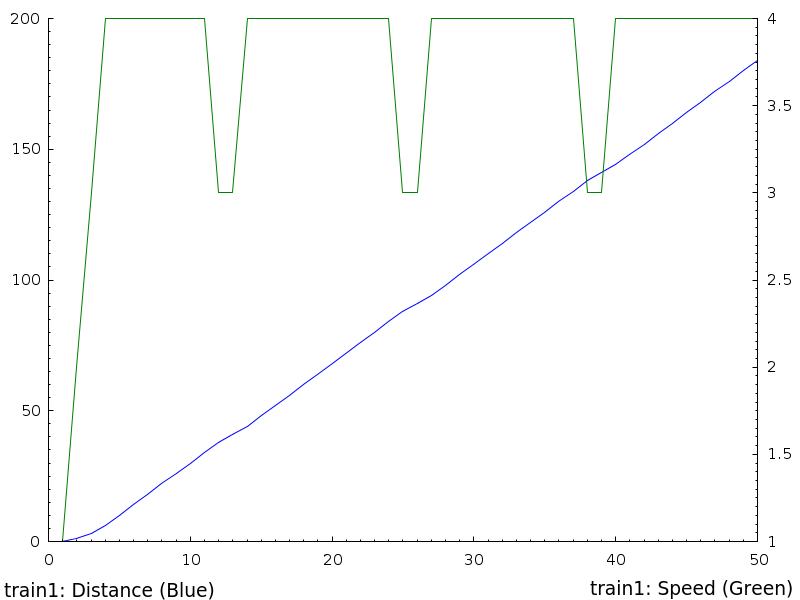
\includegraphics[scale=0.5]{t1graph.png}
\end{center}
\caption{A graph comparing the distance and speed of train1}
\end{figure}

\begin{figure}
\begin{center}
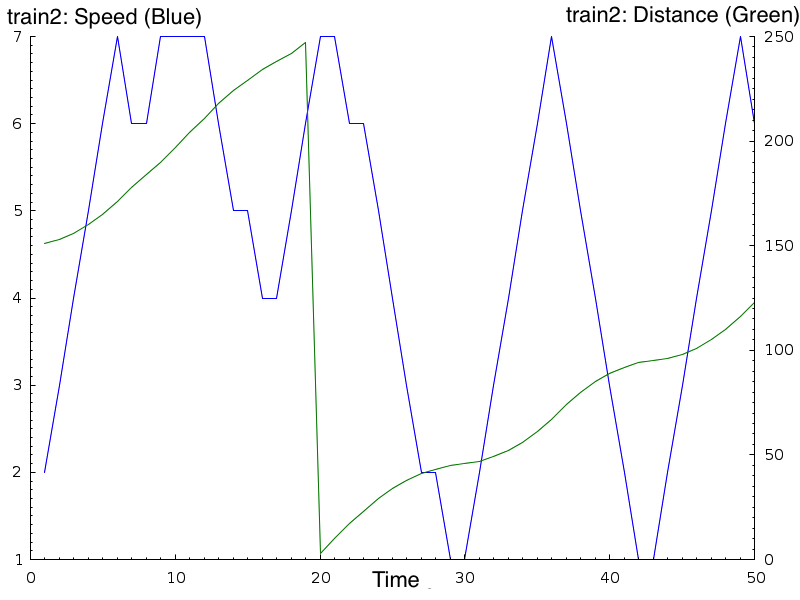
\includegraphics[scale=0.64]{t2graph.png}
\end{center}
\caption{A graph comparing the distance and speed of train2}
\end{figure}

\begin{figure}
\label{t1t2graph}
\begin{center}
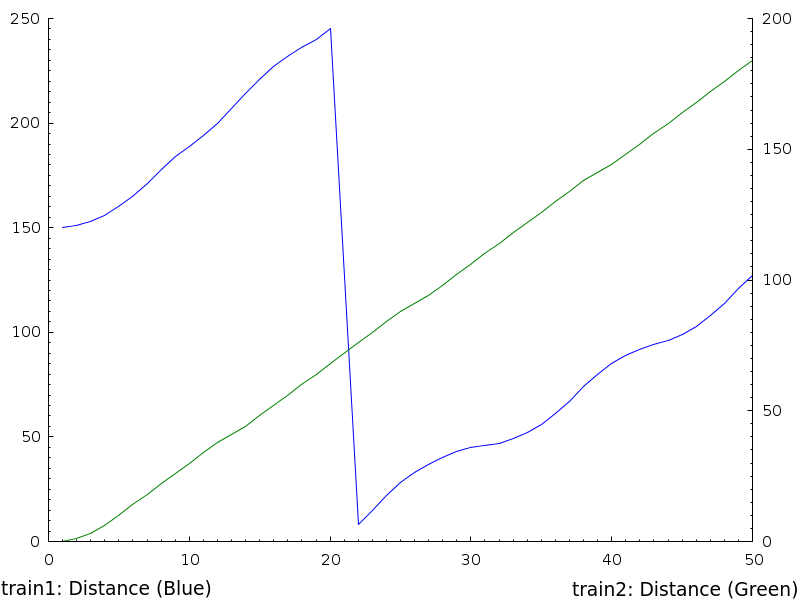
\includegraphics[scale=0.64]{t1t2graph.png}
\end{center}
\caption{A graph comparing the distances of train1 and train2}
\end{figure}

In fig \ref{t1t2} we see that train2 never enters the same track segment as train1.

\section{The Maude Linear Temporal Logic Model Checker}
The Real Time Maude system includes a model checker for linear temporal logic \cite{ES00}.  This is a useful automatic tool which allows for the verification and analysis of real time systems. In addition to the positive verification results in which a safety property holds,  the system produces, in the case of a negative verification result, a counter example trace which shows the. In the following we shall present formal definitions for linear temporal logic and the model checking problem for formulae in this logic.

 

\section{Model Checking the European Rail Traffic Management System}
In the following section we will demonstrate an approach to apply the Real Time Maude LTL model checker to verify the Real Time Maude specification described previously.
Firstly we shall define the property we want to check in the Real Time Maude system. To do this we have to define a satisfaction relation which describes what it means for the property to hold in a state of the system we are checking.  The property we shall consider in this case is that the moment authorities of two trains in system do not overlap. Logical property we define identifies the individual trains using their object identifiers and then computes whether or not an over lap has occurred using a boolean formula.  We shall show that it is possible to verify this property over a time period large enough for all normal behaviours of the system to occur. 

\subsection*{Defining a Satisfaction Relation}
The syntax of the properties for which we are going to check using the LTL model checker are defined separately from the semantics in terms of a satisfaction relation.
We shall now describe how to define the behaviour of the satisfaction relation for a given system and property as a Real Time Maude specification. The satisfaction relation itself is predefined in a specification as an operation which takes a State and a property which is of type Prop and computes a boolean. Maude defines the satisfaction relation $\models$ in the following:
\medskip

\begin{lstlisting}[caption =  The Maude Satisfaction module, label =code:satisfaction ]
  fmod SATISFACTION is  
    protecting BOOL .  
    sorts State Prop .  
    op _|=_ : State Prop -> Bool [frozen] .  
  endfm
\end{lstlisting}
\medskip
The sorts \texttt{State} and \texttt{Prop} are undefined as is the behaviour of $\models$. It is left to the user of the model checker to define the behaviour for their own purposes. The standard way to define predicates which refer to a given object is by matching object identifiers.

We can check that a train is in a specific state as follows:
\begin{lstlisting}[caption = The constant speed property]
ops train-cons : Oid -> Prop [ctor] .
eq {REST < O1 : Train | state : cons >} |= train-cons(O1') 
   = (O1 == O1') . 
\end{lstlisting}
This predicate holds if there is a train in t he configuration with object identifier O1' and a state cons. 

We can check that a train has a certain speed as follows:
\begin{lstlisting}[caption = The speed property]
op train-s : Oid Nat -> Prop [ctor] .
eq {REST < O1 : Train | speed : N1 >} |= train-s(O1',N1') = 
   (N1 == N1') and (O1 == O1') .
\end{lstlisting}

Here the natural number N1 in the train object is matched with N1' in the predicate train-s.
The main movement authority that we want to check is that the movement authorities of two trains does not over lap.
To do this we define a Property nomaoverlap(O1,O2) of type \texttt{Oid Oid -> Prop [ctor]} as follows: 

\begin{lstlisting}
eq {REST < O1 : Train |  dist : D1 , ma : M1 > 
   < O2 : Train |  dist : D2 , ma : M2 >} |= nomaoverlap(O1',O2') = 
   (O1 == O1') and (O2 == O2') and noolap(D1,M1,D2,M2) .
\end{lstlisting}
Here we have matched two object identifiers and natural numbers and called a boolean function \texttt{noolap} on those variables. This definition features an external operation which computes a boolean depending on whether a set of inequalities are satisfied. 

\begin{lstlisting}[caption = The no overlap operation]
eq noolap(D1,M1,D2,M2) = 
   ((D1 < M1) and (M1 < D2) and (D2 < M2)) or 
   ((D2 < M2) and (M2 < D1) and (D1 < M1)) or 
   ((D1 < M1) and (M2 < D1) and (M1 < D2)) or 
   ((D2 < M2) and (M1 < D2) and (M2 < D1) )  .  
\end{lstlisting}

This external operation encodes the 4 possible combines of movement authorities and trains in which the movement authorities do not over lap.  The first case is that train one is behind its movement authority which is behind the second train which itself is behind the movement authority. The second case is the reverse of the first case. In the third and fourth cases  one of the trains is behind its movement authority and the other is towards the end of the track and has its movement authority extended into the initial segment at the beginning of the track.

\subsection{Execution of The LTL Model Checker}
\textbf{Note: do we want to describe and verify other safety conditions here?}
We shall now describe the execution of the LTL model checker in Real Time Maude. This is done using the mc command with some initial state of type system, a satisfaction relation, the LTL formula to be checked and an optional time. The satisfaction relation can be either $\models_u$ for un-timed model checking for which time is not specified or $\models_t$ for which the optional time is specified.

The Real Time Maude LTL model checker is then called using the following command:

\begin{center}
\texttt{(mc initialstate2 |=t [] nomaoverlap(train1,train2) in time <= 30 .)}
\end{center}
The command states that we are applying timed model checking to check that it is globally true that the movement authorities of the trains do not over lap at all moments in time less than or equal to 30. This results in the following output from Real Time Maude which indicates that the property was succesfully verified in 3 minutes and 22 seconds taking the system approximately 140 million rewrites.
\begin{lstlisting}[caption = No overlapping movement authorities model checking result]
rewrites: 138889387 in 179663ms cpu 
(202024ms real) (773054 rewrites/second)

Model check initialstate2 |=t[]nomaoverlap(train1,train2)in 
MODEL-CHECK-ERTMS8 in time <= 30 
with mode deterministic time increase

Result Bool :
  true
\end{lstlisting}

Unfortunately the Real Time Maude LTL model checker can not detect the congruence between difference configurations of control system. Therefore the state space is infinite and it is impossible to do untimed model checking on the above model checking problem. It is however possible to do timed model checking within a reasonable time limit that allows for all behaviours of the system to be verified.

\section{Conclusion}
 We have presented the first attempt at modelling and verifying the combined ERTMS and interlocking system.
\subsection*{Future Work}
There are numerous ways in which our model can be extended. One of the biggest problems facing engineers when developing the ERTMS system is time and how it affects the transition of messages with delays often occurring. This could be easily be modelled following the work \cite{PO07} where delays are modelled in the communications between nodes of a wireless sensor network. Currently our trains have a jerky behaviour in terms of speed, breaking and accelerating in rapid succession there are several other behaviours that trains exhibit in real life that we have not captured in our model. Trains have the ability to coast where the engine in not powering the train but the brakes are not active which is used for several purposes. To save energy coasting and accelerating are often combined to hold the train at max speed. The trains may also coast before breaking when reaching the end of a movement authority.

Currently the track is closed and trains are capable of looping round the track giving it an infinite state space. Opening up the track with an entrance and exit would provide the opportunity to model the hand over part of the protocol where new trains must register with the RBC on entering the track and then de-register upon leaving. This opening of the track would also finitise the state space possibly allowing for un-timed model checking to take place. This example could then be extended by increasing the complexity of the track further and then modelling routes and points. This would allow for the checking of a further safety conditions that states no train has a movement authority over a point in locked in the wrong direction or a moving point.

The RBC has the possibility to pre-emptively grant movement authorities to trains without them requesting it in the case that a train is on a route which contains free sections of track behind a movement authority.  The trains could also request movement authorities before the point at which we reach the braking point.

\thesischapter{Simulating and Verifying the European Rail Traffic Management System Using Real Time Maude}{SImulating and Verifying ERTMS Using Real Time Maude}\label{chapter:verifyertms}\label{chap:verifyertms}
In the following we describe how the Real Time Maude tool can be used to analyse the performance and safety of the ERTMS system by both simulation and verification using the Maude LTL model checker (The modelling of ERTMS in Real Time Maude was describe in Chapter \ref{chap:modelertms}).  We begin by presenting the simulation of the pentagon example which demonstrates a situation where a slow train is held up by a faster train. Secondly we look at applying model checking to both the pentagon example and the junction example. The safety properties verified for the pentagon example relate to the safety condition "The movement authorities of the two trains do not overlap" whilst the properties for the junction example relate to the safety condition "The point does not move when it is in a trains movement authority". We also modify the pentagon example to use more realistic distances with a track segment length of 25000, segment length of 5000 and train speeds of 70 and 120.  We then apply the LTL model checker and verify this example so that a comparison can be performed between the two pentagon examples in terms of verification difficulty.

It is stated by its developers that Real Time Maude is not first and foremost a verification tool. This is due to some inherent limitations in LTL-model checking that hinder the verification of infinite state systems. We have, as in the sensor network example \cite{PO07}, only model checked a portion of the state space for the pentagon. This is however enough to have confidence in the correctness of the system with respect to a given safety condition. A larger portion of the state space could be model checked by removing non-determinism from the model making it more concrete. This has been done in the junction example where the radio block processor is modified in such a way that it processes movement authorities in one time step.


\section{Simulating The Behaviour of ERTMS}

We will now see how this executable specification can be used to simulate and analyse the perofrmance of the modelled system. Simulation of the system up to a given time $n$ is achieved by rewriting the initial state of the system to each of the intermediate time steps $0 \ldots n$. A simple Haskell program has been written that can parse the output of each step, extract the relevant data and then plot a graph.

We use an initial state containing two trains one of which is slower (train1) than the other (train2), an interlocking and a radio block processor. The faster train will eventually catch up with the slow train and it waits for that train to clear all successive track segments before proceeding. The trains start at positions on opposing sides of the track with train1 starting at 0 and train2 starting at 150. The RBC and the interlocking are both initialised with the trains in these positions. In Maude this initial state is modelled as follows. Firstly, we define the initial states of the component objects individually:

\begin{lstlisting}[caption = The initial interlocking state in Maude]
 eq initialintstate2 = < inter1 : Inter | state : idle, 
                         reqid : 0, t0 : true, 
                         t1 : false, t2 : false, 
                         t3 : true, t4 : false > .
\end{lstlisting}

The  interlocking is initially idle, the request variable is set to zero, the track segments containing trains are set to true and the remaining track segments are set to false.

\begin{lstlisting}[caption = The initial RBC state in Maude]
 eq initialrbcstate2 = < rbc1 : RBC | state : rbcidle, 
                         lasttrain : train1,  
                         ma : (train1 |-> 49, train2 |-> 199), 
                         pos : (train1 |-> 0, train2 |-> 150), 
                         curreq : empty > .
\end{lstlisting}

Like the interlocking, the RBC is also initially idle. Since the lasttrain variable has not effect in this state and will be set in any successive control flow we simply set it to be train1. The movement authorites  and positions of the trains are set within the ma and pos mapping respectively and the current request is empty.  

\begin{lstlisting}[caption = The intital state of train1 in Maude]
 eq initialtrainstate1 = < train1 : Train | state : acc,  dist : 0, 
                           speed : 1, ac : 1, ma : 49, 
                           tseg : 0, maxspeed : 4 > .
\end{lstlisting}
We set the train1 to be accellerating initally with a distance and speed of 0 its movement authority is 49, it is in the 0 track segment and has a maxspeed of 4. 

\begin{lstlisting}[caption = The intial state of train2 in Maude]
eq initialtrainstate2  = < train2 : Train | state : acc, dist : 150, 
                           speed : 1, ac : 1, ma : 199,
                           tseg : 3, maxspeed : 7 > .
\end{lstlisting}
Like train1, train2 is also accellerating initially and has a speed of 0.  Unlike train1 it has a distance of 150, a movement authority of 199, it is in the 4th track segment number 3 and has a maxspeed of 4. Both trains have an accelleration of 1. 

Using these initial states for the individual objects we can form the initial state for our pentagon example using the following command:
\begin{lstlisting}
 eq initialstate2 = {initialtrainstate1 initialtrainstate2 
                         initialintstate2  initialrbcstate2} . 
\end{lstlisting}
The operation \texttt{initialstate2} is of type \texttt{System} and contains a \texttt{Configuration} consisting of the initial states of train1, train2, the rbc and the interlocking. This initial state forms a model of ERTMS which we can simulate using Real Time Maude to rewrite it to a state after a set number of time steps. The model of ERTMS is executed using the following command:
\begin{center}
\texttt{(trew initialstate2 in time $\leq$ 50 .)}
\end{center}

In the resulting output at time 50 both of the trains have moved a considerable distance with train1 (See line 9 of Code Listing \ref{cl:initialstate2rewrite}.) moving to distance 184 and train2 moving to distance 128. Both trains have also requested and received new movement authorities.
 
\begin{lstlisting}[caption = The result of rewriting initialstate2 for 50 time steps, label = cl:initialstate2rewrite]
Result ClockedSystem :
  {< inter1 : Inter | reqid : 3,state : idle,
     t0 : false,t1 : false,t2 : true,
     t3 : true,t4 : false > 
   < rbc1 : RBC | curreq : train2,lasttrain : train2,
     ma : (train1 |-> 199, train2 |-> 149),
     pos : (train1 |-> 180, train2 |-> 122),
     state : rbcidle > 
   < train1 : Train | ac : 1,dist : 184,ma : 199,maxspeed : 4,
    speed : 4,state : cons,tseg : 3 > 
   < train2 : Train | ac : 1,dist : 128,ma :
    149,maxspeed : 7,speed : 5,state : break,tseg : 2 >} in time 50
\end{lstlisting}

\begin{figure}
\label{t1graph}
\begin{center}
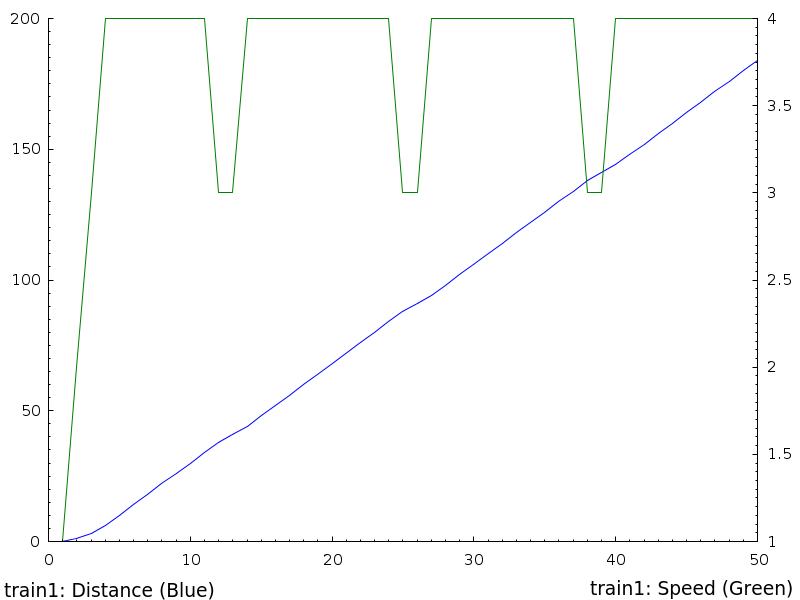
\includegraphics[scale=0.5]{t1graph.png}
\end{center}
\caption{A graph comparing the distance and speed of train1}
\end{figure}

\begin{figure}
\label{t2graph}
\begin{center}
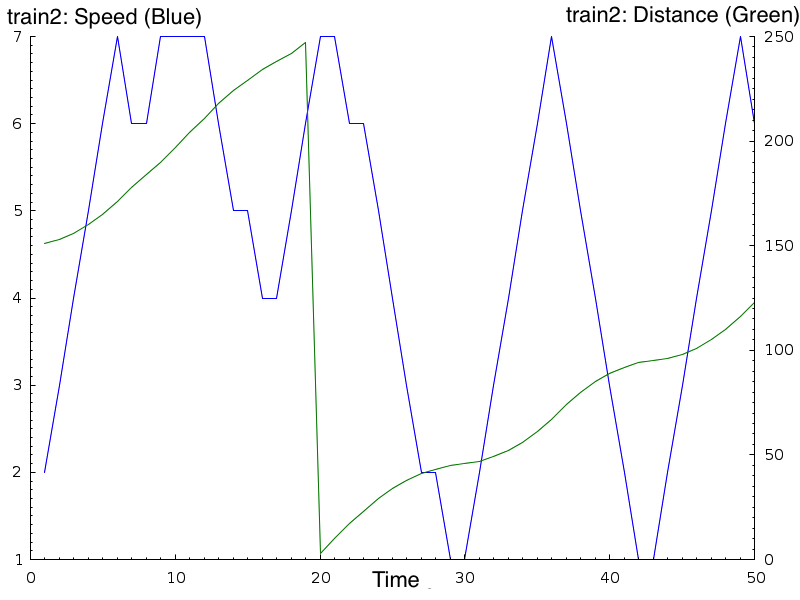
\includegraphics[scale=0.5]{t2graph.png}
\end{center}
\caption{A graph comparing the distance and speed of train2}
\end{figure}

\begin{figure}
\label{t1t2graph}
\begin{center}
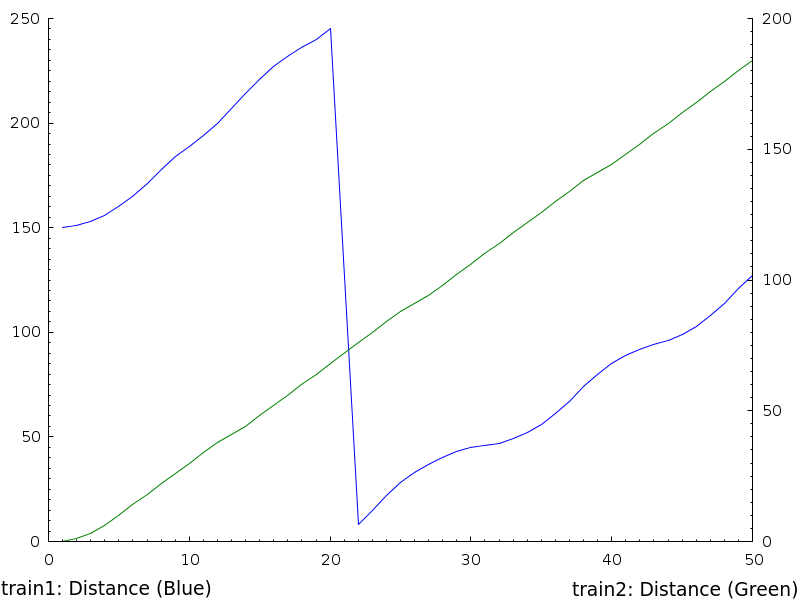
\includegraphics[scale=0.5]{t1t2graph.png}
\end{center}
\caption{A graph comparing the distances of train1 and train2}
\end{figure}

The first graph (See fig \ref{t1graph}.) shows the speed and distance of train1 over time. The train spends the majority of its time at max speed however there is a slight decrease in speed when a movement authority is requested. The distance of the train increases in roughly a linear fashion. The second graph (See fig \ref{t2graph}.) shows the speed and distance of train2 over time. The train brakes repeatedly and at one position comes to a complete stop as it waits for the slower train to progress and exit its current track segment. The distance time graph shows this stop/start behaviour through a wavey appearence. The final graph (See fig \ref{t1t2graph}.) shows that there is a consistent distance between the two trains of at least one track segment. Due to the discretisation of time we have had to favour braking over accelerating in order for the train to stop behind its movement authority. The speed of the train decreases on a transition from accelerating or full speed states to a braking state but does not increase speed immediatley on a transition from a braking to accelerating state. This behaviour can be see in the speed graph for train2 (See fig \ref{t2graph}.) where there are several sharp peaks where the max speed has only been in place for one time step. In contrast when the train transitions from braking to accelerating there is always a flat section of constant speed. These flat sections of constant speed also occur when the train is braking and the train jumps back into the accelerating state for one time step to ensure the train brakes as closely to the end of movement authority as possible.


\section{The Maude Linear Temporal Logic Model Checker}
The Real Time Maude system employs the Maude LTL Model Checker on-the-fly LTL model checker for \cite{ES00} verification purposes.  This is a useful automatic tool which allows for the verification and analysis of real time systems. In addition to the positive verification results in which a safety property holds,  the system produces, in the case of a negative verification result, a counter example trace which describes how the error occured from the initial state of the system.

 

\section{Model Checking the European Rail Traffic Management System}
In the following section we will demonstrate an approach to apply the Real Time Maude LTL model checker to verify the Real Time Maude specification described previously.
Firstly we shall define the property we want to check in the Real Time Maude system. To do this we have to define a satisfaction relation which describes what it means for the property to hold in a state of the system we are checking.  The property we shall consider in this case is that the moment authorities of two trains in system do not overlap. Logical property we define identifies the individual trains using their object identifiers and then computes whether or not an over lap has occurred using a boolean formula.  We shall show that it is possible to verify this property over a time period large enough for all normal behaviours of the system to occur. 

\subsection*{Defining a Satisfaction Relation}
The syntax of the properties for which we are going to check using the LTL model checker are defined separately from the semantics in terms of a satisfaction relation.
We shall now describe how to define the behaviour of the satisfaction relation for a given system and property as a Real Time Maude specification. The satisfaction relation itself is predefined in a specification as an operation which takes a State and a property which is of type Prop and computes a boolean. Maude defines the satisfaction relation $\models$ in the following:
\medskip

\begin{lstlisting}[caption =  The Maude Satisfaction module, label =code:satisfaction ]
  fmod SATISFACTION is  
    protecting BOOL .  
    sorts State Prop .  
    op _|=_ : State Prop -> Bool [frozen] .  
  endfm
\end{lstlisting}
\medskip
The sorts \texttt{State} and \texttt{Prop} are undefined as is the behaviour of $\models$. It is left to the user of the model checker to define the behaviour for their own purposes. The standard way to define predicates which refer to a given object is by pattern matching object identifiers. We have added general rules to deal with terms containing the operations \texttt{delta} and \texttt{trackseg}. In both cases the operation is ignored and the property is checked on the term without the operations.

\begin{lstlisting}[caption = Rewriting rules to deal with delta and trackseg operations]
var P : Prop .
eq {delta(REST)REST2} |= P = {REST REST2} |= P .
eq {trackseg(REST)REST2} |= P = {REST REST2} |= P .
\end{lstlisting}

\subsection*{Checking the  Correctness of the Specification}

We have applied model checking to check several fundemental correctness properties of the pentagon examples behaviour. We begin by showing that it is not possible for a train to exceed its max speed. We formulate this as a model checking problem over the pentagon example.  We can check that a train has a certain speed as follows:

\begin{lstlisting}[caption = The speed property]
op train-s : Oid Nat -> Prop [ctor] .
eq {REST < O1 : Train | speed : N1 >} |= train-s(O1,N1') = 
   (N1 == N1')  .
\end{lstlisting}

Here the natural number N1 in the train object is matched with N1' in the predicate train-s. This can be used to that train1 does not exceed its maximum speed in any state in the pentagon  example that is reachable in 30 time steps using the following command:

\begin{center}
\texttt{(mc initialstate2 |=t  ~(<> train-s(train1,5)) in time <= 100 .)}
\end{center}

The resulting output from the model checker shows that the property has been proven true in 230 seconds:

\begin{lstlisting}
rewrites: 66202099 in 229900ms cpu (229901ms real) 
(287960 rewrites/second)
Model check initialstate2 |=t ~ <> train-s(train1,5)
in MODEL-CHECK-ERTMS8 in time
  <= 100 with mode deterministic time increase

Result Bool : true
\end{lstlisting}

We will now show that the train is always at the correct speed for the cons and stopped states. This is formulated using two properties. We can check that a train is in a specific state, in this case the cons state, as follows:

\begin{lstlisting}[caption = The cons state property]
ops train-cons : Oid -> Prop [ctor] .
eq {REST < O1 : Train | state : S >} |= train-cons(O1) 
   =  S == cons . 
\end{lstlisting}


This predicate holds if there is a train in the configuration with object identifier O1 and a state cons. 

We can use these two properties and others formulated in a similar fashion to formulate model checkng properties which can be used check the correctness of our modelling approach. We can define three safety conditions, one that states "train1 is in the cons state if and only it is at its max speed". The second states "if the speed of train1 is zero then it is either in the cons, stop or acc states and if the train is in the stop state then its speed is zero". The final states "it is not the case that there exists a state in which the speed of train1 is 5" (train1 has a max speed of 4). 

\begin{lstlisting}
Correct1 := (mc initialstate2 |=t  
  ~(<> train-s(train1,5)) in time <= 100 .)
Correct2 := (mc initialstate2 |=t 
  [] (train-s(train1,4) => train-cons(train1)) /\ 
     (train-cons(train1) => train-s(train1,4))  
  in time <= 100 .)
Correct3 := (mc initialstate2 |=t [] ((train-s(train1,0) => 
  (train-stop(train1) \/ train-brake(train1) \/ train-acc(train1))) 
   /\ (train-stop(train1) => train-s(train1,0))) in time <= 100 .)
\end{lstlisting}

\subsection*{Defining "No Overlapping Movement Authorities"}
We verifying the safety condition "The movment authorities of two trains do not overlap" by model checking three safety properties MA1, MA2 and MA3 that correspond to checking the different possible safe positions over movement authorities and trains on the track. To do this we define a satisfaction relation for two Maude operations of type $\mathbf{Prop}$ which capture each of these safety properties. The first of which can be seen below:

\begin{lstlisting}
eq {REST < O1 : Train |  dist : D1 , ma : M1 > 
   < O2 : Train |  dist : D2 , ma : M2 >} |= nomaoverlap1(O1',O2') = 
   (O1 == O1') and (O2 == O2') and noolap1(D1,M1,D2,M2) .
\end{lstlisting}

Here we have matched two object identifiers and natural numbers and called a boolean function \texttt{noolap} on those variables. This definition features an external operation which computes a boolean depending on whether a set of inequalities are satisfied. The three sets of inequalities corresponding to the three safety properties are defined below:

\begin{lstlisting}[caption = The no overlap operations]
eq noolap1(D1,M1,D2,M2) = 
    (D1 <= M1) and (D2 <= M2) implies ((M1 <  D2) or (M2 < D1)) .  
eq noolap2(D1,M1,D2,M2) = 
    ((M1 < D1) and (D2 <= M2)) implies (M2 < D1 and M1 < D2) .
eq noolap3(D1,M1,D2,M2) = 
    ((M2 < D2) and (D1 <= M1)) implies (M1 < D2 and M2 < D1) .

\end{lstlisting}

There are four possible combinations of trains and movement authorities.  The first case is that train one is behind its movement authority which is behind the second train which itself is behind the movement authority. The second case is the reverse of the first case. In the third and fourth cases  one of the trains is behind its movement authority and the other is towards the end of the track and has its movement authority extended into the initial segment at the beginning of the track.


\subsection*{Defining "A Point Does Not Move"}
We formalise the safety property "a point does not move when it is in a movement authority" as two safety conditions. The first states that it is globally true that if the point is in the movement authority of train1 then the point is set to normal. The second states that it is globally true that if the point is in the movement authority of train2 then the point is set to reverse. These two safety conditions were formalised using 3 Maude operations of type $\mathbf{Prop}$, $\mathbf{pointma}$ is used to compute whether the point is in the movement authority of a train, $\mathbf{pointnormal}$ and $\mathbf{pointreverse}$ cause the satisfaction relation to hold if the point is in the position corresponding to the property. 

\begin{lstlisting}
  eq { REST  < O1 : Train |  dist : D1 , ma : M1 > } |= pointma(O1) 
      =  ptma(D1, M1)  .
  eq { REST   < O1 : Inter | p1n : B >  } |= pointnormal = B .
  eq { REST   < O1 : Inter | p1r : B >  } |= pointreverse = B .
\end{lstlisting}

\subsection{Execution of The LTL Model Checker}

We shall now describe the execution of the Maude LTL model checker in Real Time Maude. This is done using the mc command with some initial state of type system, a satisfaction relation, the LTL formula to be checked and an optional time. The satisfaction relation can be either $\models_u$ for un-timed model checking for which time is not specified or $\models_t$ for which the optional time is specified.

The Maude LTL model checker is then called using the following command:

\begin{center}
\texttt{(mc initialstate2 |=t [] nomaoverlap1(train1,train2) in time <= 100 .)}
\end{center}
The command states that we are applying timed model checking to check that it is globally true that the movement authorities of the trains do not over lap at all moments in time less than or equal to 100. This results in the following output from Real Time Maude which indicates that the property was succesfully verified in 1 minutes and 32 seconds taking the system approximately 76 million rewrites.
\begin{lstlisting}[caption = No overlapping movement authorities model checking result]
rewrites: 76099490 in 91776ms cpu (91776ms real) 
(829187 rewrites/second)
Model check initialstate2 |=t[]nomaoverlap1(train1,train2)
in MODEL-CHECK-ERTMS8
   in time <= 100 with mode deterministic time increase

Result Bool : true
\end{lstlisting}

Unfortunately the Maude LTL model checker can not detect the congruence between difference configurations of control system. Therefore the state space is infinite and it is impossible to do untimed model checking on the above model checking problem for the pentagon example. It is however possible to do timed model checking within a reasonable time limit that allows for all behaviours of the system to be verified. The junction example does not suffer from this problem as the state space is finite and in addition, it has additional mechanisms to remove non-determinism from the model which dramatically cuts down on the state space.

The following command is used to model check the safety property P1 for the junction example.

\begin{lstlisting}
(mc initialstate1 |=u [] (pointma(train1) => pointnormal)  .)
\end{lstlisting}

\section{Results}
The following table presents the times taken to verify the 4 safety properties MA1, MA2, MA3, P1 and P2:
\begin{center}
\begin{tabular}{c | c | c} 
Safety Condition & Time Steps Checked & Time to Solve  \\ \hline
Correct1 & 100 & 229.400 s\\
Correct2 & 100 & 249.784s\\
Correct3 & 100 & 225.556s\\
MA1 (Pentagon)& 100 & 91.756s  \\
MA2 (Pentagon)& 100 &129.335s \\ 
MA3 (Pentagon)& 100 &148.032s \\
P1 (Junction)& untimed &7.488s \\
P2 (Junction)& untimed & 6.636s \\
\end{tabular}
\end{center}

The removal of non-determinism from the pentagon example has made untimed model checking possible. Prior to the \texttt{nondelta} operation being added the safety properties could only be checked for the first 30 time steps of the system.

The no overlapping movement authorities safety property was verified using time bounded model checking over the modified pentagon example containing realistic speeds and distances. The following table shows how the difficulty of the model checking problem increases with search depth:

\begin{center}
\begin{tabular}{c | c | c} 
Safety Condition & Time Steps Checked & Time to Solve  \\ \hline
MA1 (Realistic Pentagon) & 30 & 25.265s \\
MA1 (Realistic Pentagon) & 40 & 36.414s \\
MA1 (Realistic Pentagon) & 50 & 49.201s \\
MA1 (Realistic Pentagon) & 60 & 62.126s \\
MA1 (Realistic Pentagon) & 70 & 79.948s \\
\end{tabular}
\end{center}

Even though the Real Time Maude system is unable to performed untimed model checking on this example it can still perform bounded model checking of a large enough portition of the state space for us to be

\section{Conclusion}
 We have presented the first attempt at modelling and verifying the combined ERTMS and interlocking system.
\subsection*{Future Work}
There are numerous ways in which our model can be extended. One of the biggest problems facing engineers when developing the ERTMS system is time and how it affects the transition of messages with delays often occurring. This could be easily be modelled following the work \cite{PO07} where delays are modelled in the communications between nodes of a wireless sensor network. Currently our trains have a jerky behaviour in terms of speed, breaking and accelerating in rapid succession there are several other behaviours that trains exhibit in real life that we have not captured in our model. Trains have the ability to coast where the engine in not powering the train but the brakes are not active which is used for several purposes. To save energy coasting and accelerating are often combined to hold the train at max speed. The trains may also coast before breaking when reaching the end of a movement authority.


\begin{comment}
Currently the track is closed and trains are capable of looping round the track giving it a very large state space due to number of possible combinations of train location and speed. Opening up the track with an entrance and exit would provide the opportunity to model the hand over part of the protocol where new trains must register with the RBC on entering the track and then de-register upon leaving. This would  This example could then be extended by increasing the complexity of the track further and then modelling routes and points. This would allow for the checking of a further safety conditions that states no train has a movement authority over a point in locked in the wrong direction or a moving point.
\end{comment}

This next challenge would be to verify to verify some real world track layouts as would be controlled by the ERTMS system on its implementation. \textbf{Note to self: write some paragraph here to replace the above. something about different track layouts that can be verified.}


The RBC has the possibility to pre-emptively grant movement authorities to trains without them requesting it in the case that a train is on a route which contains free sections of track behind a movement authority.  The trains could also request movement authorities before the point at which we reach the braking point.



\bibliographystyle{alpha}
\bibliography{lit.bib}

\appendix


\thesischapter{Proof Systems}

\section{Gentzen's Sequent Calculus}
These rules and propositions were taken from St{\aa}lmarck \cite{GS00}.
\label{def:sequent}
\begin{mydef}[Sequent]
Every line in sequent calculus proof is called a sequent and takes the
following form. 

$$ A_1, \ldots , A_k \vdash B_1, \ldots ,B_l$$

In this text we are using the symbol $\vdash$ to represent the sequent arrow.
\footnote{The sequent arrow is sometimes represented using the symbol $\to$}
The following formula captures the meaning of the above sequent.

$$ \bigwedge_{i = 1}^{k} A_i \supset  \bigvee_{j-1}^l B_j$$

\end{mydef}
 
\medskip

Intuitively you can read a sequent as: If the conjunction of all of the $A_i$s
is true then one of the $B_j$s in the disjunction must be true.

\medskip

\begin{mydef}[Gentzen's Sequent Calculus PK] \hspace*{\fill} \\

Axiom
\bigskip
\begin{center}
$A \vdash A$
\end{center}

\bigskip

Structural Rules

\bigskip
\begin{center}


\AxiomC{$\Gamma \vdash \Delta $}
\LeftLabel{($Thinning$)}
\UnaryInfC{$\Gamma, \Theta \vdash \Delta, \Lambda $}
\DisplayProof \
\AxiomC{$\Gamma, A \vdash \Delta$}
\AxiomC{$\Gamma \vdash \Delta, A$}
\LeftLabel{($Cut$)}
\BinaryInfC{$\Gamma \vdash \Delta$}
\DisplayProof

\end{center}

\bigskip

Operational Rules

\bigskip
\begin{center}
\AxiomC{$\Gamma, A \vdash \Delta$}
\AxiomC{$\Gamma, B \vdash \Delta$}
\LeftLabel{($Or_L$)}
\BinaryInfC{$\Gamma, A \vee B \vdash \Delta$}
\DisplayProof \
\AxiomC{$\Gamma \vdash \Delta, A,B$}
\LeftLabel{($Or_R$)}
\UnaryInfC{$\Gamma \vdash \Delta , A \vee B$}
\DisplayProof

\end{center}

\smallskip

\begin{center}

\AxiomC{$\Gamma, A, B \vdash \Delta$}
\LeftLabel{($And_L$)}
\UnaryInfC{$\Gamma, A \wedge B \vdash \Delta$}
\DisplayProof \
\AxiomC{$\Gamma \vdash \Delta, A$}
\AxiomC{$\Gamma \vdash \Delta, B$}
\LeftLabel{($And_R$)}
\BinaryInfC{$\Gamma, \vdash  \Delta, A \wedge B$}
\DisplayProof

\end{center}

\smallskip

\begin{center}

\AxiomC{$\Gamma \vdash \Delta, A$}
\AxiomC{$\Gamma , B \vdash \Delta$}
\LeftLabel{($Imp_L$)}
\BinaryInfC{$\Gamma, A \to B \vdash \Delta$}
\DisplayProof \
\AxiomC{$\Gamma ,A \vdash \Delta , B$}
\LeftLabel{$(Imp_R)$}
\UnaryInfC{$\Gamma \vdash \Delta, A \to B$}
\DisplayProof


\end{center}

\smallskip

\begin{center} 

\AxiomC{$\Gamma \vdash \Delta , A$}
\LeftLabel{$(Neg_L)$}
\UnaryInfC{$\Gamma, \neg A \vdash \Delta$}
\DisplayProof \
\AxiomC{$\Gamma , A \vdash \Delta$}
\LeftLabel{$(Neg_R)$}
\UnaryInfC{$\Gamma \vdash \Delta, \neg A$}
\DisplayProof


\end{center}

\smallskip

\end{mydef}

\medskip

\begin{proposition}[Sub-formula Principle]
If a PK-proof P does not contain any application of the cut rule, then
All of the formulas occurring in  P must be a sub-formula of some
formula in the end sequent of P.
\end{proposition}

\medskip

Having the \textit{sub-formula principle} allowed St{\aa}lmarck to place bounds on the
size of proofs created by his algorithm.

\medskip

\begin{proposition}[Removing Thinning]
If we allow axioms of the form $\Gamma, A \vdash A, \Delta$ then it is
possible to remove the thinning rule as it is redundant and is no longer of
any use.

\end{proposition}

\medskip

Removing the thinning rule gives us a proof system that is essentially the
same as that by Kleene \cite{SK67}. This proof system has the advantage that it
is invertible i.e., if a sequent below the line of an inference is valid then
the sequents above the line are also valid.

\section{Smullyan's Semantic Tableaux}
The Analytic tableaux form a refutation proof system. You begin a proof by
assuming your propositional formula is false. Then a tree is constructed using
the rules. The formula is de-constructed into its constituent sub-formulae
using the rules \textit{And}, \textit{Not-Or} and \textit{Not-Impl}. Case
distinction on the formula is performed by the rules \textit{Or},
\textit{Not-And} and \textit{Impl}. The application of a case distinction rule
causes a branch to occur in the proof tree. If each branch of the tree contains a contradiction then the
formula is refuted.


\label{def:tableaux}
\begin{mydef}[Semantic Tableaux] \hspace*{\fill} \\
\begin{center}

\AxiomC{$A \wedge B$}
\LeftLabel{$(And)$}
\UnaryInfC{$A$}
\alwaysNoLine
\UnaryInfC{$B$}
\DisplayProof \
\AxiomC{$\neg(A \vee B)$}
\LeftLabel{$(Not\hyp{}Or)$}
\UnaryInfC{$\neg A$}
\alwaysNoLine
\UnaryInfC{$\neg B$}
\DisplayProof


\end{center}

\begin{center}

\AxiomC{$A \vee B$}
\LeftLabel{$(Or)$}
\UnaryInfC{$A | B$}
\DisplayProof \
\AxiomC{$\neg(A \wedge B)$}
\LeftLabel{$(Not \hyp{} And)$}
\UnaryInfC{$\neg A | \neg B$}
\DisplayProof


\end{center}

\begin{center}

\AxiomC{$A \to B$}
\LeftLabel{$(Impl)$}
\UnaryInfC{$\neg A | B$}
\DisplayProof \
\AxiomC{$\neg(A \to B)$}
\LeftLabel{$(Not \hyp{} Impl)$}
\UnaryInfC{$A$}
\alwaysNoLine
\UnaryInfC{$\neg B$}
\DisplayProof



\end{center}

\begin{center}

\AxiomC{$\neg \neg A$}
\LeftLabel{$(Not \hyp{} Not)$}
\UnaryInfC{$A$}
\DisplayProof \

\end{center}


\end{mydef}

\medskip

\section{Propagation Rules for St{\aa}lmarck's Tautology Checker}

In the following the proper rules used in St{\aa}lmarck's tautology checking
algorithm are presented from \cite{JN01}.

\label{sec:stalmarck}

\medskip

\begin{mydef}[Formula Equivalence Rules] \hspace*{\fill} \\
\begin{equation}
\AxiomC{}
\UnaryInfC{$P \equiv P$}
\DisplayProof \
\end{equation}

\begin{equation}
\AxiomC{$P \equiv Q$}
\UnaryInfC{$Q \equiv P$}
\DisplayProof \
\end{equation}

\begin{equation}
\AxiomC{$P \equiv Q$}
\AxiomC{$ Q \equiv R  $}
\BinaryInfC{$P \equiv R$}
\DisplayProof \
\end{equation}

\begin{equation}
\AxiomC{$P \equiv \bot$}
\UnaryInfC{$P' \equiv \top$}
\DisplayProof \
\end{equation}

\begin{equation}
\AxiomC{$P \equiv Q$}
\AxiomC{$ Q \equiv \top  $}
\BinaryInfC{$P \equiv \top$}
\DisplayProof \
\end{equation}

\begin{equation}
\AxiomC{$P \equiv Q$}
\AxiomC{$ Q \equiv \bot  $}
\BinaryInfC{$P \equiv \bot $}
\DisplayProof \
\end{equation}


\begin{equation}
\AxiomC{$P \equiv Q$}
\UnaryInfC{$P' \equiv Q'$}
\DisplayProof \
\end{equation}

\begin{equation}
\AxiomC{$P \equiv \top$}
\UnaryInfC{$P' \equiv \bot$}
\DisplayProof \
\end{equation}


\begin{equation}
\AxiomC{$P \equiv \top$}
\AxiomC{$Q \equiv \top$}
\BinaryInfC{$P \equiv Q$}
\DisplayProof \
\end{equation}


\begin{equation}
\AxiomC{$P \equiv \bot$}
\AxiomC{$Q \equiv \bot$}
\BinaryInfC{$P \equiv Q$}
\DisplayProof \
\end{equation}

\begin{equation}
\AxiomC{$P \equiv P'$}
\UnaryInfC{$\bot$}
\DisplayProof \
\end{equation}


\end{mydef}



\begin{mydef}[Propagation Rules]

Rules for conjunction

\begin{equation}
\AxiomC{$P \wedge Q \equiv \top$}
\UnaryInfC{$P \equiv \top$}
\DisplayProof \hspace*{30pt}
\AxiomC{$P \wedge Q \equiv \top$}
\UnaryInfC{$Q \equiv \top$}
\DisplayProof \
\end{equation}


\begin{equation}
\AxiomC{$P \wedge Q \equiv P'$}
\UnaryInfC{$P \equiv \top$}
\DisplayProof \hspace*{30pt}
\AxiomC{$P \wedge Q \equiv Q'$}
\UnaryInfC{$Q \equiv \top$}
\DisplayProof \
\end{equation}



\begin{equation}
\AxiomC{$P \wedge Q \equiv P'$}
\UnaryInfC{$Q \equiv \bot$}
\DisplayProof \hspace*{30pt}
\AxiomC{$P \wedge Q \equiv Q'$}
\UnaryInfC{$P \equiv \bot$}
\DisplayProof \
\end{equation}


\begin{equation}
\AxiomC{$P \equiv \top$}
\UnaryInfC{$P \wedge Q \equiv Q$}
\DisplayProof \hspace*{30pt}
\AxiomC{$Q \equiv \top$}
\UnaryInfC{$P  \wedge Q \equiv P$}
\DisplayProof \
\end{equation}

\begin{equation}
\AxiomC{$P \equiv \bot$}
\UnaryInfC{$P \wedge Q \equiv \bot$}
\DisplayProof \hspace*{30pt}
\AxiomC{$Q \equiv \bot$}
\UnaryInfC{$P  \wedge Q \equiv \bot$}
\DisplayProof \
\end{equation}

\begin{equation}
\AxiomC{$P \equiv Q$}
\UnaryInfC{$P \wedge Q \equiv P$}
\DisplayProof \hspace*{30pt}
\AxiomC{$P \equiv Q$}
\UnaryInfC{$P  \wedge Q \equiv Q$}
\DisplayProof \
\end{equation}

\begin{equation}
\AxiomC{$P \equiv Q'$}
\UnaryInfC{$P  \wedge Q \equiv \bot$}
\DisplayProof \
\end{equation}


Rules for disjunction


\begin{equation}
\AxiomC{$P \vee Q \equiv \bot$}
\UnaryInfC{$P \equiv \bot$}
\DisplayProof \hspace*{30pt}
\AxiomC{$P \vee Q \equiv \bot$}
\UnaryInfC{$ Q \equiv \bot$}
\DisplayProof \
\end{equation}

\begin{equation}
\AxiomC{$P \vee Q \equiv P'$}
\UnaryInfC{$P \equiv \bot$}
\DisplayProof \hspace*{30pt}
\AxiomC{$P \vee Q \equiv Q'$}
\UnaryInfC{$ Q \equiv \bot$}
\DisplayProof \
\end{equation}

\begin{equation}
\AxiomC{$P \vee Q \equiv P'$}
\UnaryInfC{$Q \equiv \top$}
\DisplayProof \hspace*{30pt}
\AxiomC{$P \vee Q \equiv Q'$}
\UnaryInfC{$ P \equiv \top$}
\DisplayProof \
\end{equation}

\begin{equation}
\AxiomC{$P \equiv \top$}
\UnaryInfC{$P \vee Q \equiv \top$}
\DisplayProof \hspace*{30pt}
\AxiomC{$Q \equiv \top$}
\UnaryInfC{$P \vee Q \equiv \top$}
\DisplayProof \
\end{equation}

\begin{equation}
\AxiomC{$P \equiv Q$}
\UnaryInfC{$P \vee Q \equiv P$}
\DisplayProof \hspace*{30pt}
\AxiomC{$P \equiv Q$}
\UnaryInfC{$P \vee Q \equiv Q$}
\DisplayProof \
\end{equation}

\begin{equation}
\AxiomC{$P \equiv Q'$}
\UnaryInfC{$P \vee Q \equiv \top$}
\DisplayProof \
\end{equation}

Rules for implication

\begin{equation}
\AxiomC{$P \to Q \equiv \bot$}
\UnaryInfC{$P  \equiv \top$}
\DisplayProof \
\end{equation}

\begin{equation}
\AxiomC{$P \to Q \equiv \bot$}
\UnaryInfC{$Q \equiv \bot$}
\DisplayProof \
\end{equation}

\begin{equation}
\AxiomC{$P \to Q \equiv P$}
\UnaryInfC{$P \equiv \top$}
\DisplayProof \
\end{equation}

\begin{equation}
\AxiomC{$P \to Q \equiv P$}
\UnaryInfC{$Q \equiv \top$}
\DisplayProof \
\end{equation}

\begin{equation}
\AxiomC{$P \to Q \equiv Q'$}
\UnaryInfC{$P \equiv \bot$}
\DisplayProof \
\end{equation}

\begin{equation}
\AxiomC{$P \to Q \equiv Q'$}
\UnaryInfC{$Q \equiv \bot$}
\DisplayProof \
\end{equation}

\begin{equation}
\AxiomC{$P \equiv \top$}
\UnaryInfC{$P \to Q \equiv Q$}
\DisplayProof \
\end{equation}

\begin{equation}
\AxiomC{$Q \equiv \top$}
\UnaryInfC{$P \to Q \equiv \top$}
\DisplayProof \
\end{equation}

\begin{equation}
\AxiomC{$P \equiv \bot$}
\UnaryInfC{$P \to Q \equiv \top$}
\DisplayProof \
\end{equation}

\begin{equation}
\AxiomC{$Q \equiv \bot$}
\UnaryInfC{$P \to Q \equiv P'$}
\DisplayProof \
\end{equation}

\begin{equation}
\AxiomC{$P \equiv Q'$}
\UnaryInfC{$P \to Q \equiv P'$}
\DisplayProof \hspace*{30pt}
\AxiomC{$P \equiv Q'$}
\UnaryInfC{$P \to Q \equiv Q$}
\DisplayProof \
\end{equation}

Rules for bi-implication

\begin{equation}
\AxiomC{$P \leftrightarrow Q \equiv \top$}
\UnaryInfC{$P \equiv Q$}
\DisplayProof \
\end{equation}

\begin{equation}
\AxiomC{$P \leftrightarrow Q \equiv \bot$}
\UnaryInfC{$P \equiv Q'$}
\DisplayProof \
\end{equation}

\begin{equation}
\AxiomC{$P \leftrightarrow Q \equiv P$}
\UnaryInfC{$Q \equiv \top$}
\DisplayProof \hspace*{30pt}
\AxiomC{$P \leftrightarrow  Q \equiv Q$}
\UnaryInfC{$P \equiv \top$}
\DisplayProof \
\end{equation}

\begin{equation}
\AxiomC{$P \leftrightarrow Q \equiv P'$}
\UnaryInfC{$Q \equiv \bot$}
\DisplayProof \hspace*{30pt}
\AxiomC{$P \leftrightarrow  Q \equiv Q'$}
\UnaryInfC{$P \equiv \bot$}
\DisplayProof \
\end{equation}

\begin{equation}
\AxiomC{$Q \equiv \top$}
\UnaryInfC{$P \leftrightarrow Q \equiv P$}
\DisplayProof \hspace*{30pt}
\AxiomC{$P \equiv \top$}
\UnaryInfC{$P \leftrightarrow  Q \equiv Q$}
\DisplayProof \
\end{equation}


\begin{equation}
\AxiomC{$Q \equiv \bot$}
\UnaryInfC{$P \leftrightarrow Q \equiv P'$}
\DisplayProof \hspace*{30pt}
\AxiomC{$P \equiv \bot$}
\UnaryInfC{$P \leftrightarrow  Q \equiv Q'$}
\DisplayProof \
\end{equation}


\begin{equation}
\AxiomC{$P \equiv Q$}
\UnaryInfC{$P \leftrightarrow Q \equiv \top$}
\DisplayProof \
\end{equation}


\begin{equation}
\AxiomC{$P \equiv Q'$}
\UnaryInfC{$P \leftrightarrow Q \equiv \bot$}
\DisplayProof \
\end{equation}

\end{mydef}

\medskip







\thesischapter{Concrete Railway Model} 


In this chapter we will present the work produced in attempt to provide a
concrete model of the railway (See Chapter 5).

\section{Railway Components}

In the following we have tried to model components of the railway with the intention
that they could be verified individually and then recombined into different
configurations.



 Track Segment 1:
 Node was used to model a straight piece of track. We have simplified the
 topological aspect somewhat
 since the track is generally set up for trains travelling in one direction. We
 have assumed that a train will not travel the wrong way down a track.

\begin{verbatim}

node Track_Segment1(TrainIn, RedLight, GreenLight, WhiteLight : bool)
returns(TrackOccupied, TrainOut, Crash: bool)
var



let

automaton
	initial state EMPTY

	let
	
			TrackOccupied = false; 
			TrainOut = false; 
			Crash = false;
	
	tel
	until
	if (TrainIn) restart OCCUPIED;
	
	state OCCUPIED
	let
		TrackOccupied = true ;
		TrainOut = false;
		Crash = false;
	 
	
	tel
	until
	if ((GreenLight or WhiteLight) and not RedLight) restart TRAINLEAVE;
	if (TrainIn) restart CRASH;
	
	state TRAINLEAVE
	let
	
		TrackOccupied = true;
		TrainOut = true;
		Crash = false;
	
	tel
	until
	if (TrainIn) restart CRASH;
	if (TrainOut) restart EMPTY;
	
	state CRASH
	let
	
		TrackOccupied = true;
		Crash = true;
		TrainOut = false;
	
	tel
	
	returns .. ;

tel

\end{verbatim}

 Track Segment 2:
 Originally we had modelled certain junctions using this component and
 of track using this component. 
 we decided however that we would like to capture all possible ways a train can move across a junction
 we therefore converted all track segments in junctions to using Track Segment 3.

\begin{verbatim}

node Track_Segment2(TrainIn1, TrainIn2, RedLight, GreenLight,
                    WhiteLight, PointsNorm, PointsRev : bool)
returns(TrackOccupied, TrainOut1, TrainOut2, Crash: bool)
var


let


automaton
	initial state EMPTY
	let
	
			TrackOccupied = false; 
			TrainOut1 = false; 
			TrainOut2 = false;
			Crash = false;
	
	tel
	until
	if (TrainIn1 or TrainIn2) restart OCCUPIED;
	
	state OCCUPIED
	let
		TrackOccupied = true;
		TrainOut1 = false;
		TrainOut2 = false;
		Crash = false;
		
	
	tel
	until
	if ((GreenLight or WhiteLight) and not RedLight) restart TRAINLEAVE;
	if (TrainIn1 or TrainIn2) restart CRASH;
	
	state TRAINLEAVE
	let
	
		TrackOccupied = true;
		TrainOut1 =  if (PointsRev) then true else false;
		TrainOut2 = if (PointsNorm) then true else false;
		Crash = false;
	
	tel
	until 
	if (TrainIn1 or TrainIn2) restart CRASH;
	if (TrainOut1 or TrainOut2) restart EMPTY;
	
	state CRASH
	let
	
		TrackOccupied = true;
		Crash = true;
		TrainOut1 = false;
		TrainOut2 = false;
	tel
	
	returns .. ;

tel

\end{verbatim}

 Track Segment 3: This is the node that was used to model junctions in the track. The just has
 been modelled in such a way that the direction of
 travel along with the points dictate how a train exits the track. 




\begin{verbatim}


node Track_Segment3(TrainIn1, TrainIn2, TrainIn3, RedLight, 
GreenLight, WhiteLight, PointsNorm , PointsRev : bool)
returns(TrackOccupied, TrainOut1, TrainOut2, TrainOut3 , Crash: bool)
var

Direction : bool;

let

Direction = false -> if (TrainIn1) then true else (if (TrainIn3) then false 
							else pre Direction); 

automaton
	initial state EMPTY
	let
	
			TrackOccupied = false; 
			TrainOut1 = false; 
			TrainOut2 = false;
			TrainOut3 = false;
			
			Crash = false;
	
	tel
	until
	if (TrainIn1 or TrainIn2 or TrainIn3) restart OCCUPIED;
	
	state OCCUPIED
	let
		TrackOccupied = true ;
		TrainOut1 = false;
		Crash = false;
		TrainOut2 = false;
		TrainOut3 = false;
	 
	
	tel
	until
	if ((GreenLight or WhiteLight) and not RedLight) restart TRAINLEAVE;
	if (TrainIn1 or TrainIn2 or TrainIn3) restart CRASH;
	
	state TRAINLEAVE
	let
	
		TrackOccupied = true;
		TrainOut1 = if (Direction) then false else true ;
		Crash = false;
		TrainOut2 = if (Direction and PointsRev) then true else false ;
		TrainOut3 = if (Direction and PointsNorm) then true else false;
	
	tel
	until
	if (TrainIn1 or TrainIn2 or TrainIn3) restart CRASH;
	if (TrainOut1 or TrainOut2 or TrainOut3) restart EMPTY;
	
	state CRASH
	let
	
		TrackOccupied = true;
		Crash = true;
		TrainOut1 = false;
		TrainOut2 = false;
		TrainOut3 = false;
	
	tel
	
	returns .. ;

tel


\end{verbatim}



\begin{verbatim}

node Route(RouteCall, RouteSet, PointsLocked,
 LightsSet, W_track_clear, G_track_clear: bool)
returns(RouteSelected, DrivePL, DriveG, DriveW, DriveR: bool) 
let
automaton
	initial state STATE1
	unless
	if (RouteCall) restart STATE2;
	let
	
		RouteSelected = false;
		DrivePL = false;
		DriveG = false;
		DriveW = false;
		DriveR = true;
	
	tel
	state STATE2
	unless
	if (not RouteSet) restart STATE1;
	if (RouteCall and PointsLocked and LightsSet) restart STATE3;
	let
	
	
		RouteSelected = false; 
		DrivePL = true;
		DriveG = if (W_track_clear and G_track_clear)
						then true
						else false;
		DriveW = if (W_track_clear and not G_track_clear)	
						then true
						else false;
		DriveR = if ( (W_track_clear and G_track_clear) 
                      or (W_track_clear and not G_track_clear))
						then false
						else true;
						
	
	tel
	state STATE3
	unless
	if (not RouteSet) restart STATE1;
	let
	
		RouteSelected = true;
		DrivePL = true;
		DriveG = if (W_track_clear and G_track_clear)
						then true
						else false;
		DriveW = if (W_track_clear and not G_track_clear)	
						then true
						else false;
		DriveR = if ( (W_track_clear and G_track_clear) 
                      or (W_track_clear and not G_track_clear))
						then false
						else true;
	tel
	returns .. ;
	

tel

\end{verbatim}

The following is the \scade \ node that was used to model a point. It contains a
finite state machine that models the 4 possible states a point can be
in: Normal and free , Normal and locked, Reverse and free, Reverse and
locked. One further state that could be added in future is the Unknown
state. This is where the point is in neither Reverse or Normal but in some
indeterminate state. 

\begin{verbatim}

node Point(Normal, Reverse, Occupied : bool)
returns(NLock, NFree, RLock, RFree: bool)
let

automaton
  initial state NORMAL_FREE
	unless
	if (Occupied) restart NORMAL_LOCK;

	if (Reverse and not Normal and not Occupied) restart REVERSE_FREE;
	let
		NLock = false;
		RLock = false;
		NFree = true ;
		RFree = false ;
	tel
	until

	
	state NORMAL_LOCK
	unless
	if (not Occupied) restart NORMAL_FREE;
	let
		NLock = true;
		RLock = false;
		NFree = false ;
		RFree = false ;
	
	tel
	
	state REVERSE_FREE
	unless
	if (Occupied) restart REVERSE_LOCK;
	if (not Reverse and Normal and not Occupied) restart NORMAL_FREE;
	let
	
		NLock = false;
		RLock = false;
		NFree = false;
		RFree = true ;
	
	
	
	tel


	
	state REVERSE_LOCK
	unless
	if (not Occupied) restart REVERSE_FREE;
	let
		NLock = false;
		RLock = true;
		NFree = false;
		RFree = false;
			
			
	tel
	
	returns .. ;

tel

\end{verbatim}

Pointif is a model of a point using if statements instead of the finite state
machines.


\begin{verbatim}

node Pointif(Normal, Reverse, Occupied : bool)
returns(NLock, NFree, RLock, RFree: bool)
let


		NLock =  (Occupied) ->
								 ( (pre NFree and Occupied) or (pre NLock and Occupied));
								 
		RLock = false ->  (pre RFree or pre RLock) and Occupied ;
		NFree = ( (Normal and not Reverse) or (not Normal and not Reverse)
                                  or (Normal and Reverse)) and not Occupied
					 -> ( ((pre RFree and not Reverse and Normal) or (pre NFree and
					 (not Reverse or (Reverse and Normal))or pre NLock)) and not Occupied);
		
		RFree =  (not Occupied and (Reverse and not Normal)) -> 
					 ( (pre NFree and not Normal and Reverse and not Occupied ) or  
					( (pre RFree and (not Normal and (notOccupied or not Reverse)
                                or (Normal and Reverse)) )  and not Occupied) 
					or (pre RLock and not Occupied)) ;


tel

\end{verbatim}



\begin{verbatim}

node PointEquiv(Normal, Reverse, Occupied: bool)
returns(Equivalent , NLock1, NFree1, RLock1, RFree1, 
              NLock2, NFree2, RLock2, RFree2 : bool)



let


	NLock1, NFree1, RLock1, RFree1	= 	Point(Normal, Reverse, Occupied);
	NLock2, NFree2, RLock2, RFree2	= 	Pointif(Normal, Reverse, Occupied);
	
	Equivalent =((NLock1 and NLock2) or (not NLock1 and not NLock2)) and
				((NFree1 and NFree2) or (not NFree1 and not NFree2)) and
				((RFree1 and RFree2) or (not RFree1 and not RFree2)) and
				((RLock1 and RLock2) or (not RLock1 and not RLock2));

tel

\end{verbatim}


\begin{verbatim}

node Point2(Normal, Reverse, Occupied : bool)
returns(NLock, NFree, RLock, RFree: bool)
let

automaton
  initial state INITIAL
  unless
  	if (false -> Occupied) restart NORMAL_LOCK;
	if (false -> Normal) restart NORMAL_FREE;
	if (false -> Reverse) restart REVERSE_FREE;
	if (false -> not Reverse and not  Normal and not Occupied) restart NORMAL_FREE;
	let
	
		NLock = false;
		RLock = false;
		NFree = true ;
		RFree = false ;
	
	tel
	until		

	
	state NORMAL_FREE
	unless
	if (Occupied) restart NORMAL_LOCK;

	if (Reverse and not Normal and not Occupied) restart REVERSE_FREE;
	let
		NLock = false;
		RLock = false;
		NFree = true ;
		RFree = false ;
	tel
	until

	
	state NORMAL_LOCK
	unless
	if (not Occupied) restart NORMAL_FREE;
	let
		NLock = true;
		RLock = false;
		NFree = false ;
		RFree = false ;
	
	tel
	
	state REVERSE_FREE
	unless
	if (Occupied) restart REVERSE_LOCK;
	if (not Reverse and Normal and not Occupied) restart NORMAL_FREE;
	let
	
		NLock = false;
		RLock = false;
		NFree = false;
		RFree = true ;
	
	
	
	tel


	
	state REVERSE_LOCK
	unless
	if (not Occupied) restart REVERSE_FREE;
	let
		NLock = false;
		RLock = true;
		NFree = false;
		RFree = false;
			
			
	tel
	
	returns .. ;
tel

\end{verbatim}

\begin{verbatim}

node Pointif2(Normal, Reverse, Occupied : bool)
returns(NLock, NFree, RLock, RFree: bool)
let


		NLock =  false ->
								 ( (pre NFree and Occupied) or (pre NLock and Occupied));
								 
		RLock = false ->  (pre RFree or pre RLock) and Occupied ;
		NFree = true
					 -> ( ((pre RFree and not Reverse and Normal) or (pre NFree and
					 (not Reverse or (Reverse and Normal))or pre NLock)) and not Occupied);
		
		RFree =  false -> 
					 ( (pre NFree and not Normal and Reverse and not Occupied ) or  
					( (pre RFree and (not Normal and
(not Occupied or not Reverse) or (Normal and Reverse)) )  and not Occupied) 
					or (pre RLock and not Occupied)) ;
tel

\end{verbatim}

\begin{verbatim}

node PointEquiv2(Normal, Reverse, Occupied: bool)
returns(Equivalent, Equivalent2, Equivalent3, NLock1,
 NFree1, RLock1, RFree1, NLock2, NFree2,
 RLock2, RFree2, NLock3, NFree3, RLock3, RFree3,
	NLock4, NFree4, RLock4, RFree4 : bool)
let


	NLock1, NFree1, RLock1, RFree1	= 	Point2(Normal, Reverse, Occupied);
	NLock2, NFree2, RLock2, RFree2	= 	Pointif2(Normal, Reverse, Occupied);
	NLock3, NFree3, RLock3, RFree3  = 	Point(Normal, Reverse, Occupied);
	NLock4, NFree4, RLock4, RFree4 	= 	Pointif(Normal, Reverse, Occupied);
	
	
	
	
	Equivalent =((NLock1 and NLock2) or (not NLock1 and not NLock2)) and
			((NFree1 and NFree2) or (not NFree1 and not NFree2)) and
			((RFree1 and RFree2) or (not RFree1 and not RFree2)) and
			((RLock1 and RLock2) or (not RLock1 and not RLock2));
	
	Equivalent2 = true -> ((NLock1 and NLock3) or (not NLock1 and not NLock3)) and
			((NFree1 and NFree3) or (not NFree1 and not NFree3)) and
			((RFree1 and RFree3) or (not RFree1 and not RFree3)) and
			((RLock1 and RLock3) or (not RLock1 and not RLock3));
	
	Equivalent3 = true -> ((NLock2 and NLock4) or (not NLock2 and not NLock4)) and
			((NFree2 and NFree4) or (not NFree2 and not NFree4)) and
			((RFree2 and RFree4) or (not RFree2 and not RFree4)) and
			((RLock2 and RLock4) or (not RLock2 and not RLock4));
		
	
tel

\end{verbatim}

\section{Signals}
Signals were modelled using the finite state machines in \scade. The signals
and the aspects they contain were modelled separately. A signal can
be though of as a device which controls the aspects it contains.  They have an
Initial state in which the the red aspect is driven. Subsequent states depend
on the value of the inputs. 

\begin{verbatim}

node Light3Aspect(Red, White , Green: bool)
returns(LightsSet, R_O_D , W_O_D, G_O_D
		
				: bool)
var
G_O_A,  G_O_R, W_O_A, W_O_R, R_O_A, R_O_R,
G_I_A, G_I_D, G_I_R, W_I_A, W_I_D, W_I_R, R_I_A, R_I_D,  R_I_R, 
G_S_A, G_S_D, G_S_R, W_S_A, W_S_D, W_S_R, R_S_A, R_S_D,  R_S_R : bool;

let 

	G_S_A = false -> (pre G_I_A);
	G_S_D = false -> (pre G_I_D);
	G_S_R = false -> (pre G_I_R);
	W_S_A = false -> (pre W_I_A);
	W_S_D = false -> (pre W_I_D);
	W_S_R = false -> (pre W_I_R);
	R_S_A = false -> (pre R_I_A);
	R_S_D = false -> (pre R_I_D);
	R_S_R = false -> (pre R_I_R);

	automaton
	initial state INITIALISE
	let
			G_I_A = false;
			G_I_D = false;
			G_I_R = false;
			W_I_A = false;
			W_I_D = false;  
			W_I_R = false;
			R_I_A = true;
			R_I_D = true;
			R_I_R = false;
			LightsSet = false;

	tel
	until
	if (R_O_A and R_O_D and Red) resume RED;
	if (R_O_A and R_O_D and White) resume WHITE;
	if (R_O_A and R_O_D and Green) resume GREEN;
	state RED

	let
		automaton
		initial state SETAVAIL
		unless
		if (R_S_A and not R_S_D) resume TRANSITIONSTATE; 
			let
			G_I_A = G_S_A;
			G_I_D = G_S_D;
			G_I_R = G_S_R;
			W_I_A = W_S_A;
			W_I_D = W_S_D; 
			W_I_R = W_S_R;	
			R_I_A = true;
			R_I_D = R_S_D;
			R_I_R = R_S_R;
			LightsSet = false;
			tel
			
		state TRANSITIONSTATE
		unless
		if (R_S_A and R_S_D) resume LIGHTSSET;
			let
			G_I_A = G_S_A;
			G_I_D = false;
			G_I_R = G_S_R;
			W_I_A = W_S_A;
			W_I_D = false; 
			W_I_R = W_S_R;	
			R_I_A = true;
			R_I_D = true;
			R_I_R = R_S_R;
			LightsSet = false;
			
			
			tel
		state LIGHTSSET
		let
					G_I_A = false;
					G_I_D = false;
					G_I_R = G_S_R;
					W_I_A = false;
					W_I_D = false; 
					W_I_R = W_S_R;	
					R_I_A = true;
					R_I_D = true;
					R_I_R = R_S_R;
					LightsSet = true;
		tel
		
		returns .. ;

	tel
	until 
	if (Green and LightsSet) resume GREEN;
	if (White and LightsSet) resume WHITE;
	
	state WHITE
	let

		automaton
		initial state SETAVAIL
		unless
		if (W_S_A and not W_S_D) resume TRANSITIONSTATE; 
		
			let
			G_I_A = G_S_A;
			G_I_D = G_S_D;
			G_I_R = G_S_R;
			W_I_A = true;
			W_I_D = G_S_D; 
			W_I_R = W_S_R;	
			R_I_A = R_S_A;
			R_I_D = R_S_D;
			R_I_R = R_S_R;
			LightsSet = false;
			tel
		state TRANSITIONSTATE
		unless
		if (R_S_A and R_S_D) resume LIGHTSSET;
			let
			G_I_A = G_S_A;
			G_I_D = false;
			G_I_R = G_S_R;
			W_I_A = true;
			W_I_D = true; 
			W_I_R = W_S_R;	
			R_I_A = R_S_A;
			R_I_D = false;
			R_I_R = R_S_R;
			LightsSet = false;
			
			
			tel
		state LIGHTSSET
		let
					G_I_A = false;
					G_I_D = false;
					G_I_R = G_S_R;
					W_I_A = true;
					W_I_D = true; 
					W_I_R = W_S_R;	
					R_I_A = false;
					R_I_D = false;
					R_I_R = R_S_R;
					LightsSet = true;
		tel
		
		returns .. ;

	tel
	until
	if ((Red and LightsSet)or (not Red and not White
            and not Green and LightsSet)) resume RED;
	if (Green and LightsSet) resume GREEN;
	
	state GREEN
	let
	
		automaton
		initial state SETAVAIL
		unless
		if (R_S_A and not R_S_D) resume TRANSITIONSTATE; 
			let
			G_I_A = true;
			G_I_D = G_S_D;
			G_I_R = G_S_R;
			W_I_A = W_S_A;
			W_I_D = W_S_D;
			W_I_R = W_S_R;	
			R_I_A = R_S_A;
			R_I_D = R_S_D;
			R_I_R = R_S_R;
			LightsSet = false;
			tel
			
		state TRANSITIONSTATE
		unless
		if (R_S_A and R_S_D) resume LIGHTSSET;
			let
			G_I_A = true;
			G_I_D = true;
			G_I_R = G_S_R;
			W_I_A = W_S_A;
			W_I_D = false; 
			W_I_R = W_S_R;	
			R_I_A = R_S_A;
			R_I_D = false;
			R_I_R = R_S_R;
			LightsSet = false;
			
			
			tel
		state LIGHTSSET
		let
					G_I_A = true;
					G_I_D = true;
					G_I_R = G_S_R;
					W_I_A = false;
					W_I_D = false; 
					W_I_R = W_S_R;	
					R_I_A = false;
					R_I_D = false;
					R_I_R = R_S_R;
					LightsSet = true;
		tel
		
		returns .. ;

				
		
	tel
	until
	if ((Red and LightsSet) or 
          (not Red and not White and not Green and LightsSet )) resume RED;
	if (White and LightsSet) resume WHITE;
	returns .. ;
	
	G_O_A, G_O_D, G_O_R = SignalAspect(G_I_A , G_I_D , G_I_R);
	W_O_A, W_O_D, W_O_R = SignalAspect(W_I_A , W_I_D , W_I_R);
	R_O_A, R_O_D, R_O_R = SignalAspect(R_I_A , R_I_D , R_I_R);

	
	-- Safety Conditions for a 3 Aspect Signal
	-- ConLight = not (G_O_D and W_O_D  or
       -- G_O_D and R_O_D or W_O_D and R_O_D);
	--  Onelight =  G_O_D or W_O_D or R_O_D;
	
tel

\end{verbatim}

\begin{verbatim}

node Light2Aspect(Red,Green: bool)
returns(LightsSet, R_O_D, G_O_D
		
				: bool)
var
G_O_A, G_O_R, R_O_A, R_O_R,
G_I_A, G_I_D, G_I_R, R_I_A, R_I_D,  R_I_R,
G_S_A, G_S_D, G_S_R, R_S_A, R_S_D,  R_S_R : bool;

let 


	G_S_A = false -> (pre G_I_A);
	G_S_D = false -> (pre G_I_D);
	G_S_R = false -> (pre G_I_R);

	R_S_A = false -> (pre R_I_A);
	R_S_D = false -> (pre R_I_D);
	R_S_R = false -> (pre R_I_R);

	automaton
	initial state INITIALISE
	let
			G_I_A = false;
			G_I_D = false;
			G_I_R = false;
			R_I_A = true;
			R_I_D = true;
			R_I_R = false;
			LightsSet = false;

	tel
	until
	if (R_O_A and R_O_D and Red) resume RED;
	if (R_O_A and R_O_D and Green) resume GREEN;
	state RED

	let
		automaton
		initial state SETAVAIL
		unless
		if (R_S_A and not R_S_D) resume TRANSITIONSTATE; 
			let
			G_I_A = G_S_A;
			G_I_D = G_S_D;
			G_I_R = G_S_R;
			R_I_A = true;
			R_I_D = R_S_D;
			R_I_R = R_S_R;
			LightsSet = false;
			tel
			
		state TRANSITIONSTATE
		unless
		if (R_S_A and R_S_D) resume LIGHTSSET;
			let
			G_I_A = G_S_A;
			G_I_D = false;
			G_I_R = G_S_R;
			R_I_A = true;
			R_I_D = true;
			R_I_R = R_S_R;
			LightsSet = false;
			
			
			tel
		state LIGHTSSET
		let
					G_I_A = false;
					G_I_D = false;
					G_I_R = G_S_R;
					R_I_A = true;
					R_I_D = true;
					R_I_R = R_S_R;
					LightsSet = true;
		tel
		
		returns .. ;

	tel
	until 
	if (Green and LightsSet) resume GREEN;
	state GREEN
	let
	
		automaton
		initial state SETAVAIL
		unless
		if (R_S_A and not R_S_D) resume TRANSITIONSTATE; 
			let
			G_I_A = true;
			G_I_D = G_S_D;
			G_I_R = G_S_R;
			R_I_A = R_S_A;
			R_I_D = R_S_D;
			R_I_R = R_S_R;
			LightsSet = false;
			tel
			
		state TRANSITIONSTATE
		unless
		if (R_S_A and R_S_D) resume LIGHTSSET;
			let
			G_I_A = true;
			G_I_D = true;
			G_I_R = G_S_R;
			R_I_A = R_S_A;
			R_I_D = false;
			R_I_R = R_S_R;
			LightsSet = false;
			
			
			tel
		state LIGHTSSET
		let
					G_I_A = true;
					G_I_D = true;
					G_I_R = G_S_R;
					R_I_A = false;
					R_I_D = false;
					R_I_R = R_S_R;
					LightsSet = true;
		tel
		
		returns .. ;

				
		
	tel
	until
	if ((Red and LightsSet) or 
          (not Red and not Green and LightsSet )) resume RED;
	returns .. ;
	
	G_O_A, G_O_D, G_O_R = SignalAspect(G_I_A , G_I_D , G_I_R);
	R_O_A, R_O_D, R_O_R = SignalAspect(R_I_A , R_I_D , R_I_R);

	--  ConLight = not (G_O_D and R_O_D);
	--   Onelight =  G_O_D or R_O_D;
\end{verbatim}	

Currently the fixed red constantly outputs a boolean stream containing the
value true. Further behaviour could be modelled at a later stage such as
failure and reporting.

\begin{verbatim}
node FixedRed()
returns(Red : bool)
var

let

Red = true; 
	

tel
\end{verbatim}

The following is the \scade \ model for a signal aspect.

\begin{verbatim}

node SignalAspect(a,d,r : bool) returns (Avail, Driven, Report: bool)
let


	
	automaton
		initial state STATE_1
		unless 
		if (not a) restart STATE_5;
		if (d) restart STATE_2;
		if (r) restart STATE_4;
		let
			
			Avail = true;
			Driven = false;
			Report = false;
			
		tel
	
		state STATE_2
		unless
		if (not d) restart STATE_1;
		if (not a) restart STATE_6;
		if (r) restart STATE_3;
		let
			
			Avail = true;
			Driven = true;
			Report = false;
		
		
		tel
		
		
		state STATE_3
		unless
		if (not a) restart STATE_8;
		if (not d) restart STATE_4;
		if (not r) restart STATE_2;
		let
			
			Avail = true;
			Driven = true;
			Report = true;
		
		
		tel
		
		state STATE_4
		unless
		if (not a) restart STATE_7;
		if (d) restart STATE_3;
		if (not r) restart STATE_1;
		let
				
				
			Avail = true;
			Driven = false;
			Report = true;
		
		tel
		
		state STATE_5
		unless 
		if (a) restart STATE_1;
		if (r) restart STATE_7;
		let 
			
			
			Avail = false;
			Driven = false;
			Report = false;
		
		
		
		tel
		
		state STATE_6
		unless
		if (a) restart STATE_2;
		if (r) restart STATE_8;
		let
		
			Avail = false;
			Driven = true;
			Report = false;
		
		tel
		
		state STATE_7
		unless
		if (a) restart STATE_4;
		if (not r) restart STATE_5;
		let
			
			Avail = false;
			Driven = false;
			Report = true;
		
		tel
		
		state STATE_8
		unless
		if (a) restart STATE_3;
		if (not r) restart STATE_6;
		let
			
			
			Avail = false;
			Driven = true;
			Report = true;	
				
				
		tel
		returns .. ;
		
		-- AspectSafe = true -> Avail or pre Avail or 
               (not Avail and not pre Avail and 
               (not Driven  and not pre Driven) or (Driven and pre Driven));
		

tel

\end{verbatim}

\section{Route Controller}

\begin{verbatim}

node RouteController(v1204_1_R, v1204_2_R, v1206_R, v1205_R, v1203_R, v1201_R,
 v1204_1_RS, v1204_2_RS, v1206_RS, v1205_RS, v1203_RS, v1201_RS : bool)
returns (v1204_1_A, v1204_2_A, v1206_A, v1205_A, v1203_A , v1201_A,
		v1204_1_C, v1204_2_C, v1206_C, v1205_C, v1203_C, v1201_C,
		v1204_1_S, v1204_2_S, v1206_S, v1205_S, v1203_S, v1201_S,
		ConNP1, ConNP2, ConNP3, ConNP4 , ConNP5
		: bool)

let


	-- automaton for conflicting routes

	automaton
	initial state INIT
	unless
    if (v1204_1_R) restart ROUTESET2;
	if (v1204_2_R) restart ROUTESET1;
	if (v1206_R) restart ROUTESET1;
	if (v1205_R) restart ROUTESET3;

	let
		-- All routes are available initially
		v1204_1_A = true ;
		v1204_2_A = true ;
		v1206_A = true ; 
		v1205_A = true ;
		
		-- No routes have been called in the intial state
		
		v1204_1_C = false ;
		v1204_2_C = false ;
		v1206_C = false ; 
		v1205_C = false ;
		
		-- No routes are selected in the intial state
		
		v1204_1_S = false ;
		v1204_2_S = false ;
		v1206_S = false ; 
		v1205_S = false ;
		
	tel
	
	
	state ROUTESET1
	unless
	if (not v1206_R  and not v1204_1_R) restart INIT;
	let
		--
		v1204_1_A = if (v1204_2_R) then true else false;
		v1204_2_A = false ;
		v1206_A = if (v1206_R) then true else false; 
		v1205_A = false ;
		
		-- The requested route is called
		v1204_1_C = if (v1204_2_R) then true else false;
		v1204_2_C = false ; 
		v1206_C = if (v1206_R) then true else false; 
		v1205_C = false ;
		
		
		-- if statement for 1206
		
	       v1206_S = if (not v1206_RS) then false else true;
		
		-- if statement for 1204_2
	
		
				
		v1204_1_S = if (not v1204_2_RS) then false else true;		
		
		v1204_2_S = false ; 
		v1205_S = false ;
	
	tel
	
	state ROUTESET2
	unless
	if (not v1204_2_R) restart INIT;
	let
			
		v1204_1_A = false ;
		v1204_2_A = true ;
		v1206_A = false ; 
		v1205_A = false ;
		
		-- The requested route is called
		
		v1204_1_C = false ; 
		v1204_2_C = true ;
		v1206_C = false ; 
		v1205_C = false ;
		
		-- automaton for 1204_1
		
		
		automaton
		initial state NOT_SEL
		unless 
		if (v1204_2_RS) restart SEL;
		let
		
			v1204_2_S = false;
		
		tel
		state SEL
		let
		
			v1204_2_S = true;
		
		
		tel	
		returns .. ;
		
		v1206_S = false;
		v1204_1_S = false;
		v1205_S = false;
		
	
	tel
	
	state ROUTESET3
	unless
	if (not v1205_R) restart INIT;
	let
			
		v1204_1_A = false ;
		v1204_2_A = false ;
		v1206_A = false ; 
		v1205_A = true ;
		
		-- The requested route is called
		
		v1204_1_C = false ; 
		v1204_2_C = false ;
		v1206_C = false ; 
		v1205_C = true ;
		
		-- automaton for 1205
		
		automaton
		initial state NOT_SEL
		unless 
		if (v1205_RS) restart SEL;
		let
		
			v1205_S = false;
		
		tel
		state SEL
		let
		
			v1205_S = true;
		
		
		tel	
		returns .. ;
		
		v1204_1_S = false;
		v1204_2_S = false;
		v1206_S = false;
	
	tel
	returns .. ;
	
	--- Routes with no conflicts are always available
	
	
	
	v1203_A = true;
	v1201_A = true;
	
	-- flows for for route 1203
	
	
	
			
	v1203_C = if (v1203_R) then true else false;
	v1203_S = if (v1203_RS) then true else false;	
	
		
		
	
	-- flows for route 1201
	
		
			
	v1201_C = if(v1201_R) then true else false;
	v1201_S = if (v1201_RS) then true else false;	
	
		
		--Safety Conditions for Conflicting Routes
		
		ConNP1 = not( v1204_1_S and v1205_S); 
		ConNP2 = not( v1204_1_S and v1204_2_S);
		ConNP3 = not( v1204_2_S and v1205_S);
		ConNP4 = not( v1204_2_S and v1206_S);
		ConNP5 = not( v1206_S and v1205_S);
	
	
tel
\end{verbatim}

\section{Railway Segment Model}

The following contains the \scade \ model for concrete railway example. Below
is a list of variable suffixes.
 

\begin{itemize}

\item Track Segments
\begin{itemize}
\item TO : Track Occupied
\item O : Train Out
\item CR : Crash
\end{itemize}

\item Signals
\begin{itemize}
\item RED : Red aspect is showing on the signal
\item GRE : Green aspect is showing on the signal
\item WHI : White aspect is showing on the signal
\item LS  : Lights set
\end{itemize}



\item -- Points
\begin{itemize}
\item NL : Points locked normal
\item RL : Points locked reverse
\item NF : Points free and normal
\item RF : Points Free and reverse
\end{itemize}
\item Routes

\begin{itemize}
\item R: Route Requested
\item RS : Route Selected
\item RC : Route Called
\item S : Route Set
\item A : Available
\item DP : Drive points , caused by a route being called.
\item DR : Drive Red
\item DG :
\item DW :



\item WTC : The track segments required for a white light are clear.
\item GTC : The track segments required for a green light are clear.

\end{itemize}



\end{itemize}

Each track component has a unique identifier.

\begin{center}
    \begin{tabular}{ | l |  p{5cm} |}
    \hline
    Component Type & Component Identifiers \\ \hline
    Track &   1001, 1002, 1003, 1004, 1005, 1006, 1007, 1008, 1009, 1010, 1011 \\ \hline
    Points &  1101, 1102, 1103, 1104  \\ \hline
    Signals & 1201, 1202, 1203, 1204, 1205, 1206, 1207 , 1208, 1209, 1210 \\
    \hline
    \end{tabular}
\end{center}



\begin{verbatim}


node AbstractRailway(v1204_1_R, v1204_2_R, v1206_R , v1205_R,
                           v1203_R, v1201_R, TrainIn : bool)

returns(sPLRS_1206, sPLRS_1204_1, sPLRS_1204_2,
	sPLRS_1205,  sNPA_1206, sNPA_1204, sNPA_1205, sNPATR_1206,
       sNPATR_1204_1, sNPATR_1204_2, sNPATR_1205, nocrash, sTI1001  : bool)
var 
v1205_WTC, v1204_1_WTC, v1204_2_WTC, v1206_WTC, v1203_WTC , v1201_WTC : bool;
v1205_GTC, v1204_1_GTC, v1204_2_GTC, v1206_GTC, v1203_GTC , v1201_GTC : bool;
	
 v1204_1_A, v1204_2_A,
 v1206_A, v1205_A, v1204_1_S, v1204_2_S, v1206_S, v1205_S ,
v1101_NF , v1101_NL , v1101_RF, v1101_RL, v1102_NF , v1102_NL ,
    v1102_RF, v1102_RL ,v1103_NF, v1103_NL, v1103_RF , v1103_RL,
	v1104_NF, v1104_NL, v1104_RF , v1104_RL,
	
	v1204_1_RS, v1204_1_DP, v1204_1_DG , v1204_1_DW , v1204_1_DR, 
	v1204_2_RS , v1204_2_DP, v1204_2_DG , v1204_2_DW , v1204_2_DR, 
	v1206_RS , v1206_DP, v1206_DG, v1206_DW, v1206_DR,
	v1205_RS , v1205_DP, v1205_DG , v1205_DW , v1205_DR,
	v1203_RS , v1203_DP, v1203_DG, v1203_DW, v1203_DR,
	v1201_RS , v1201_DP, v1201_DG, v1201_DW, v1201_DR,
	v1204_2_RC, v1204_LS, v1206_LS, v1205_RC, v1205_LS, v1203_RC, 
	v1203_LS, v1201_RC, v1201_LS,  v1201_RED, v1203_RED, v1204_RED,
	v1205_RED, v1206_RED, v1204_1_RC, v1206_RC, v1203_S,
    v1201_S, v1203_A,  v1201_A, v1201_GRE, v1201_WHI,
	v1001_TO , v1001_O, v1002_TO , v1002_O, v1003_TO, v1003_O,
	v1204_GRE, v1004_TO , v1004_O_2,
	v1006_TO, v1006_O, v1205_GRE,  v1005_TO, v1005_O_2,
	v1007_TO, v1007_O, v1008_TO, v1008_O, v1009_TO, v1009_O,
	v1010_TO, v1010_O_2 , v1010_O_3, v1011_TO, v1011_O,
	v1009_O_2, v1004_O,  v1010_O, v1005_O, v1203_WHI, v1203_GRE, v1206_GRE,
	v8255_1_D, v1208_D, v1209_D, v8257_2_D ,
      v1001_CR, v1002_CR, v1003_CR, v1004_CR, v1011_CR, v1005_CR,
	v1006_CR,  v1010_CR, v1009_CR, v1008_CR, v1007_CR , v1005_O_3, v1004_O_3, v1009_O_3


	: bool;
let

-- East Bound Line


-- Track 1001 
v1001_TO , v1001_O, v1001_CR = 
      Track_Segment1( TrainIn, v1201_RED, v1201_GRE, v1201_WHI );  

-- Track 1002
-- Since there is no light on this segment
-- any train can proceed to the next piece of track
-- hence green and white are set to true untill i find a way of modelling this.

v1002_TO , v1002_O, v1002_CR =
      Track_Segment1(v1001_O , false, true , true);

-- Track 1003
v1003_TO, v1003_O, v1003_CR	=
     Track_Segment1(v1002_O, v1204_RED, v1204_GRE, false);
	
-- Track 1004
v1004_TO, v1004_O , v1004_O_2, v1004_O_3, v1004_CR =
 	Track_Segment3(v1003_O, v1009_O_2 , v1005_O_3,
                    false, true, false, v1101_NL , v1101_RL);
	
-- Track 1005
v1005_TO, v1005_O, v1005_O_2 , v1005_O_3, v1005_CR = 
      Track_Segment3(v1006_O, false, v1004_O_3,
                   false , true, false , v1103_NL , v1103_RL);

-- Track 1006
v1006_TO, v1006_O, v1006_CR = Track_Segment1(v1005_O, v1205_RED, v1205_GRE, false);

-- West Bound Line
-- Track 1007
v1007_TO, v1007_O, v1007_CR = Track_Segment1(v1008_O, false, true, false);
	
-- Track 8002
-- Unclear if this track segment is part of the scheme.
-- v8002_TO, v8002_O, v8002_CR = 
-- Track_Segment1(v1007_O, v1202_RED , v1202_GRE, v1202_WHI);
	
-- Track 1008
v1008_TO, v1008_O, v1008_CR	=
      Track_Segment1(v1009_O_3, v1203_RED, v1203_GRE , v1203_WHI);
	
-- Track 1009
v1009_TO, v1009_O, v1009_O_2 , v1009_O_3, v1009_CR =
       Track_Segment3( v1010_O, v1004_O_2, 
       false ,  false , true, false, v1102_NL , v1102_RL);
	
-- Track 1010
v1010_TO, v1010_O, v1010_O_2 , v1010_O_3, v1010_CR =
       Track_Segment3(v1009_O, v1005_O_2,
       v1011_O , false, true, false, v1104_NL, v1104_RL);
	
-- Track 1011
v1011_TO, v1011_O, v1011_CR	 = Track_Segment1(v1010_O_3, v1206_RED, v1206_GRE, false);
	
	
	-- Points
-- Left Points 1101/2
	
	v1101_NF , v1101_NL , v1101_RF, v1101_RL =	
      Point( (v1204_1_DP or v1205_DP or v1205_DP), v1204_2_DP, v1004_TO );
	
      v1102_NF , v1102_NL , v1102_RF, v1102_RL =
 	Point( (v1204_1_DP or v1205_DP or v1205_DP), v1204_2_DP, v1009_TO );

-- Right Points 1103/4


	v1103_NF, v1103_NL, v1103_RF , v1103_RL =
      Point((v1204_1_DP or v1204_2_DP or v1206_DP), v1205_DP, v1005_TO);
	
      v1104_NF, v1104_NL, v1104_RF , v1104_RL =
      Point((v1204_1_DP or v1204_2_DP or v1206_DP), v1205_DP,  v1010_TO);

	
	
-- Routes
-- Route 1204(1) (Ends 8255)
-- Locks Points Normal 
-- 1101/2 
-- 1103/4
-- Tracks Clear Green : 1004, 1005 , 1006
-- Tracks Clear White

	v1204_1_WTC = false;
	v1204_1_GTC = v1004_TO and v1005_TO and v1006_TO;
	v1204_1_RS, v1204_1_DP, v1204_1_DG , v1204_1_DW , v1204_1_DR =
       Route(v1204_1_RC, (false -> pre v1204_1_S), 
      (false -> pre v1101_NL and pre v1102_NL and pre v1103_NL and pre v1104_NL),
       v1204_LS, v1204_2_WTC , v1204_2_GTC);


-- Route 1204(2) (Ends 8257)
-- Locks Points Normal
-- 1103/4
-- Locks Points Reverse
-- 1101/2
-- Tracks Clear Green : 1004 , 1009 , 1010 ,1011
-- Tracks Clear White

	v1204_2_WTC = false;
	v1204_2_GTC = v1004_TO and v1009_TO and v1010_TO and v1011_TO;
	v1204_2_RS , v1204_2_DP, v1204_2_DG , v1204_2_DW , v1204_2_DR = 
      Route( v1204_2_RC, (false -> pre v1204_2_S) ,
     (false -> pre v1101_RL and pre v1102_RL and pre v1103_NL and pre v1104_NL),
      v1204_LS, v1204_2_WTC, v1204_2_GTC);

-- Route 1206 (Ends A1203)
-- Locks Points Normal
-- 1103/4
-- 1101/2
-- Tracks Clear Green : 1010 , 1009 , 1008 , 1007
-- Tracks Clear White :

	v1206_WTC = false;
	v1206_GTC = v1010_TO and v1009_TO and v1008_TO and v1007_TO;
	v1206_RS , v1206_DP, v1206_DG, v1206_DW, v1206_DR	=
             Route(v1204_2_RC, (false -> pre v1204_2_S) ,
    (false -> pre v1101_NL and pre v1102_NL and pre v1103_NL and pre v1104_NL),
 v1206_LS, v1206_WTC, v1206_GTC);


-- Route 1205 (Ends A1203)
-- Locks Points Normal
-- 1101/2
-- Locks Points Reverse
-- 1103/4
-- Tracks Clear Green : 1005 , 1010 , 1009 , 1008 , 1007
-- Tracks Clear White

	v1205_WTC = false;
	v1205_GTC = v1005_TO and v1010_TO and v1009_TO and v1008_TO and v1007_TO;
	v1205_RS , v1205_DP, v1205_DG , v1205_DW , v1205_DR =
  	Route(v1205_RC, (false -> pre v1205_S) , 
      (false -> pre v1101_NL and pre v1102_NL and pre v1103_RL and pre v1104_RL),
      v1205_LS, v1205_WTC, v1205_GTC);

 
-- Routes Without Points
-- Route 1203
-- Tracks Clear Green : 1007, 8002
-- Tracks Clear White : 8004

	v1203_WTC = false;
	v1203_GTC = v1007_TO; 
	v1203_RS , v1203_DP, v1203_DG, v1203_DW, v1203_DR	
       = Route(v1203_RC, 
      (false -> pre v1203_S), true, v1203_LS, v1203_WTC , v1203_GTC );
	
-- Route 1201
-- Tracks Clear Green : 1002
-- Tracks Clear White : 1003
	
	v1201_GTC = v1002_CR;
	v1201_WTC = v1003_CR;
	v1201_RS , v1201_DP, v1201_DG, v1201_DW, v1201_DR	=
       Route(v1201_RC,(false -> pre v1201_S), true, v1201_LS, v1201_WTC , v1201_GTC);

-- Signals
-- A1201  (3 Aspect)

	v1201_LS , v1201_RED, v1201_WHI, v1201_GRE =
       Light3Aspect(v1201_DR, v1201_DW, v1201_DG);
	
-- A1202 (3 Aspect)
-- There is no control table entry for this signal
-- it may not actually be part of the scheme.
--	v1202_LS , v1202_RED, v1202_WHI, v1202_GRE =
--       Light3Aspect(v1202_DR , v1202_DW, v1202_DG);
	
-- A1203 (3 Aspect)
	
	v1203_LS , v1203_RED, v1203_WHI, v1203_GRE =
       Light3Aspect(v1203_DR , v1203_DW, v1203_DG);
	
-- 1204 (2 Aspect with Route Indicator and RS)
	
	v1204_LS , v1204_RED, v1204_GRE = Light2Aspect(v1204_2_DR or
       v1204_1_DR , ((v1204_1_DG and v1204_1_DW) or (v1204_2_DG and v1204_2_DW) ));
	
-- 1205 (2 Aspect with RS)

	v1205_LS , v1205_RED , v1205_GRE =
      Light2Aspect(v1205_DR, (v1205_DG and v1205_DW ));

-- 1206 (2 Aspect with RS)

	v1206_LS , v1206_RED , v1206_GRE =
      Light2Aspect(v1206_DR, (v1206_DG and v1206_DW ));

-- Fixed Reds  1207 , 1208 , 1209 , 1210

	v1207_D = FixedRed();
	v1208_D = FixedRed();
	v1209_D =	FixedRed();
	v1210_D =	FixedRed();

	v1204_1_A, v1204_2_A, v1206_A, v1205_A, v1203_A, v1201_A, 
      v1204_1_RC, v1204_2_RC, v1206_RC, v1205_RC, v1203_RC, 
      v1201_RC, v1204_1_S, v1204_2_S, v1206_S, v1205_S, v1203_S, v1201_S
	= RouteController(v1204_1_R, v1204_2_R, v1206_R , v1205_R, v1203_R,
         v1201_R , v1204_1_RS,  v1204_2_RS, v1206_RS , v1205_RS, v1203_RS , v1201_RS);

	
	-- Safety Conditions
	-- Points Locked when Route Set
	sPLRS_1206 = (not v1206_RS or (v1101_NL and v1102_NL and v1103_NL and v1104_NL));
	sPLRS_1204_1 = (not v1204_1_RS or (v1101_NL and v1102_NL and v1103_NL and v1104_NL));
	sPLRS_1204_2 = (not v1204_2_RS or (v1101_RL and v1102_RL and v1103_NL and v1104_NL));
	sPLRS_1205 = ( not v1205_RS or (v1101_NL and v1102_NL and v1103_RL and v1104_RL));
	
	-- No proceed aspect if route not set
	sNPA_1206 = (not v1206_GRE or v1206_RS);
	sNPA_1204 = (not v1204_GRE or #(v1204_1_RS , v1204_2_RS));
    sNPA_1205 = (not v1205_GRE or v1205_RS);
	
	
	-- No proceed aspect if train in route
	
	sNPATR_1206 = (not v1206_GRE or (v1010_TO and v1009_TO and v1008_TO and v1007_TO));
	sNPATR_1204_1 = (not (v1204_GRE and v1204_1_RS) or
                       (v1004_TO and v1005_TO and v1006_TO));
	sNPATR_1204_2 = (not (v1204_GRE and v1204_2_RS) or 
                      (v1004_TO and v1009_TO and v1010_TO and v1011_TO));
	sNPATR_1205 = (not v1205_GRE or 
                    (v1005_TO and v1010_TO and v1009_TO and v1008_TO and v1007_TO));

	-- Crashes can not occur
	
	nocrash = not v1004_CR;
	
	-- Trains coming into a piece of track should occupy it
	
	sTI1001   = true -> (not pre TrainIn) or v1001_TO;
	
	
tel

\end{verbatim}


\section{Modular Verification}

\subsubsection{Topological Verifcation}


\begin{verbatim}
node ModularVerification1(TrainIn : bool)
returns (sTrainIn, sTrainOcc, vTRACK1_TO , vTRACK1_O, vTRACK1_CR ,
vTRACK2_TO , vTRACK2_O, vTRACK_CR  : bool)

let		

		vTRACK1_TO , vTRACK1_O, vTRACK1_CR = Track_Segment1( TrainIn, false, false, true );  
		vTRACK2_TO , vTRACK2_O, vTRACK_CR = Track_Segment1(vTRACK1_O , false, false , true);


		-- Below are the safety conditions to verify that 
		-- two segments of track behave properly when connected together

		-- Trains Coming into a piece of track should occupy it
		
		sTrainIn   = true -> (not pre TrainIn) or vTRACK1_TO;

		-- If a train leaves a piece of track  it should cease
             -- to occupy this piece of track and occupy the next
		
		sTrainOcc = true -> (not pre vTRACK1_O) or 
            (vTRACK2_TO and (not pre TrainIn or vTRACK1_TO));
			
		
tel

\end{verbatim}


\begin{verbatim}

node ModularVerification2(TrainIn, Testpoint: bool)
returns (vTRACK_TO, vTRACK_O, vTRACK_O_2 , vTRACK_O_3, vTRACK_CR, sTP : bool)


let

	vTRACK_TO, vTRACK_O, vTRACK_O_2 , vTRACK_O_3, vTRACK_CR =
       Track_Segment3(TrainIn , false,
       false ,  false , true, false , Testpoint , not Testpoint);

		
		-- Points must influence which direction the train goes on the track.
		
		sTP =  not vTRACK_O_2 or  not Testpoint and not vTRACK_O_3 or Testpoint;

tel

\end{verbatim}

\begin{verbatim}

node ModularVerification3(TrainIn, RED , GREEN, WHITE : bool)
returns ( vTRACK1_TO , vTRACK1_O, vTRACK1_CR ,sRed : bool)

let

		vTRACK1_TO , vTRACK1_O, vTRACK1_CR = Track_Segment1( TrainIn, RED, GREEN, WHITE );  

			-- Trains dont leave the track if a Red light is showing
			
			sRed = not RED or vTRACK1_TO;

tel

\end{verbatim}

\subsection{Route Verification}




-- Route Verification

\begin{verbatim}
node ModularVerification4(RouteSet, PointsLocked, LightsSet,
                         W_track_clear, G_track_clear : bool)
returns(RouteSelected , DrivePoints, DriveGreen ,
         DriveWhite , DriveRed, SafetyRed : bool)
let

	-- Route(RouteCall, RouteSet, PointsLocked, LightsSet, W_track_clear, G_track_clear)
	
 RouteSelected , DrivePoints, DriveGreen , DriveWhite , DriveRed = 
      Route(false, RouteSet, PointsLocked, LightsSet, W_track_clear, G_track_clear);

	-- If the route is never called The red light and only the red light should be driven.

	SafetyRed = DriveRed and not DriveGreen and not DriveWhite;
	
	
tel
\end{verbatim}

\begin{verbatim}

node ModularVerification5(RouteCall, RouteSet , PointsLocked , LightsSet,
                           W_track_clear , G_track_clear : bool)
returns( RouteSelected , DrivePoints, DriveGreen ,
         DriveWhite , DriveRed, SafetyRed : bool)
let




	-- If the Route is called by but the track is not clear
     -- then the red aspect should be driven. 
	
      -- There are two possibilities for the formalisation of this safety condition.
      -- RouteSelected , DrivePoints, DriveGreen , DriveWhite , DriveRed = 
      --   Route(RouteCall, RouteSet , PointsLocked , LightsSet , false , false );
      -- SafetyRed = not RouteCall or (DriveRed and not DriveGreen and not DriveWhite);
	
	RouteSelected , DrivePoints, DriveGreen , DriveWhite , DriveRed = 
        Route(RouteCall, RouteSet , PointsLocked ,
              LightsSet , W_track_clear , G_track_clear );
	
      SafetyRed =  not( RouteCall and not W_track_clear and not G_track_clear)or 
                   (DriveRed and not DriveGreen and not DriveWhite);
	
tel
\end{verbatim}
\label{lst:Modver5}


\begin{verbatim}

node ModularVerification6(RouteCall, RouteSet , PointsLocked , LightsSet : bool)
returns(RouteSelected , DrivePoints, DriveGreen , DriveWhite ,
                                  DriveRed, SafetyCond : bool)
	
let


	RouteSelected , DrivePoints, DriveGreen , DriveWhite , DriveRed =
       Route(RouteCall, true , PointsLocked , LightsSet , true , true );
      
	-- If the track is clear and the Route is set then the Green light should show.


	SafetyCond =  true -> (not pre RouteCall) or  
               DriveGreen and not DriveWhite and not DriveRed;

tel

\end{verbatim}


\begin{verbatim}

node ModularVerification7(RouteCall, RouteSet , PointsLocked , LightsSet : bool)
returns(RouteSelected , DrivePoints, DriveGreen , DriveWhite ,
                                  DriveRed, SafetyCond : bool)
var

	foo : bool;
let

	foo = false -> if (pre foo or pre RouteCall) then true else false;
	

	RouteSelected , DrivePoints, DriveGreen , DriveWhite , DriveRed =
       Route(RouteCall, foo , PointsLocked , LightsSet , true , true );

	SafetyCond =  true -> (not pre RouteCall) or
       DriveGreen and not DriveWhite and not DriveRed;

tel
\end{verbatim}



\end{document}
